% ============================================================================
% DocTIP Final Year Project Report (PFE)
% ============================================================================
%
% FIGURE COMPILATION NOTES:
% -------------------------
% PlantUML  (.puml) → compile with: java -jar plantuml.jar -tpdf <file>.puml
% Mermaid   (.mmd)  → compile with: mmdc -i <file>.mmd -o <file>.pdf
% Vega Lite (.vl.json) → compile with: vl2pdf <file>.vl.json <file>.pdf
% TikZ/pgfgantt → compiled inline by pdflatex (requires \usepackage{pgfgantt})
%
% All generated PDFs should be placed in figures/ alongside their sources.
% ============================================================================

\documentclass[12pt,a4paper,oneside]{report}

% ---- Encoding & Fonts ----
\usepackage[utf8]{inputenc}
\usepackage[T1]{fontenc}
\usepackage{lmodern}

% ---- Language ----
\usepackage[english]{babel}
\addto\captionsenglish{%
  \renewcommand{\contentsname}{Table of contents}
  \renewcommand{\listfigurename}{list of figures}
  \renewcommand{\listtablename}{list of tables}
  \renewcommand{\bibname}{References}
}

% ---- Page Geometry ----
\usepackage[top=2.5cm, bottom=2.5cm, left=2.5cm, right=2.5cm]{geometry}
\usepackage{pdflscape}

% ---- Graphics & Figures ----
\usepackage{graphicx}
\usepackage{float}
\usepackage{subcaption}
\usepackage{pdfpages}
\graphicspath{{figures/}}

% ---- Tables ----
\usepackage{array}
\usepackage{booktabs}
\usepackage{longtable}
\usepackage{multirow}
\usepackage{tabularx}

% ---- Captions ----
\usepackage[font=small, labelfont=bf, labelsep=colon]{caption}

% ---- Colors & Hyperlinks ----
\usepackage[table,dvipsnames]{xcolor}

% ---- TikZ (cover page decorations + all inline diagrams) ----
\usepackage{tikz}
\usetikzlibrary{calc,shapes.geometric,shapes.misc,shapes.multipart,arrows.meta,positioning,fit,backgrounds,matrix,chains,decorations.pathreplacing}
\definecolor{coverPurple}{RGB}{103,76,175}
% ---- Diagram colour palette ----
\definecolor{diagBlue}{RGB}{44,124,237}
\definecolor{diagGreen}{RGB}{16,185,129}
\definecolor{diagAmber}{RGB}{245,158,11}
\definecolor{diagRed}{RGB}{239,68,68}
\definecolor{diagIndigo}{RGB}{99,102,241}
\definecolor{diagGray}{RGB}{148,163,184}
\definecolor{diagDark}{RGB}{30,41,59}

% ---- Code Listings ----
\usepackage{listings}
\lstset{
  basicstyle=\ttfamily\small,
  breaklines=true,
  frame=single,
  backgroundcolor=\color{gray!5},
  keywordstyle=\color{blue!70!black}\bfseries,
  commentstyle=\color{green!50!black}\itshape,
  stringstyle=\color{red!60!black},
}

% ---- Math ----
\usepackage{amsmath, amssymb}

% ---- Gantt (for inline charts) ----
\usepackage{pgfgantt}
\usepackage{pgfplots}
\pgfplotsset{compat=1.18}

% ---- References ----
\usepackage[numbers]{natbib}

% ---- Misc ----
\usepackage{enumitem}
\usepackage{fancyhdr}
\usepackage{titlesec}
\usepackage{setspace}
\usepackage{tocloft}
\usepackage{chngcntr}

% ---- Hyperlinks (load late for correct TOC/anchors) ----
\usepackage[hidelinks]{hyperref}

% ---- No Paragraph Splitting (Keep paragraphs whole on pages) ----
\widowpenalty=10000
\clubpenalty=10000
\interlinepenalty=10000 % Prevents breaking inside a paragraph
% Allow pages to end with white space rather than stretching content.
\raggedbottom
% Force ALL figures to be placed exactly where they appear in the source
% (keeps figure + caption together on the same page).
\floatplacement{figure}{H}

% ---- Spacing (clean report look) ----
\setstretch{1.2}
\setlength{\parindent}{0pt}
\setlength{\parskip}{0.9em}

% ---- Justification without Hyphenation ----
\tolerance=1
\emergencystretch=\maxdimen
\hyphenpenalty=10000
\hbadness=10000

% ---- Chapter title (Numbered) ----
\titleformat{name=\chapter,numberless}[display]
{\centering\bfseries\Huge}
{}
{0pt}
{}
\titlespacing*{name=\chapter,numberless}{0pt}{0pt}{28pt}

\titleformat{\chapter}[display]
{\centering\bfseries}
{\Large Chapter \thechapter}
{6pt}
{\LARGE}
\titlespacing*{\chapter}{0pt}{-10pt}{30pt}

% ---- TOC / List of Figures / List of Tables (match sample style) ----
\renewcommand{\cfttoctitlefont}{\hfill\bfseries\Large}
\renewcommand{\cftaftertoctitle}{\hfill}
\renewcommand{\cftloftitlefont}{\hfill\bfseries\Large}
\renewcommand{\cftafterloftitle}{\hfill}
\renewcommand{\cftlottitlefont}{\hfill\bfseries\Large}
\renewcommand{\cftafterlottitle}{\hfill}
\setlength{\cftbeforetoctitleskip}{0.8cm}
\setlength{\cftaftertoctitleskip}{1.1cm}
\setlength{\cftbeforeloftitleskip}{0.8cm}
\setlength{\cftafterloftitleskip}{1.1cm}
\setlength{\cftbeforelottitleskip}{0.8cm}
\setlength{\cftafterlottitleskip}{1.1cm}

% Chapter TOC formatting
\renewcommand{\cftchapleader}{\cftdotfill{\cftdotsep}}
\renewcommand{\cftchappresnum}{Chapter\ }
\renewcommand{\cftchapaftersnum}{:\ }
\settowidth{\cftchapnumwidth}{Chapter 10:\ }

% Continuous prefix numbering for Figures (Figure 1, Figure 2)
\counterwithout{figure}{chapter}
\renewcommand{\thefigure}{\arabic{figure}}
\renewcommand{\cftfigpresnum}{Figure\ }
\renewcommand{\cftfigaftersnum}{:\ }
\settowidth{\cftfignumwidth}{Figure 100:\ }

% Continuous prefix numbering for Tables (Table 1, Table 2)
\counterwithout{table}{chapter}
\renewcommand{\thetable}{\arabic{table}}
\renewcommand{\cfttabpresnum}{Table\ }
\renewcommand{\cfttabaftersnum}{:\ }
\settowidth{\cfttabnumwidth}{Table 10:\ }


% ---- Graphics & Figures ----
\usepackage{graphicx}
\usepackage{float}
\usepackage{subcaption}
\usepackage{pdfpages}
\graphicspath{{figures/}}

% ---- Tables ----
\usepackage{array}
\usepackage{booktabs}
\usepackage{longtable}
\usepackage{multirow}
\usepackage{tabularx}

% ---- Captions ----
\usepackage[font=small, labelfont=bf, labelsep=colon]{caption}

% ---- Colors & Hyperlinks ----
\usepackage[table,dvipsnames]{xcolor}

% ---- TikZ (cover page decorations + all inline diagrams) ----
\usepackage{tikz}
\usetikzlibrary{calc,shapes.geometric,shapes.misc,shapes.multipart,arrows.meta,positioning,fit,backgrounds,matrix,chains,decorations.pathreplacing}
\definecolor{coverPurple}{RGB}{103,76,175}
% ---- Diagram colour palette ----
\definecolor{diagBlue}{RGB}{44,124,237}
\definecolor{diagGreen}{RGB}{16,185,129}
\definecolor{diagAmber}{RGB}{245,158,11}
\definecolor{diagRed}{RGB}{239,68,68}
\definecolor{diagIndigo}{RGB}{99,102,241}
\definecolor{diagGray}{RGB}{148,163,184}
\definecolor{diagDark}{RGB}{30,41,59}

% ---- Code Listings ----
\usepackage{listings}
\lstset{
  basicstyle=\ttfamily\small,
  breaklines=true,
  frame=single,
  backgroundcolor=\color{gray!5},
  keywordstyle=\color{blue!70!black}\bfseries,
  commentstyle=\color{green!50!black}\itshape,
  stringstyle=\color{red!60!black},
}

% ---- Math ----
\usepackage{amsmath, amssymb}

% ---- Gantt (for inline charts) ----
\usepackage{pgfgantt}
\usepackage{pgfplots}
\pgfplotsset{compat=1.18}

% ---- References ----
\usepackage[numbers]{natbib}

% ---- Misc ----
\usepackage{enumitem}
\usepackage{fancyhdr}
\usepackage{titlesec}
\usepackage{setspace}
\usepackage{tocloft}
\usepackage{chngcntr}

% ---- Hyperlinks (load late for correct TOC/anchors) ----
\usepackage[hidelinks]{hyperref}

% ---- No Paragraph Splitting (Keep paragraphs whole on pages) ----
\widowpenalty=10000
\clubpenalty=10000
\interlinepenalty=10000 % Prevents breaking inside a paragraph
% Allow pages to end with white space rather than stretching content.
\raggedbottom
% Force ALL figures to be placed exactly where they appear in the source
% (keeps figure + caption together on the same page).
\floatplacement{figure}{H}

% ---- Spacing (clean report look) ----
\setstretch{1.2}
\setlength{\parindent}{0pt}
\setlength{\parskip}{0.9em}

% ---- Justification without Hyphenation ----
\tolerance=1
\emergencystretch=\maxdimen
\hyphenpenalty=10000
\hbadness=10000

% ---- Chapter title (Numbered) ----
\titleformat{name=\chapter,numberless}[display]
{\centering\bfseries\Huge}
{}
{0pt}
{}
\titlespacing*{name=\chapter,numberless}{0pt}{0pt}{28pt}

\titleformat{\chapter}[display]
{\centering\bfseries}
{\Large Chapter \thechapter}
{6pt}
{\LARGE}
\titlespacing*{\chapter}{0pt}{-10pt}{30pt}

% ---- TOC / List of Figures / List of Tables (match sample style) ----
\renewcommand{\cfttoctitlefont}{\hfill\bfseries\Large}
\renewcommand{\cftaftertoctitle}{\hfill}
\renewcommand{\cftloftitlefont}{\hfill\bfseries\Large}
\renewcommand{\cftafterloftitle}{\hfill}
\renewcommand{\cftlottitlefont}{\hfill\bfseries\Large}
\renewcommand{\cftafterlottitle}{\hfill}
\setlength{\cftbeforetoctitleskip}{0.8cm}
\setlength{\cftaftertoctitleskip}{1.1cm}
\setlength{\cftbeforeloftitleskip}{0.8cm}
\setlength{\cftafterloftitleskip}{1.1cm}
\setlength{\cftbeforelottitleskip}{0.8cm}
\setlength{\cftafterlottitleskip}{1.1cm}

% Chapter TOC formatting
\renewcommand{\cftchapleader}{\cftdotfill{\cftdotsep}}
\renewcommand{\cftchappresnum}{Chapter\ }
\renewcommand{\cftchapaftersnum}{:\ }
\settowidth{\cftchapnumwidth}{Chapter 10:\ }

% Continuous prefix numbering for Figures (Figure 1, Figure 2)
\counterwithout{figure}{chapter}
\renewcommand{\thefigure}{\arabic{figure}}
\renewcommand{\cftfigpresnum}{Figure\ }
\renewcommand{\cftfigaftersnum}{:\ }
\settowidth{\cftfignumwidth}{Figure 100:\ }

% Continuous prefix numbering for Tables (Table 1, Table 2)
\counterwithout{table}{chapter}
\renewcommand{\thetable}{\arabic{table}}
\renewcommand{\cfttabpresnum}{Table\ }
\renewcommand{\cfttabaftersnum}{:\ }
\settowidth{\cfttabnumwidth}{Table 10:\ }

% ---- Section: "1.3. Title" with dot ----
\renewcommand{\thesection}{\arabic{section}}
\renewcommand{\thesubsection}{\thesection.\arabic{subsection}}
\renewcommand{\thesubsubsection}{\thesubsection.\arabic{subsubsection}}
\setcounter{secnumdepth}{3}
\setcounter{tocdepth}{3}
\titleformat{\section}
{\normalfont\bfseries\large}
{\thesection.}
{0.8em}
{}
\titlespacing*{\section}{0pt}{14pt}{6pt}

% ---- Subsection: "1.3.1. Title" with dot ----
\titleformat{\subsection}
{\normalfont\bfseries}
{\thesubsection.}
{0.8em}
{}
\titlespacing*{\subsection}{0pt}{12pt}{5pt}

% ---- Subsubsection ----
\titleformat{\subsubsection}
{\normalfont\bfseries}
{\thesubsubsection.}
{0.8em}
{}
\titlespacing*{\subsubsection}{0pt}{10pt}{4pt}

\newcommand{\frontpagetitle}[1]{%
    \thispagestyle{plain}%
    \vspace*{0.8cm}%
    \begin{center}%
        {\bfseries\LARGE #1}%
    \end{center}%
    \vspace{1.0cm}%
}

\newcommand{\namedflyleaf}[1]{%
    \clearpage
    \thispagestyle{empty}
    \vspace*{\fill}
    \begin{center}
        {\bfseries\Huge\itshape #1}
    \end{center}
    \vspace*{\fill}
    \clearpage
}

\newcommand{\chapterflyleaf}[1]{%
    \clearpage
    \thispagestyle{empty}
    \vspace*{\fill}
    \begin{center}
        {\bfseries\Huge\itshape Chapter \number\numexpr\value{chapter}+1\relax: #1}
    \end{center}
    \vspace*{\fill}
    \clearpage
}
\pagestyle{fancy}
\fancyhf{}
\renewcommand{\chaptermark}[1]{%
  \markboth{CHAPTER~\thechapter.~\MakeUppercase{#1}}{}%
}
\renewcommand{\sectionmark}[1]{}% suppress section from header
\fancyhead[L]{\small\leftmark}
\fancyhead[R]{\small\thepage}
\renewcommand{\headrulewidth}{0.4pt}

% ---- Chapter opening pages: no header, page number bottom centre ----
\fancypagestyle{plain}{%
  \fancyhf{}%
  \fancyfoot[C]{\thepage}%
  \renewcommand{\headrulewidth}{0pt}%
}

% ---- Tech logo helper ----
\newcommand{\techlogo}[2]{%
    \IfFileExists{figures/logos/#1}{%
        \includegraphics[width=1.35cm]{logos/#1}%
    }{%
        \fbox{\parbox[c][1.1cm][c]{1.35cm}{\centering\scriptsize #2}}%
    }%
}

% ============================================================================
\begin{document}

% ---- Custom Title Page ----
\begin{titlepage}
\thispagestyle{empty}
\begin{tikzpicture}[remember picture, overlay]
  \node[anchor=center, inner sep=0pt] at (current page.center) {
    
\includegraphics[width=\paperwidth,height=\paperheight]{pagedegarde (2).png}
  };
\end{tikzpicture}
\end{titlepage}
\thispagestyle{empty}

% ---- Front Matter ----
\pagestyle{plain}

% ---- Abstract ----
\pagenumbering{gobble}
\vspace*{-2.0cm}
\frontpagetitle{Abstract}

\begingroup
\setstretch{1.15}
\setlength{\parskip}{0.8em}

This work is part of a final year project to obtain the National Bachelor's Degree in Computer Science, specializing in Software Engineering. The objective was to design and implement \textbf{DocTIP}, an integrated platform for medical practice management and intelligent patient recovery monitoring, developed during an internship at \textbf{Aderfia Incorporation}.

The solution combines a cross platform mobile application and a web dashboard for appointment management, clinical history access, and secure communication, with centralized supervision. Technically, DocTIP relies on a serverless Supabase backend and integrates AI modules for symptom triage, diagnosis support, and clinical documentation. The implementation improves continuity of care and provides practical decision support for healthcare professionals.

\vspace{0.8cm}
\begin{center}
    {\bfseries\LARGE R\'esum\'e}
\end{center}
\vspace{0.2cm}

Ce travail s'inscrit dans un projet de fin d'\'etudes pour l'obtention de la Licence nationale en informatique, sp\'ecialit\'e G\'enie logiciel. L'objectif \'etait de concevoir et r\'ealiser \textbf{DocTIP}, une plateforme int\'egr\'ee de gestion des pratiques m\'edicales et de suivi intelligent de la r\'ecup\'eration des patients, d\'evelopp\'ee lors d'un stage chez \textbf{Aderfia Incorporation}.

La solution associe une application mobile multiplateforme et un tableau de bord web pour la gestion des rendez vous, l'acc\`es \`a l'historique clinique et la communication s\'ecuris\'ee, avec une supervision centralis\'ee. Techniquement, DocTIP s'appuie sur un backend serverless Supabase et int\`egre des modules d'IA pour le triage des sympt\^omes, l'aide au diagnostic et la documentation clinique. L'impl\'ementation am\'eliore la continuit\'e des soins et offre un support d\'ecisionnel pratique aux professionnels de sant\'e.

\endgroup

\newpage

% ---- Dedication ----
\pagenumbering{roman}
\frontpagetitle{Dedication}
\phantomsection
\addcontentsline{toc}{chapter}{Dedication}

\begingroup
\setstretch{1.15}
\setlength{\parskip}{0.8em}

In the name of Allah, the Most Gracious, the Most Merciful.

To my parents, the two pillars of my life: your love, support, and sacrifices are the foundation on which I stand. In every difficult period of this journey, your trust, your prayers, and your encouragement gave me the strength to continue.

To my family, thank you for your patience, your presence, and your confidence in me. Your advice and kindness helped me stay focused and motivated throughout this project.

To my friends and colleagues, thank you for every discussion, every suggestion, and every moment of support during this academic experience. Your companionship made this path lighter and more meaningful.

This work is dedicated, with deep gratitude, to all those who believed in me and contributed to this achievement.

\vfill
\begin{flushright}
\textit{With sincere thanks,}\\
\textbf{Mouhamed Aziz Tounsi}
\end{flushright}

\endgroup

\newpage

% ---- Acknowledgments ----
\frontpagetitle{Acknowledgments}
\phantomsection
\addcontentsline{toc}{chapter}{Acknowledgments}

\begingroup
\setstretch{1.15}
\setlength{\parskip}{0.8em}

I would like to express my deepest gratitude to everyone who contributed to the completion of this final year project.

My sincere thanks go to my academic and professional supervisor, \textbf{Mr. Ahmed Ben Ayed}, for his guidance, constructive feedback, and continuous encouragement. His support was essential in shaping the technical quality and direction of this work.

I also thank the team at \textbf{Aderfia Incorporation} for their trust and for the professional environment they provided during my internship. Working on DocTIP in a real world context was a valuable experience that strengthened both my technical and personal skills.

I am equally grateful to my professors and to the members of the jury for their time, their evaluation, and their valuable remarks. Finally, I warmly thank my family and friends for their unwavering support throughout my academic journey.

\endgroup

\newpage

% ---- Table of Contents ----
\clearpage
\tableofcontents
\clearpage

% ---- List of Figures ----
\clearpage
\phantomsection
\addcontentsline{toc}{chapter}{\listfigurename}
\listoffigures
\clearpage

% ---- List of Tables ----
\clearpage
\phantomsection
\addcontentsline{toc}{chapter}{\listtablename}
\listoftables
\clearpage

% ---- List of Acronyms ----
\clearpage
\phantomsection
\addcontentsline{toc}{chapter}{List of Acronyms}
\begingroup
\makeatletter
\let\oldlisttablename\listtablename
\renewcommand{\listtablename}{list of acronyms}
\let\oldstarttoc\@starttoc
\renewcommand{\@starttoc}[1]{}%
\listoftables
\renewcommand{\@starttoc}{\oldstarttoc}
\renewcommand{\listtablename}{\oldlisttablename}
\makeatother

\setlength{\parindent}{0pt}
\setlength{\parskip}{0pt}

\newcommand{\acro}[2]{%
    {\noindent\color{black}%
     \hspace*{\cfttabindent}%
     \makebox[\cfttabnumwidth][l]{#1}%
     #2\par}%
}

\acro{2FA}{Two Factor Authentication}
\acro{ACID}{Atomicity, Consistency, Isolation, Durability}
\acro{AI}{Artificial Intelligence}
\acro{API}{Application Programming Interface}
\acro{BaaS}{Backend as a Service}
\acro{BMI}{Body Mass Index}
\acro{CBT}{Cognitive Behavioral Therapy}
\acro{CLI}{Command Line Interface}
\acro{CRUD}{Create, Read, Update, Delete}
\acro{CSS}{Cascading Style Sheets}
\acro{ES5}{ECMAScript 5}
\acro{ES6}{ECMAScript 6}
\acro{EUR}{Euro}
\acro{FCM}{Firebase Cloud Messaging}
\acro{GPS}{Global Positioning System}
\acro{GPT}{Generative Pre trained Transformer (GPT 4, GPT 4o, GPT 4.1 nano)}
\acro{HIPAA}{Health Insurance Portability and Accountability Act}
\acro{HMR}{Hot Module Replacement}
\acro{ICD}{International Classification of Diseases (ICD 10)}
\acro{IDE}{Integrated Development Environment}
\acro{ID}{Identification}
\acro{JIT}{Just In Time}
\acro{JSON}{JavaScript Object Notation}
\acro{JWT}{JSON Web Token}
\acro{KPI}{Key Performance Indicator}
\acro{LLM}{Large Language Model}
\acro{LTS}{Long Term Support}
\acro{NHS}{National Health Service}
\acro{NIST}{National Institute of Standards and Technology}
\acro{OCR}{Optical Character Recognition}
\acro{ORION}{Clinical AI assistant (name used in DocTIP)}
\acro{OSRM}{Open Source Routing Machine}
\acro{PFE}{Projet de Fin d'\'Etudes (Final Year Project)}
\acro{PRI}{Patient Recovery Index}
\acro{RAM}{Random Access Memory}
\acro{RLS}{Row Level Security}
\acro{RTC}{Real Time Communication}
\acro{SDK}{Software Development Kit}
\acro{SOAP}{Subjective, Objective, Assessment, Plan}
\acro{SOS}{Emergency distress signal}
\acro{SPA}{Single Page Application}
\acro{SQI}{Sleep Quality Index}
\acro{SSD}{Solid State Drive}
\acro{STAT}{Immediate priority (from Latin ``statim'')}
\acro{SVG}{Scalable Vector Graphics}
\acro{TND}{Tunisian Dinar}
\acro{TTL}{Time To Live}
\acro{UI/UX}{User Interface / User Experience}
\acro{UML}{Unified Modeling Language}
\acro{USD}{United States Dollar}
\endgroup
\clearpage

% ---- Switch to Arabic numerals for body ----
\pagenumbering{arabic}
\pagestyle{fancy}


% ============================================================================
%                        GENERAL INTRODUCTION
% ============================================================================
\setcounter{page}{1}

\chapter*{General Introduction}
\phantomsection
\addcontentsline{toc}{chapter}{General Introduction}
\markboth{GENERAL INTRODUCTION}{}

The healthcare sector is undergoing a profound digital transformation, driven by the convergence of mobile technologies, cloud computing, and artificial intelligence. Yet, despite significant progress in telemedicine and health information systems, the management of medical practices remains fragmented: patient records are scattered across disconnected platforms, communication between healthcare professionals and patients is limited, and intelligent tools for clinical decision support are still largely absent from everyday medical workflows.

In parallel, patients are becoming increasingly proactive in managing their own health. They expect seamless digital experiences, such as real time appointment booking, instant access to their medical history, medication reminders, and personalized health insights. Healthcare professionals, on the other hand, face mounting administrative burdens that detract from patient care, and lack integrated tools for recovery monitoring, differential diagnosis, and clinical documentation.

It is within this context that the \textbf{DocTIP} project was conceived. Developed during a final year internship at \textbf{Aderfia Incorporation}, DocTIP is an AI powered intelligent health management platform that addresses these challenges through three interconnected portals: a cross platform mobile application for patients and doctors, a web based administration dashboard for platform supervisors, and a serverless backend powered by Supabase.

This report documents the analysis, design, and implementation of the DocTIP platform. It is organized as follows:

\begin{itemize}
    \item \textbf{Chapter~1 General Context:} Presents the host organization, the problem statement, the objectives, a comparative analysis of existing healthcare applications, the proposed solution with its functional and non functional requirements, and the adopted Agile Scrum methodology.
    \item \textbf{Chapter~2 Conceptual Design:} Details UML modeling (use case, class, and sequence diagrams) and the AI module architecture.
    \item \textbf{Chapter~3 Implementation:} Describes the system architecture, the technologies employed with their justification, and presents the realized interfaces of the three portals (patient mobile, doctor mobile, web administration) through annotated screenshots.
    \item \textbf{General Conclusion and Perspectives:} Summarizes the completed work, highlights the main outcomes and key design choices, reflects on the academic experience, and outlines future perspectives for extending the DocTIP platform.
\end{itemize}


% ============================================================================
%                        CHAPTER 1 PRELIMINARY STUDY
% ============================================================================
\chapterflyleaf{General Context}
\chapter{General Context}

\section*{Introduction}
\phantomsection
\addcontentsline{toc}{section}{Introduction}

This chapter constitutes the starting point of our final year project. It presents the general context in which the project was carried out, exposes the identified problem statement, defines the objectives to be achieved, and analyses existing solutions on the market. We also detail the proposed solution, the functional and non functional requirements, as well as the adopted work methodology. This preliminary study allows us to lay the necessary foundations to guarantee the coherence and relevance of the developed solution.

\section{Presentation of the Host Organization}

This project was carried out within \textbf{Aderfia Incorporation}, a startup specializing in IT competencies applied to the healthcare sector. Founded with the mission of modernizing and facilitating the use of digital technologies for practitioners and patients, Aderfia~INC is committed to continuous innovation aimed at solving challenges in the medical sector through custom software solutions.

\begin{figure}[H]
    \centering
    
\includegraphics[width=0.55\textwidth]{aderfia-logo.png}
    \caption{Aderfia INC Logo}
    \label{fig:aderfia logo}
\end{figure}

\subsection{Overview}

Aderfia Incorporation is a young Tunisian startup focused on the integration of advanced technologies in the healthcare domain. The company operates at the intersection of medical practice and digital innovation, aiming to bridge the gap between healthcare professionals and modern software solutions. By leveraging cross platform mobile development, cloud computing, and artificial intelligence, Aderfia INC designs applications adapted to the specific constraints and needs of medical environments.

\subsection{Fields of Activity}

The company focuses its activities on several strategic axes within the healthcare IT sector:

\begin{itemize}
    \item \textbf{Development of medical applications:} Creation of custom software solutions for private clinics, hospitals, and healthcare centers, covering medical record management, appointment scheduling, and patient relationship management.
    \item \textbf{Integration of artificial intelligence:} Design of intelligent modules for clinical decision support, including differential diagnosis suggestion, automated medical note generation, and real time drug interaction verification.
    \item \textbf{Telemedicine and remote monitoring:} Implementation of teleconsultation systems, secure instant messaging, and remote patient monitoring tools for postoperative recovery tracking.
    \item \textbf{Health data security:} Deployment of multi factor authentication mechanisms, biometric verification, and end to end encryption to ensure the confidentiality and integrity of medical information.
\end{itemize}

\subsection{Mission}

Aderfia INC's mission is to modernize the Tunisian healthcare system by providing accessible, secure, and intelligent digital tools for all healthcare stakeholders. The company strives to reduce administrative burden on medical professionals, improve the quality of patient follow up, and democratize access to specialized medical expertise through technological innovation. The DocTIP project embodies this mission by offering an integrated platform that connects patients, doctors, and administrators in a unified ecosystem.

\subsection{Organizational Structure}

The organizational structure of Aderfia INC is built around multidisciplinary teams working in close collaboration:

\begin{itemize}
    \item \textbf{Executive Management:} Defines the strategic vision, oversees partnerships, and ensures alignment with healthcare sector regulations.
    \item \textbf{Research \& Development (R\&D) Team:} Responsible for technological watch, design of AI algorithms, and innovation in data processing methods applied to medical contexts.
    \item \textbf{Software Engineering Team:} Handles the development, testing, and deployment of applications using agile methodologies and modern DevOps practices.
    \item \textbf{Medical Advisory Board:} Composed of healthcare professionals who provide domain expertise, validate clinical relevance, and ensure compliance with medical standards.
    \item \textbf{Quality Assurance and Security:} Ensures the reliability, performance, and security of the developed solutions through rigorous testing and auditing processes.
\end{itemize}

\section{Problem Statement}

Traditional medical record management, often fragmented and non integrated, leads to major inefficiencies in patient monitoring, care coordination, and the securing of sensitive information. Existing systems present several critical shortcomings:

\begin{itemize}
    \item \textbf{Data fragmentation:} Medical information (records, prescriptions, lab results, diagnoses) is distributed across multiple disconnected systems, making it difficult to obtain a comprehensive view of the patient's health journey.
    \item \textbf{Lack of intelligent monitoring:} No existing application offers a composite recovery index automatically calculated from medication adherence, laboratory results, and clinical evaluation by the physician.
    \item \textbf{Insufficient communication:} Communication channels between doctors and patients remain limited; most solutions offer neither real time messaging, nor integrated video calls, nor intelligent symptom triage systems.
    \item \textbf{Inadequate security:} Traditional authentication mechanisms (simple username/password) do not meet the security requirements of the medical sector, where data confidentiality is paramount.
    \item \textbf{Absence of clinical decision support:} Physicians lack artificial intelligence tools to assist them in differential diagnosis, drug interaction verification, or automated clinical note generation.
\end{itemize}

This fragmentation of information and the complexity of its management reveal a pressing need for a centralized application that integrates medical data, facilitates appointment scheduling, improves interaction between the different actors in the system, and provides artificial intelligence tools for clinical decision support.

\section{Study of Existing Solutions}

Every project must undergo a study of existing solutions, which enables defining the strengths and weaknesses of competing products in order to promote the application's evolution while taking into account real market needs. This section leads us to a comparative study of different healthcare applications.

\subsection{Analysis of Existing Solutions}

Several healthcare applications exist on the market. We examine the most relevant ones here:

\subsubsection{Amwell}

\textbf{Amwell} is a telemedicine application that allows users to consult doctors online, manage appointments, and receive medical advice. It focuses primarily on remote video consultations.

\begin{figure}[H]
    \centering
    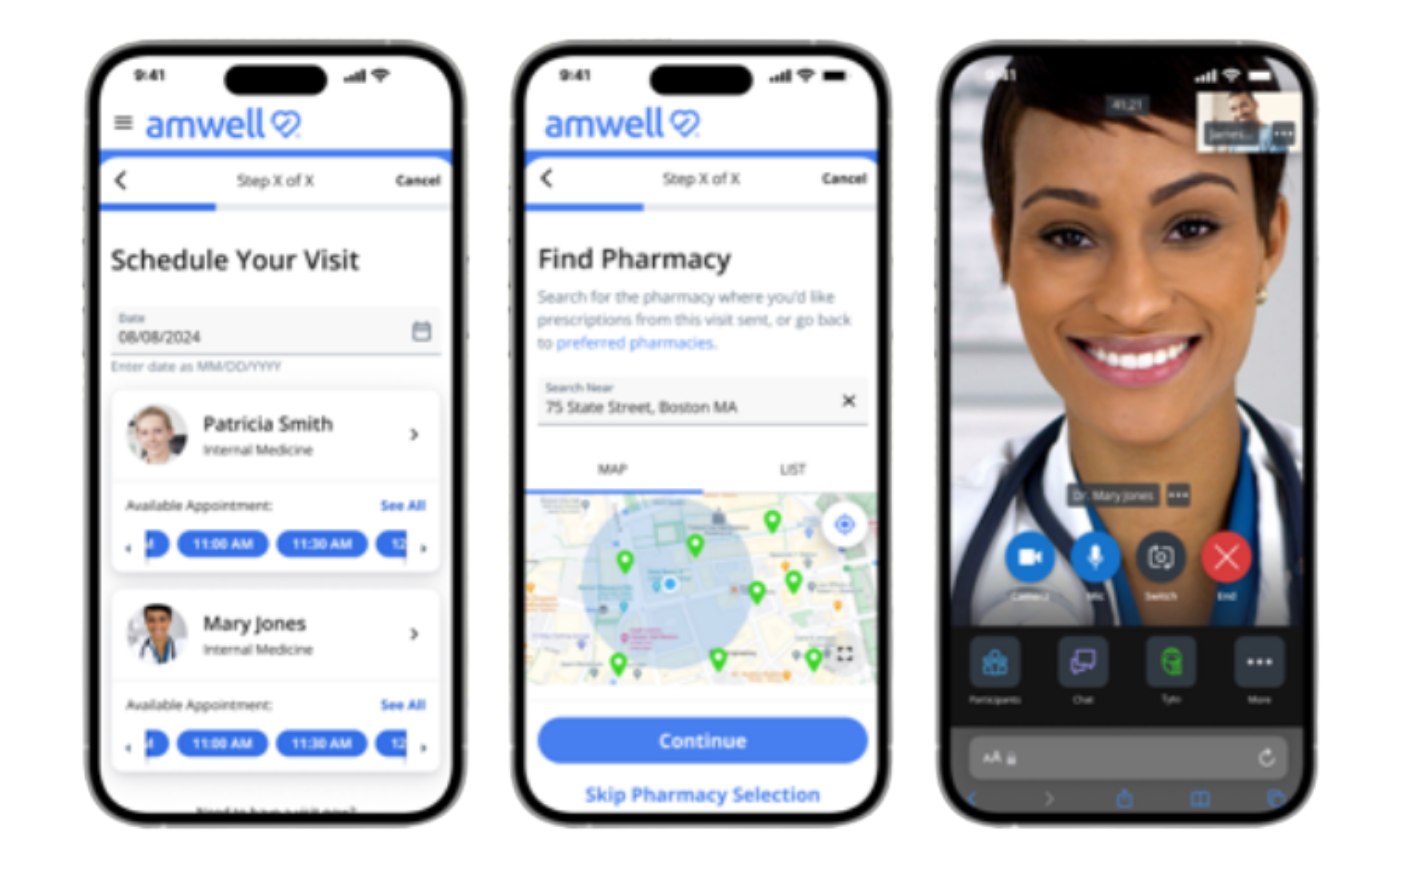
\includegraphics[width=0.9\textwidth]{amwell.png}
    \caption{Amwell Application Interface}
    \label{fig:amwell}
\end{figure}

\textbf{Strengths:} Online medical consultation, appointment management, access to medical records.\\
\textbf{Limitations:} Unattractive interface, absence of instant messaging, no AI assisted diagnosis, no recovery tracking.

\subsubsection{NHS App}

\textbf{NHS App} is the official application of the British National Health Service. It allows users to organize appointment bookings with doctors and consult their medical records.

\begin{figure}[H]
    \centering
    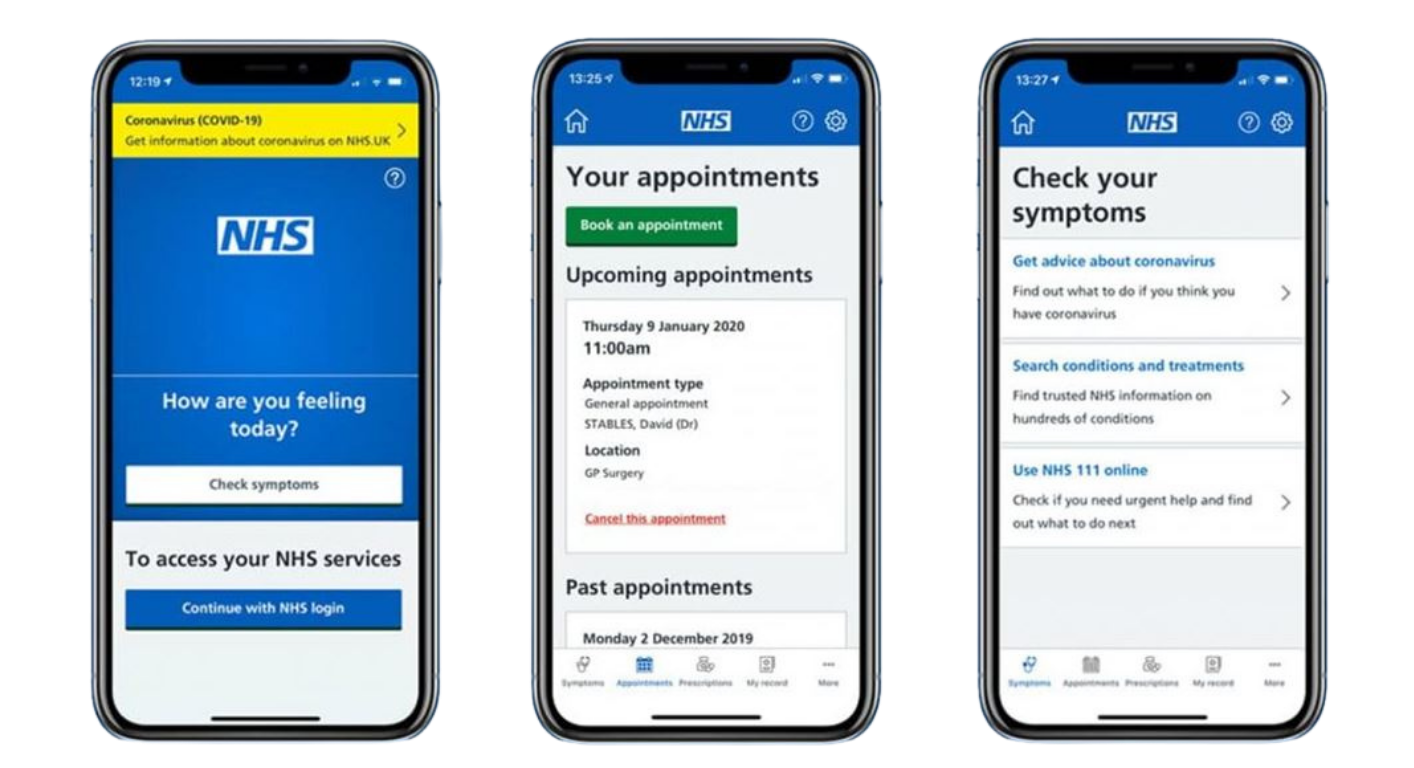
\includegraphics[width=0.9\textwidth]{nhs.png}
    \caption{NHS App Interface}
    \label{fig:nhs}
\end{figure}

\textbf{Strengths:} Access to medical records, appointment management.\\
\textbf{Limitations:} No video teleconsultation, no instant messaging, no clinical AI, too professionally oriented.

\subsubsection{Medisafe}

\textbf{Medisafe} is a personal health management application focused on medication tracking. It helps users track their medication intake through scheduled reminders.

\begin{figure}[H]
    \centering
    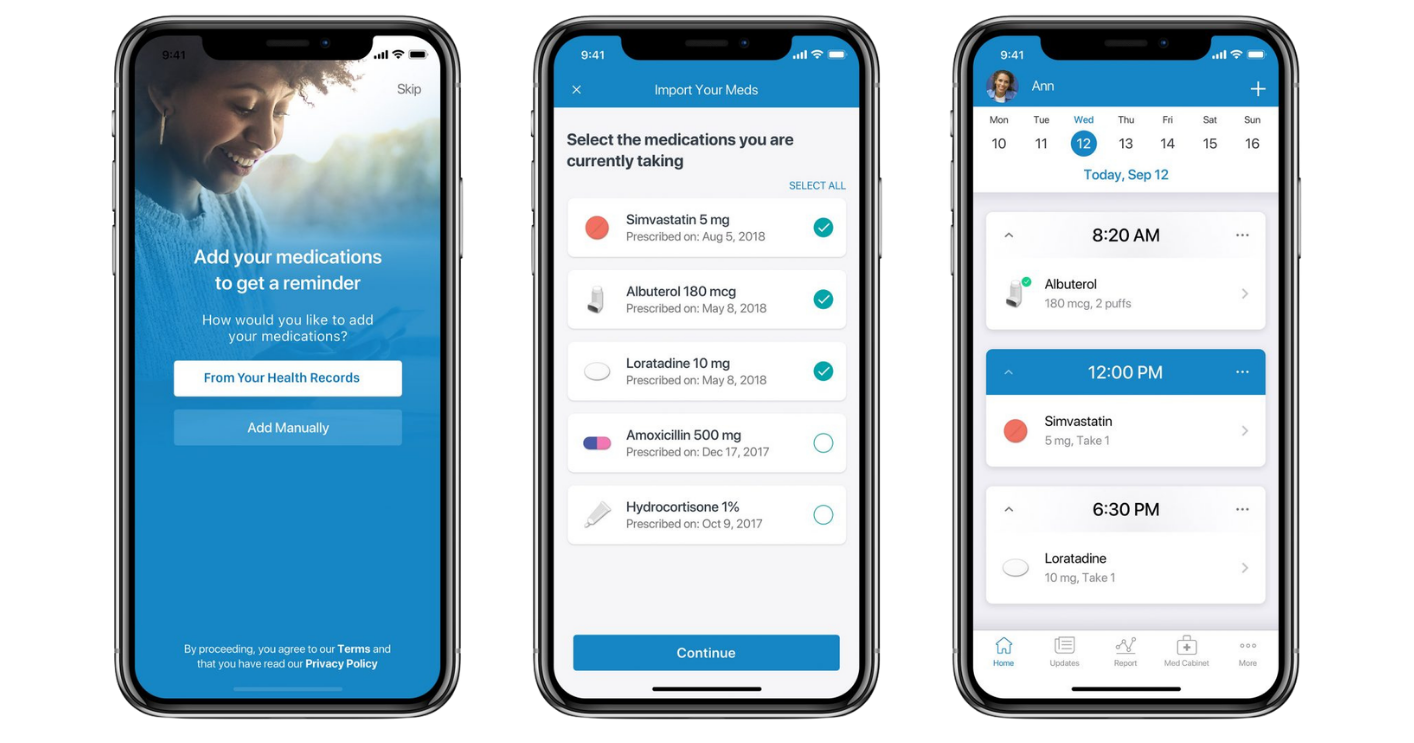
\includegraphics[width=0.9\textwidth]{medisafe.png}
    \caption{Medisafe Application Interface}
    \label{fig:medisafe}
\end{figure}

\textbf{Strengths:} Medication tracking, intake reminders.\\
\textbf{Limitations:} Features limited to medication management, no consultations, no complete medical record, no doctor patient communication.

\subsubsection{Doctolib}

\textbf{Doctolib} is the reference platform in France for online medical appointment booking. It connects patients with healthcare professionals.

\begin{figure}[H]
    \centering
    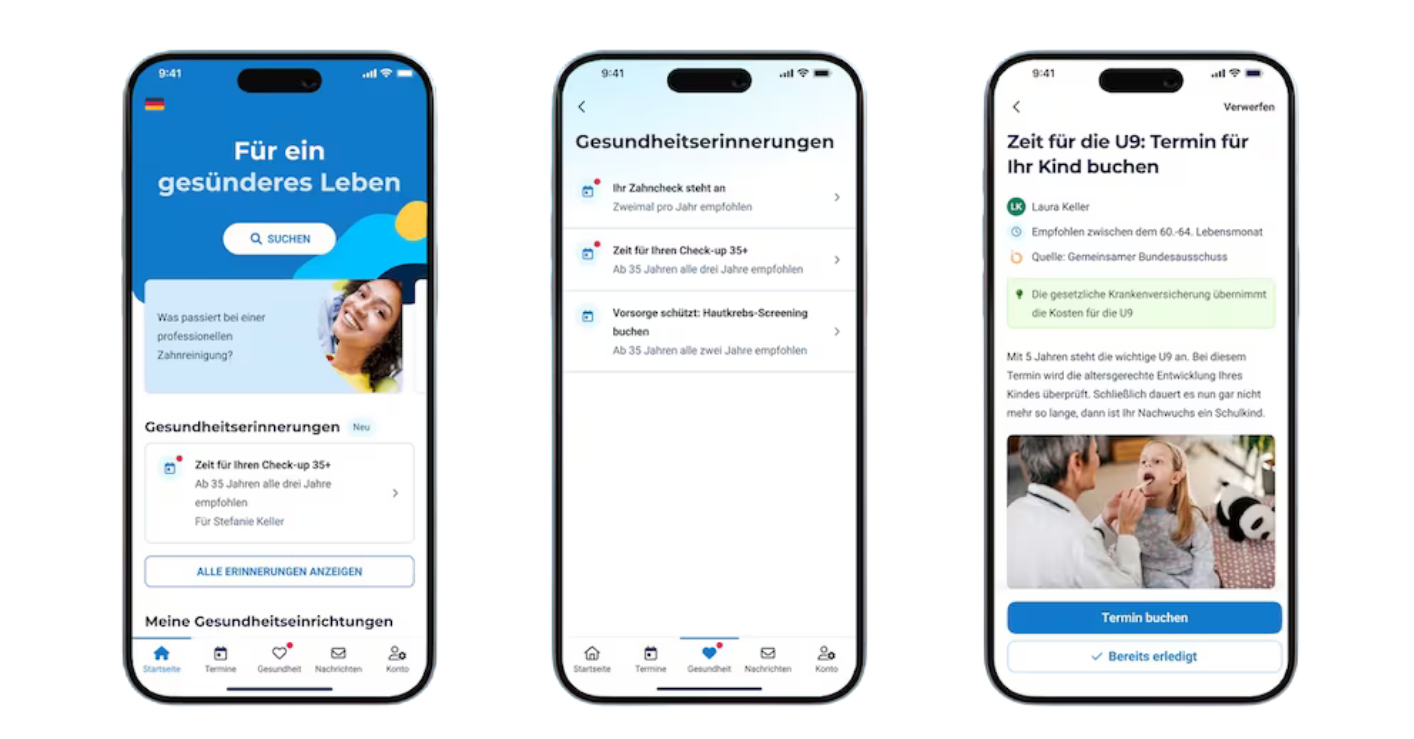
\includegraphics[width=0.9\textwidth]{doctolib.png}
    \caption{Doctolib Application Interface}
    \label{fig:doctolib}
\end{figure}

\textbf{Strengths:} Efficient online appointment booking, teleconsultation, large practitioner network.\\
\textbf{Limitations:} No integrated medical records, no recovery tracking, no clinical AI, no real time chat with doctors.

\subsection{Critique of Existing Solutions}

After analyzing existing solutions, we identified the following shortcomings:

\begin{itemize}
    \item \textbf{Amwell:} The interface is perceived as visually unattractive. Technical support is difficult to access. The application offers no artificial intelligence tools for diagnostic assistance.
    \item \textbf{NHS App:} The application lacks advanced features such as instant messaging and video teleconsultation. It is too oriented toward healthcare professionals.
    \item \textbf{Medisafe:} Features are limited to medication management. No integration with medical records, laboratory results, or consultations.
    \item \textbf{Doctolib:} Excellent for appointment booking but does not offer integrated medical records, recovery tracking, or clinical AI tools.
\end{itemize}

\textbf{Critique conclusion:} No existing application offers an integrated solution combining appointment management, complete medical records, medication tracking with adherence, laboratory results, AI assisted diagnosis, video telemedicine, real time messaging, and a composite recovery index. It is this gap that needs to be filled.

\subsection{Comparative Study}

We classify the results of our analysis according to the major functional criteria identified in our specifications. Table~\ref{tab:comparative} presents this comparison.

\begin{table}[H]
\centering
\caption{Comparative Table of Existing Healthcare Applications}
\label{tab:comparative}
\small
\begin{tabular}{|l|c|c|c|c|}
\hline
\textbf{Criterion} & \textbf{Amwell} & \textbf{NHS} & \textbf{Medisafe} & \textbf{Doctolib} \\
\hline
Video consultation        & Yes & No  & No  & Yes \\
\hline
Appointment management    & Yes & Yes & No  & Yes \\
\hline
Integrated medical record & Yes & Yes & No  & No \\
\hline
Instant messaging         & No  & No  & No  & No \\
\hline
Medication tracking       & No  & No  & Yes & No \\
\hline
AI symptom triage         & No  & No  & No  & No \\
\hline
AI diagnostic assistance  & No  & No  & No  & No \\
\hline
Laboratory results        & No  & Partial & No & No \\
\hline
Recovery index            & No  & No  & No  & No \\
\hline
Admin dashboard           & No  & No  & No  & Partial \\
\hline
Internationalization      & No  & No  & Yes & Partial \\
\hline
Zero Trust security       & No  & No  & No  & No \\
\hline
\end{tabular}
\end{table}

A visual representation of this comparison is provided in Figure~\ref{fig:comparative chart}.

\begin{figure}[H]
    \centering
    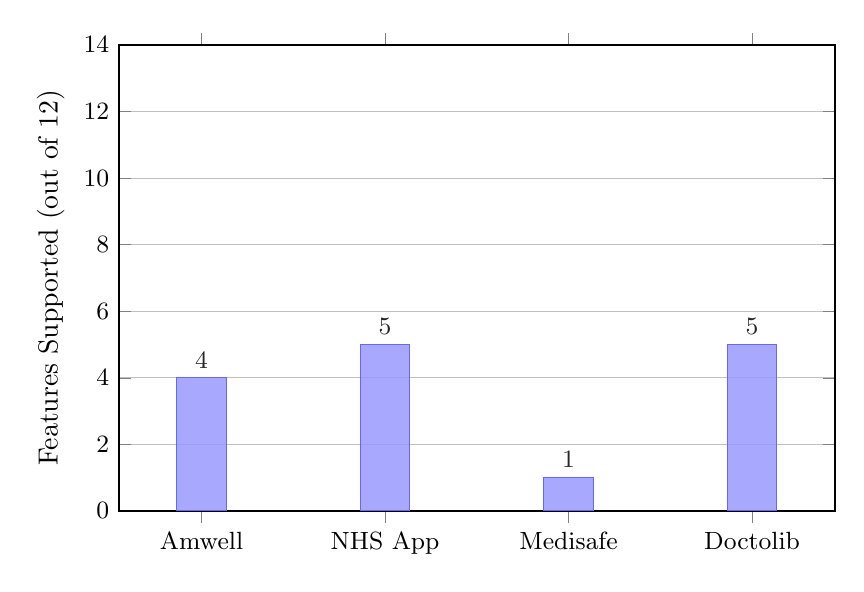
\begin{tikzpicture}
    \begin{axis}[
        ybar,
        bar width=18pt,
        width=0.88\textwidth,
        height=7.5cm,
        ylabel={Features Supported (out of 12)},
        ymin=0, ymax=14,
        ytick={0,2,4,6,8,10,12,14},
        symbolic x coords={Amwell, NHS App, Medisafe, Doctolib},
        xtick=data,
        x tick label style={font=\small},
        y tick label style={font=\small},
        nodes near coords,
        nodes near coords style={font=\small\bfseries},
        every axis plot/.append style={fill opacity=0.85},
        enlarge x limits=0.15,
        grid=major,
        ymajorgrids=true,
        xmajorgrids=false,
        axis line style={thick},
    ]
    \addplot[fill=blue!40, draw=blue!60] coordinates {
        (Amwell, 4) (NHS App, 5) (Medisafe, 1) (Doctolib, 5)
    };
    \end{axis}
    \end{tikzpicture}
    \caption{Feature Coverage Comparison of Healthcare Applications}
    \label{fig:comparative chart}
\end{figure}

\section{Proposed Solution}

After detailing our problem statement and analyzing the different existing solutions, the following question arises: can the applications available on the market represent a solution that addresses our problem?

Existing applications are either too general or limited to a single aspect of medical management (appointments, or medications, or teleconsultation), and often expensive. We need a specific, integrated solution that perfectly meets the needs specified by the client company.

The primary objective of this project is to design and develop \textbf{DocTIP}, a comprehensive medical platform dedicated to integrated medical practice management and intelligent patient recovery monitoring. The specific objectives are as follows:

\begin{itemize}
    \item \textbf{Centralize medical data} in a secure PostgreSQL relational database covering the entire medical lifecycle.
    \item \textbf{Develop a cross platform mobile application} (iOS and Android) covering patient, doctor, and shared portals.
    \item \textbf{Implement a web based administration dashboard} for global platform supervision.
    \item \textbf{Integrate artificial intelligence modules} for symptom triage, differential diagnosis assistance, clinical note generation, health risk prediction, and appointment optimization.
    \item \textbf{Establish a telemedicine system} with real time video and audio calls.
    \item \textbf{Design a Zero Trust security model} with login anomaly detection, device fingerprinting, and comprehensive audit logging.
    \item \textbf{Compute a weighted composite Patient Recovery Index (PRI)} integrating medication adherence, laboratory result trends, patient engagement, and physician evaluation.
    \item \textbf{Support internationalization} with three languages (French, English, Arabic) and three currencies (TND, EUR, USD).
\end{itemize}

We propose in this project to develop \textbf{DocTIP}, a comprehensive medical platform composed of three interconnected portals: a cross platform mobile application offering a patient portal, a doctor portal, shared features, and an authentication flow; a web based administration dashboard covering all platform data; and a serverless backend with a PostgreSQL database, Edge Functions, an authentication system with Row Level Security, and real time subscriptions.

The solution integrates the following functional modules:

\begin{itemize}
    \item \textbf{Medical Records Module:} Manages access, updates, and security of patient medical records.
    \item \textbf{Laboratory Analysis Module:} Facilitates requesting and consulting analysis results with biomarker trend tracking and anomaly detection.
    \item \textbf{Communication Module:} Enables patients and doctors to communicate via a real time messaging system supporting text, images, and files, as well as video/audio calls via Agora RTC.
    \item \textbf{Appointment Booking Module:} Allows patients to schedule appointments with AI optimization of time slots, support for three visit types (clinic, home, video), and an interactive calendar.
    \item \textbf{Artificial Intelligence Module:} Specialized AI functions including symptom triage, differential diagnosis, drug interaction verification, SOAP note generation, risk prediction, and behavioral analysis.
    \item \textbf{Recovery Monitoring Module:} Automatic computation of the Patient Recovery Index (PRI) a weighted composite score from 0 to 100.
    \item \textbf{Security Module:} Zero Trust architecture with login anomaly detection, device fingerprinting, audit logging, and Row Level Security.
    \item \textbf{Medication Management Module:} Dose by dose tracking (taken/missed/skipped), automatic reminders via cron every 15 minutes, computed adherence rate, medication delivery orders.
    \item \textbf{Mental Health Module:} Longitudinal tracking of mood, anxiety, sleep, and stress with trend visualization.
    \item \textbf{Emergency Module:} SOS mode with countdown, GPS geolocation, automatic emergency services call, treating physician notification.
\end{itemize}

\section{Requirements Analysis and Specification}

Taking into account the preliminary study conducted previously, it is necessary to determine the specifications of functional and non functional requirements, and to identify the different system actors.

\subsection{Actor Identification}

An actor is an entity external to the modeled system that interacts directly with it. Our project comprises three main actors, each with specific features and a dedicated portal:

\begin{itemize}
    \item \textbf{Patient:} Primary user of the mobile application. They browse the list of doctors, book appointments, access their medical record, track their medications, receive notifications, and communicate with their doctors.
    \item \textbf{Doctor:} Healthcare professional who manages their patients, establishes diagnoses, writes prescriptions, requests lab analyses, plans operations, and uses clinical AI tools.
    \item \textbf{DocTIP Administrator:} Responsible for platform supervision. They manage doctor access (approval/rejection), monitor patient activity, moderate complaints, consult platform analytics, and supervise AI modules.
\end{itemize}

\subsection{Functional Requirements}

In order to develop a coherent and complete system, a requirements specification phase is considered very important. It enables cataloging the system's features and defining its functional architecture. Functional requirements are organized by actor.

\subsubsection{Common Functional Requirements}

All actors can:

\begin{itemize}
    \item Authenticate: Every user can authenticate via Supabase Auth to access their workspace. The system supports registration with role selection (doctor/patient/admin).
    \item Manage their profile: Every user can view and modify their personal information (first name, last name, phone, date of birth, gender, address, profile picture).
    \item Receive notifications: The system sends push notifications for appointments, medications, lab results, messages, and security alerts.
    \item Configure the application: Language selection (French, English, Arabic), currency selection (TND, EUR, USD), and dark mode toggle.
\end{itemize}

\subsubsection{Patient Functional Requirements}

The patient can:

\begin{itemize}
    \item Browse the list of doctors: Search doctors by specialty, view on an interactive map, and filter by price and rating.
    \item Book an appointment: Select a doctor, choose a visit type (clinic, home, video), pick a date and time slot, benefit from intelligent sorting (condition $\rightarrow$ doctor specialty matching).
    \item Manage their appointments: View history, cancel with reason, reschedule, launch a video call.
    \item Create and update their medical record: Enter health information (blood type, height, weight, chronic diseases, allergies, surgical history, family history, lifestyle).
    \item View clinical records: Laboratory results with trend charts, prescriptions, diagnoses, surgical schedules.
    \item Track their medications: Daily dashboard with adherence progress ring, mark doses as taken/missed, and search medications in the directory.
    \item Use AI triage: Describe symptoms to receive an urgency assessment, possible conditions, recommended specialty, and follow up questions.
    \item Chat: Real time messaging with doctors (text, images, files), online presence indicators.
    \item Make video/audio calls: Teleconsultation with camera toggle, mute, speaker.
    \item Access advanced AI analytics: Longitudinal health intelligence, predictive risk scores (cardiovascular, diabetes, hospitalization), smart follow up plan, behavioral analysis (mood, stress, burnout), billing analysis.
    \item Use emergency mode: SOS with countdown, automatic call to emergency services, GPS geolocation, nearby hospitals map, emergency medical record sharing.
    \item Manage complaints: Submit and track complaints for encountered issues.
\end{itemize}

\subsubsection{Doctor Functional Requirements}

The doctor can:

\begin{itemize}
    \item Manage their patients: View the patient list, access detailed profiles with three tabs (Overview, Records, Notes).
    \item Manage prescriptions: Create multi medication prescriptions with dosage, frequency, administration route, duration, and time slots. View prescription history.
    \item View their appointments: Interactive monthly calendar with heat map, day view, status management.
    \item Establish a diagnosis: Examine symptoms, make a diagnosis with ICD code, indicate severity.
    \item Use AI differential diagnosis: Enter symptoms, examination results, history, and obtain diagnoses ranked by confidence with red flags, missing tests, and clinical pearls.
    \item Request lab analyses: Draft and send analysis requests with priority, view results with per biomarker trend charts.
    \item Plan operations: Organize surgical interventions with pre and post operative instructions.
    \item Write clinical notes: AI assisted generation of SOAP notes with auto suggestion of medical terms and ICD 10 codes.
    \item Use Voice Scribe: Voice dictation of clinical notes with 4 templates (progress note, procedure note, discharge summary), AI polish into professional clinical text.
    \item Interact with ORION: Persistent clinical AI chatbot with drug interaction checker, differential diagnosis, clinical guidelines, and dosage calculator.
    \item Monitor risk radar: Real time dashboard of all patients by risk score, adherence rate, deterioration detection.
    \item View per patient AI analytics: Health intelligence, predictive risks, follow up plan, behavioral analysis, emergency mode, billing analysis all individually per patient.
    \item Manage professional profile: 4 step setup wizard (personal, location with 10 countries and GPS, medical with 24 specialties, practice with rates and availability).
    \item Research mode: Anonymized analysis of aggregate data from all patients for epidemiological insights.
\end{itemize}

\subsubsection{Administrator Functional Requirements}

The DocTIP administrator can:

\begin{itemize}
    \item Supervise the dashboard: Real time KPIs (patients, doctors, appointments, prescriptions, lab results, average PRI), specialty distribution chart, monthly trend curves, recent activity feed.
    \item Manage doctors: Approve, reject, or suspend doctor accounts. View profile details, schedules, and schedule exceptions.
    \item Manage patients: View enriched profiles (blood type, allergies, conditions, PRI score), activity, and medical records.
    \item Manage appointments: Filter by status, visit type, and date. Modify statuses. View status change history.
    \item Manage prescriptions: Filter by status, view prescription items with per dose adherence tracking.
    \item Manage laboratory results: View results with reference ranges, anomaly flags, and trends. Manage analysis requests along the processing cycle.
    \item Moderate reviews: View and delete inappropriate reviews of doctors.
    \item Supervise messaging: Read only view of conversations and message threads.
    \item Manage notifications: Filter by type, send broadcast notifications (all/patients/doctors).
    \item Manage complaints: Status pipeline (open, in review, resolved, dismissed), resolution notes.
    \item View analytics: User growth, appointments by type and status, specialty rankings, triage by urgency, completion rates, average PRI score.
    \item Monitor AI: Triage sessions (risk score, urgency, recommended specialty), AI chat sessions, urgency distribution.
    \item Manage diagnoses, operations, consultation reports, video sessions, medication orders, clinical notes, mental health logs, and attachments.
    \item Configure the platform: Name, timezone, language, maintenance mode, max daily appointments, auto approval, 2FA, session duration, notification channels.
\end{itemize}

\subsection{Non Functional Requirements}

Non functional requirements represent internal application requirements essential for guaranteeing an optimal user experience and system security:

\begingroup
\renewcommand{\labelitemii}{\textbullet}
\begin{itemize}
    \item \textbf{Security:}
    \begin{itemize}
        \item Authentication via Supabase Auth with secure JWT tokens and automatic refresh.
        \item Row Level Security (RLS): row level security policies for every table, ensuring each user can only access their own data.
        \item Zero Trust architecture: login anomaly detection (new device, unusual location, abnormal time, multiple failed attempts, impossible travel), risk scoring (0 to 100), automatic alert for scores $\geq 30$, 2FA requirement for scores $\geq 50$.
        \item Device fingerprinting and comprehensive audit logging.
    \end{itemize}
    \item \textbf{Performance:}
    \begin{itemize}
        \item Serverless architecture for automatic scaling.
        \item Optimized database indexes on all frequently queried columns.
        \item Real time subscriptions for messaging, notifications, and online presence.
        \item Offline cache (AsyncStorage) for medication data and AI sessions.
    \end{itemize}
    \item \textbf{Maintainability:}
    \begin{itemize}
        \item Strict TypeScript across the entire project (mobile, web, edge functions).
        \item Modular architecture: separation into layers (screens, components, stores, services, navigation).
        \item Reusable UI components (Button, Card, Avatar, Badge, ProgressRing, etc.).
        \item 7 Zustand stores for state management.
    \end{itemize}
    \item \textbf{Usability:}
    \begin{itemize}
        \item Premium user interface with fluid animations (Framer Motion for web, React Native Animated for mobile).
        \item Haptic feedback on mobile (expo haptics) for touch interactions.
        \item Right to left (RTL) writing support for Arabic.
        \item Rich visual components: progress rings, trend charts, interactive maps.
    \end{itemize}
    \item \textbf{Availability:}
    \begin{itemize}
        \item Managed Supabase infrastructure with high availability.
        \item Partial offline mode for medication management.
        \item Cross platform support: iOS, Android, and Web.
    \end{itemize}
    \item \textbf{Internationalization:}
    \begin{itemize}
        \item 3 languages: French, English, Arabic (with over 100 translation keys).
        \item 3 currencies: TND, EUR, USD with adapted formatting.
    \end{itemize}
\end{itemize}
\endgroup

\section{Work Methodology}

Effective project management involves the use of an appropriate methodology to ensure the smooth progression of work through to completion, taking into account client needs and potential changes.

\subsection{Agile Methodology}

For the development of this project, we adopted the \textbf{Agile Scrum methodology}~\cite{agile}. Given the complexity and technological diversity of the platform, we needed a rigorous yet adaptable approach. The project combines information system design and modeling with mobile, web, and backend development, which requires continuous alignment between analysis and implementation. A structured methodology ensures traceability of requirements, consistent quality across phases, and controlled risk management, while preserving the flexibility to integrate feedback and accommodate changes in scope. In this context, selecting an appropriate development approach is essential. We therefore chose Scrum, an agile framework that emphasizes collaboration, transparency, and continuous improvement. Scrum structures work around a prioritized product backlog, a sprint backlog selected for a short time boxed iteration, and a potentially usable increment produced at the end of each sprint. Short cycles allow early validation, rapid feedback, and tighter control of timelines and costs. Daily scrum meetings keep communication fluid and enable quick decision making, while sprint reviews and retrospectives ensure alignment and continuous improvement. This choice is motivated by several considerations specific to the project context:

\begin{itemize}
    \item \textbf{Rapid iterations:} The project comprises multiple interfaces to develop. Scrum allows dividing this volume into 2 week sprints, each delivering a testable functional increment.
    \item \textbf{Adaptability:} The AI and telemedicine modules require frequent adjustments based on test feedback. Agility enables rapid integration of this feedback.
    \item \textbf{Value based prioritization:} Features are prioritized by business value (authentication and medical records first, clinical AI next, advanced features last).
    \item \textbf{Continuous delivery:} Each sprint produces a deployable increment, enabling regular validation with the client.
\end{itemize}

\vspace{0.6cm}
\begin{figure}[H]
    \centering
    
\includegraphics[width=\textwidth,keepaspectratio]{"figures/Scrum Project Management Process Infographic Presentation (1).png"}
    \caption{Professional Scrum Methodology Cycle for the DocTIP Project}
    \label{fig:scrum}
\end{figure}

\subsection{Product Backlog}

The Product Backlog is a prioritized list of features, functionalities, and requirements needed to build DocTIP. It is managed and continuously refined to reflect the most valuable requirements. Key epics include user authentication, AI symptom triage, appointment scheduling, video teleconsultation, and the clinical dashboard.

\begin{longtable}{|c|p{7.5cm}|c|c|}
\caption{DocTIP Platform Product Backlog}
\label{tab:product-backlog} \\
\hline
\textbf{ID} & \textbf{User Story / Feature} & \textbf{Priority} & \textbf{Sprint} \\
\hline
\endfirsthead
\hline
\textbf{ID} & \textbf{User Story / Feature} & \textbf{Priority} & \textbf{Sprint} \\
\hline
\endhead
\hline
\endfoot
\multicolumn{4}{|c|}{\textbf{Sprint 0: Analysis \& Planning}} \\
\hline
UI01 & As a project manager, I want to define the project scope and requirements so that the team has a clear vision. & High & 0 \\
\hline
UI02 & As a developer, I want to design the system architecture so that the technical foundation is well planned. & High & 0 \\
\hline
UI03 & As a developer, I want to create initial UML diagrams so that the system structure is documented. & High & 0 \\
\hline
UI04 & As a project manager, I want to establish the product backlog so that features are prioritized. & Medium & 0 \\
\hline
\multicolumn{4}{|c|}{\textbf{Sprint 1: Core Foundation}} \\
\hline
UI05 & As a developer, I want to set up the PostgreSQL database schema so that data can be stored securely. & High & 1 \\
\hline
UI06 & As a user, I want to register and authenticate so that I can access the platform securely. & High & 1 \\
\hline
UI07 & As a developer, I want to implement Row Level Security so that users can only access their own data. & High & 1 \\
\hline
UI08 & As a developer, I want to scaffold the project structure so that development can begin efficiently. & High & 1 \\
\hline
\multicolumn{4}{|c|}{\textbf{Sprint 2: Mobile Foundations}} \\
\hline
UI09 & As a patient, I want to complete an onboarding wizard so that my medical profile is initialized. & High & 2 \\
\hline
UI10 & As a user, I want to manage my profile so that my information is up to date. & High & 2 \\
\hline
UI11 & As a patient, I want to view my medical record so that I can track my health history. & High & 2 \\
\hline
UI12 & As a developer, I want to implement mobile navigation so that users can move between screens. & High & 2 \\
\hline
\multicolumn{4}{|c|}{\textbf{Sprint 3: Scheduling \& Medications}} \\
\hline
UI13 & As a patient, I want to book an appointment so that I can consult with a doctor. & High & 3 \\
\hline
UI14 & As a patient, I want to view my appointment calendar so that I can manage my schedule. & High & 3 \\
\hline
UI15 & As a doctor, I want to manage my schedule so that patients can book available slots. & High & 3 \\
\hline
UI16 & As a patient, I want to track my medications so that I can manage my treatment plan. & High & 3 \\
\hline
UI17 & As a patient, I want to receive medication reminders so that I never miss a dose. & Medium & 3 \\
\hline
\multicolumn{4}{|c|}{\textbf{Sprint 4: Labs \& Messaging}} \\
\hline
UI18 & As a patient, I want to view my lab results so that I can monitor my health status. & High & 4 \\
\hline
UI19 & As a patient, I want to upload lab reports with OCR so that results are digitized automatically. & Medium & 4 \\
\hline
UI20 & As a patient, I want to chat with my doctor so that I can communicate in real time. & High & 4 \\
\hline
UI21 & As a user, I want to share files in chat so that I can send medical documents. & Medium & 4 \\
\hline
\multicolumn{4}{|c|}{\textbf{Sprint 5: Clinical AI}} \\
\hline
UI22 & As a patient, I want to use AI symptom triage so that I can assess my urgency level. & High & 5 \\
\hline
UI23 & As a doctor, I want AI generated SOAP notes so that clinical documentation is faster. & High & 5 \\
\hline
UI24 & As a doctor, I want to interact with ORION AI assistant so that I can get clinical decision support. & Medium & 5 \\
\hline
UI25 & As a user, I want to make video calls so that I can have teleconsultations. & High & 5 \\
\hline
\multicolumn{4}{|c|}{\textbf{Sprint 6: Admin \& Analytics}} \\
\hline
UI26 & As an administrator, I want to manage doctor accounts so that I can approve or reject registrations. & High & 6 \\
\hline
UI27 & As an administrator, I want to view platform analytics so that I can monitor system performance. & High & 6 \\
\hline
UI28 & As an administrator, I want to manage complaints so that I can resolve user issues. & Medium & 6 \\
\hline
UI29 & As an administrator, I want to monitor AI usage so that I can track system health. & Medium & 6 \\
\hline
\multicolumn{4}{|c|}{\textbf{Sprint 7: Advanced Features}} \\
\hline
UI30 & As a patient, I want to view my Recovery Index so that I can track my recovery progress. & High & 7 \\
\hline
UI31 & As a patient, I want to use emergency mode so that I can get help in critical situations. & High & 7 \\
\hline
UI32 & As a patient, I want to see predictive risk scores so that I can prevent health issues. & Medium & 7 \\
\hline
UI33 & As a developer, I want to implement testing and optimization so that the platform is production ready. & High & 7 \\
\hline
\end{longtable}

\section{Planning}

Proper planning ensures that the project is executed systematically. It breaks down the development process into manageable sprints and establishes a clear timeline.

% ============================================================================
%                       SPRINT ORGANIZATION TABLE
% ============================================================================
\subsection{Sprint Planning}

Development was structured across well defined logical sprints to ensure continuous integration of features according to priority. Table~\ref{tab:sprints} summarizes the core deliverable per iteration.

\begin{table}[H]
    \centering
    \renewcommand{\arraystretch}{1.4}
    \caption{Sprint Planning for the DocTIP Project}
    \label{tab:sprints}
    \small
\begin{tabular}{|c|l|p{9cm}|}
\hline
        \textbf{Sprint} & \textbf{Module} & \textbf{Deliverables} \\
\hline
        0 & Analysis            & Requirements, project scope, architecture outline, UML diagrams \\
\hline
        1 & Core Foundation     & PostgreSQL schema, Supabase Auth, RLS, project scaffolding \\
\hline
        2 & Mobile Foundations  & Onboarding, user profiles, medical records, navigation \\
\hline
        3 & Scheduling \& Meds  & Appointments, calendar, prescriptions, medication tracking \\
\hline
        4 & Labs \& Messaging   & Lab results, trend visualization, real time chat, file sharing \\
\hline
        5 & Clinical AI         & AI triage, SOAP notes, ORION integration, video/audio calls \\
\hline
        6 & Admin \& Analytics  & Web dashboard, complaints management, AI monitoring, analytics \\
\hline
        7 & Advanced Features   & PRI integration, emergency handling, prediction models, deployment \\
\hline
    \end{tabular}
\end{table}

\clearpage
\subsection{Gantt Chart}

The project planning is represented by the Gantt chart below, which visualizes the temporal sequencing of the main tasks. Figure~\ref{fig:gantt} shows this planning.

\begin{figure}[H]
    \centering
    \resizebox{\textwidth}{!}{% DocTIP Gantt Chart (8 equal sprints × 2 units, Feb to May)
% Compiled inline by pdflatex via % DocTIP Gantt Chart (8 equal sprints × 2 units, Feb to May)
% Compiled inline by pdflatex via % DocTIP Gantt Chart (8 equal sprints × 2 units, Feb to May)
% Compiled inline by pdflatex via \input{figures/tikz/gantt-chart.tex}
\begin{ganttchart}[
    hgrid,
    vgrid,
    x unit=0.56cm,
    y unit title=0.72cm,
    y unit chart=0.58cm,
    title label font=\scriptsize\bfseries,
    bar label font=\scriptsize,
    bar/.append style={fill=orange!80, draw=orange!80},
    bar height=0.48,
    title height=1,
]{1}{16}
  \gantttitle{2026 Project Timeline}{16} \\
  \gantttitle{Feb}{4}\gantttitle{Mar}{4}\gantttitle{Apr}{4}\gantttitle{May}{4} \\

  \ganttbar{Sprint 0: Analysis}{1}{2} \\
  \ganttbar{Sprint 1: Core Foundation}{3}{4} \\
  \ganttbar{Sprint 2: Mobile Foundations}{5}{6} \\
  \ganttbar{Sprint 3: Scheduling and Meds}{7}{8} \\
  \ganttbar{Sprint 4: Labs and Messaging}{9}{10} \\
  \ganttbar{Sprint 5: Clinical AI and Telemedicine}{11}{12} \\
  \ganttbar{Sprint 6: Admin and Analytics}{13}{14} \\
  \ganttbar{Sprint 7: Advanced Features}{15}{16} \\
  \ganttbar{Report writing and documentation}{1}{16}
\end{ganttchart}


\begin{ganttchart}[
    hgrid,
    vgrid,
    x unit=0.56cm,
    y unit title=0.72cm,
    y unit chart=0.58cm,
    title label font=\scriptsize\bfseries,
    bar label font=\scriptsize,
    bar/.append style={fill=orange!80, draw=orange!80},
    bar height=0.48,
    title height=1,
]{1}{16}
  \gantttitle{2026 Project Timeline}{16} \\
  \gantttitle{Feb}{4}\gantttitle{Mar}{4}\gantttitle{Apr}{4}\gantttitle{May}{4} \\

  \ganttbar{Sprint 0: Analysis}{1}{2} \\
  \ganttbar{Sprint 1: Core Foundation}{3}{4} \\
  \ganttbar{Sprint 2: Mobile Foundations}{5}{6} \\
  \ganttbar{Sprint 3: Scheduling and Meds}{7}{8} \\
  \ganttbar{Sprint 4: Labs and Messaging}{9}{10} \\
  \ganttbar{Sprint 5: Clinical AI and Telemedicine}{11}{12} \\
  \ganttbar{Sprint 6: Admin and Analytics}{13}{14} \\
  \ganttbar{Sprint 7: Advanced Features}{15}{16} \\
  \ganttbar{Report writing and documentation}{1}{16}
\end{ganttchart}


\begin{ganttchart}[
    hgrid,
    vgrid,
    x unit=0.56cm,
    y unit title=0.72cm,
    y unit chart=0.58cm,
    title label font=\scriptsize\bfseries,
    bar label font=\scriptsize,
    bar/.append style={fill=orange!80, draw=orange!80},
    bar height=0.48,
    title height=1,
]{1}{16}
  \gantttitle{2026 Project Timeline}{16} \\
  \gantttitle{Feb}{4}\gantttitle{Mar}{4}\gantttitle{Apr}{4}\gantttitle{May}{4} \\

  \ganttbar{Sprint 0: Analysis}{1}{2} \\
  \ganttbar{Sprint 1: Core Foundation}{3}{4} \\
  \ganttbar{Sprint 2: Mobile Foundations}{5}{6} \\
  \ganttbar{Sprint 3: Scheduling and Meds}{7}{8} \\
  \ganttbar{Sprint 4: Labs and Messaging}{9}{10} \\
  \ganttbar{Sprint 5: Clinical AI and Telemedicine}{11}{12} \\
  \ganttbar{Sprint 6: Admin and Analytics}{13}{14} \\
  \ganttbar{Sprint 7: Advanced Features}{15}{16} \\
  \ganttbar{Report writing and documentation}{1}{16}
\end{ganttchart}

}
    \caption{DocTIP Project Gantt Chart}
    \label{fig:gantt}
\end{figure}

% The TikZ/pgfgantt source for this figure is in: figures/gantt chart.tex
% Compile it standalone or include it inline using % DocTIP Gantt Chart (8 equal sprints × 2 units, Feb to May)
% Compiled inline by pdflatex via % DocTIP Gantt Chart (8 equal sprints × 2 units, Feb to May)
% Compiled inline by pdflatex via % DocTIP Gantt Chart (8 equal sprints × 2 units, Feb to May)
% Compiled inline by pdflatex via \input{figures/tikz/gantt-chart.tex}
\begin{ganttchart}[
    hgrid,
    vgrid,
    x unit=0.56cm,
    y unit title=0.72cm,
    y unit chart=0.58cm,
    title label font=\scriptsize\bfseries,
    bar label font=\scriptsize,
    bar/.append style={fill=orange!80, draw=orange!80},
    bar height=0.48,
    title height=1,
]{1}{16}
  \gantttitle{2026 Project Timeline}{16} \\
  \gantttitle{Feb}{4}\gantttitle{Mar}{4}\gantttitle{Apr}{4}\gantttitle{May}{4} \\

  \ganttbar{Sprint 0: Analysis}{1}{2} \\
  \ganttbar{Sprint 1: Core Foundation}{3}{4} \\
  \ganttbar{Sprint 2: Mobile Foundations}{5}{6} \\
  \ganttbar{Sprint 3: Scheduling and Meds}{7}{8} \\
  \ganttbar{Sprint 4: Labs and Messaging}{9}{10} \\
  \ganttbar{Sprint 5: Clinical AI and Telemedicine}{11}{12} \\
  \ganttbar{Sprint 6: Admin and Analytics}{13}{14} \\
  \ganttbar{Sprint 7: Advanced Features}{15}{16} \\
  \ganttbar{Report writing and documentation}{1}{16}
\end{ganttchart}


\begin{ganttchart}[
    hgrid,
    vgrid,
    x unit=0.56cm,
    y unit title=0.72cm,
    y unit chart=0.58cm,
    title label font=\scriptsize\bfseries,
    bar label font=\scriptsize,
    bar/.append style={fill=orange!80, draw=orange!80},
    bar height=0.48,
    title height=1,
]{1}{16}
  \gantttitle{2026 Project Timeline}{16} \\
  \gantttitle{Feb}{4}\gantttitle{Mar}{4}\gantttitle{Apr}{4}\gantttitle{May}{4} \\

  \ganttbar{Sprint 0: Analysis}{1}{2} \\
  \ganttbar{Sprint 1: Core Foundation}{3}{4} \\
  \ganttbar{Sprint 2: Mobile Foundations}{5}{6} \\
  \ganttbar{Sprint 3: Scheduling and Meds}{7}{8} \\
  \ganttbar{Sprint 4: Labs and Messaging}{9}{10} \\
  \ganttbar{Sprint 5: Clinical AI and Telemedicine}{11}{12} \\
  \ganttbar{Sprint 6: Admin and Analytics}{13}{14} \\
  \ganttbar{Sprint 7: Advanced Features}{15}{16} \\
  \ganttbar{Report writing and documentation}{1}{16}
\end{ganttchart}


\begin{ganttchart}[
    hgrid,
    vgrid,
    x unit=0.56cm,
    y unit title=0.72cm,
    y unit chart=0.58cm,
    title label font=\scriptsize\bfseries,
    bar label font=\scriptsize,
    bar/.append style={fill=orange!80, draw=orange!80},
    bar height=0.48,
    title height=1,
]{1}{16}
  \gantttitle{2026 Project Timeline}{16} \\
  \gantttitle{Feb}{4}\gantttitle{Mar}{4}\gantttitle{Apr}{4}\gantttitle{May}{4} \\

  \ganttbar{Sprint 0: Analysis}{1}{2} \\
  \ganttbar{Sprint 1: Core Foundation}{3}{4} \\
  \ganttbar{Sprint 2: Mobile Foundations}{5}{6} \\
  \ganttbar{Sprint 3: Scheduling and Meds}{7}{8} \\
  \ganttbar{Sprint 4: Labs and Messaging}{9}{10} \\
  \ganttbar{Sprint 5: Clinical AI and Telemedicine}{11}{12} \\
  \ganttbar{Sprint 6: Admin and Analytics}{13}{14} \\
  \ganttbar{Sprint 7: Advanced Features}{15}{16} \\
  \ganttbar{Report writing and documentation}{1}{16}
\end{ganttchart}



\section*{Conclusion}
\phantomsection
\addcontentsline{toc}{section}{Conclusion}

This chapter established the foundations of the DocTIP project. We presented the host organization, defined the project scope by identifying the gaps in existing solutions that motivated this initiative, and exhaustively specified the functional and non functional requirements of the three system actors. The comparative analysis demonstrated that no existing solution combines the totality of features targeted by DocTIP in particular the integration of clinical artificial intelligence, intelligent recovery monitoring, and Zero Trust security.

The following chapter will focus on the design phase, which will be explored in detail through UML diagrams and the architecture of the AI modules.


% ============================================================================
%                        CHAPTER 2 CONCEPTUAL DESIGN
% ============================================================================
\chapterflyleaf{Conceptual Design}
\chapter{Conceptual Design}

\section*{Introduction}
\phantomsection
\addcontentsline{toc}{section}{Introduction}

In the previous chapter, the different actors of the solution were identified by explicating the multiple available features. The current phase concerns design, a crucial step in application development. Throughout this chapter, we will present the use case diagrams (general and refined), the class diagram, the sequence diagrams, the activity diagrams, and the architecture of the artificial intelligence modules.

\section{UML Definition}

UML (\textit{Unified Modeling Language}) is an object oriented modeling language standardized by the Object Management Group in 1997. It results from the unification of methods proposed by Grady Booch, Ivar Jacobson, and Jim Rumbaugh, with the goal of providing a common and rigorous notation for software design~\cite{uml}. UML is widely adopted in software engineering because it improves understanding and communication, provides standardized notation, and supports multiple viewpoints of a system.

UML defines thirteen diagram types that cover structural and behavioral aspects. In this report, we focus on diagrams that best represent our solution from complementary perspectives: use case diagrams to describe the functional axis, a class diagram to describe the static structure, sequence diagrams to illustrate dynamic scenarios and interactions, and activity diagrams to model workflows and decision logic.

\begin{center}
    
\includegraphics[width=0.25\textwidth]{uml.png}
\end{center}

\clearpage
We model our system by creating the following UML diagrams:

\begin{itemize}
    \item Use case diagrams (general and refined)
    \item Class diagram
    \item Sequence diagrams
    \item Activity diagrams
\end{itemize}

\section{Use Case Diagrams}

The use case diagram describes the functional requirements of the system. Each use case corresponds to a business function of the system, from the viewpoint of one of its actors.

\subsection{General Use Case Diagram}

Figure~\ref{fig:use case general} represents the general use case diagram of our application, describing the global features accessible to each actor.

\begin{figure}[H]
    \centering
    \resizebox{\textwidth}{!}{% General Use Case Diagram
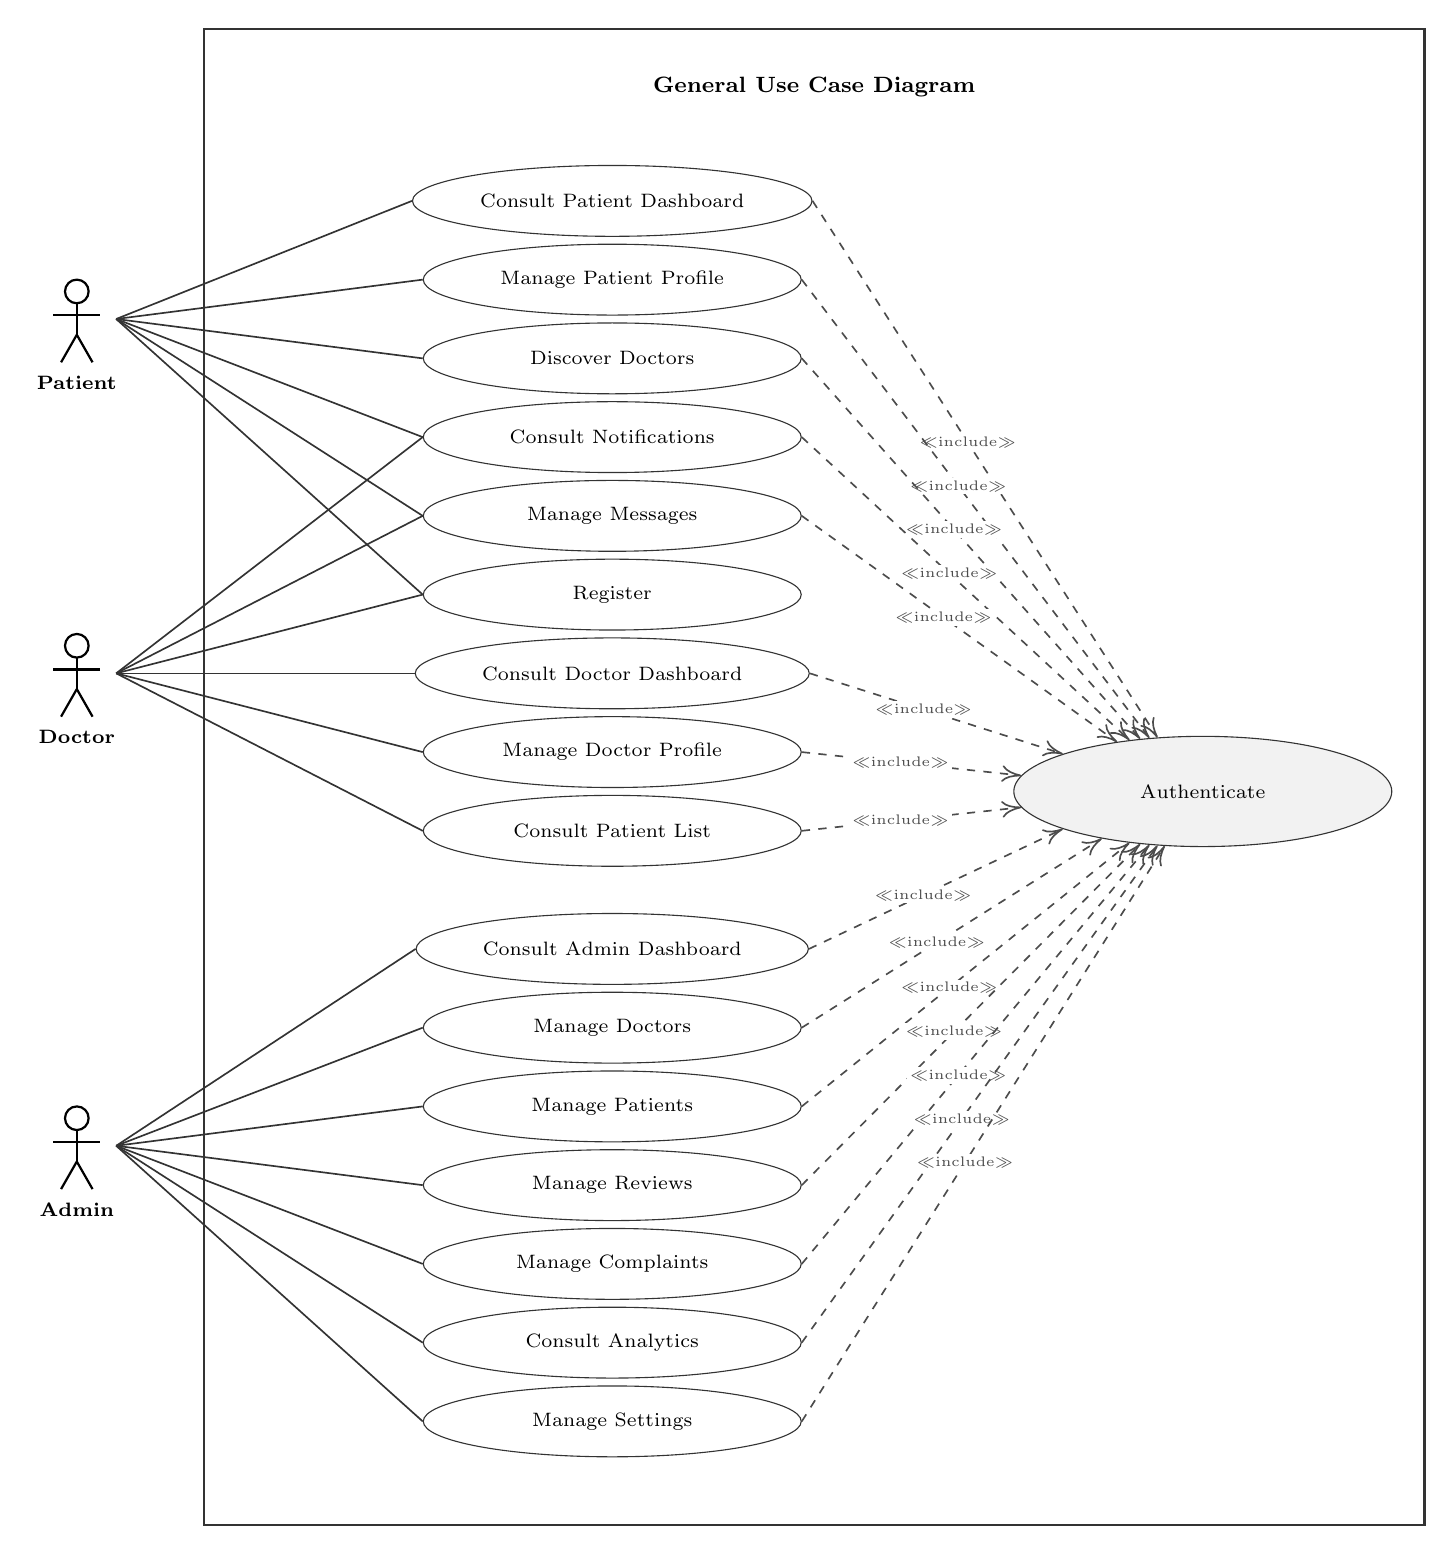
\begin{tikzpicture}[x=1cm,y=1cm]

% --- STYLES ---
\tikzset{
  actorlabel/.style={font=\scriptsize\bfseries, align=center},
  usecase/.style={ellipse, draw=black!80, fill=white,
                  font=\scriptsize, align=center,
                  minimum width=4.8cm, minimum height=0.9cm},
  boundary/.style={draw=black!80, line width=0.8pt},
  assoc/.style={black!80, line width=0.6pt},
  % Open vee arrowhead (>) as requested
  include/.style={black!70, dashed, line width=0.6pt,
                  -{>[length=7pt, width=6pt]}},
}

% --- ACTOR DRAWING MACRO ---
\newcommand{\actor}[3]{
  \begin{scope}[shift={(#1,#2)}]
    \draw[thick] (0,0.35) circle (0.15);
    \draw[thick] (0,0.20) -- (0,-0.2);
    \draw[thick] (-0.3,0.05) -- (0.3,0.05);
    \draw[thick] (0,-0.2) -- (-0.2,-0.55);
    \draw[thick] (0,-0.2) -- (0.2,-0.55);
    \node[actorlabel, below] at (0,-0.60) {#3};
  \end{scope}
}

% ================= SYSTEM BOUNDARY & TITLE =================
\node[boundary, minimum width=15.5cm, minimum height=19cm, anchor=north west]
      (sys) at (-0.2, 9.2) {};

\node[font=\footnotesize\bfseries, anchor=north]
      at ($(sys.north)+(0,-0.5)$) {General Use Case Diagram};

% ================= ACTORS =================
\actor{-1.8}{ 5.5}{Patient}
\actor{-1.8}{ 1.0}{Doctor}
\actor{-1.8}{-5.0}{Admin}

% ================= SHARED USE CASES (Patient & Doctor) =================
\node[usecase] (notif) at (5, 4.0) {Consult Notifications};
\node[usecase] (msg)   at (5, 3.0) {Manage Messages};
\node[usecase] (reg)   at (5, 2.0) {Register};

% ================= PATIENT-ONLY USE CASES =================
\node[usecase] (pdash) at (5, 7.0) {Consult Patient Dashboard};
\node[usecase] (pprof) at (5, 6.0) {Manage Patient Profile};
\node[usecase] (disc)  at (5, 5.0) {Discover Doctors};

% ================= DOCTOR-ONLY USE CASES =================
\node[usecase] (ddash) at (5, 1.0) {Consult Doctor Dashboard};
\node[usecase] (dprof) at (5, 0.0) {Manage Doctor Profile};
\node[usecase] (plist) at (5,-1.0) {Consult Patient List};

% ================= ADMIN USE CASES =================
\node[usecase] (adash) at (5,-2.5) {Consult Admin Dashboard};
\node[usecase] (mdoc)  at (5,-3.5) {Manage Doctors};
\node[usecase] (mpat)  at (5,-4.5) {Manage Patients};
\node[usecase] (mrev)  at (5,-5.5) {Manage Reviews};
\node[usecase] (mcomp) at (5,-6.5) {Manage Complaints};
\node[usecase] (anal)  at (5,-7.5) {Consult Analytics};
\node[usecase] (set)   at (5,-8.5) {Manage Settings};

% ================= AUTHENTICATION USE CASE =================
\node[usecase, minimum width=4.8cm, minimum height=1.4cm, fill=black!5]
      (auth) at (12.5, -0.5) {Authenticate};

% ================= ACTOR ASSOCIATIONS (Solid Lines) =================
\foreach \u in {pdash, pprof, disc, notif, msg, reg} {
    \draw[assoc] (-1.3, 5.5) -- (\u.west);
}

\foreach \u in {notif, msg, reg, ddash, dprof, plist} {
    \draw[assoc] (-1.3, 1.0) -- (\u.west);
}

\foreach \u in {adash, mdoc, mpat, mrev, mcomp, anal, set} {
    \draw[assoc] (-1.3, -5.0) -- (\u.west);
}

% ================= INCLUDE RELATIONSHIPS (Dashed Lines) =================
\foreach \u/\ang in {
    pdash/130, pprof/135, disc/140,
    notif/145, msg/150,
    ddash/165, dprof/175, plist/185,
    adash/195, mdoc/205, mpat/215,
    mrev/220, mcomp/225, anal/230, set/235
} {
    \draw[include] (\u.east) --
    node[pos=0.45, fill=white, inner sep=1pt, font=\tiny] {$\ll$include$\gg$}
    (auth.\ang);
}

\end{tikzpicture}
}
    \caption{General Use Case Diagram}
    \label{fig:use case general}
\end{figure}

% PlantUML source: figures/plantuml/uc general.puml

\subsection{Refined Use Case Diagrams}

Use case refinement consists of adding more detail and specificity. We present below the most important refined use cases for each actor.

\subsubsection{Manage Patient Profile}

This refined use case details how a patient manages their profile information, including personal data, emergency contact, health profile, medical record, and application settings.

\begin{figure}[H]
    \centering
\rotatebox{90}{\resizebox{0.9\textheight}{!}{% Manage Patient Profile
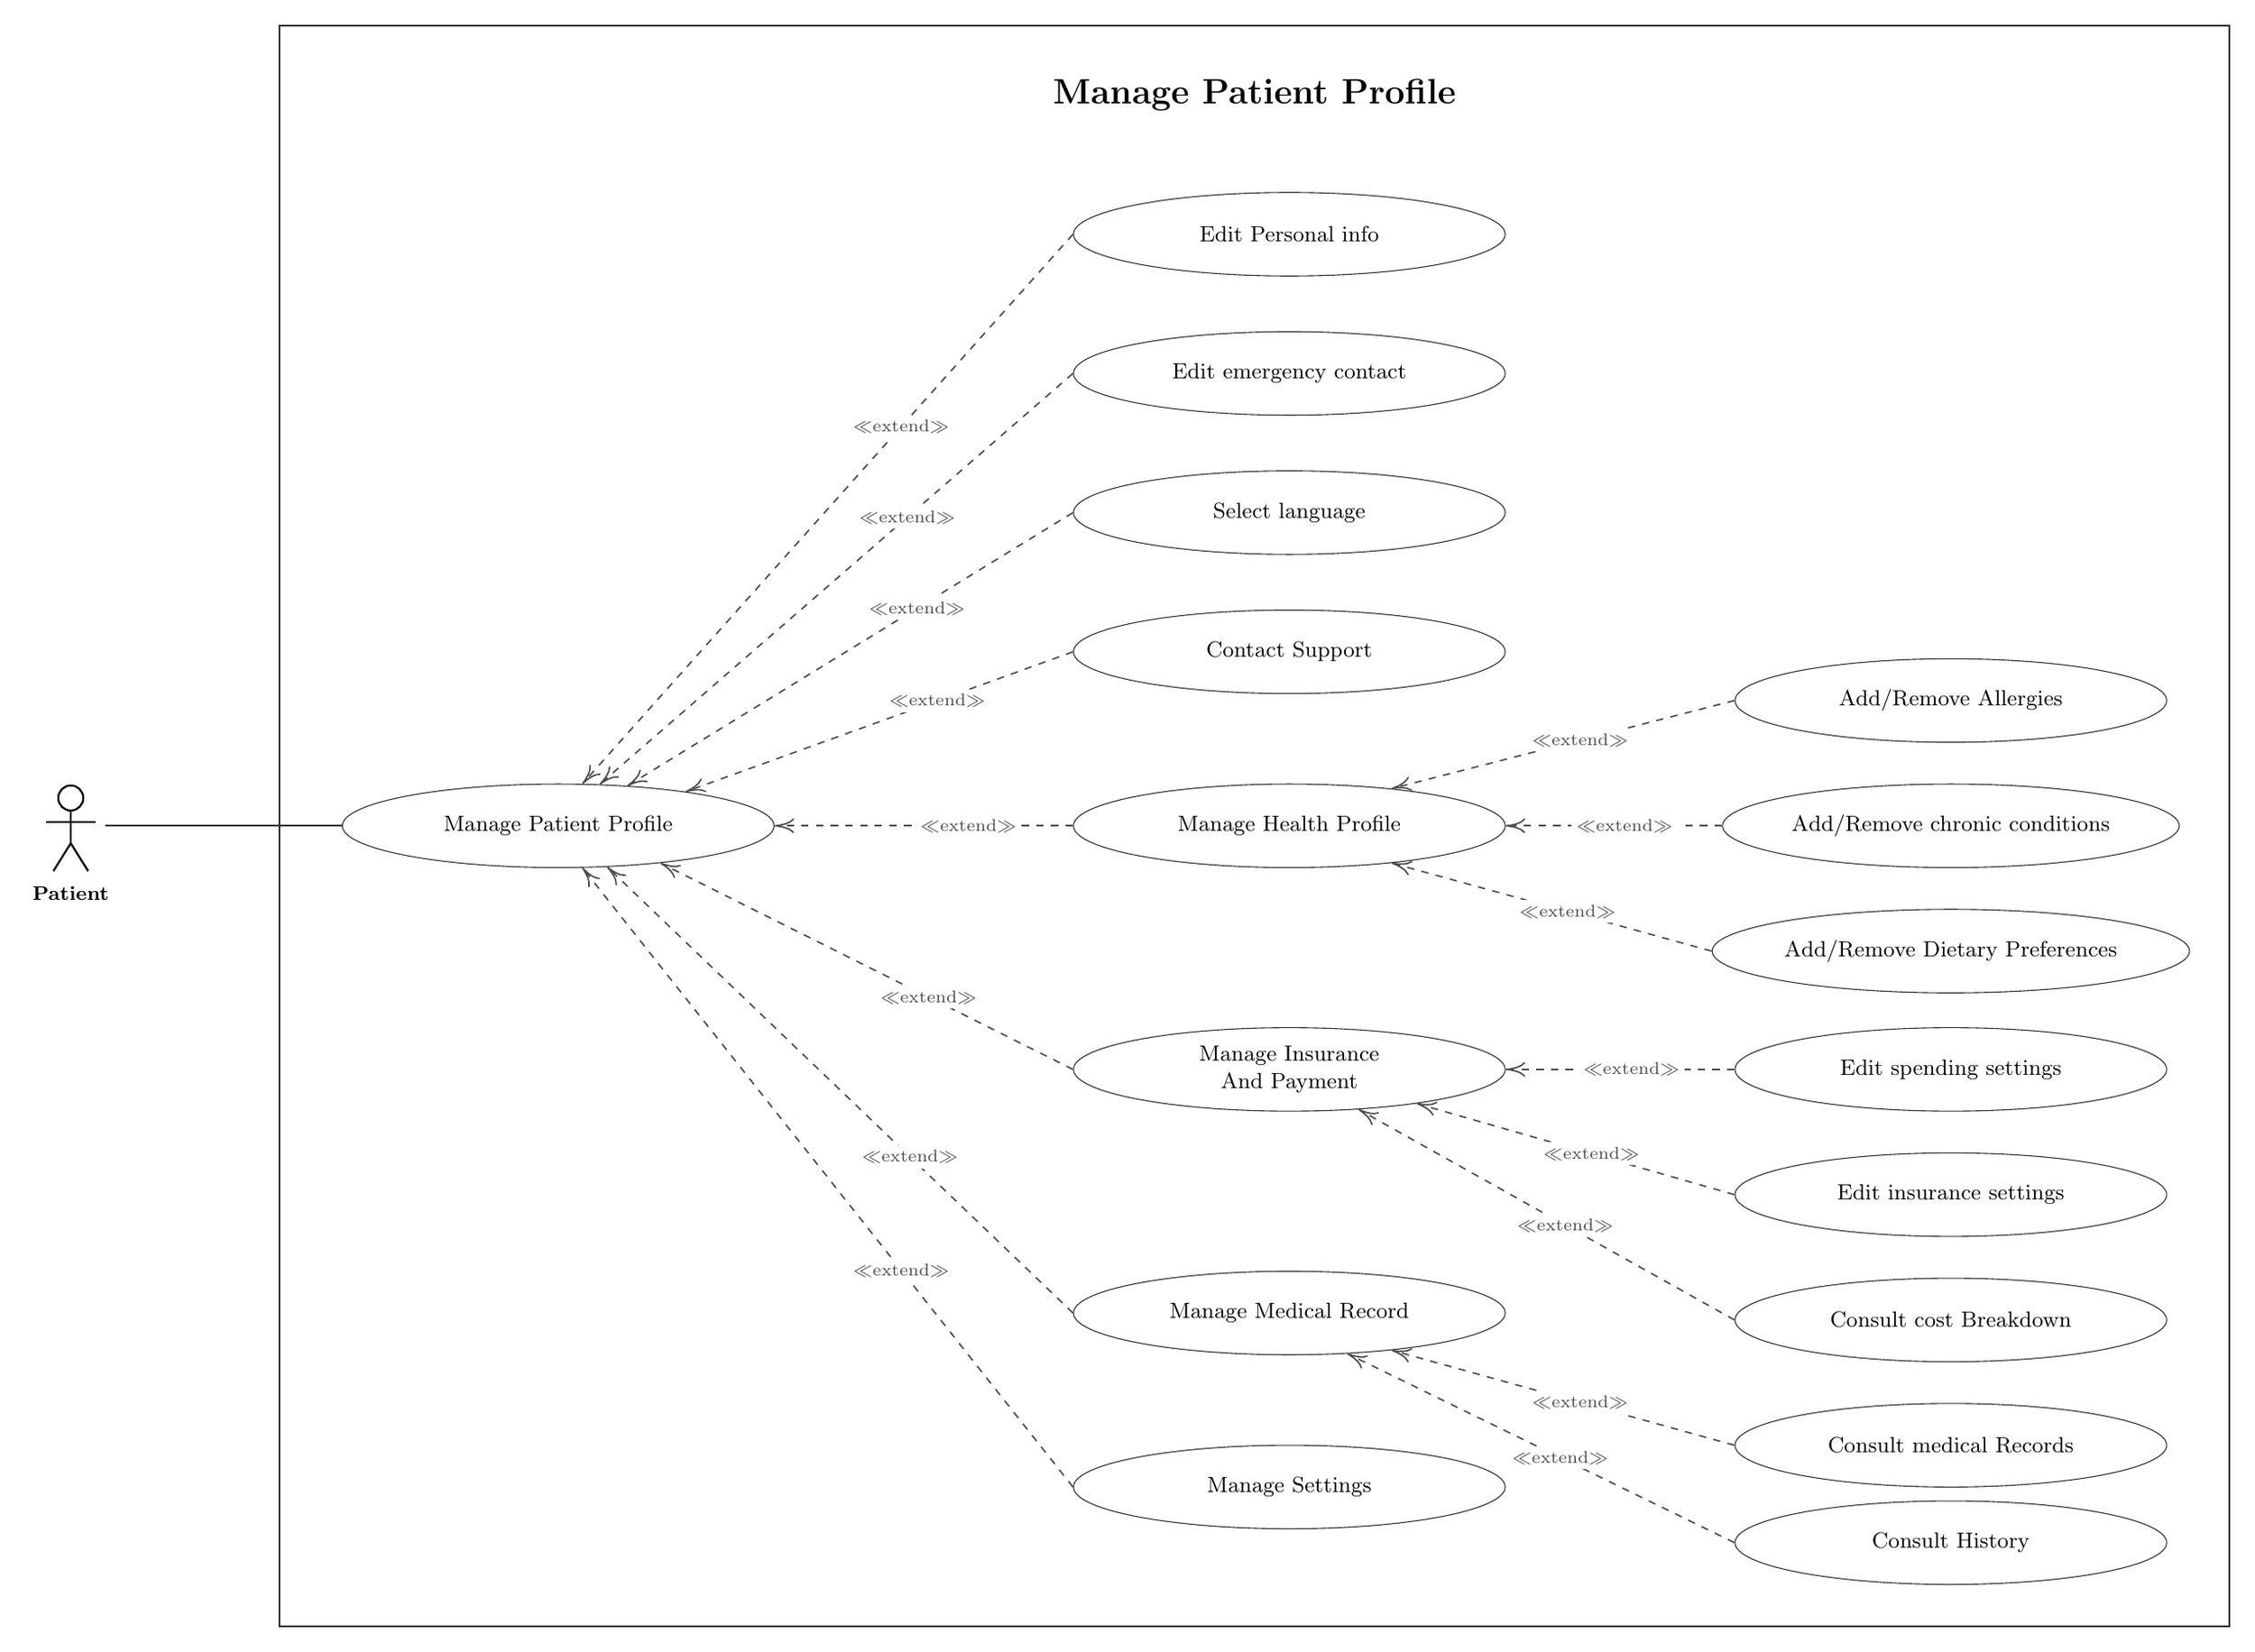
\begin{tikzpicture}[x=1cm,y=1cm]

% --- STYLES ---
\tikzset{
  actorlabel/.style={font=\footnotesize\bfseries, align=center},
  usecase/.style={ellipse, draw=black!80, fill=white,
                  font=\small, align=center,
                  minimum width=6.2cm, minimum height=1.2cm, inner sep=1pt},
  boundary/.style={draw=black!80, line width=0.8pt},
  assoc/.style={black!80, line width=0.6pt},
  extend/.style={black!70, dashed, line width=0.6pt,
                  -{>[length=8pt, width=6pt]}},
}

% --- ACTOR DRAWING MACRO ---
\newcommand{\actor}[3]{
  \begin{scope}[shift={(#1,#2)}]
    \draw[thick] (0,0.40) circle (0.18);
    \draw[thick] (0,0.22) -- (0,-0.25);
    \draw[thick] (-0.35,0.05) -- (0.35,0.05);
    \draw[thick] (0,-0.25) -- (-0.25,-0.65);
    \draw[thick] (0,-0.25) -- (0.25,-0.65);
    \node[actorlabel, below] at (0,-0.75) {#3};
  \end{scope}
}

% ================= EXPLICIT SYSTEM BOUNDARY & TITLE =================
\draw[boundary] (-0.5, 9.5) rectangle (27.5, -13.5);
\node[font=\Large\bfseries] at (13.5, 8.5) {Manage Patient Profile};

% ================= ACTOR =================
\actor{-3.5}{ -2.0}{Patient}

% ================= LEVEL 1: ROOT USE CASE =================
\node[usecase] (u1) at (3.5, -2.0) {Manage Patient Profile};
\draw[assoc] (-3.0, -2.0) -- (u1.west);

% ================= LEVEL 2: MAIN EXTENSIONS =================
\node[usecase] (e1a) at (14.0,  6.5) {Edit Personal info};
\node[usecase] (e1b) at (14.0,  4.5) {Edit emergency contact};
\node[usecase] (e1c) at (14.0,  2.5) {Select language};
\node[usecase] (e1d) at (14.0,  0.5) {Contact Support};

\node[usecase] (u2)  at (14.0, -2.0) {Manage Health Profile};
\node[usecase] (u3)  at (14.0, -5.5) {Manage Insurance \\ And Payment};
\node[usecase] (u4)  at (14.0, -9.0) {Manage Medical Record};
\node[usecase] (u5)  at (14.0,-11.5) {Manage Settings};

% ================= LEVEL 3: SUB-EXTENSIONS =================
\node[usecase] (e2a) at (23.5, -0.2) {Add/Remove Allergies};
\node[usecase] (e2b) at (23.5, -2.0) {Add/Remove chronic conditions};
\node[usecase] (e2c) at (23.5, -3.8) {Add/Remove Dietary Preferences};

\node[usecase] (e3a) at (23.5, -5.5) {Edit spending settings};
\node[usecase] (e3b) at (23.5, -7.3) {Edit insurance settings};
\node[usecase] (e3c) at (23.5, -9.1) {Consult cost Breakdown};

\node[usecase] (e4a) at (23.5,-10.9) {Consult medical Records};
\node[usecase] (e4b) at (23.5,-12.3) {Consult History};

% ================= STRICTLY STRAIGHT LINES =================
% --- From LEVEL 2 to LEVEL 1 ---
\draw[extend] (e1a.west) -- node[pos=0.35, fill=white, inner sep=2pt, font=\scriptsize] {$\ll$extend$\gg$} (u1.60);
\draw[extend] (e1b.west) -- node[pos=0.35, fill=white, inner sep=2pt, font=\scriptsize] {$\ll$extend$\gg$} (u1.45);
\draw[extend] (e1c.west) -- node[pos=0.35, fill=white, inner sep=2pt, font=\scriptsize] {$\ll$extend$\gg$} (u1.30);
\draw[extend] (e1d.west) -- node[pos=0.35, fill=white, inner sep=2pt, font=\scriptsize] {$\ll$extend$\gg$} (u1.15);
\draw[extend] (u2.west)  -- node[pos=0.35, fill=white, inner sep=2pt, font=\scriptsize] {$\ll$extend$\gg$} (u1.0);
\draw[extend] (u3.west)  -- node[pos=0.35, fill=white, inner sep=2pt, font=\scriptsize] {$\ll$extend$\gg$} (u1.-20);
\draw[extend] (u4.west)  -- node[pos=0.35, fill=white, inner sep=2pt, font=\scriptsize] {$\ll$extend$\gg$} (u1.-40);
\draw[extend] (u5.west)  -- node[pos=0.35, fill=white, inner sep=2pt, font=\scriptsize] {$\ll$extend$\gg$} (u1.-60);

% --- From LEVEL 3 to LEVEL 2 ---
\draw[extend] (e2a.west) -- node[pos=0.45, fill=white, inner sep=2pt, font=\scriptsize] {$\ll$extend$\gg$} (u2.20);
\draw[extend] (e2b.west) -- node[pos=0.45, fill=white, inner sep=2pt, font=\scriptsize] {$\ll$extend$\gg$} (u2.0);
\draw[extend] (e2c.west) -- node[pos=0.45, fill=white, inner sep=2pt, font=\scriptsize] {$\ll$extend$\gg$} (u2.-20);

\draw[extend] (e3a.west) -- node[pos=0.45, fill=white, inner sep=2pt, font=\scriptsize] {$\ll$extend$\gg$} (u3.0);
\draw[extend] (e3b.west) -- node[pos=0.45, fill=white, inner sep=2pt, font=\scriptsize] {$\ll$extend$\gg$} (u3.-15);
\draw[extend] (e3c.west) -- node[pos=0.45, fill=white, inner sep=2pt, font=\scriptsize] {$\ll$extend$\gg$} (u3.-30);

\draw[extend] (e4a.west) -- node[pos=0.45, fill=white, inner sep=2pt, font=\scriptsize] {$\ll$extend$\gg$} (u4.-20);
\draw[extend] (e4b.west) -- node[pos=0.45, fill=white, inner sep=2pt, font=\scriptsize] {$\ll$extend$\gg$} (u4.-35);

\end{tikzpicture}
}}
    \caption{Refined Use Case Diagram: Manage Patient Profile}
    \label{fig:uc patient detail}
\end{figure}

\begin{table}[H]
\centering
\caption{Use Case Description: ``Manage Patient Profile''}
\label{tab:uc patient detail}
\small
\begin{tabular}{|l|p{10cm}|}
\hline
\textbf{Use Case} & Manage Patient Profile \\
\hline
\textbf{Primary Actor} & Patient \\
\hline
\textbf{Preconditions} & Patient authenticated \\
\hline
\textbf{Postconditions} & Profile information and preferences updated in the database \\
\hline
\textbf{Main Scenario} &
\begin{minipage}[t]{9.5cm}
\vspace{2pt}
1. The patient navigates to the Profile section from the main menu\\
2. The system retrieves and displays current profile data (personal info, emergency contact, health profile, insurance, app settings)\\
3. The patient selects a section to edit (Personal Info, Emergency Contact, Health Profile, Insurance, App Settings, or Profile Photo)\\
4. The patient modifies the desired fields in the selected section\\
5. The patient optionally uploads or updates a profile photo\\
6. The patient taps the Save button\\
7. The system validates all modified fields (required fields, format constraints, data consistency)\\
8. The system persists the changes to the database\\
9. The system displays a success confirmation message\\
10. The system refreshes the displayed profile with the updated data
\vspace{2pt}
\end{minipage} \\
\hline
\textbf{Alternative Flows} &
\begin{minipage}[t]{9.5cm}
\vspace{2pt}
4a. Invalid input data: The system highlights the erroneous fields and shows specific validation messages. The patient corrects the inputs and resubmits.\\
6a. Cancel changes: The patient discards changes at any point. The system reverts to the previously saved profile data without confirmation.\\
6b. Network error during save: The system detects a connection failure, retains the unsaved changes locally, and prompts the patient to retry or save for later.\\
5a. Upload photo failure: The selected image exceeds the allowed size or format. The system notifies the patient with the accepted requirements and allows reselection.\\
Session timeout: The patient's session expires during editing. The system redirects to the login page. Unsaved changes are lost.
\vspace{2pt}
\end{minipage} \\
\hline
\end{tabular}
\end{table}

\subsubsection{Consult Patient Dashboard}

This refined use case illustrates the main features available from the patient dashboard, including the recovery index, risk score, insights, services management, medication management, and AI assistant interaction.

\includepdf[fitpaper=true, pages=-, pagecommand={}]{uc-patient-dashboard-a3.pdf}

\begin{table}[H]
\centering
\caption{Use Case Description: ``Consult Patient Dashboard''}
\label{tab:uc patient dashboard}
\small
\begin{tabular}{|l|p{10cm}|}
\hline
\textbf{Use Case} & Consult Patient Dashboard \\
\hline
\textbf{Primary Actor} & Patient \\
\hline
\textbf{Preconditions} & Patient authenticated \\
\hline
\textbf{Postconditions} & Dashboard data displayed; managed services, medications, and AI interactions recorded \\
\hline
\textbf{Main Scenario} &
\begin{minipage}[t]{9.5cm}
\vspace{2pt}
1. The patient opens the dashboard\\
2. The system loads the schedule, recovery index, health insights, and risk score\\
3. The patient manages health services (records sleep data, logs physical activity, uploads lab results, consults follow up plan)\\
4. The patient manages medications (adds a new medication, consults current medications, marks medications as taken)\\
5. The patient interacts with the AI health assistant for conversational guidance\\
6. The system refreshes the dashboard indicators and AI driven insights accordingly
\vspace{2pt}
\end{minipage} \\
\hline
\textbf{Alternative Flows} &
\begin{minipage}[t]{9.5cm}
\vspace{2pt}
3a. Invalid service data: The system rejects invalid inputs (e.g., unrealistic sleep hours, malformed lab file) and prompts the patient to correct them.\\
4a. Medication conflict: The system detects a duplicate or conflicting medication entry and notifies the patient before adding.\\
4b. Mark medication as missed: The patient can mark a medication as missed instead of taken; the system logs the adherence gap.\\
5a. AI assistant unavailable: The system displays a message indicating the AI service is temporarily unavailable and offers manual navigation.\\
Network error: The system shows an error state with a retry option; any locally entered data is preserved.
\vspace{2pt}
\end{minipage} \\
\hline
\end{tabular}
\end{table}

\subsubsection{Consult Doctor Dashboard}

This refined use case presents how a doctor consults their dashboard to access the schedule, risk radar, critical alerts, and to interact with clinical AI tools for decision support.

\begin{figure}[H]
    \centering
\rotatebox{90}{\resizebox{0.9\textheight}{!}{% Consult Doctor Dashboard Use Case Diagram
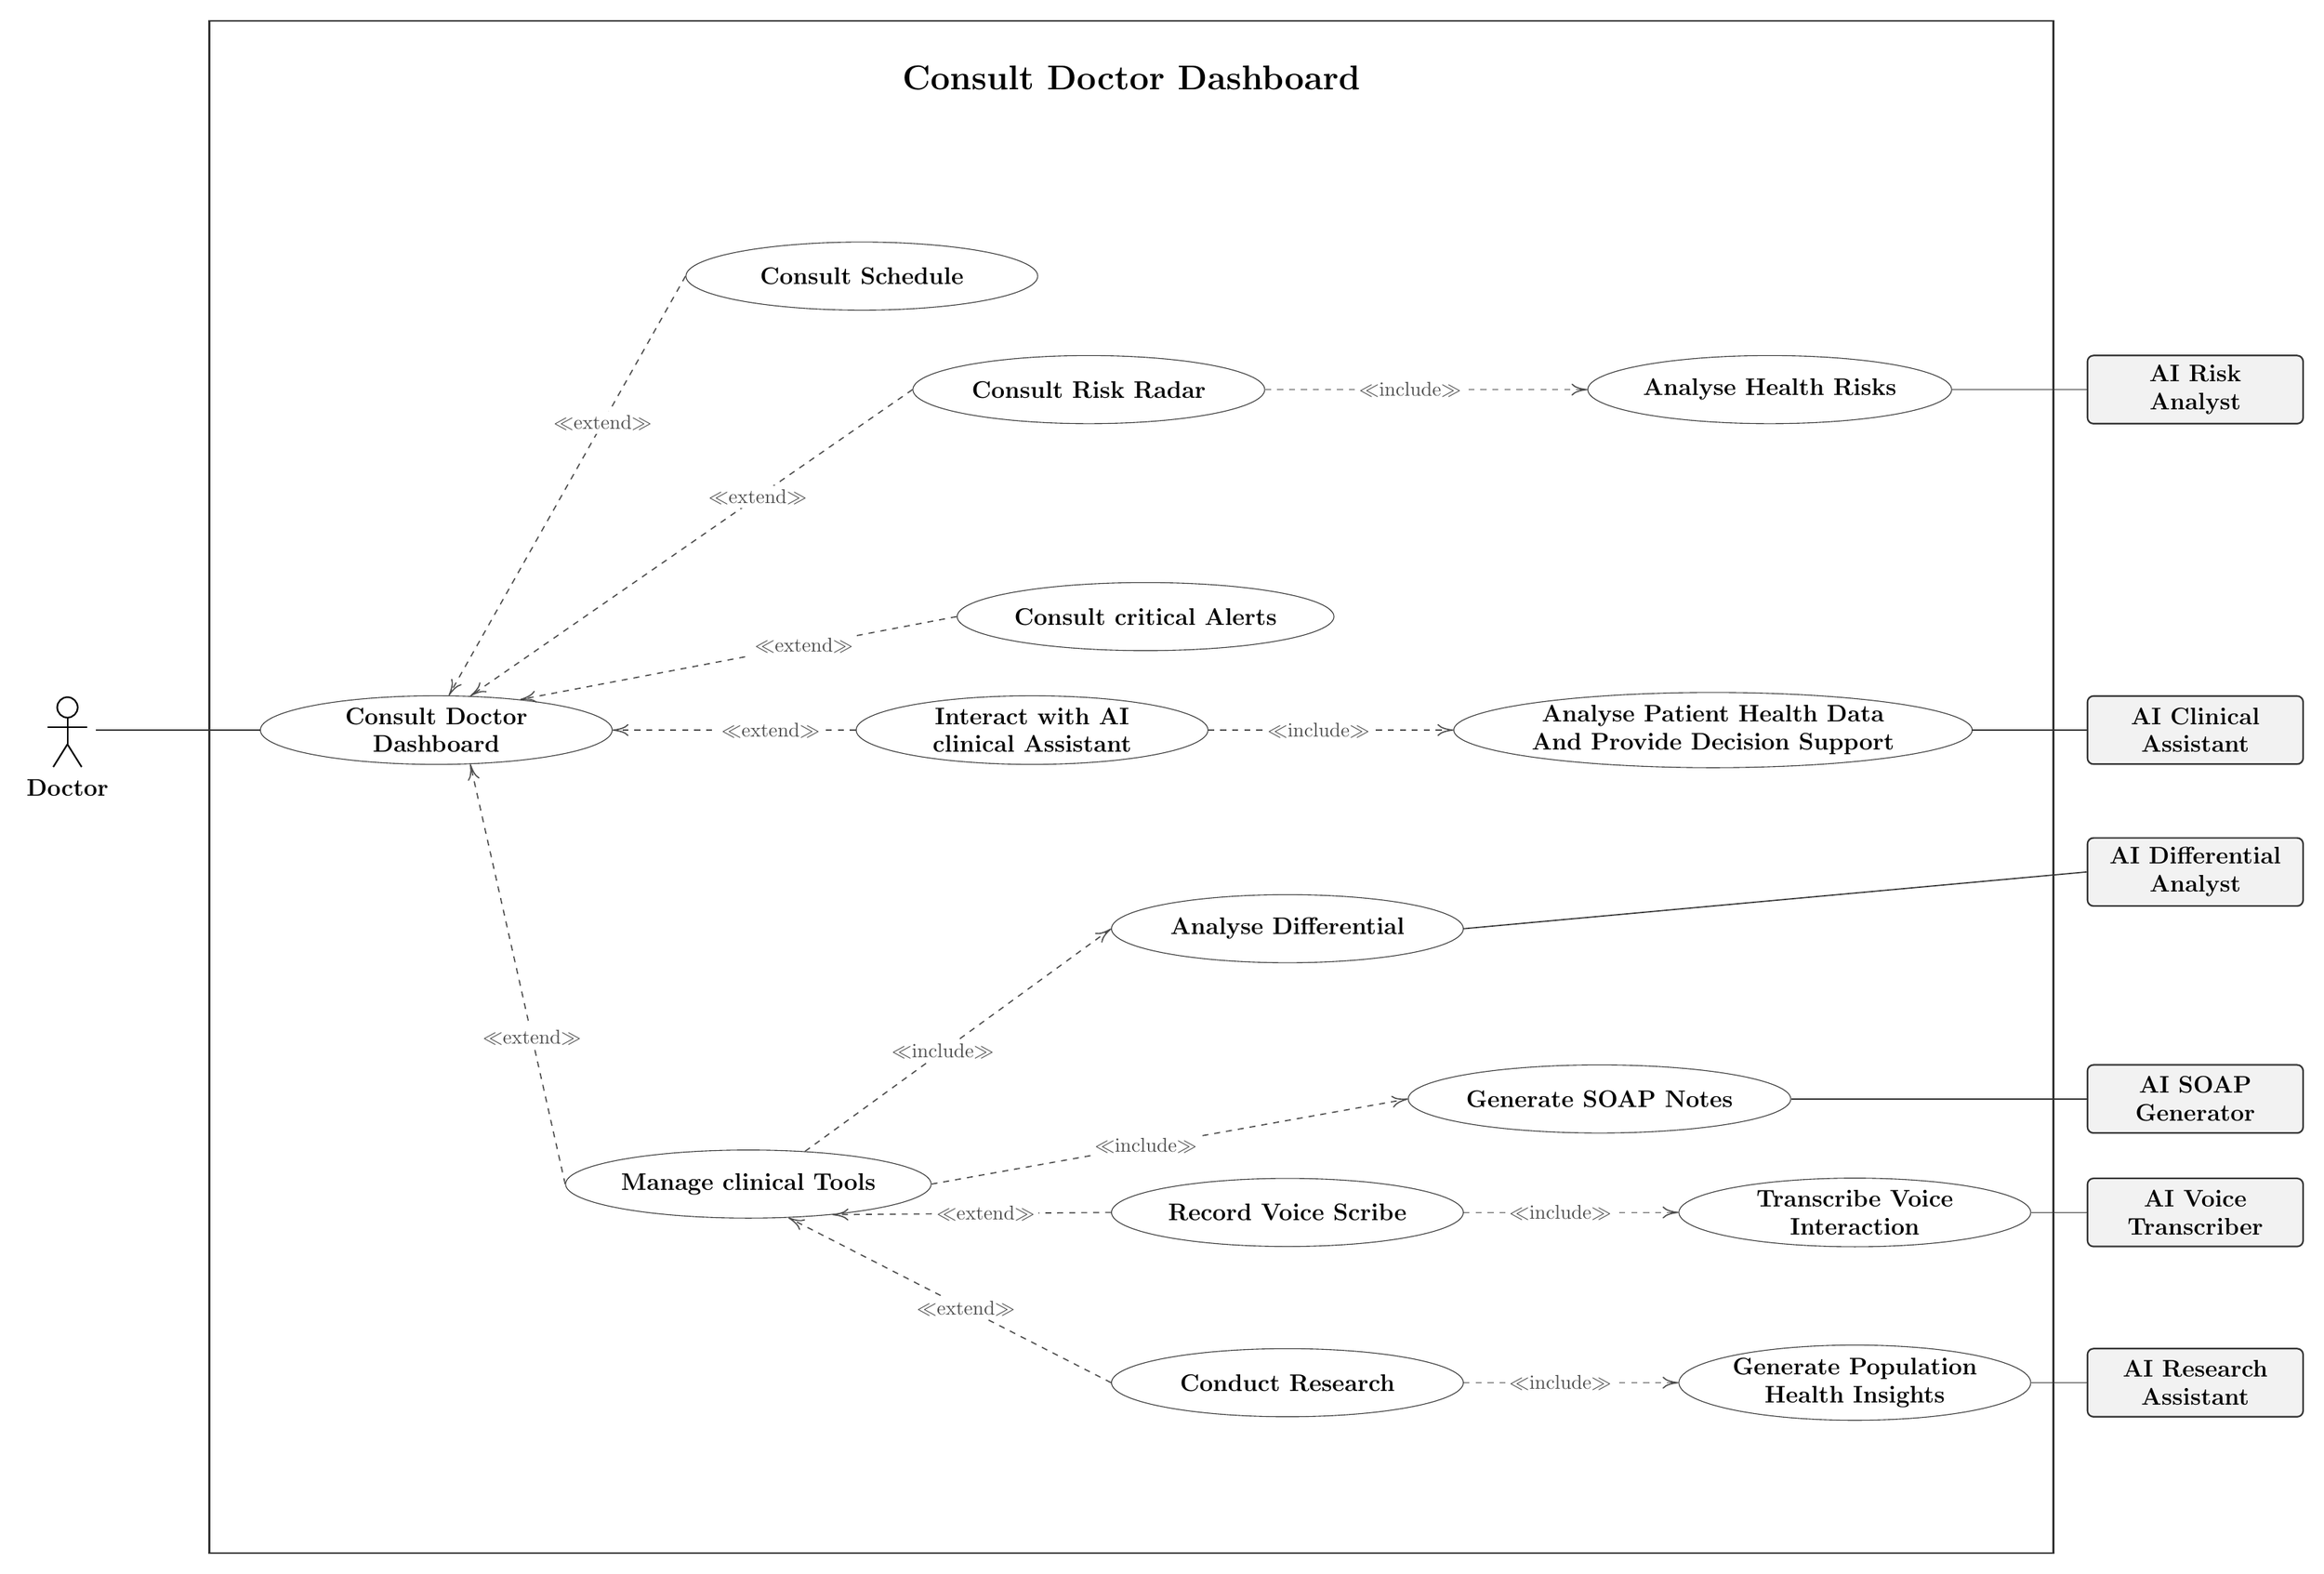
\begin{tikzpicture}[x=1cm,y=1cm]

\tikzset{
  actorlabel/.style={font=\large\bfseries, align=center},
  usecase/.style={ellipse, draw=black!80, fill=white,
                  font=\large\bfseries, align=center,
                  minimum width=6.2cm, minimum height=1.2cm, inner sep=1pt},
  boundary/.style={draw=black!80, line width=0.8pt},
  assoc/.style={black!80, line width=0.6pt},
  extend/.style={black!70, dashed, line width=0.6pt,
                  -{>[length=8pt, width=6pt]}},
  systemactor/.style={rectangle, draw=black!80, thick, fill=gray!10,
                  font=\large\bfseries, align=center,
                  minimum width=3.8cm, minimum height=1.2cm, rounded corners=3pt}
}

\newcommand{\actor}[3]{
  \begin{scope}[shift={(#1,#2)}]
    \draw[thick] (0,0.40) circle (0.18);
    \draw[thick] (0,0.22) -- (0,-0.25);
    \draw[thick] (-0.35,0.05) -- (0.35,0.05);
    \draw[thick] (0,-0.25) -- (-0.25,-0.65);
    \draw[thick] (0,-0.25) -- (0.25,-0.65);
    \node[actorlabel, below] at (0,-0.75) {#3};
  \end{scope}
}

% Boundary and title
\draw[boundary] (-0.5, 13.5) rectangle (32.0, -13.5);
\node[font=\LARGE\bfseries] at (15.75, 12.5) {Consult Doctor Dashboard};

% Actors
\actor{-3.0}{1.0}{Doctor}

% AI actors
\node[systemactor] (airisk) at (34.5,  7.0) {AI Risk\\Analyst};
\node[systemactor] (aiclin) at (34.5,  1.0) {AI Clinical\\Assistant};
\node[systemactor] (aidiff) at (34.5, -1.5) {AI Differential\\Analyst};
\node[systemactor] (aisoap) at (34.5, -5.5) {AI SOAP\\Generator};
\node[systemactor] (aivoice) at (34.5, -7.5) {AI Voice\\Transcriber};
\node[systemactor] (aires)  at (34.5, -10.5) {AI Research\\Assistant};

% Root
\node[usecase] (dash) at (3.5, 1.0) {Consult Doctor\\Dashboard};
\draw[assoc] (-2.5, 1.0) -- (dash.west);

% Level 2
\node[usecase] (sched)    at (11.0,  9.0) {Consult Schedule};
\node[usecase] (risk)     at (15.0,  7.0) {Consult Risk Radar};
\node[usecase] (alerts)   at (16.0,  3.0) {Consult critical Alerts};
\node[usecase] (interact) at (14.0,  1.0) {Interact with AI\\clinical Assistant};
\node[usecase] (tools)    at ( 9.0, -7.0) {Manage clinical Tools};

% Level 3
\node[usecase] (arisks)   at (27.0,  7.0) {Analyse Health Risks};
\node[usecase] (apat)     at (26.0,  1.0) {Analyse Patient Health Data\\And Provide Decision Support};
\node[usecase] (soap)     at (24.0, -5.5) {Generate SOAP Notes};

\node[usecase] (diff)     at (18.5, -2.5) {Analyse Differential};
\node[usecase] (voice)    at (18.5, -7.5) {Record Voice Scribe};
\node[usecase] (research) at (18.5, -10.5) {Conduct Research};

% Level 4
\node[usecase] (trans)    at (28.5, -7.5) {Transcribe Voice\\Interaction};
\node[usecase] (insight)  at (28.5, -10.5) {Generate Population\\Health Insights};

% Lines
\draw[extend] (sched.west)    -- node[pos=0.35, fill=white, inner sep=2pt, font=\normalsize] {$\ll$extend$\gg$} (dash.70);
\draw[extend] (risk.west)     -- node[pos=0.35, fill=white, inner sep=2pt, font=\normalsize] {$\ll$extend$\gg$} (dash.45);
\draw[extend] (alerts.west)   -- node[pos=0.35, fill=white, inner sep=2pt, font=\normalsize] {$\ll$extend$\gg$} (dash.20);
\draw[extend] (interact.west) -- node[pos=0.35, fill=white, inner sep=2pt, font=\normalsize] {$\ll$extend$\gg$} (dash.0);
\draw[extend] (tools.west)    -- node[pos=0.35, fill=white, inner sep=2pt, font=\normalsize] {$\ll$extend$\gg$} (dash.-45);

\draw[extend] (risk.east)     -- node[pos=0.45, fill=white, inner sep=2pt, font=\normalsize] {$\ll$include$\gg$} (arisks.west);
\draw[extend] (interact.east) -- node[pos=0.45, fill=white, inner sep=2pt, font=\normalsize] {$\ll$include$\gg$} (apat.west);

\draw[extend] (tools.30)     -- node[pos=0.45, fill=white, inner sep=2pt, font=\normalsize] {$\ll$include$\gg$} (diff.west);
\draw[extend] (tools.0)     -- node[pos=0.45, fill=white, inner sep=2pt, font=\normalsize] {$\ll$include$\gg$} (soap.west);
\draw[extend] (voice.west)    -- node[pos=0.45, fill=white, inner sep=2pt, font=\normalsize] {$\ll$extend$\gg$} (tools.-20);
\draw[extend] (research.west) -- node[pos=0.45, fill=white, inner sep=2pt, font=\normalsize] {$\ll$extend$\gg$} (tools.-40);

\draw[extend] (voice.east)    -- node[pos=0.45, fill=white, inner sep=2pt, font=\normalsize] {$\ll$include$\gg$} (trans.west);
\draw[extend] (research.east) -- node[pos=0.45, fill=white, inner sep=2pt, font=\normalsize] {$\ll$include$\gg$} (insight.west);

% Associations
\draw[assoc] (arisks.east)  -- (airisk.west);
\draw[assoc] (apat.east)    -- (aiclin.west);
\draw[assoc] (diff.east)    -- (aidiff.west);
\draw[assoc] (soap.east)    -- (aisoap.west);
\draw[assoc] (trans.east)   -- (aivoice.west);
\draw[assoc] (insight.east) -- (aires.west);

\end{tikzpicture}
}}
    \caption{Refined Use Case Diagram: Consult Doctor Dashboard}
    \label{fig:uc doctor dashboard}
\end{figure}

\begin{table}[H]
\centering
\caption{Use Case Description: ``Consult Doctor Dashboard''}
\label{tab:uc doctor dashboard}
\small
\begin{tabular}{|l|p{10cm}|}
\hline
\textbf{Use Case} & Consult Doctor Dashboard \\
\hline
\textbf{Primary Actor} & Doctor \\
\hline
\textbf{Preconditions} & Doctor authenticated; at least one patient linked \\
\hline
\textbf{Postconditions} & Dashboard data displayed; clinical AI analyses generated and available for review \\
\hline
\textbf{Main Scenario} &
\begin{minipage}[t]{9.5cm}
\vspace{2pt}
1. The doctor opens the dashboard\\
2. The system displays the schedule, critical alerts, and clinical tool shortcuts\\
3. The doctor reviews the risk radar for highlighted patients\\
4. The doctor manages clinical tools (analyses differential diagnosis, generates SOAP notes, records a voice scribe, conducts research)\\
5. The doctor interacts with the AI clinical assistant for decision support on a selected patient\\
6. The system updates the dashboard with AI generated results and recommendations
\vspace{2pt}
\end{minipage} \\
\hline
\textbf{Alternative Flows} &
\begin{minipage}[t]{9.5cm}
\vspace{2pt}
4a. AI analysis unavailable: The system displays a warning that the AI service is offline and allows the doctor to proceed with manual workflows.\\
4b. Incomplete patient data: The system notifies the doctor that insufficient data is available for a reliable analysis and suggests completing the patient record first.\\
3a. No critical alerts: The system shows an empty state for alerts; the doctor proceeds to access clinical tools directly.\\
5a. Patient not selected: The doctor must select a patient before accessing AI decision support; the system prompts for selection.\\
Network error: The system displays an error state and allows retry; previously loaded data remains visible.
\vspace{2pt}
\end{minipage} \\
\hline
\end{tabular}
\end{table}

\subsubsection{Manage Doctor Profile}

This refined use case describes how a doctor manages their professional profile, including schedule and fees, language preferences, reviews, revenue overview, and support options.

\begin{figure}[H]
    \centering
    \rotatebox{90}{\resizebox{0.9\textheight}{!}{% Complete Doctor Profile Use Case Diagram
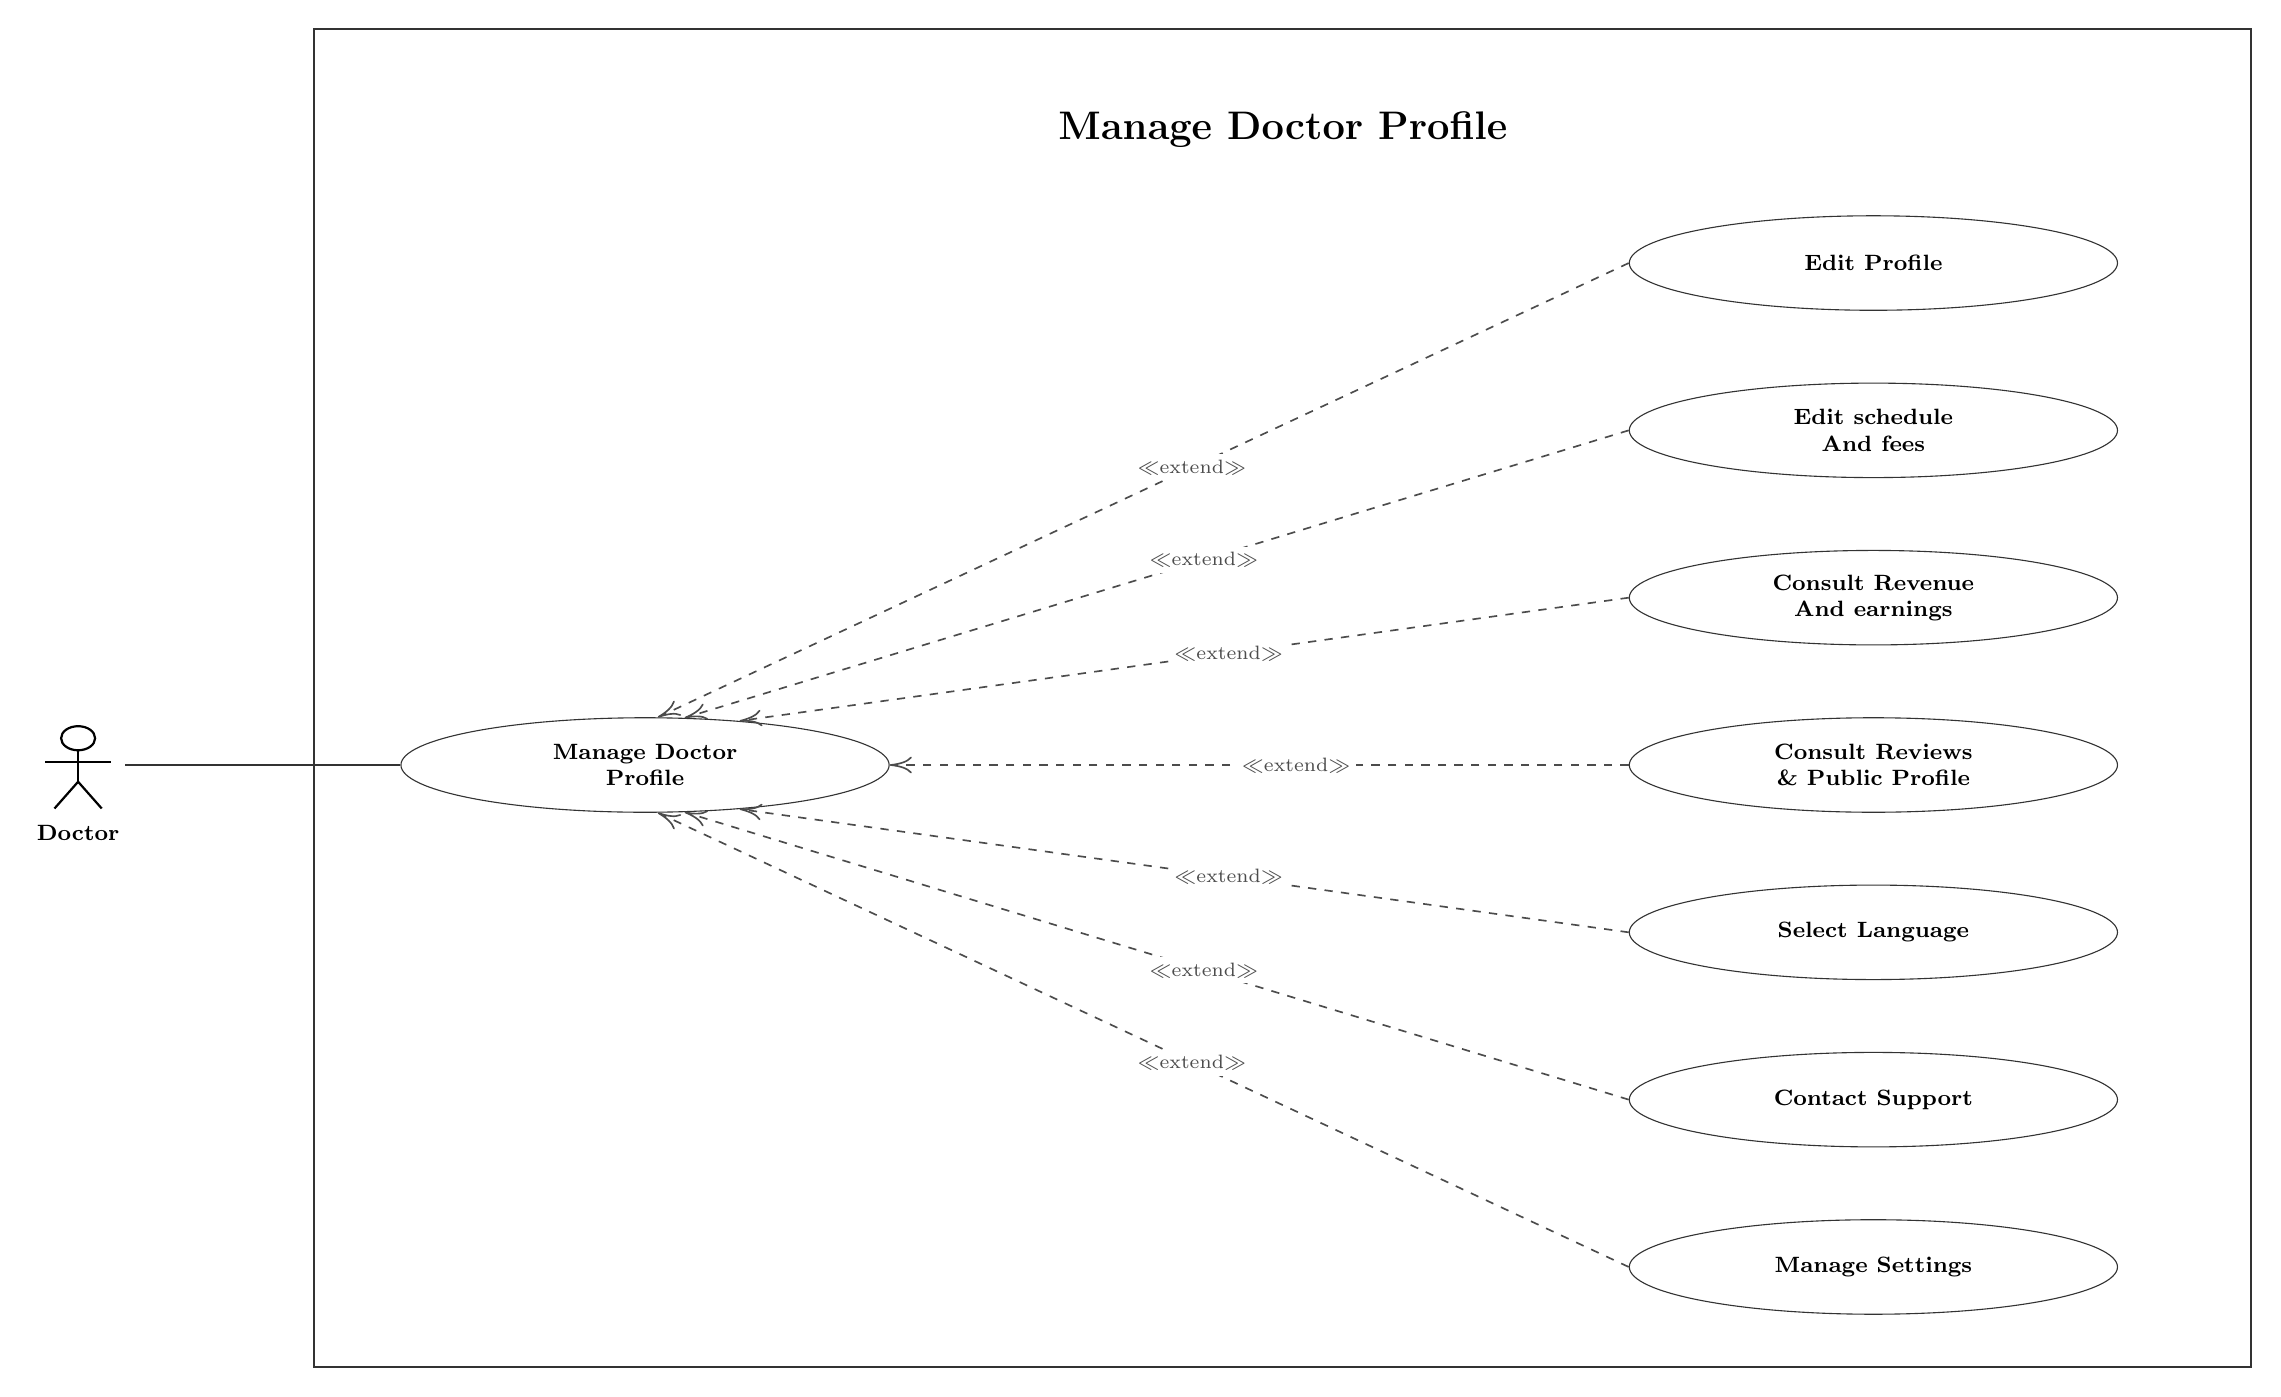
\begin{tikzpicture}[x=1.2cm,y=0.85cm]

\tikzset{
  actorlabel/.style={font=\footnotesize\bfseries, align=center},
  usecase/.style={ellipse, draw=black!80, fill=white,
                  font=\footnotesize\bfseries, align=center,
                  minimum width=6.2cm, minimum height=1.2cm, inner sep=1pt},
  boundary/.style={draw=black!80, line width=0.8pt},
  assoc/.style={black!80, line width=0.6pt},
  extend/.style={black!70, dashed, line width=0.6pt,
                  -{>[length=8pt, width=6pt]}}
}

\newcommand{\actor}[3]{
  \begin{scope}[shift={(#1,#2)}]
    \draw[thick] (0,0.40) circle (0.18);
    \draw[thick] (0,0.22) -- (0,-0.25);
    \draw[thick] (-0.35,0.05) -- (0.35,0.05);
    \draw[thick] (0,-0.25) -- (-0.25,-0.65);
    \draw[thick] (0,-0.25) -- (0.25,-0.65);
    \node[actorlabel, below] at (0,-0.75) {#3};
  \end{scope}
}

% Boundary and title
\draw[boundary] (-0.5, 11.0) rectangle (20.0, -9.0);
\node[font=\Large\bfseries] at (9.75, 9.5) {Manage Doctor Profile};

% Actor
\actor{-3.0}{0.0}{Doctor}

% Root
\node[usecase] (root) at (3.0, 0.0) {Manage Doctor\\Profile};
\draw[assoc] (-2.5, 0.0) -- (root.west);

% Extensions
\node[usecase] (uc1) at (16.0,  7.5) {Edit Profile};
\node[usecase] (uc2) at (16.0,  5.0) {Edit schedule\\And fees};
\node[usecase] (uc3) at (16.0,  2.5) {Consult Revenue\\And earnings};
\node[usecase] (uc4) at (16.0,  0.0) {Consult Reviews\\\& Public Profile};
\node[usecase] (uc5) at (16.0, -2.5) {Select Language};
\node[usecase] (uc6) at (16.0, -5.0) {Contact Support};
\node[usecase] (uc7) at (16.0, -7.5) {Manage Settings};

% Lines
\draw[extend] (uc1.west) -- node[pos=0.45, fill=white, inner sep=2pt, font=\scriptsize] {$\ll$extend$\gg$} (root.75);
\draw[extend] (uc2.west) -- node[pos=0.45, fill=white, inner sep=2pt, font=\scriptsize] {$\ll$extend$\gg$} (root.50);
\draw[extend] (uc3.west) -- node[pos=0.45, fill=white, inner sep=2pt, font=\scriptsize] {$\ll$extend$\gg$} (root.25);
\draw[extend] (uc4.west) -- node[pos=0.45, fill=white, inner sep=2pt, font=\scriptsize] {$\ll$extend$\gg$} (root.0);
\draw[extend] (uc5.west) -- node[pos=0.45, fill=white, inner sep=2pt, font=\scriptsize] {$\ll$extend$\gg$} (root.-25);
\draw[extend] (uc6.west) -- node[pos=0.45, fill=white, inner sep=2pt, font=\scriptsize] {$\ll$extend$\gg$} (root.-50);
\draw[extend] (uc7.west) -- node[pos=0.45, fill=white, inner sep=2pt, font=\scriptsize] {$\ll$extend$\gg$} (root.-75);

\end{tikzpicture}
}}
    \caption{Refined Use Case Diagram: Manage Doctor Profile}
    \label{fig:uc doctor profile}
\end{figure}

\begin{table}[H]
\centering
\caption{Use Case Description: ``Manage Doctor Profile''}
\label{tab:uc doctor profile}
\small
\begin{tabular}{|l|p{10cm}|}
\hline
\textbf{Use Case} & Manage Doctor Profile \\
\hline
\textbf{Primary Actor} & Doctor \\
\hline
\textbf{Preconditions} & Doctor authenticated \\
\hline
\textbf{Postconditions} & Profile, schedule, fees, and preferences updated in the database \\
\hline
\textbf{Main Scenario} &
\begin{minipage}[t]{9.5cm}
\vspace{2pt}
1. The doctor opens the profile section\\
2. The system retrieves and displays the current profile (personal info, schedule, fees, languages, reviews, revenue overview)\\
3. The doctor selects a section to edit (Personal Info, Schedule \& Fees, Languages, or Support)\\
4. The doctor updates the desired fields (e.g., changes availability slots, adjusts consultation fees, adds a language)\\
5. The doctor optionally updates the profile photo or bio\\
6. The doctor taps the Save button\\
7. The system validates the modified data (slot conflicts, fee formatting, required fields)\\
8. The system persists the changes to the database\\
9. The system displays a success confirmation\\
10. The system refreshes the displayed profile with the updated data
\vspace{2pt}
\end{minipage} \\
\hline
\textbf{Alternative Flows} &
\begin{minipage}[t]{9.5cm}
\vspace{2pt}
7a. Invalid schedule slot: The system detects overlapping or out of range time slots and highlights the conflict. The doctor adjusts the schedule and resubmits.\\
6a. Cancel changes: The doctor discards edits at any point. The system reverts to the previously saved profile data.\\
6b. Network error during save: The system detects a connection failure, retains unsaved changes locally, and prompts the doctor to retry or save for later.\\
Photo upload failure: The selected image exceeds the allowed size or format. The system notifies the doctor with the accepted requirements and allows reselection.\\
Session timeout: The doctor's session expires during editing. The system redirects to the login page. Unsaved changes are lost.
\vspace{2pt}
\end{minipage} \\
\hline
\end{tabular}
\end{table}

\subsubsection{Manage Doctors}

This refined use case details the administration workflow used to consult the doctors list and apply moderation actions such as approval, rejection, suspension, or deletion.

\begin{figure}[H]
    \centering
    \rotatebox{90}{\resizebox{0.9\textheight}{!}{% Admin - Manage Doctors Use Case Diagram
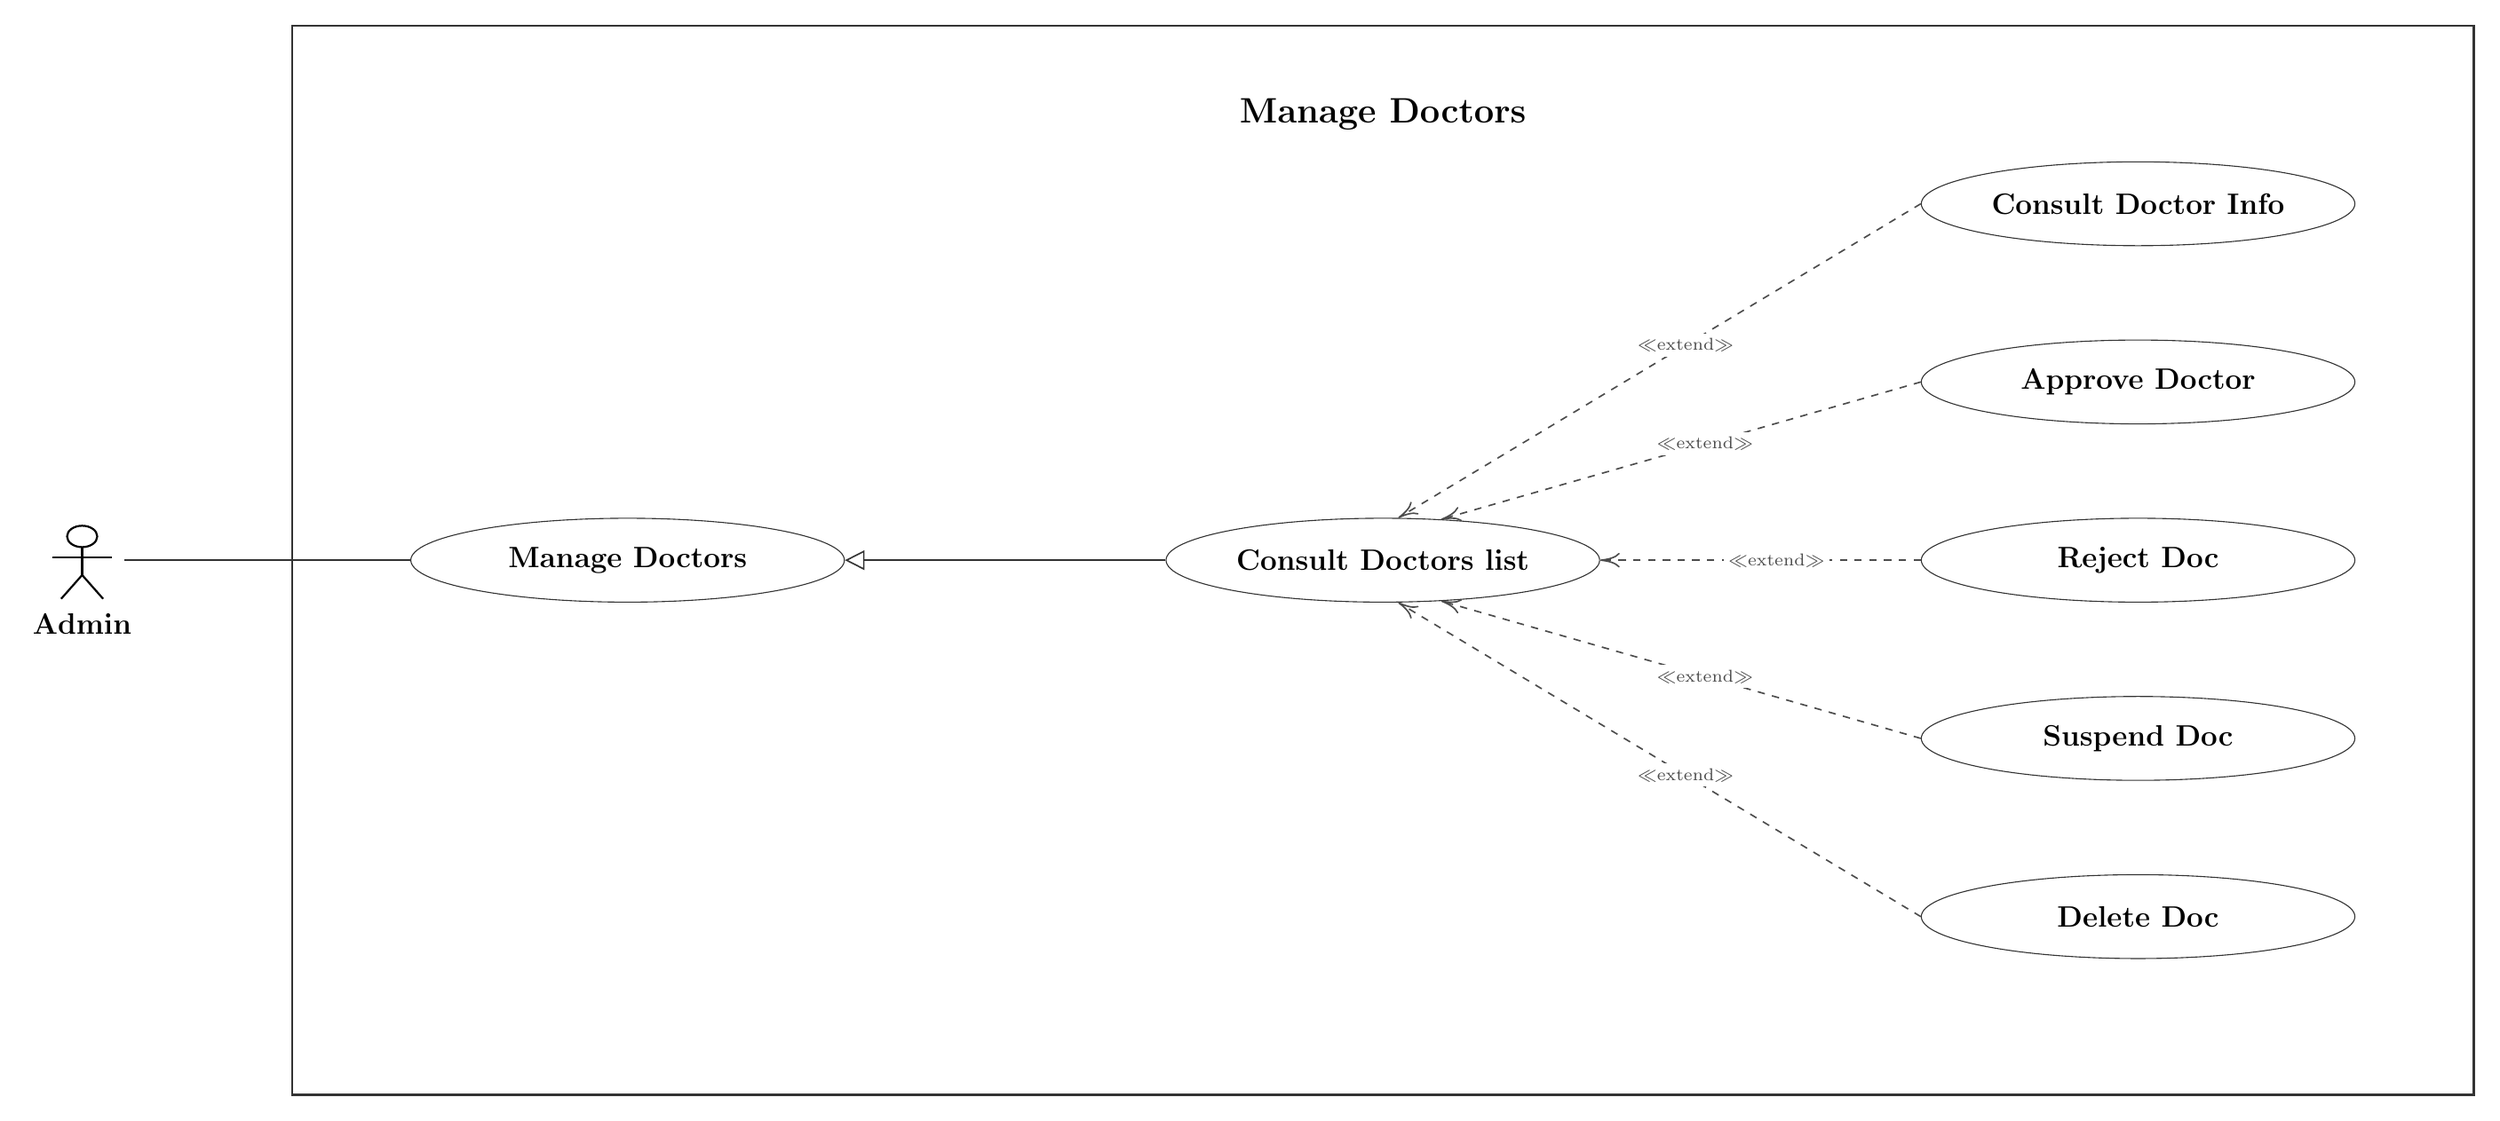
\begin{tikzpicture}[x=1.2cm,y=0.85cm]

\tikzset{
  actorlabel/.style={font=\large\bfseries, align=center},
  usecase/.style={ellipse, draw=black!80, fill=white,
                  font=\large\bfseries, align=center,
                  minimum width=6.2cm, minimum height=1.2cm, inner sep=1pt},
  boundary/.style={draw=black!80, line width=0.8pt},
  assoc/.style={black!80, line width=0.6pt},
  extend/.style={black!70, dashed, line width=0.6pt,
                  -{>[length=8pt, width=6pt]}},
  generalization/.style={black!80, line width=0.6pt,
                  -{Triangle[open, length=8pt, width=8pt]}}
}

\newcommand{\actor}[3]{
  \begin{scope}[shift={(#1,#2)}]
    \draw[thick] (0,0.40) circle (0.18);
    \draw[thick] (0,0.22) -- (0,-0.25);
    \draw[thick] (-0.35,0.05) -- (0.35,0.05);
    \draw[thick] (0,-0.25) -- (-0.25,-0.65);
    \draw[thick] (0,-0.25) -- (0.25,-0.65);
    \node[actorlabel, below] at (0,-0.75) {#3};
  \end{scope}
}

% Boundary and title
\draw[boundary] (-0.5, 9.0) rectangle (25.5, -9.0);
\node[font=\Large\bfseries] at (12.5, 7.5) {Manage Doctors};

% Actor
\actor{-3.0}{0.0}{Admin}

% Root
\node[usecase] (root) at (3.5, 0.0) {Manage Doctors};
\draw[assoc] (-2.5, 0.0) -- (root.west);

% Level 2
\node[usecase] (list) at (12.5, 0.0) {Consult Doctors list};

% Level 3
\node[usecase] (c1) at (21.5,  6.0) {Consult Doctor Info};
\node[usecase] (c2) at (21.5,  3.0) {Approve Doctor};
\node[usecase] (c3) at (21.5,  0.0) {Reject Doc};
\node[usecase] (c4) at (21.5, -3.0) {Suspend Doc};
\node[usecase] (c5) at (21.5, -6.0) {Delete Doc};

% Lines
\draw[generalization] (list.west) -- (root.east);
\draw[extend] (c1.west) -- node[pos=0.45, fill=white, inner sep=2pt, font=\scriptsize] {$\ll$extend$\gg$} (list.70);
\draw[extend] (c2.west) -- node[pos=0.45, fill=white, inner sep=2pt, font=\scriptsize] {$\ll$extend$\gg$} (list.35);
\draw[extend] (c3.west) -- node[pos=0.45, fill=white, inner sep=2pt, font=\scriptsize] {$\ll$extend$\gg$} (list.0);
\draw[extend] (c4.west) -- node[pos=0.45, fill=white, inner sep=2pt, font=\scriptsize] {$\ll$extend$\gg$} (list.-35);
\draw[extend] (c5.west) -- node[pos=0.45, fill=white, inner sep=2pt, font=\scriptsize] {$\ll$extend$\gg$} (list.-70);

\end{tikzpicture}
}}
    \caption{Refined Use Case Diagram: Manage Doctors}
    \label{fig:uc admin manage doctors}
\end{figure}

\begin{table}[H]
\centering
\caption{Use Case Description: ``Manage Doctors''}
\label{tab:uc admin manage doctors}
\small
\begin{tabular}{|l|p{10cm}|}
\hline
\textbf{Use Case} & Manage Doctors \\
\hline
\textbf{Primary Actor} & Administrator \\
\hline
\textbf{Preconditions} & Administrator authenticated \\
\hline
\textbf{Postconditions} & Doctor accounts approved, rejected, suspended, or deleted as needed \\
\hline
\textbf{Main Scenario} &
\begin{minipage}[t]{9.5cm}
\vspace{2pt}
1. The administrator opens the doctors management page\\
2. The system displays the doctors list with search and filter options (status, specialty, date joined)\\
3. The administrator selects a pending doctor to review\\
4. The system displays the doctor's full profile including uploaded credentials and documents\\
5. The administrator approves or rejects the doctor's registration\\
6. The system applies the decision, notifies the doctor via email, and refreshes the list\\
7. The administrator optionally suspends or deletes an existing active doctor account\\
8. The system prompts for confirmation, then applies the action and logs the change
\vspace{2pt}
\end{minipage} \\
\hline
\textbf{Alternative Flows} &
\begin{minipage}[t]{9.5cm}
\vspace{2pt}
5a. Insufficient documentation: The administrator flags the application for more documents instead of rejecting. The system notifies the doctor and moves the application back to pending.\\
7a. Doctor has active patients: The system warns that the doctor has active patient relationships. The administrator confirms before proceeding with suspension or deletion.\\
7b. Delete with data retention: The administrator chooses to anonymize rather than fully delete the doctor's data to maintain medical record integrity.\\
Update conflict: Another administrator modified the same record simultaneously. The system refreshes the data and asks the administrator to retry.\\
Network error: The system shows an error state and allows retry; the current review data is preserved.
\vspace{2pt}
\end{minipage} \\
\hline
\end{tabular}
\end{table}

\subsubsection{Manage Patients}

This refined use case illustrates the administration workflow to consult patient accounts and perform management actions such as suspension or deletion.

\begin{figure}[H]
    \centering
    \resizebox{0.85\textwidth}{!}{% Admin - Manage Patients Use Case Diagram
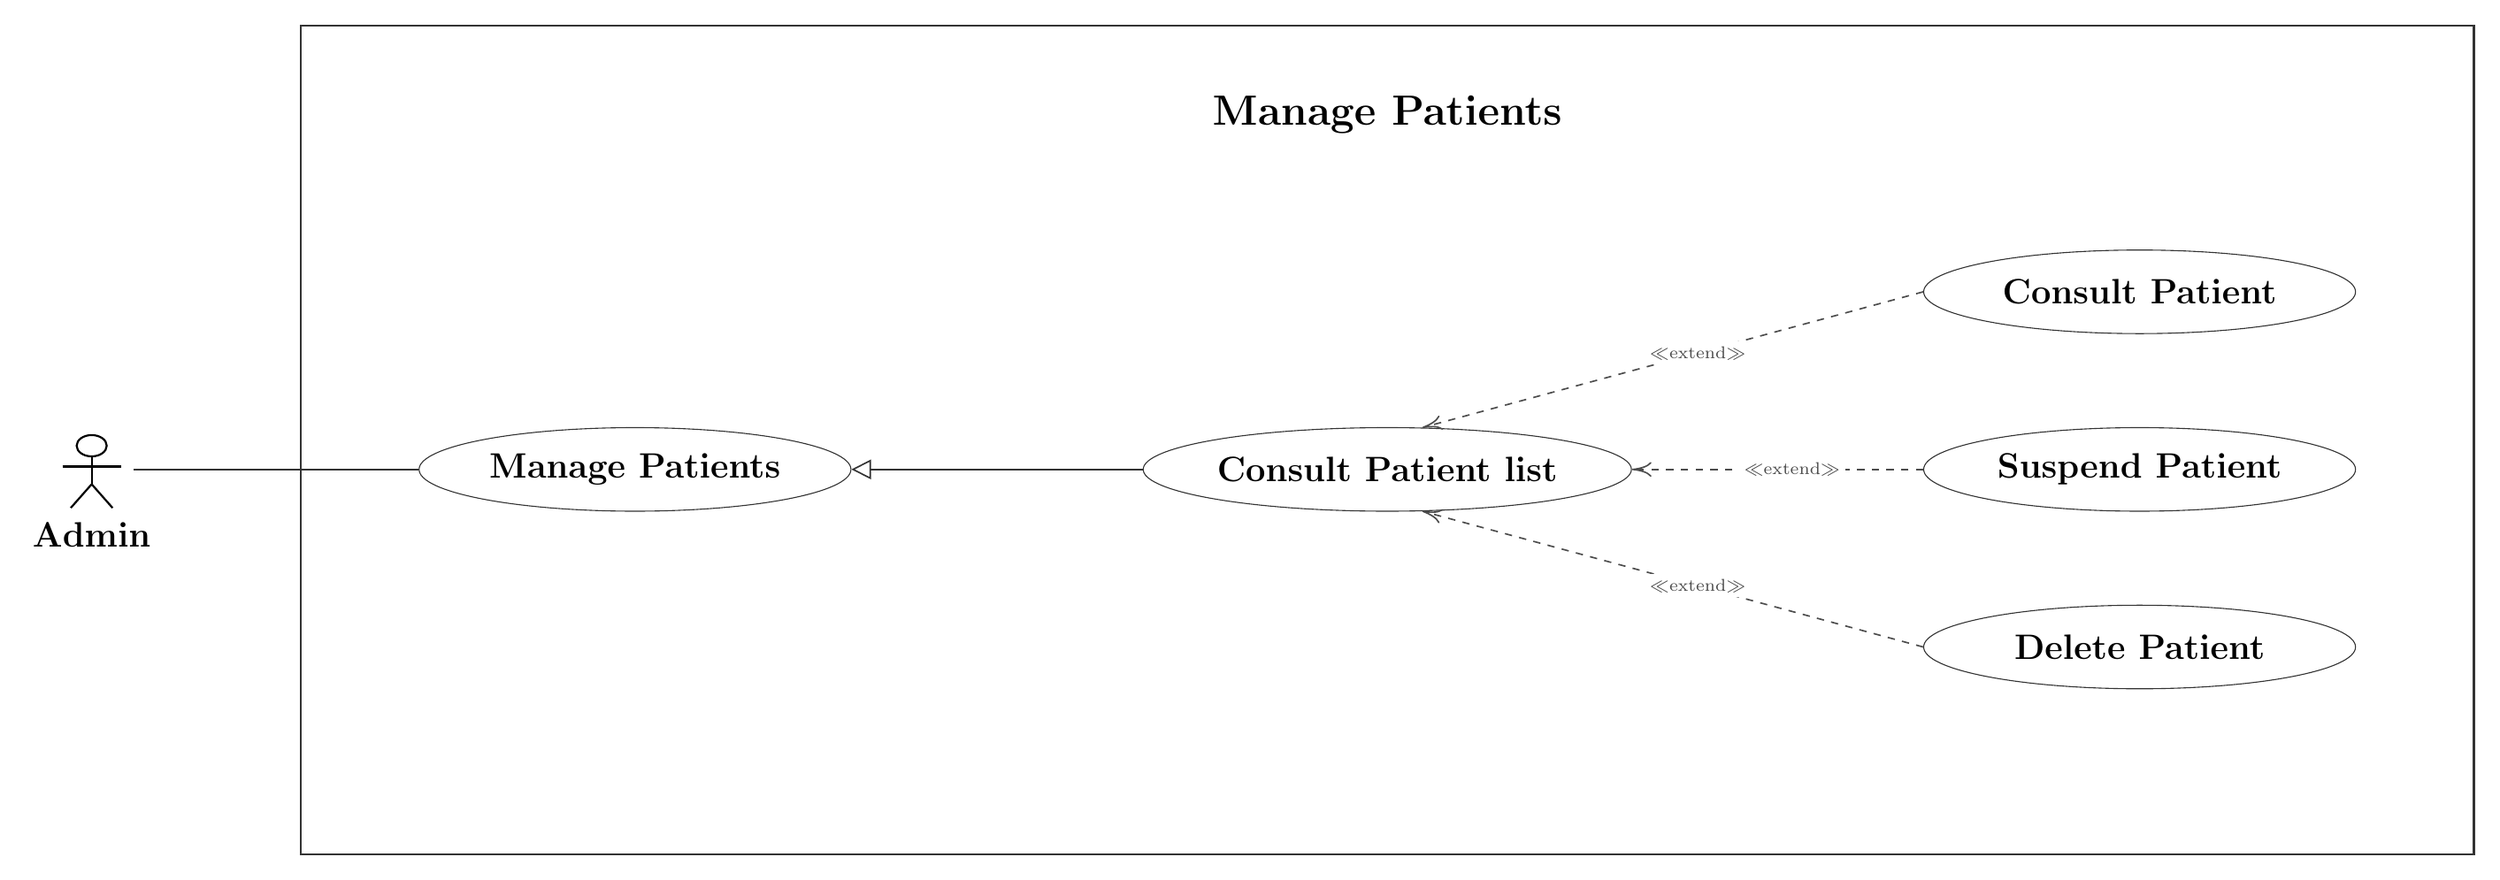
\begin{tikzpicture}[x=1.2cm,y=0.85cm]

\tikzset{
  actorlabel/.style={font=\Large\bfseries, align=center},
  usecase/.style={ellipse, draw=black!80, fill=white,
                  font=\Large\bfseries, align=center,
                  minimum width=6.2cm, minimum height=1.2cm, inner sep=1pt},
  boundary/.style={draw=black!80, line width=0.8pt},
  assoc/.style={black!80, line width=0.6pt},
  extend/.style={black!70, dashed, line width=0.6pt,
                  -{>[length=8pt, width=6pt]}},
  generalization/.style={black!80, line width=0.6pt,
                  -{Triangle[open, length=8pt, width=8pt]}}
}

\newcommand{\actor}[3]{
  \begin{scope}[shift={(#1,#2)}]
    \draw[thick] (0,0.40) circle (0.18);
    \draw[thick] (0,0.22) -- (0,-0.25);
    \draw[thick] (-0.35,0.05) -- (0.35,0.05);
    \draw[thick] (0,-0.25) -- (-0.25,-0.65);
    \draw[thick] (0,-0.25) -- (0.25,-0.65);
    \node[actorlabel, below] at (0,-0.75) {#3};
  \end{scope}
}

% Boundary and title
\draw[boundary] (-0.5, 7.5) rectangle (25.5, -6.5);
\node[font=\LARGE\bfseries] at (12.5, 6.0) {Manage Patients};

% Actor
\actor{-3.0}{0.0}{Admin}

% Root
\node[usecase] (root) at (3.5, 0.0) {Manage Patients};
\draw[assoc] (-2.5, 0.0) -- (root.west);

% Level 2
\node[usecase] (list) at (12.5, 0.0) {Consult Patient list};

% Level 3
\node[usecase] (p1) at (21.5,  3.0) {Consult Patient};
\node[usecase] (p2) at (21.5,  0.0) {Suspend Patient};
\node[usecase] (p3) at (21.5, -3.0) {Delete Patient};

% Lines
\draw[generalization] (list.west) -- (root.east);
\draw[extend] (p1.west) -- node[pos=0.45, fill=white, inner sep=2pt, font=\scriptsize] {$\ll$extend$\gg$} (list.50);
\draw[extend] (p2.west) -- node[pos=0.45, fill=white, inner sep=2pt, font=\scriptsize] {$\ll$extend$\gg$} (list.0);
\draw[extend] (p3.west) -- node[pos=0.45, fill=white, inner sep=2pt, font=\scriptsize] {$\ll$extend$\gg$} (list.-50);

\end{tikzpicture}
}
    \caption{Refined Use Case Diagram: Manage Patients}
    \label{fig:uc admin manage patients}
\end{figure}

\begin{table}[H]
\centering
\caption{Use Case Description: ``Manage Patients''}
\label{tab:uc admin manage patients}
\small
\begin{tabular}{|l|p{10cm}|}
\hline
\textbf{Use Case} & Manage Patients \\
\hline
\textbf{Primary Actor} & Administrator \\
\hline
\textbf{Preconditions} & Administrator authenticated \\
\hline
\textbf{Postconditions} & Patient accounts reviewed, suspended, or removed as needed \\
\hline
\textbf{Main Scenario} &
\begin{minipage}[t]{9.5cm}
\vspace{2pt}
1. The administrator opens the patients management page\\
2. The system displays the patients list with search and filter options (status, registration date)\\
3. The administrator selects a patient to review\\
4. The system displays the patient's full profile including medical history summary, account activity, and linked doctors\\
5. The administrator suspends the patient account due to policy violation or inactivity\\
6. The system prompts for confirmation and a reason\\
7. The administrator confirms; the system applies the suspension and logs the action\\
8. The administrator optionally deletes the patient account\\
9. The system verifies that no active medical records require retention, then proceeds with deletion or anonymization
\vspace{2pt}
\end{minipage} \\
\hline
\textbf{Alternative Flows} &
\begin{minipage}[t]{9.5cm}
\vspace{2pt}
8a. Protected record: The system denies deletion because the patient has active prescriptions or ongoing consultations. The administrator may suspend instead.\\
8b. Anonymize instead of delete: The administrator chooses to anonymize personal data while preserving medical records for regulatory compliance.\\
5a. Reactivate suspended patient: The administrator selects a suspended patient and reactivates the account; the system restores access and notifies the patient.\\
Update conflict: Another administrator modified the same record. The system refreshes and requests retry.\\
Network error: The system shows an error state and allows retry; current data is preserved.
\vspace{2pt}
\end{minipage} \\
\hline
\end{tabular}
\end{table}

\section{Class Diagram}

The class diagram represents the static structure of the core DocTIP domain, including classes, attributes, operations, and multiplicities. Figure~\ref{fig:class diagram} presents the main entities and their inheritance and association links.

\refstepcounter{figure}\label{fig:class diagram}
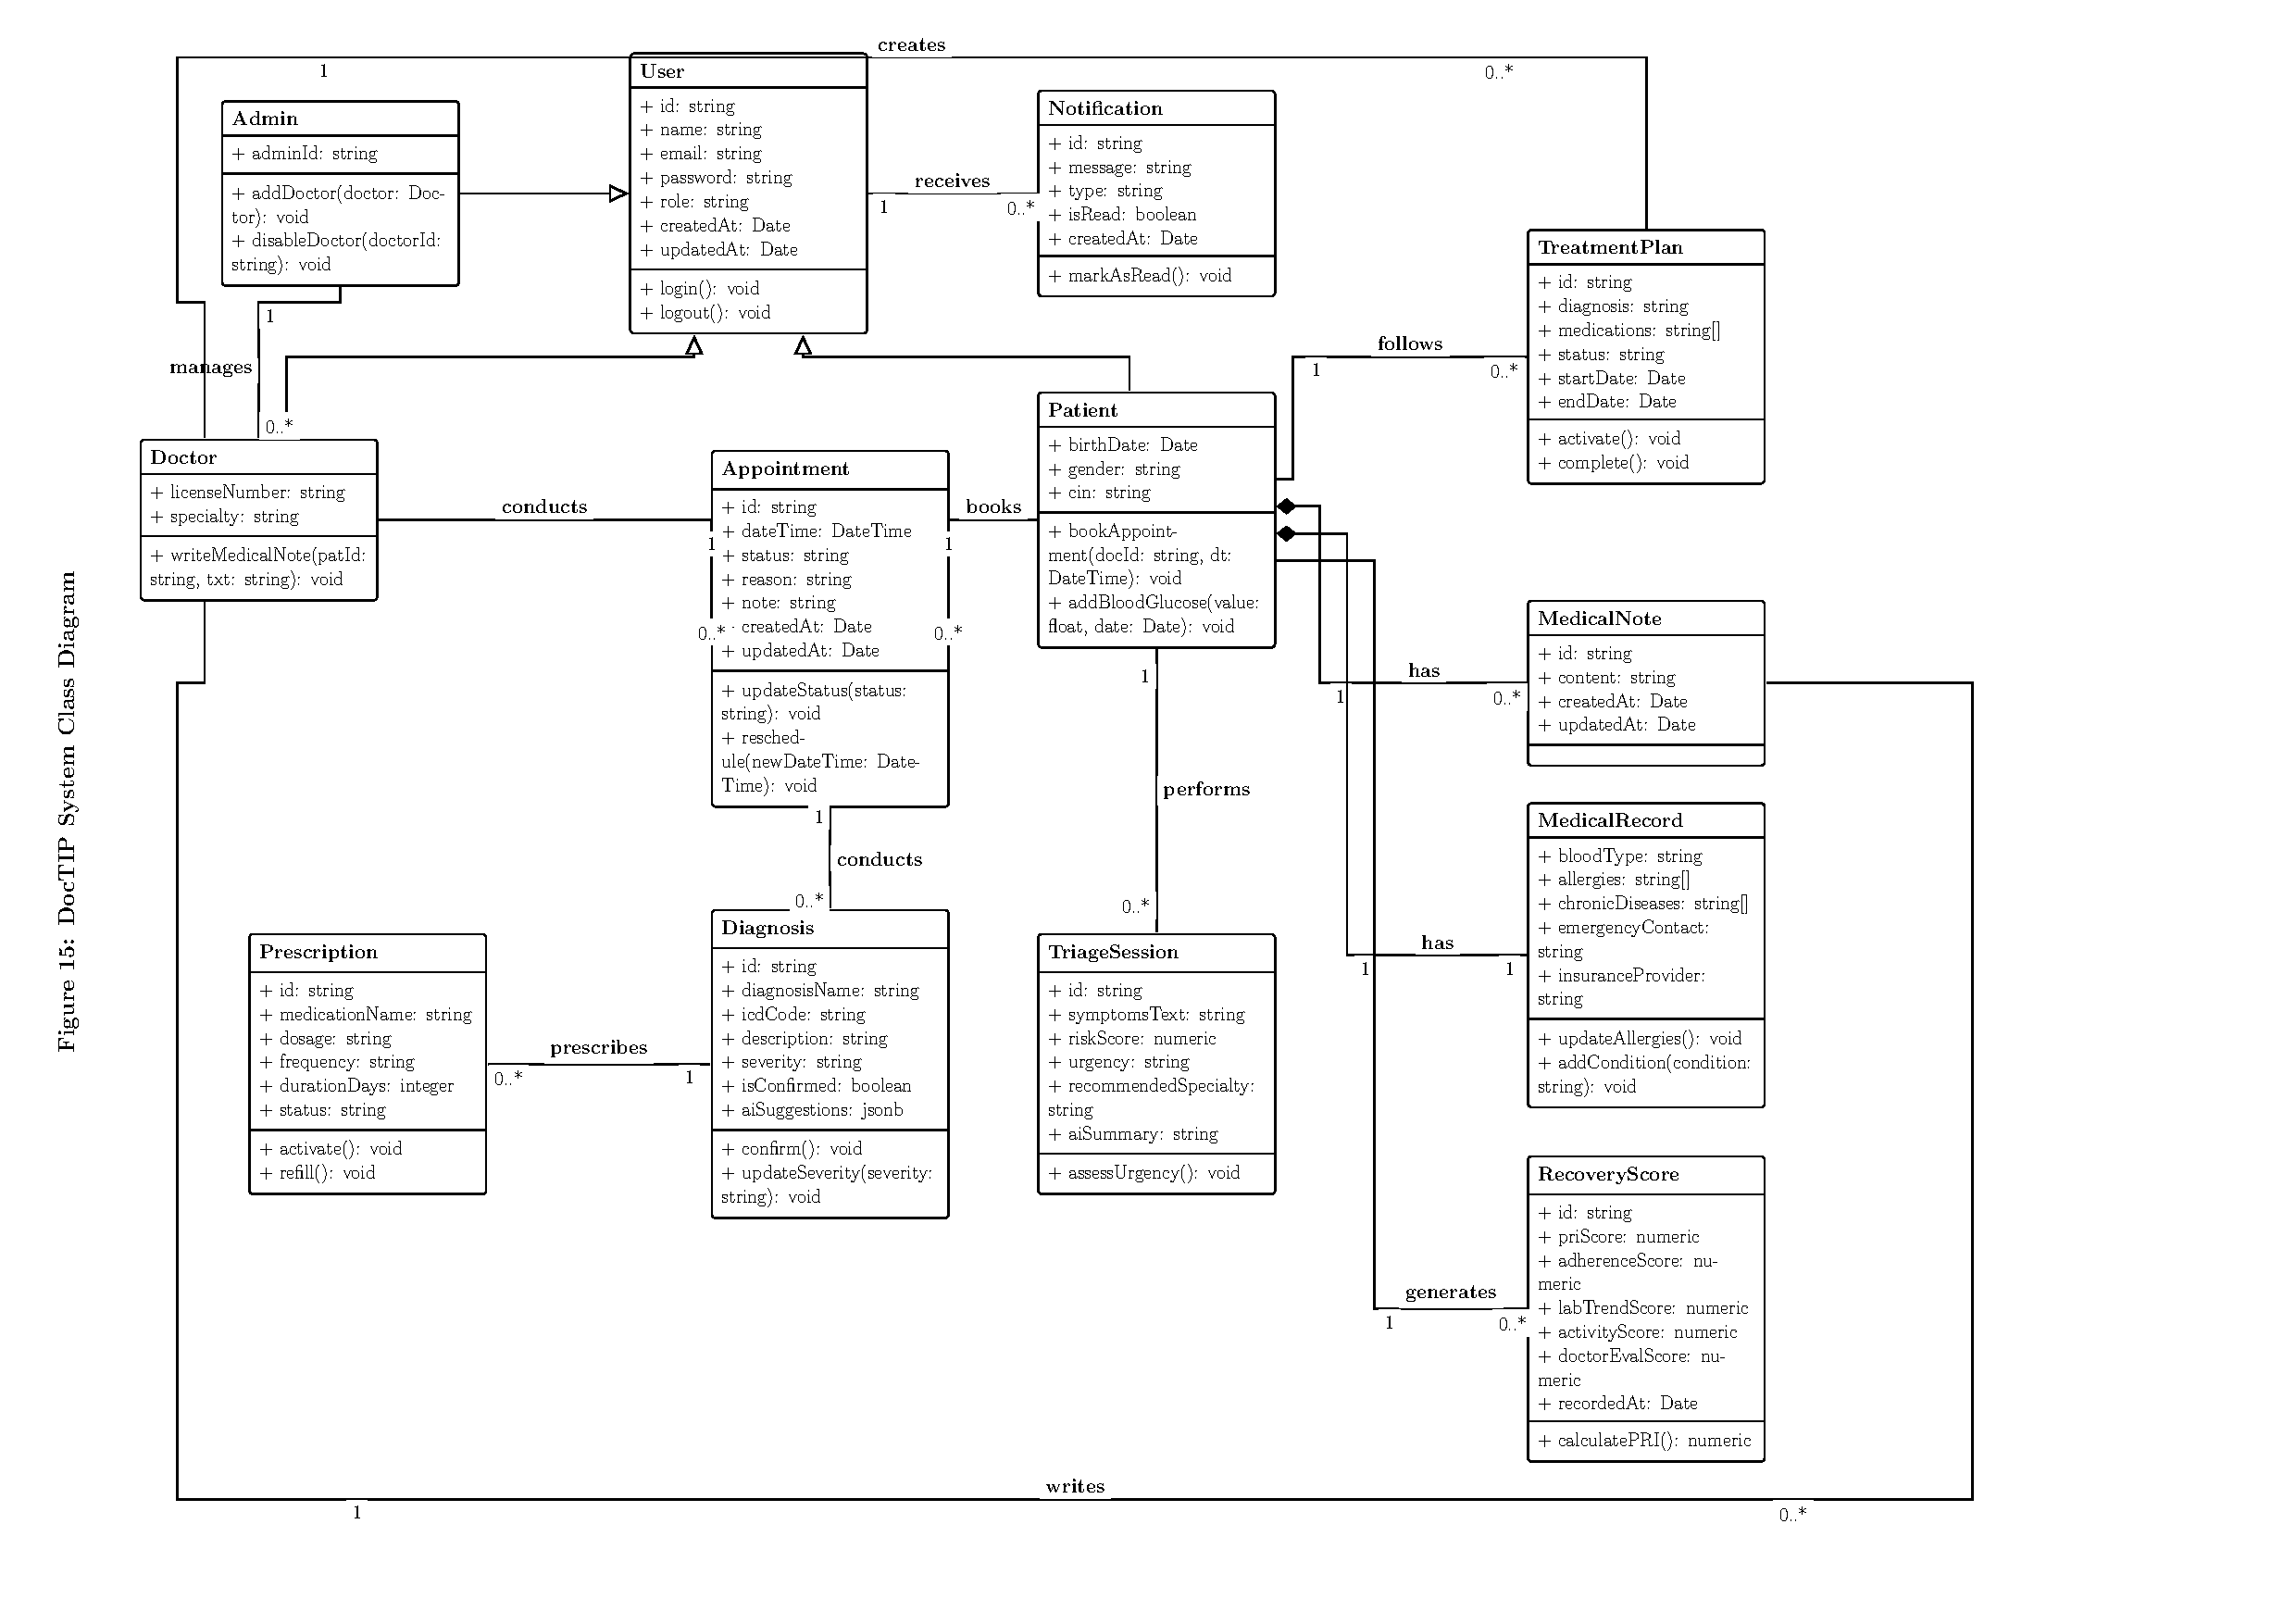
\includepdf[fitpaper=true, pages=-, pagecommand={}]{class-diagram-a3.pdf}

Below is a description of the main classes:

\begin{itemize}
    \item \textbf{Role / AppointmentStatus:} Enumerations that standardize user roles and appointment lifecycle states.
    \item \textbf{User:} Base class containing common identity and authentication attributes for all platform users.
    \item \textbf{Admin / Doctor / Patient:} Specializations of \textbf{User} that define role specific behavior.
    \item \textbf{Appointment:} Consultation scheduling entity linking doctor and patient with status tracking.
    \item \textbf{TreatmentPlan:} Structured care plan created by doctors and followed by patients.
    \item \textbf{MedicalNote:} Clinical notes written by doctors and owned by the patient lifecycle.
    \item \textbf{Notification:} User targeted communication object used for alerts and reminders.
\end{itemize}

% TikZ source: figures/tikz/class diagram.tex

\section{Sequence Diagrams}

The sequence diagram describes how system elements interact with each other by specifying the different messages exchanged in chronological order. We detail below the most representative scenarios.

\subsection{Authentication Sequence Diagram}

To authenticate, the user enters their email and password. The system verifies the credentials via Supabase Auth. If the account exists and the information is correct, a JWT token is assigned and the user is redirected to their portal according to their role. Figure~\ref{fig:seq auth} illustrates this process.

\begin{figure}[H]
    \centering
    \resizebox{0.92\textwidth}{!}{% DoctIP Sequence Diagram: Authentication (structured with loop/alt)
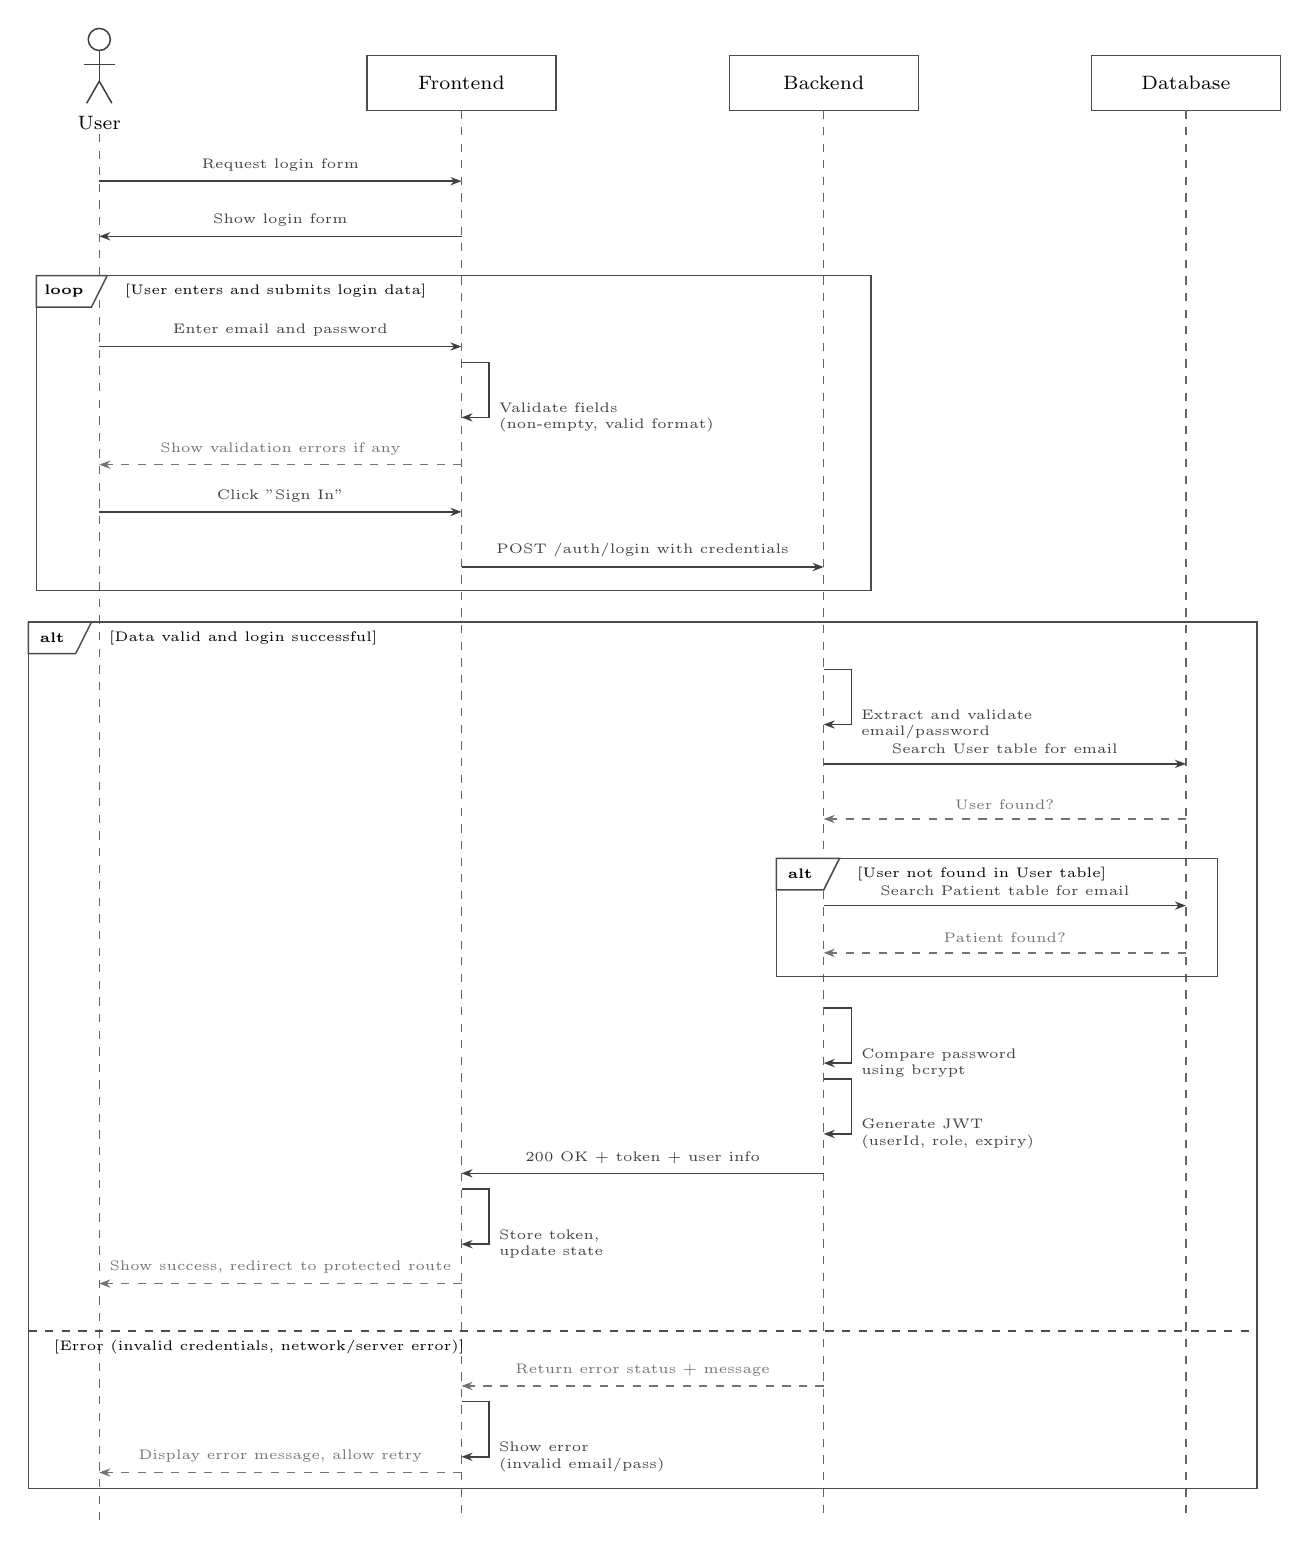
\begin{tikzpicture}[x=1cm,y=1cm]
  \tikzset{
    life/.style={black!60, dashed, line width=0.5pt},
    part/.style={draw=black!70, fill=white, minimum width=2.4cm, minimum height=0.7cm, align=center, font=\scriptsize},
    msg/.style={-{Stealth[length=4pt]}, black!75, line width=0.55pt, font=\tiny},
    ret/.style={-{Stealth[length=4pt]}, black!55, dashed, line width=0.5pt, font=\tiny},
    frame/.style={draw=black!70, line width=0.55pt}
  }

  % X positions spanning wide enough to prevent overlap
  \def\xU{0}
  \def\xA{4.6}
  \def\xS{9.2}
  \def\xD{13.8}

  % User actor (stick figure)
  \begin{scope}[shift={(\xU,0.25)}]
    \draw[black!75, line width=0.55pt] (0,0.35) circle (0.14cm);
    \draw[black!75, line width=0.55pt] (0,0.21)--(0,-0.18);
    \draw[black!75, line width=0.55pt] (-0.20,0.03)--(0.20,0.03);
    \draw[black!75, line width=0.55pt] (0,-0.18)--(-0.16,-0.46);
    \draw[black!75, line width=0.55pt] (0,-0.18)--(0.16,-0.46);
    \node[font=\scriptsize, below] at (0,-0.50) {User};
  \end{scope}

  % Other participants
  \node[part] (app) at (\xA,0.05) {Frontend};
  \node[part] (auth) at (\xS,0.05) {Backend};
  \node[part] (db) at (\xD,0.05) {Database};

  % Lifelines
  \draw[life] (\xU,-0.6) -- (\xU,-18.2);
  \draw[life] (\xA,-0.3) -- (\xA,-18.2);
  \draw[life] (\xS,-0.3) -- (\xS,-18.2);
  \draw[life] (\xD,-0.3) -- (\xD,-18.2);

  % Messages before loop
  \draw[msg] (\xU,-1.2) -- node[above] {Request login form} (\xA,-1.2);
  \draw[msg] (\xA,-1.9) -- node[above] {Show login form} (\xU,-1.9);

  % ================= LOOP FRAME =================
  \def\lyT{-2.4}\def\lyB{-6.4}\def\lxL{-0.8}\def\lxR{\xS+0.6}
  \draw[frame] (\lxL,\lyT) rectangle (\lxR,\lyB);
  \draw[frame, fill=white] (\lxL,\lyT) -- ++(0,-0.4) -- ++(0.7,0) -- ++(0.2,0.4) -- cycle;
  \node[font=\tiny] at (\lxL+0.35,\lyT-0.2) {\textbf{loop}};
  \node[font=\tiny, anchor=west] at (\lxL+1.0,\lyT-0.2) {[User enters and submits login data]};

  \draw[msg] (\xU,-3.3) -- node[above] {Enter email and password} (\xA,-3.3);
  \draw[msg] (\xA,-3.5) -- +(0.35,0) |- node[right, align=left] {Validate fields\\(non-empty, valid format)} (\xA,-4.2);
  \draw[ret] (\xA,-4.8) -- node[above] {Show validation errors if any} (\xU,-4.8);
  \draw[msg] (\xU,-5.4) -- node[above] {Click "Sign In"} (\xA,-5.4);
  \draw[msg] (\xA,-6.1) -- node[above] {POST /auth/login with credentials} (\xS,-6.1);

  % ================= MAIN ALT FRAME =================
  \def\ayT{-6.8}\def\ayB{-17.8}\def\axL{-0.9}\def\axR{\xD+0.9}
  \draw[frame] (\axL,\ayT) rectangle (\axR,\ayB);
  \draw[frame, fill=white] (\axL,\ayT) -- ++(0,-0.4) -- ++(0.6,0) -- ++(0.2,0.4) -- cycle;
  \node[font=\tiny] at (\axL+0.3,\ayT-0.2) {\textbf{alt}};
  \node[font=\tiny, anchor=west] at (\axL+0.9,\ayT-0.2) {[Data valid and login successful]};

  \draw[msg] (\xS,-7.4) -- +(0.35,0) |- node[right, align=left] {Extract and validate\\email/password} (\xS,-8.1);
  \draw[msg] (\xS,-8.6) -- node[above] {Search User table for email} (\xD,-8.6);
  \draw[ret] (\xD,-9.3) -- node[above] {User found?} (\xS,-9.3);

  % ================= NESTED ALT FRAME =================
  \def\nyT{-9.8}\def\nyB{-11.3}\def\nxL{\xS-0.6}\def\nxR{\xD+0.4}
  \draw[frame] (\nxL,\nyT) rectangle (\nxR,\nyB);
  \draw[frame, fill=white] (\nxL,\nyT) -- ++(0,-0.4) -- ++(0.6,0) -- ++(0.2,0.4) -- cycle;
  \node[font=\tiny] at (\nxL+0.3,\nyT-0.2) {\textbf{alt}};
  \node[font=\tiny, anchor=west] at (\nxL+0.9,\nyT-0.2) {[User not found in User table]};

  \draw[msg] (\xS,-10.4) -- node[above] {Search Patient table for email} (\xD,-10.4);
  \draw[ret] (\xD,-11.0) -- node[above] {Patient found?} (\xS,-11.0);

  \draw[msg] (\xS,-11.7) -- +(0.35,0) |- node[right, align=left] {Compare password\\using bcrypt} (\xS,-12.4);
  \draw[msg] (\xS,-12.6) -- +(0.35,0) |- node[right, align=left] {Generate JWT\\(userId, role, expiry)} (\xS,-13.3);

  \draw[msg] (\xS,-13.8) -- node[above] {200 OK + token + user info} (\xA,-13.8);
  \draw[msg] (\xA,-14.0) -- +(0.35,0) |- node[right, align=left] {Store token,\\update state} (\xA,-14.7);
  \draw[ret] (\xA,-15.2) -- node[above] {Show success, redirect to protected route} (\xU,-15.2);

  % ================= ELSE SEPARATOR =================
  \def\ey{-15.8}
  \draw[frame, dashed] (\axL,\ey) -- (\axR,\ey);
  \node[font=\tiny, anchor=west] at (\axL+0.2,\ey-0.2) {[Error (invalid credentials, network/server error)]};

  \draw[ret] (\xS,-16.5) -- node[above] {Return error status + message} (\xA,-16.5);
  \draw[msg] (\xA,-16.7) -- +(0.35,0) |- node[right, align=left] {Show error\\(invalid email/pass)} (\xA,-17.4);
  \draw[ret] (\xA,-17.6) -- node[above] {Display error message, allow retry} (\xU,-17.6);

\end{tikzpicture}

}
    \caption{Sequence Diagram: Authentication}
    \label{fig:seq auth}
\end{figure}

% PlantUML source: figures/plantuml/seq auth.puml

\subsection{AI Symptom Triage Sequence Diagram}

The AI triage process allows the patient to describe their symptoms and receive an urgency assessment powered by GPT 4. Figure~\ref{fig:seq triage} illustrates this process.

\begin{figure}[H]
    \centering
    \resizebox{0.92\textwidth}{!}{% DoctIP Sequence Diagram: AI Symptom Triage
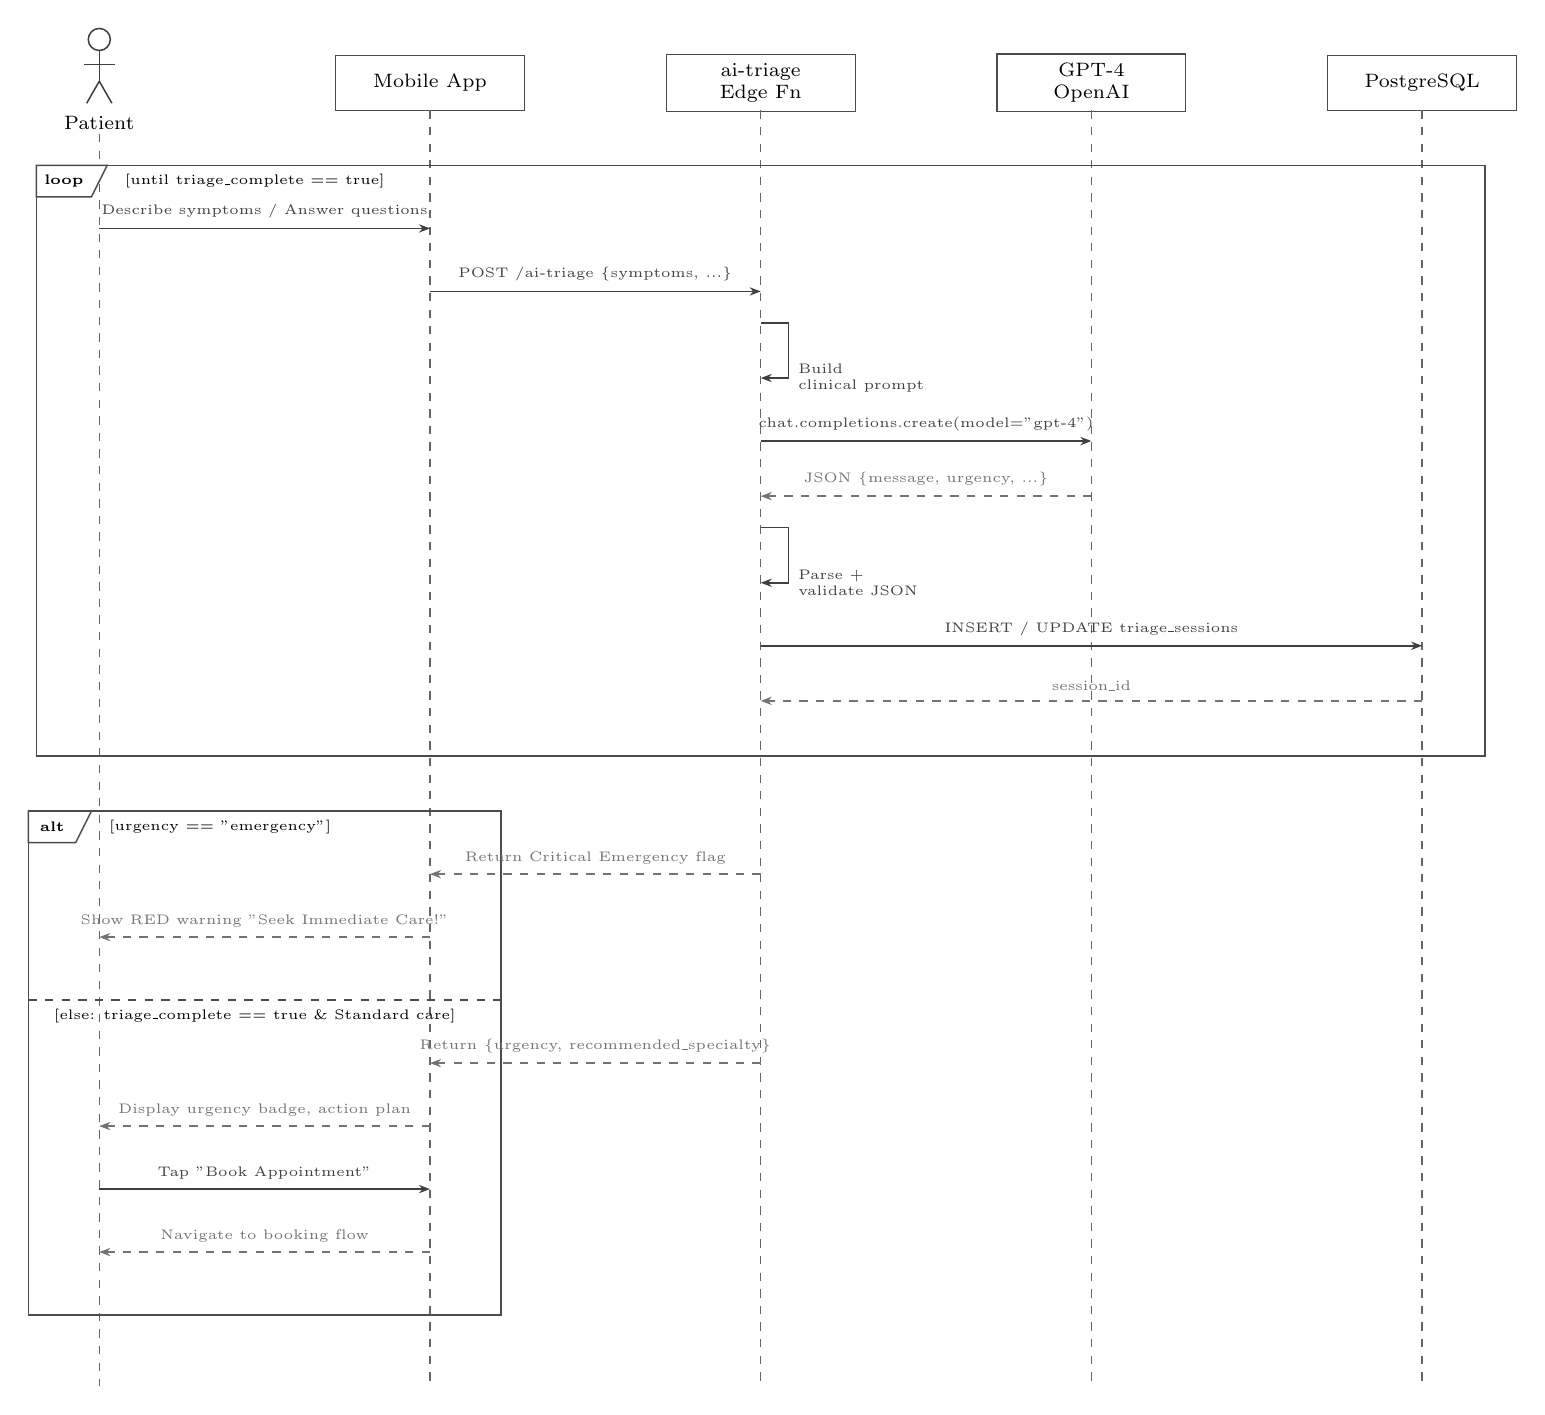
\begin{tikzpicture}[x=1cm,y=1cm]
  \tikzset{
    life/.style={black!60, dashed, line width=0.5pt},
    part/.style={draw=black!70, fill=white, minimum width=2.4cm, minimum height=0.7cm, align=center, font=\scriptsize},
    msg/.style={-{Stealth[length=4pt]}, black!75, line width=0.55pt, font=\tiny},
    ret/.style={-{Stealth[length=4pt]}, black!55, dashed, line width=0.5pt, font=\tiny},
    frame/.style={draw=black!70, line width=0.55pt},
    note/.style={draw=black!70, fill=black!5, rounded corners=2pt, font=\tiny, align=left, inner sep=3pt}
  }

  % X positions spanning wide enough to prevent overlap
  \def\xU{0}
  \def\xA{4.2}
  \def\xE{8.4}
  \def\xG{12.6}
  \def\xD{16.8}

  % Patient actor (stick figure)
  \begin{scope}[shift={(\xU,0.25)}]
    \draw[black!75, line width=0.55pt] (0,0.35) circle (0.14cm);
    \draw[black!75, line width=0.55pt] (0,0.21)--(0,-0.18);
    \draw[black!75, line width=0.55pt] (-0.20,0.03)--(0.20,0.03);
    \draw[black!75, line width=0.55pt] (0,-0.18)--(-0.16,-0.46);
    \draw[black!75, line width=0.55pt] (0,-0.18)--(0.16,-0.46);
    \node[font=\scriptsize, below] at (0,-0.50) {Patient};
  \end{scope}

  % Other participants
  \node[part] (app) at (\xA,0.05) {Mobile App};
  \node[part] (fn) at (\xE,0.05) {ai-triage\\Edge Fn};
  \node[part] (gpt) at (\xG,0.05) {GPT-4\\OpenAI};
  \node[part] (db) at (\xD,0.05) {PostgreSQL};

  % Lifelines
  \draw[life] (\xU,-0.6) -- (\xU,-16.5);
  \draw[life] (\xA,-0.3) -- (\xA,-16.5);
  \draw[life] (\xE,-0.3) -- (\xE,-16.5);
  \draw[life] (\xG,-0.3) -- (\xG,-16.5);
  \draw[life] (\xD,-0.3) -- (\xD,-16.5);

  % ================= LOOP FRAME =================
  \def\lyT{-1.0}\def\lyB{-8.5}\def\lxL{-0.8}\def\lxR{\xD+0.8}
  \draw[frame] (\lxL,\lyT) rectangle (\lxR,\lyB);
  \draw[frame, fill=white] (\lxL,\lyT) -- ++(0,-0.4) -- ++(0.7,0) -- ++(0.2,0.4) -- cycle;
  \node[font=\tiny] at (\lxL+0.35,\lyT-0.2) {\textbf{loop}};
  \node[font=\tiny, anchor=west] at (\lxL+1.0,\lyT-0.2) {[until triage\_complete == true]};

  % Messages inside loop
  \draw[msg] (\xU,-1.8) -- node[above] {Describe symptoms / Answer questions} (\xA,-1.8);
  \draw[msg] (\xA,-2.6) -- node[above] {POST /ai-triage \{symptoms, ...\}} (\xE,-2.6);
  
  \draw[msg] (\xE,-3.0) -- +(0.35,0) |- node[right, align=left] {Build\\clinical prompt} (\xE,-3.7);

  \draw[msg] (\xE,-4.5) -- node[above] {chat.completions.create(model="gpt-4")} (\xG,-4.5);
  \draw[ret] (\xG,-5.2) -- node[above] {JSON \{message, urgency, ...\}} (\xE,-5.2);

  \draw[msg] (\xE,-5.6) -- +(0.35,0) |- node[right, align=left] {Parse +\\validate JSON} (\xE,-6.3);

  \draw[msg] (\xE,-7.1) -- node[above] {INSERT / UPDATE triage\_sessions} (\xD,-7.1);
  \draw[ret] (\xD,-7.8) -- node[above] {session\_id} (\xE,-7.8);

  % ================= ALT FRAME =================
  \def\ayT{-9.2}\def\ayB{-15.6}\def\axL{-0.9}\def\axR{\xA+0.9}
  \draw[frame] (\axL,\ayT) rectangle (\axR,\ayB);
  \draw[frame, fill=white] (\axL,\ayT) -- ++(0,-0.4) -- ++(0.6,0) -- ++(0.2,0.4) -- cycle;
  \node[font=\tiny] at (\axL+0.3,\ayT-0.2) {\textbf{alt}};
  \node[font=\tiny, anchor=west] at (\axL+0.9,\ayT-0.2) {[urgency == "emergency"]};
  
  % Branch 1: Critical Emergency
  \draw[ret] (\xE,-10.0) -- node[above] {Return Critical Emergency flag} (\xA,-10.0);
  \draw[ret] (\xA,-10.8) -- node[above] {Show RED warning "Seek Immediate Care!"} (\xU,-10.8);

  % ================= ELSE SEPARATOR =================
  \def\ey{-11.6}
  \draw[frame, dashed] (\axL,\ey) -- (\axR,\ey);
  \node[font=\tiny, anchor=west] at (\axL+0.2,\ey-0.2) {[else: triage\_complete == true \& Standard care]};
  
  \draw[ret] (\xE,-12.4) -- node[above] {Return \{urgency, recommended\_specialty\}} (\xA,-12.4);
  \draw[ret] (\xA,-13.2) -- node[above] {Display urgency badge, action plan} (\xU,-13.2);
  
  \draw[msg] (\xU,-14.0) -- node[above] {Tap "Book Appointment"} (\xA,-14.0);
  \draw[ret] (\xA,-14.8) -- node[above] {Navigate to booking flow} (\xU,-14.8);

\end{tikzpicture}

}
    \caption{Sequence Diagram: AI Symptom Triage}
    \label{fig:seq triage}
\end{figure}

% PlantUML source: figures/plantuml/seq triage.puml

\subsection{AI Clinical Diagnostic Assistance Sequence Diagram}

This diagram illustrates the interaction between the doctor, the clinical support Edge Function, and OpenAI GPT 4 for diagnostic assistance. Figure~\ref{fig:seq clinical ai} presents this flow.

\begin{figure}[H]
    \centering
    \resizebox{0.92\textwidth}{!}{% DoctIP Sequence Diagram: AI Clinical Diagnostic Assistance
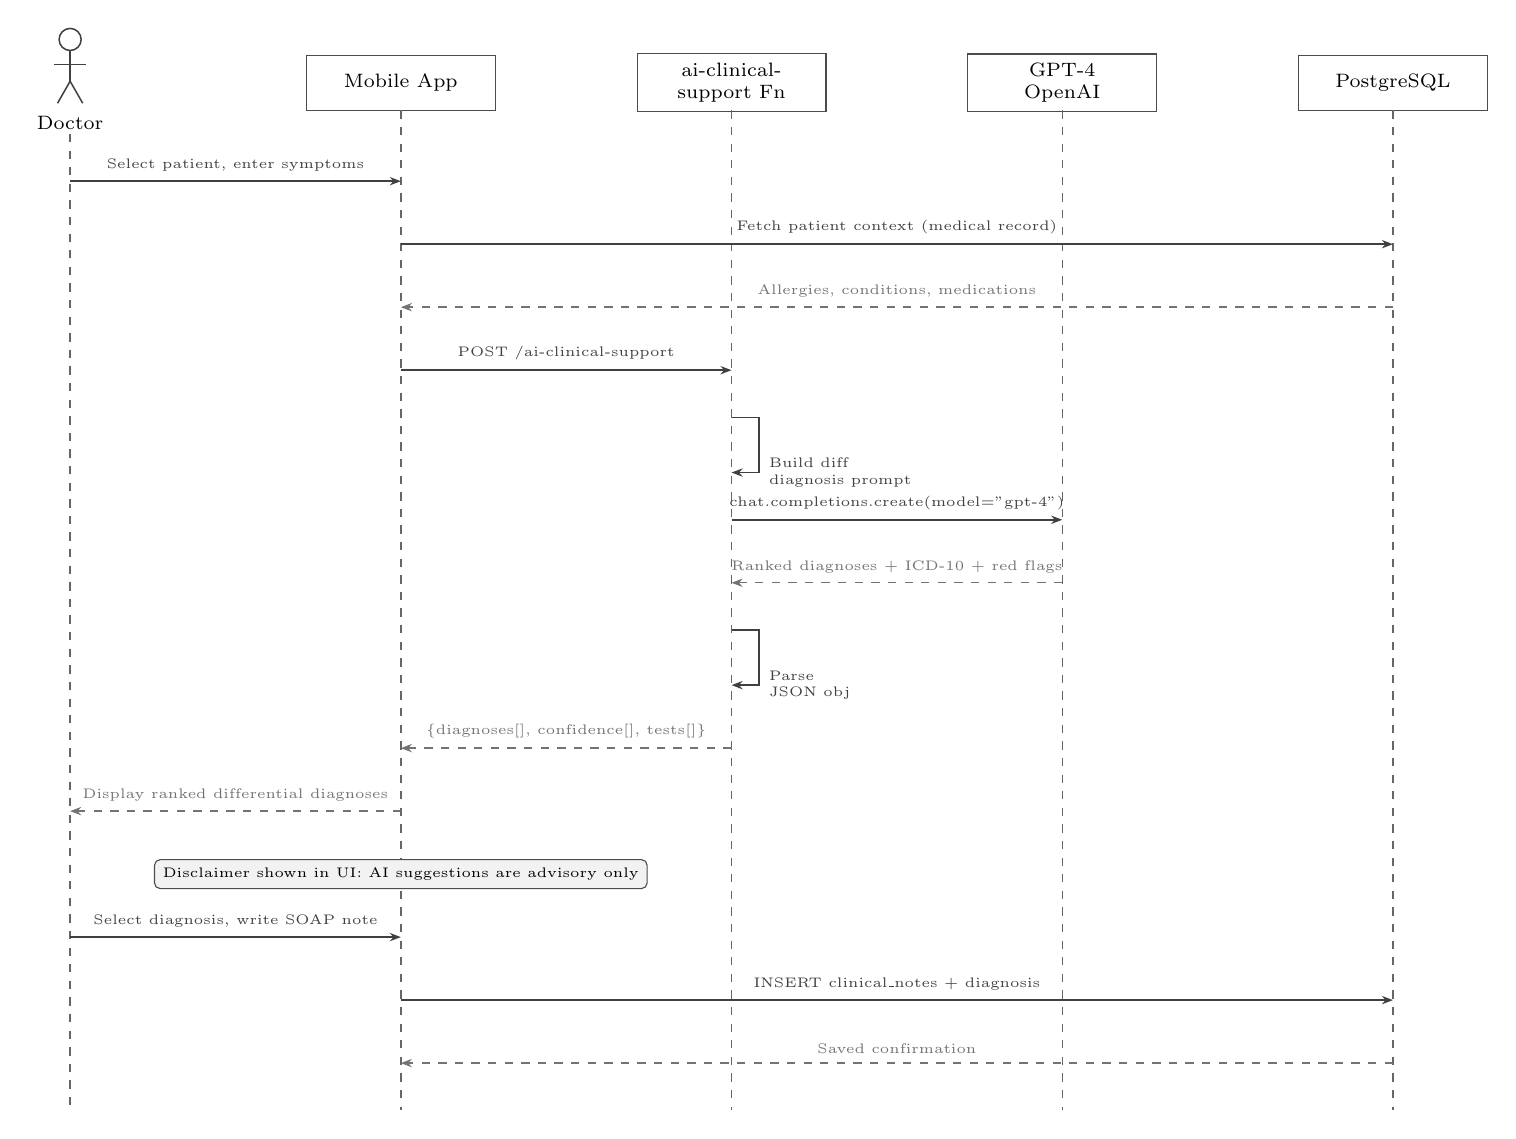
\begin{tikzpicture}[x=1cm,y=1cm]
  \tikzset{
    life/.style={black!60, dashed, line width=0.5pt},
    part/.style={draw=black!70, fill=white, minimum width=2.4cm, minimum height=0.7cm, align=center, font=\scriptsize},
    msg/.style={-{Stealth[length=4pt]}, black!75, line width=0.55pt, font=\tiny},
    ret/.style={-{Stealth[length=4pt]}, black!55, dashed, line width=0.5pt, font=\tiny},
    frame/.style={draw=black!70, line width=0.55pt},
    note/.style={draw=black!70, fill=black!5, rounded corners=2pt, font=\tiny, align=left, inner sep=3pt}
  }

  % X positions (widened to 4.2 to prevent overlap)
  \def\xD{0}
  \def\xA{4.2}
  \def\xE{8.4}
  \def\xG{12.6}
  \def\xDB{16.8}

  % Doctor actor (stick figure)
  \begin{scope}[shift={(\xD,0.25)}]
    \draw[black!75, line width=0.55pt] (0,0.35) circle (0.14cm);
    \draw[black!75, line width=0.55pt] (0,0.21)--(0,-0.18);
    \draw[black!75, line width=0.55pt] (-0.20,0.03)--(0.20,0.03);
    \draw[black!75, line width=0.55pt] (0,-0.18)--(-0.16,-0.46);
    \draw[black!75, line width=0.55pt] (0,-0.18)--(0.16,-0.46);
    \node[font=\scriptsize, below] at (0,-0.50) {Doctor};
  \end{scope}

  % Other participants
  \node[part] (app) at (\xA,0.05) {Mobile App};
  \node[part] (fn) at (\xE,0.05) {ai-clinical-\\support Fn};
  \node[part] (gpt) at (\xG,0.05) {GPT-4\\OpenAI};
  \node[part] (db) at (\xDB,0.05) {PostgreSQL};

  % Lifelines
  \draw[life] (\xD,-0.6) -- (\xD,-13.0);
  \draw[life] (\xA,-0.3) -- (\xA,-13.0);
  \draw[life] (\xE,-0.3) -- (\xE,-13.0);
  \draw[life] (\xG,-0.3) -- (\xG,-13.0);
  \draw[life] (\xDB,-0.3) -- (\xDB,-13.0);

  % Messages
  \draw[msg] (\xD,-1.2) -- node[above] {Select patient, enter symptoms} (\xA,-1.2);
  \draw[msg] (\xA,-2.0) -- node[above] {Fetch patient context (medical record)} (\xDB,-2.0);
  \draw[ret] (\xDB,-2.8) -- node[above] {Allergies, conditions, medications} (\xA,-2.8);
  
  \draw[msg] (\xA,-3.6) -- node[above] {POST /ai-clinical-support} (\xE,-3.6);
  
  \draw[msg] (\xE,-4.2) -- +(0.35,0) |- node[right, align=left] {Build diff\\diagnosis prompt} (\xE,-4.9);
  
  \draw[msg] (\xE,-5.5) -- node[above] {chat.completions.create(model="gpt-4")} (\xG,-5.5);
  \draw[ret] (\xG,-6.3) -- node[above] {Ranked diagnoses + ICD-10 + red flags} (\xE,-6.3);
  
  \draw[msg] (\xE,-6.9) -- +(0.35,0) |- node[right, align=left] {Parse\\JSON obj} (\xE,-7.6);
  
  \draw[ret] (\xE,-8.4) -- node[above] {\{diagnoses[], confidence[], tests[]\}} (\xA,-8.4);
  \draw[ret] (\xA,-9.2) -- node[above] {Display ranked differential diagnoses} (\xD,-9.2);

  \node[note] at (\xA,-10.0) {Disclaimer shown in UI: AI suggestions are advisory only};
  
  \draw[msg] (\xD,-10.8) -- node[above] {Select diagnosis, write SOAP note} (\xA,-10.8);
  \draw[msg] (\xA,-11.6) -- node[above] {INSERT clinical\_notes + diagnosis} (\xDB,-11.6);
  \draw[ret] (\xDB,-12.4) -- node[above] {Saved confirmation} (\xA,-12.4);

\end{tikzpicture}

}
    \caption{Sequence Diagram: AI Clinical Diagnostic Assistance}
    \label{fig:seq clinical ai}
\end{figure}

% PlantUML source: figures/plantuml/seq clinical ai.puml

\subsection{Login Anomaly Detection Sequence Diagram}

The Zero Trust system verifies every login attempt. Figure~\ref{fig:seq anomaly} illustrates this process.

\begin{figure}[H]
    \centering
    \resizebox{\textwidth}{!}{% DoctIP Sequence Diagram: Login Anomaly Detection (Zero-Trust)
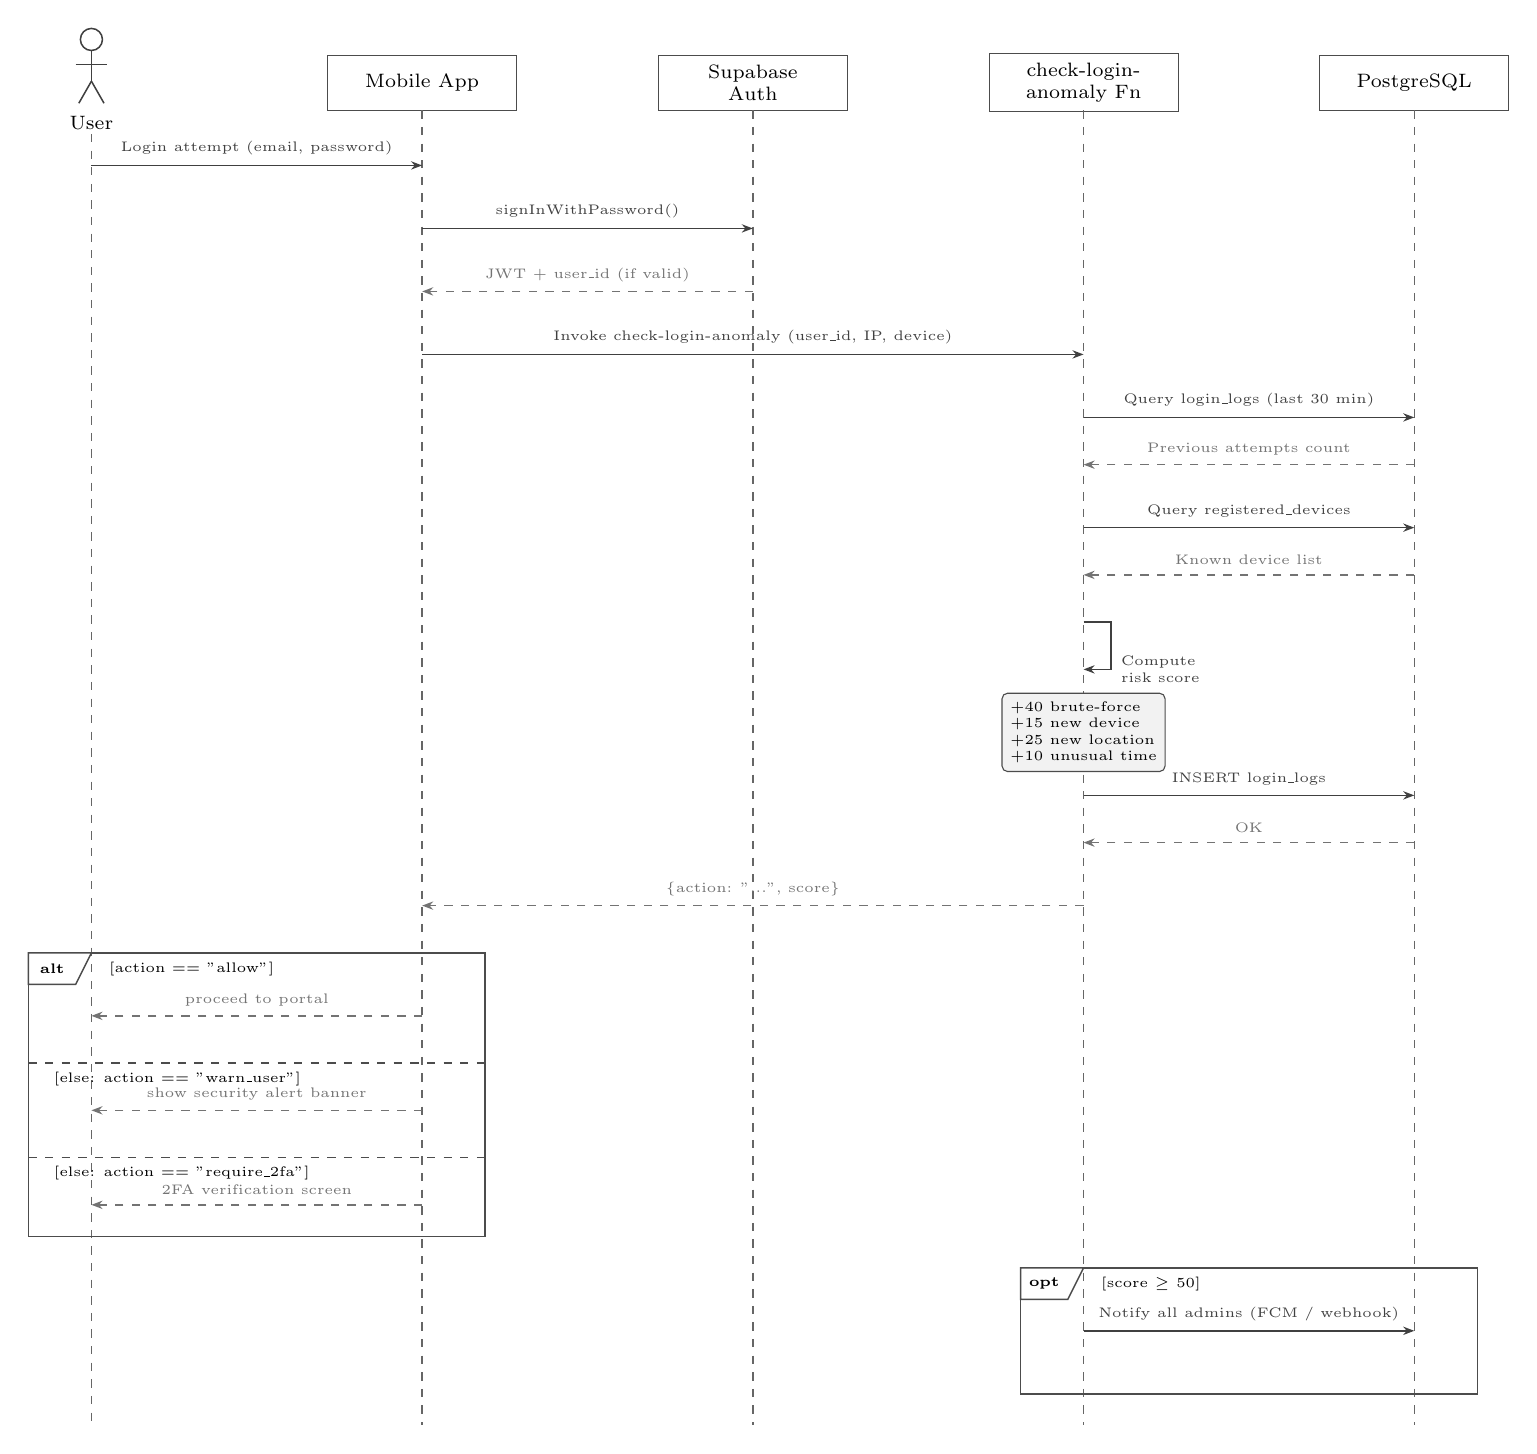
\begin{tikzpicture}[x=1cm,y=1cm]
  \tikzset{
    life/.style={black!60, dashed, line width=0.5pt},
    part/.style={draw=black!70, fill=white, minimum width=2.4cm, minimum height=0.7cm, align=center, font=\scriptsize},
    msg/.style={-{Stealth[length=4pt]}, black!75, line width=0.55pt, font=\tiny},
    ret/.style={-{Stealth[length=4pt]}, black!55, dashed, line width=0.5pt, font=\tiny},
    frame/.style={draw=black!70, line width=0.55pt},
    note/.style={draw=black!70, fill=black!5, rounded corners=2pt, font=\tiny, align=left, inner sep=3pt}
  }

  % X positions (widened to 4.2 spacing)
  \def\xU{0}
  \def\xA{4.2}
  \def\xS{8.4}
  \def\xAn{12.6}
  \def\xD{16.8}

  % User actor (stick figure)
  \begin{scope}[shift={(\xU,0.25)}]
    \draw[black!75, line width=0.55pt] (0,0.35) circle (0.14cm);
    \draw[black!75, line width=0.55pt] (0,0.21)--(0,-0.18);
    \draw[black!75, line width=0.55pt] (-0.20,0.03)--(0.20,0.03);
    \draw[black!75, line width=0.55pt] (0,-0.18)--(-0.16,-0.46);
    \draw[black!75, line width=0.55pt] (0,-0.18)--(0.16,-0.46);
    \node[font=\scriptsize, below] at (0,-0.50) {User};
  \end{scope}

  % Other participants
  \node[part] (app) at (\xA,0.05) {Mobile App};
  \node[part] (auth) at (\xS,0.05) {Supabase\\Auth};
  \node[part] (fn) at (\xAn,0.05) {check-login-\\anomaly Fn};
  \node[part] (db) at (\xD,0.05) {PostgreSQL};

  % Lifelines
  \draw[life] (\xU,-0.6) -- (\xU,-17.0);
  \draw[life] (\xA,-0.3) -- (\xA,-17.0);
  \draw[life] (\xS,-0.3) -- (\xS,-17.0);
  \draw[life] (\xAn,-0.3) -- (\xAn,-17.0);
  \draw[life] (\xD,-0.3) -- (\xD,-17.0);

  % Messages
  \draw[msg] (\xU,-1.0) -- node[above] {Login attempt (email, password)} (\xA,-1.0);
  \draw[msg] (\xA,-1.8) -- node[above] {signInWithPassword()} (\xS,-1.8);
  \draw[ret] (\xS,-2.6) -- node[above] {JWT + user\_id (if valid)} (\xA,-2.6);
  
  \draw[msg] (\xA,-3.4) -- node[above] {Invoke check-login-anomaly (user\_id, IP, device)} (\xAn,-3.4);
  
  \draw[msg] (\xAn,-4.2) -- node[above] {Query login\_logs (last 30 min)} (\xD,-4.2);
  \draw[ret] (\xD,-4.8) -- node[above] {Previous attempts count} (\xAn,-4.8);
  
  \draw[msg] (\xAn,-5.6) -- node[above] {Query registered\_devices} (\xD,-5.6);
  \draw[ret] (\xD,-6.2) -- node[above] {Known device list} (\xAn,-6.2);
  
  \draw[msg] (\xAn,-6.8) -- +(0.35,0) |- node[right, align=left] {Compute\\risk score} (\xAn,-7.4);
  
  \node[note] at (\xAn,-8.2) {+40 brute-force\\+15 new device\\+25 new location\\+10 unusual time};
  
  \draw[msg] (\xAn,-9.0) -- node[above] {INSERT login\_logs} (\xD,-9.0);
  \draw[ret] (\xD,-9.6) -- node[above] {OK} (\xAn,-9.6);
  
  \draw[ret] (\xAn,-10.4) -- node[above] {\{action: "...", score\}} (\xA,-10.4);

  % ================= ACTION ALT FRAME =================
  \def\ayT{-11.0}\def\ayB{-14.6}\def\axL{-0.8}\def\axR{\xA+0.8}
  \draw[frame] (\axL,\ayT) rectangle (\axR,\ayB);
  \draw[frame, fill=white] (\axL,\ayT) -- ++(0,-0.4) -- ++(0.6,0) -- ++(0.2,0.4) -- cycle;
  \node[font=\tiny] at (\axL+0.3,\ayT-0.2) {\textbf{alt}};
  \node[font=\tiny, anchor=west] at (\axL+0.9,\ayT-0.2) {[action == "allow"]};
  
  \draw[ret] (\xA,-11.8) -- node[above] {proceed to portal} (\xU,-11.8);
  
  % Else 1
  \def\eyA{-12.4}
  \draw[frame, dashed] (\axL,\eyA) -- (\axR,\eyA);
  \node[font=\tiny, anchor=west] at (\axL+0.2,\eyA-0.2) {[else: action == "warn\_user"]};
  \draw[ret] (\xA,-13.0) -- node[above] {show security alert banner} (\xU,-13.0);
  
  % Else 2
  \def\eyB{-13.6}
  \draw[frame, dashed] (\axL,\eyB) -- (\axR,\eyB);
  \node[font=\tiny, anchor=west] at (\axL+0.2,\eyB-0.2) {[else: action == "require\_2fa"]};
  \draw[ret] (\xA,-14.2) -- node[above] {2FA verification screen} (\xU,-14.2);

  % ================= SCORE OPTION FRAME =================
  \def\oyT{-15.0}\def\oyB{-16.6}\def\oxL{\xAn-0.8}\def\oxR{\xD+0.8}
  \draw[frame] (\oxL,\oyT) rectangle (\oxR,\oyB);
  \draw[frame, fill=white] (\oxL,\oyT) -- ++(0,-0.4) -- ++(0.6,0) -- ++(0.2,0.4) -- cycle;
  \node[font=\tiny] at (\oxL+0.3,\oyT-0.2) {\textbf{opt}};
  \node[font=\tiny, anchor=west] at (\oxL+0.9,\oyT-0.2) {[score $\geq$ 50]};
  
  \draw[msg] (\xAn,-15.8) -- node[above] {Notify all admins (FCM / webhook)} (\xD,-15.8);

\end{tikzpicture}

}
    \caption{Sequence Diagram: Login Anomaly Detection (Zero Trust)}
    \label{fig:seq anomaly}
\end{figure}

\section{Activity Diagrams}

An activity diagram is a visual representation of the behavior of a method or a use case. It is used to model the sequential and concurrent steps in a process.

\subsection{Authentication Activity Diagram}

This diagram describes the login workflow, from launching the application to validating credentials and redirecting the user to the appropriate dashboard.

\begin{figure}[H]
    \centering
    \resizebox{0.75\textwidth}{!}{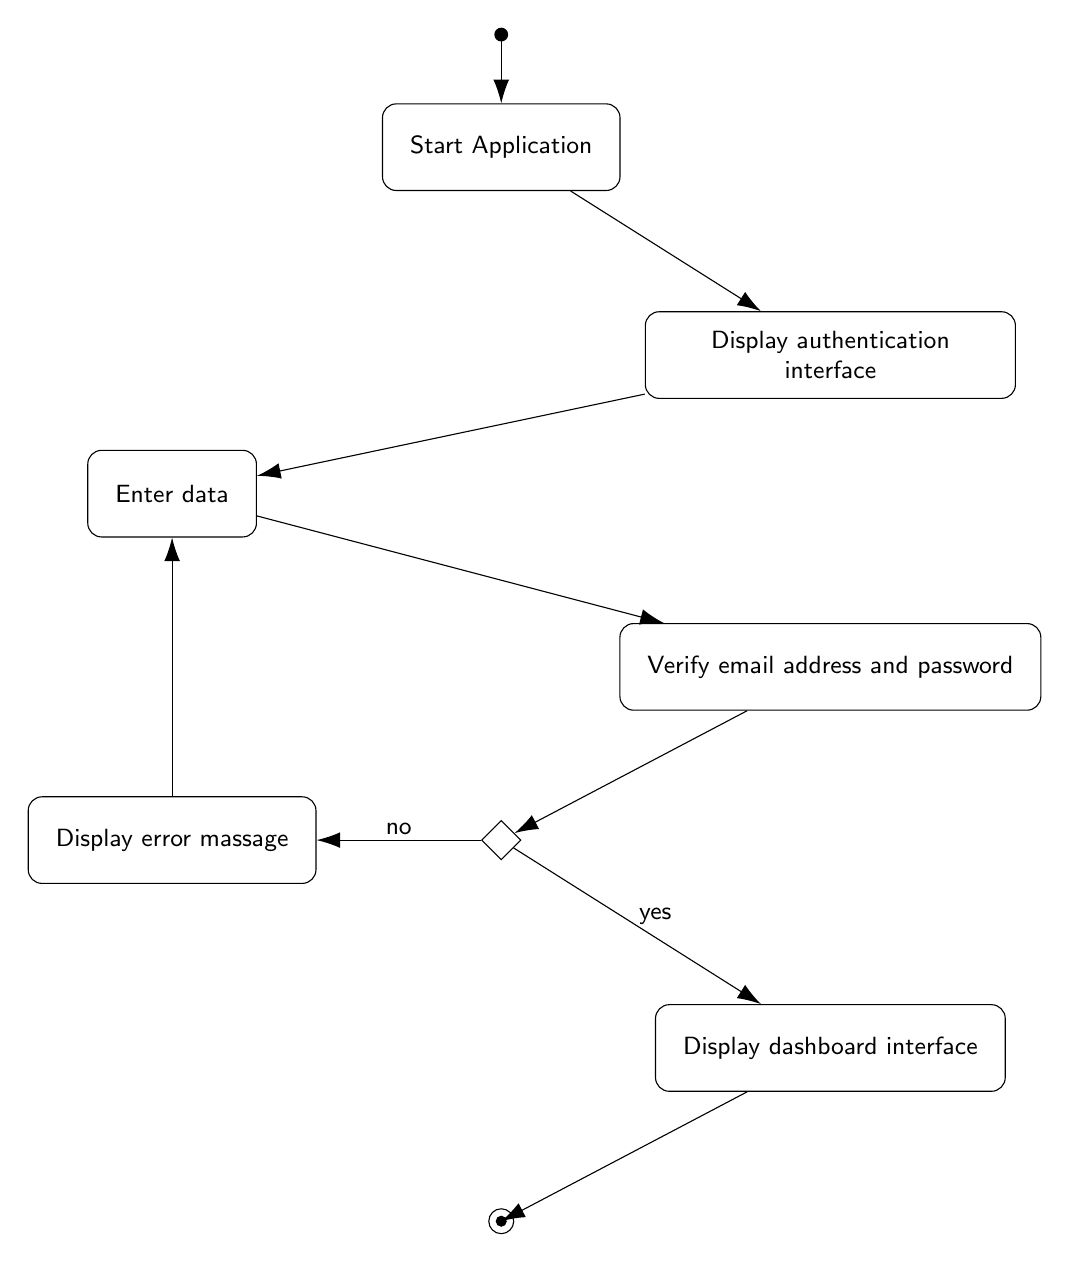
\begin{tikzpicture}[
    x=1.1cm, y=1.1cm,
    box/.style={rectangle, rounded corners=5pt, draw=black, thin,
                minimum height=1.1cm, align=center,
                fill=white, font=\sffamily\small, inner xsep=3.5mm, inner ysep=2mm},
    diamond_node/.style={diamond, draw=black, thin, minimum size=0.5cm, inner sep=0pt},
    arrow/.style={-{Latex[length=3mm, width=2mm]}, thin}
]

% ================= COORDINATES & NODES =================
\coordinate (Start) at (0, 8.5);
\fill (Start) circle (2.5pt);

\node[box] (StartApp) at (0, 7.2) {Start Application};

\node[box, text width=4cm] (Auth) at (3.8, 4.8) {Display authentication\\interface};

\node[box] (Enter) at (-3.8, 3.2) {Enter data};

\node[box] (Verify) at (3.8, 1.2) {Verify email address and password};

\node[diamond_node] (Dia) at (0, -0.8) {};

\node[box] (Error) at (-3.8, -0.8) {Display error massage};

\node[box] (Dash) at (3.8, -3.2) {Display dashboard interface};

\coordinate (End) at (0, -5.2);
\draw[thin] (End) circle (4.5pt);
\fill (End) circle (2pt);

% ================= DRAWING ARROWS =================
\draw[arrow] (Start) -- (StartApp);
\draw[arrow] (StartApp) -- (Auth);
\draw[arrow] (Auth) -- (Enter);
\draw[arrow] (Enter) -- (Verify);
\draw[arrow] (Verify) -- (Dia);
\draw[arrow] (Dia.west) -- node[above, font=\sffamily\small, yshift=-0.5mm] {no} (Error.east);
\draw[arrow] (Error.north) -- (Enter.south);
\draw[arrow] (Dia) -- node[above right, font=\sffamily\small, xshift=-1mm, yshift=-1mm] {yes} (Dash);
\draw[arrow] (Dash) -- (End);

\end{tikzpicture}
}
    \caption{Authentication Activity Diagram}
    \label{fig:activity auth}
\end{figure}

\subsection{Registration Activity Diagram}

This diagram models the patient registration flow, including the existence check for an email address and the creation of a new account when the email is not already used.

\begin{figure}[H]
    \centering
    \resizebox{0.75\textwidth}{!}{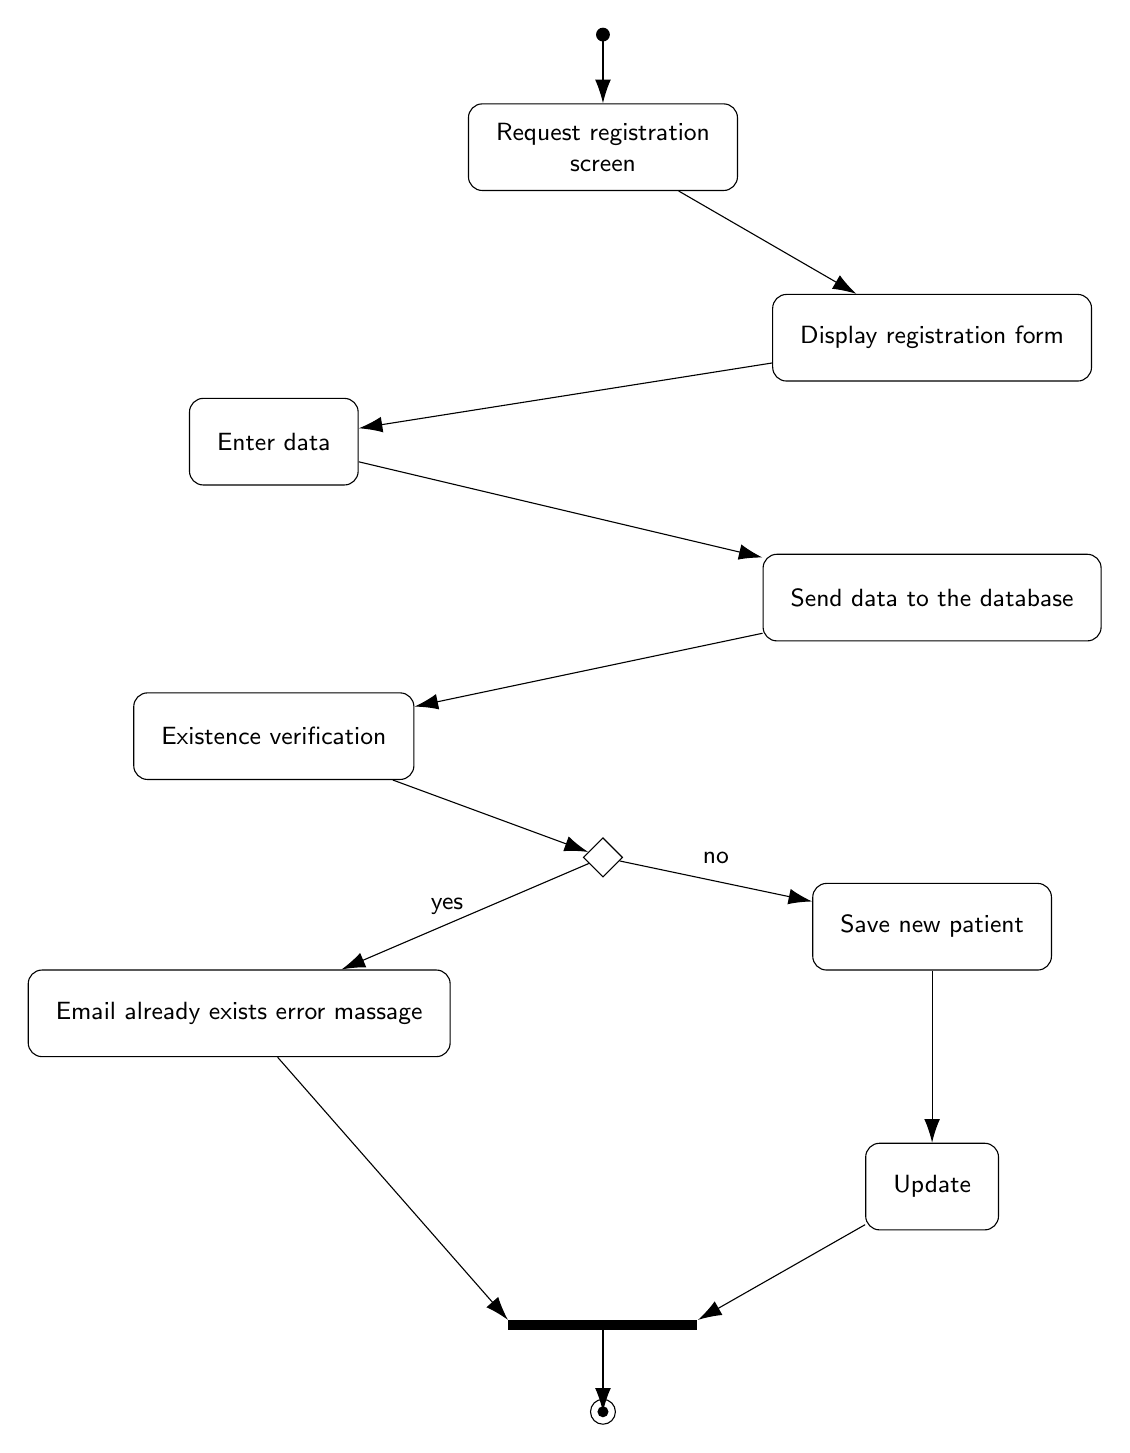
\begin{tikzpicture}[
    x=1.1cm, y=1.1cm,
    box/.style={rectangle, rounded corners=5pt, draw=black, thin,
                minimum height=1.1cm, align=center,
                fill=white, font=\sffamily\small, inner xsep=3.5mm, inner ysep=2mm},
    diamond_node/.style={diamond, draw=black, thin, minimum size=0.5cm, inner sep=0pt},
    bar/.style={rectangle, fill=black, minimum width=2.4cm, minimum height=0.12cm, inner sep=0pt},
    arrow/.style={-{Latex[length=3mm, width=2mm]}, thin}
]

% ================= COORDINATES & NODES =================
% Start Node
\coordinate (Start) at (0, 8.5);
\fill (Start) circle (2.5pt);

% Action Nodes
\node[box] (Req) at (0, 7.2) {Request registration\\screen};
\node[box] (Disp) at (3.8, 5.0) {Display registration form};
\node[box] (Enter) at (-3.8, 3.8) {Enter data};
\node[box] (Send) at (3.8, 2.0) {Send data to the database};
\node[box] (Exist) at (-3.8, 0.4) {Existence verification};

% Decision Diamond
\node[diamond_node] (Dia) at (0, -1.0) {};

% Branches (Preserving the exact spelling from the image)
\node[box] (Error) at (-4.2, -2.8) {Email already exists error massage};
\node[box] (Save) at (3.8, -1.8) {Save new patient};
\node[box] (Update) at (3.8, -4.8) {Update};

% Synchronization Bar (Join Node)
\node[bar] (Join) at (0, -6.4) {};

% End Node
\coordinate (End) at (0, -7.4);
\draw[thin] (End) circle (4.5pt);
\fill (End) circle (2pt);


% ================= DRAWING ARROWS =================
% Main zigzag flow
\draw[arrow] (Start) -- (Req);
\draw[arrow] (Req) -- (Disp);
\draw[arrow] (Disp) -- (Enter);
\draw[arrow] (Enter) -- (Send);
\draw[arrow] (Send) -- (Exist);
\draw[arrow] (Exist) -- (Dia);

% Diamond conditional branches
\draw[arrow] (Dia) -- node[above left, xshift=1mm, yshift=-1mm, font=\sffamily\small] {yes} (Error);
\draw[arrow] (Dia) -- node[above, yshift=1mm, font=\sffamily\small] {no} (Save);

% Vertical continuation
\draw[arrow] (Save) -- (Update);

% Connections hitting the outer edges of the Join bar
\draw[arrow] (Error) -- (Join.north west);
\draw[arrow] (Update) -- (Join.north east);

% Final End arrow
\draw[arrow] (Join.south) -- (End);

\end{tikzpicture}
}
    \caption{Registration Activity Diagram}
    \label{fig:activity reg}
\end{figure}

\subsection{Appointment Booking Activity Diagram}

This diagram illustrates how a patient requests an appointment, how availability is checked, and how the booking is confirmed and persisted.

\begin{figure}[H]
    \centering
    \resizebox{0.75\textwidth}{!}{\input{figures/tikz/activity-book.tex}}
    \caption{Appointment Booking Activity Diagram}
    \label{fig:activity book}
\end{figure}

\subsection{AI Symptom Triage Activity Diagram}

This diagram details the triage workflow where a patient submits symptoms, the system calls the AI service, and the platform presents an urgency assessment and recommended next actions.

\begin{figure}[H]
    \centering
    \resizebox{0.75\textwidth}{!}{\input{figures/tikz/activity-triage.tex}}
    \caption{AI Symptom Triage Activity Diagram}
    \label{fig:activity triage}
\end{figure}

\subsection{PRI Computation Activity Diagram}

This diagram models the computation of the Patient Recovery Index (PRI) by aggregating medication adherence, laboratory trends, engagement signals, and physician evaluation into a single score.

\begin{figure}[H]
    \centering
    \resizebox{0.75\textwidth}{!}{\input{figures/tikz/activity-pri.tex}}
    \caption{PRI Computation Activity Diagram}
    \label{fig:activity pri}
\end{figure}

\section{AI Module Architecture}

DocTIP integrates AI modules distributed between server side Edge Functions (using OpenAI GPT 4) and client side functions (using OpenRouter with the GPT 4.1 nano model).

\begin{figure}[H]
    \centering
    \resizebox{0.94\textwidth}{!}{% DoctIP AI Module Architecture (17 modules)
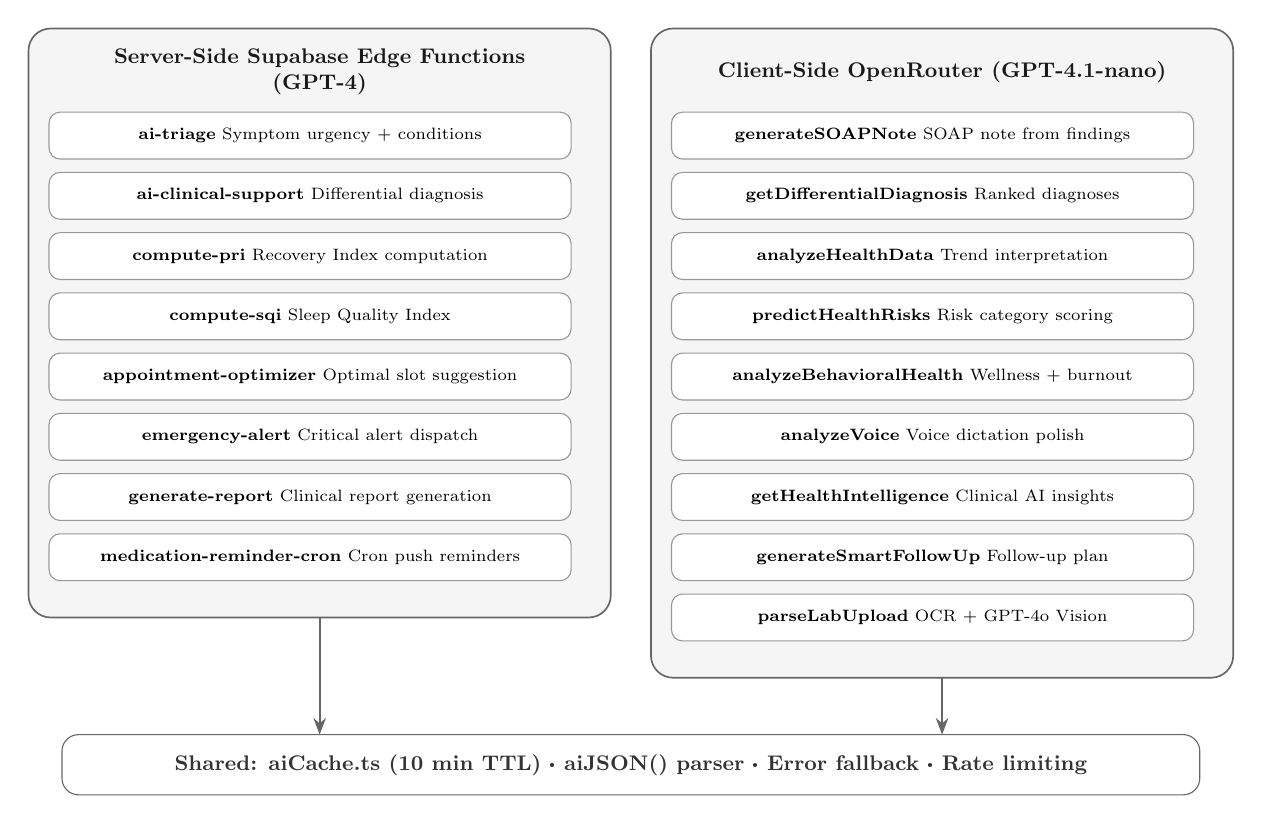
\begin{tikzpicture}[x=1cm,y=1cm, scale=0.85, every node/.style={scale=0.85}]
  \tikzset{
    grp/.style={draw=black!60, fill=black!4, rounded corners=8pt, line width=0.6pt},
    mod/.style={draw=black!40, fill=white, rounded corners=4pt, minimum width=7.8cm, minimum height=0.7cm, align=left, font=\scriptsize, inner sep=5pt},
    mhdr/.style={font=\small\bfseries, text=black!90, align=center},
    arr/.style={-{Stealth[length=6pt]}, black!60, line width=0.8pt},
    infra/.style={draw=black!60, fill=white, rounded corners=6pt, minimum width=17.0cm, minimum height=0.9cm, font=\small\bfseries, text=black!80}
  }

  % - Server-Side Box ---
  % Box spans from X: -4.5 to 4.2
  \draw[grp] (-4.5, 0.8) rectangle (4.2, -8.0);
  \node[mhdr, text width=7.9cm] at (-0.15, 0.15) {Server-Side Supabase Edge Functions\\(GPT-4)};
  
  \node[mod, right] (s1) at (-4.2, -0.8) {\textbf{ai-triage} Symptom urgency + conditions};
  \node[mod, right] (s2) at (-4.2, -1.7) {\textbf{ai-clinical-support} Differential diagnosis};
  \node[mod, right] (s3) at (-4.2, -2.6) {\textbf{compute-pri} Recovery Index computation};
  \node[mod, right] (s4) at (-4.2, -3.5) {\textbf{compute-sqi} Sleep Quality Index};
  \node[mod, right] (s5) at (-4.2, -4.4) {\textbf{appointment-optimizer} Optimal slot suggestion};
  \node[mod, right] (s6) at (-4.2, -5.3) {\textbf{emergency-alert} Critical alert dispatch};
  \node[mod, right] (s7) at (-4.2, -6.2) {\textbf{generate-report} Clinical report generation};
  \node[mod, right] (s8) at (-4.2, -7.1) {\textbf{medication-reminder-cron} Cron push reminders};

  % - Client-Side Box ---
  % Box spans from X: 4.8 to 13.5
  \draw[grp] (4.8, 0.8) rectangle (13.5, -8.9);
  \node[mhdr] at (9.15, 0.15) {Client-Side OpenRouter (GPT-4.1-nano)};

  \node[mod, right] (c1) at (5.1, -0.8) {\textbf{generateSOAPNote} SOAP note from findings};
  \node[mod, right] (c2) at (5.1, -1.7) {\textbf{getDifferentialDiagnosis} Ranked diagnoses};
  \node[mod, right] (c3) at (5.1, -2.6) {\textbf{analyzeHealthData} Trend interpretation};
  \node[mod, right] (c4) at (5.1, -3.5) {\textbf{predictHealthRisks} Risk category scoring};
  \node[mod, right] (c5) at (5.1, -4.4) {\textbf{analyzeBehavioralHealth} Wellness + burnout};
  \node[mod, right] (c6) at (5.1, -5.3) {\textbf{analyzeVoice} Voice dictation polish};
  \node[mod, right] (c7) at (5.1, -6.2) {\textbf{getHealthIntelligence} Clinical AI insights};
  \node[mod, right] (c8) at (5.1, -7.1) {\textbf{generateSmartFollowUp} Follow-up plan};
  \node[mod, right] (c9) at (5.1, -8.0) {\textbf{parseLabUpload} OCR + GPT-4o Vision};

  % - Shared Infrastructure ---
  \node[infra] (infra) at (4.5, -10.2) {Shared: aiCache.ts (10 min TTL) \textperiodcentered{} aiJSON() parser \textperiodcentered{} Error fallback \textperiodcentered{} Rate limiting};

  % - Arrows ---
  \draw[arr] (-0.15, -8.0) -- (-0.15, -9.75);
  \draw[arr] (9.15, -8.9) -- (9.15, -9.75);

\end{tikzpicture}


}
    \caption{Artificial Intelligence Module Architecture}
    \label{fig:ai architecture}
\end{figure}

% Mermaid source: figures/mermaid/ai architecture.mmd

Table~\ref{tab:ai modules} details each AI module with its location, model, and use case.

\begin{table}[H]
\centering
\caption{Artificial Intelligence Module Inventory}
\label{tab:ai modules}
\small
\begin{tabular}{|c|l|l|l|}
\hline
\textbf{\#} & \textbf{Module} & \textbf{Location} & \textbf{Use Case} \\
\hline
1  & ai triage                & Edge Function (GPT 4) & Symptom urgency assessment \\
\hline
2  & ai clinical support      & Edge Function (GPT 4) & Differential diagnosis, interactions \\
\hline
3  & appointment optimizer    & Edge Function (algo)  & Optimal slot suggestion \\
\hline
4  & compute pri              & Edge Function (algo)  & Composite PRI computation \\
\hline
5  & emergency alert          & Edge Function         & Emergency alert dispatch \\
\hline
6  & analyzeHealthTrends      & Client (GPT 4.1 nano) & Longitudinal health analysis \\
\hline
7  & predictHealthRisks       & Client (GPT 4.1 nano) & Predictive risk scores \\
\hline
8  & generateFollowUpPlan     & Client (GPT 4.1 nano) & Intelligent follow up plan \\
\hline
9  & generateSOAPNote         & Client (GPT 4.1 nano) & SOAP note generation \\
\hline
10 & analyzeBehavioralHealth  & Client (GPT 4.1 nano) & Burnout, stress, sleep \\
\hline
11 & rankDifferentialDiagnoses & Client (GPT 4.1 nano) & Confidence ranked diagnosis \\
\hline
12 & analyzeBilling           & Client (GPT 4.1 nano) & Cost estimation \\
\hline
13 & analyzeResearchData      & Client (GPT 4.1 nano) & Anonymized epidemiology \\
\hline
14 & analyzeImage             & Client (GPT 4.1 nano) & Medical image analysis \\
\hline
15 & analyzeVoice             & Client (GPT 4.1 nano) & Voice transcription \\
\hline
16 & aiGenerate               & Client (GPT 4.1 nano) & General AI generation \\
\hline
17 & aiJSON                   & Client (GPT 4.1 nano) & Structured JSON extraction \\
\hline
\end{tabular}
\end{table}

\section*{Conclusion}
\phantomsection
\addcontentsline{toc}{section}{Conclusion}

In this chapter, we presented the complete design of the DocTIP system through several complementary perspectives. The static aspect was illustrated by the class diagram, representing the database tables and their relationships. The dynamic aspect was detailed through use case diagrams (general and 6 refinements), sequence diagrams (5 scenarios: authentication, AI triage, clinical diagnostic assistance, PRI computation, and anomaly detection), and activity diagrams (5 workflows: authentication, registration, appointment booking, AI triage, and PRI computation).

We also presented the AI module architecture distributed between server and client.

The next chapter will mark the implementation phase, where we will present the system architecture, the technologies employed, and the implemented interfaces through annotated screenshots.


% ============================================================================
%                        CHAPTER 3 IMPLEMENTATION
% ============================================================================
\chapterflyleaf{Implementation}
\chapter{Implementation}

\section*{Introduction}
\phantomsection
\addcontentsline{toc}{section}{Introduction}

This final chapter presents the implementation of the DocTIP platform, detailing the system architecture, technological choices, and key engineering challenges. Applying the architectural models defined previously, it showcases the tangible outcomes of the project through annotated workflows of the patient mobile portal, doctor mobile portal, and web administration dashboard.

\section{System Architecture}

The DocTIP architecture is based on a \textbf{serverless} model centered on Supabase, which contrasts with traditional microservices architecture by eliminating the need to manage servers. This architecture presents significant advantages: automatic scaling, usage proportional costs, simplified deployment, and high availability.

The system is composed of three main layers, detailed in Table~\ref{tab:arch layers}:

\begin{table}[H]
\centering
\caption{Technologies Used per Architectural Layer}
\label{tab:arch layers}
\small
\begin{tabular}{|l|p{10cm}|}
\hline
\textbf{Layer} & \textbf{Technologies \& Components} \\
\hline
\textbf{Presentation layer} & Mobile application (Expo/React Native) and web dashboard (React/Vite). \\
\hline
\textbf{Business logic layer} & Supabase Edge Functions (Deno runtime) and client side AI functions (OpenRouter API). \\
\hline
\textbf{Data layer} & PostgreSQL (Supabase) with Row Level Security, Supabase Realtime for real time subscriptions, and Supabase Storage for files. \\
\hline
\end{tabular}
\end{table}

\begin{figure}[H]
    \centering
    \resizebox{0.96\textwidth}{!}{% DoctIP Overall System Architecture (simple scientific diagram)
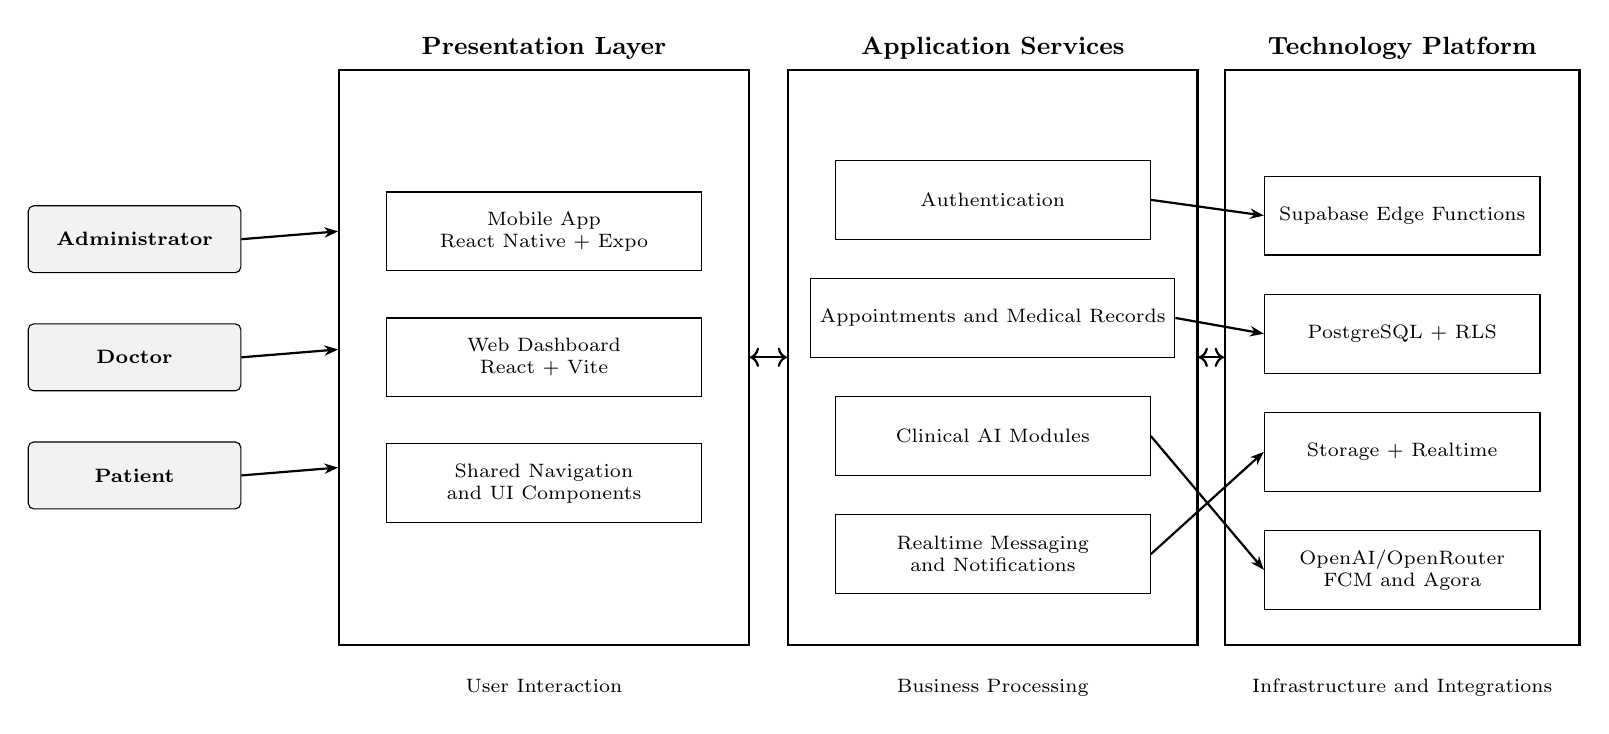
\begin{tikzpicture}[
  font=\small,
  panel/.style={draw, thick, minimum width=5.2cm, minimum height=7.3cm},
  block/.style={draw, minimum width=4.0cm, minimum height=1.0cm, align=center, font=\scriptsize},
  actor/.style={draw, rounded corners=2pt, minimum width=2.7cm, minimum height=0.85cm, align=center, fill=gray!10, font=\scriptsize\bfseries},
  flow/.style={-{Stealth[length=5pt]}, thick},
  bidir/.style={<->, thick},
]
  % Left: system actors
  \node[actor] (admin) at (-8.2,2.2) {Administrator};
  \node[actor] (doctor) at (-8.2,0.7) {Doctor};
  \node[actor] (patient) at (-8.2,-0.8) {Patient};

  % Panel 1: presentation
  \node[panel] (presentation) at (-3.0,0.7) {};
  \node[font=\small\bfseries, anchor=south] at (presentation.north) {Presentation Layer};
  \node[block] (mobile) at (-3.0,2.3) {Mobile App\\React Native + Expo};
  \node[block] (web) at (-3.0,0.7) {Web Dashboard\\React + Vite};
  \node[block] (shared) at (-3.0,-0.9) {Shared Navigation\\and UI Components};

  % Panel 2: core services
  \node[panel] (services) at (2.7,0.7) {};
  \node[font=\small\bfseries, anchor=south] at (services.north) {Application Services};
  \node[block] (auth) at (2.7,2.7) {Authentication};
  \node[block] (clinical) at (2.7,1.2) {Appointments and Medical Records};
  \node[block] (ai) at (2.7,-0.3) {Clinical AI Modules};
  \node[block] (notify) at (2.7,-1.8) {Realtime Messaging\\and Notifications};

  % Panel 3: technology platform
  \node[panel, minimum width=4.5cm] (platform) at (7.9,0.7) {};
  \node[font=\small\bfseries, anchor=south] at (platform.north) {Technology Platform};
  \node[block, minimum width=3.5cm] (edge) at (7.9,2.5) {Supabase Edge Functions};
  \node[block, minimum width=3.5cm] (db) at (7.9,1.0) {PostgreSQL + RLS};
  \node[block, minimum width=3.5cm] (storage) at (7.9,-0.5) {Storage + Realtime};
  \node[block, minimum width=3.5cm] (external) at (7.9,-2.0) {OpenAI/OpenRouter\\FCM and Agora};

  % Inbound actor flows
  \coordinate (p1) at ($(presentation.west)+(0,1.6)$);
  \coordinate (p2) at ($(presentation.west)+(0,0.1)$);
  \coordinate (p3) at ($(presentation.west)+(0,-1.4)$);
  \draw[flow] (admin.east) -- (p1);
  \draw[flow] (doctor.east) -- (p2);
  \draw[flow] (patient.east) -- (p3);

  % Main architecture flow
  \draw[bidir] (presentation.east) -- (services.west);
  \draw[bidir] (services.east) -- (platform.west);

  % Service to platform mappings
  \draw[flow] (auth.east) -- (edge.west);
  \draw[flow] (clinical.east) -- (db.west);
  \draw[flow] (ai.east) -- (external.west);
  \draw[flow] (notify.east) -- (storage.west);

  % Bottom labels
  \node[font=\scriptsize, anchor=north] at ($(presentation.south)+(0,-0.3)$) {User Interaction};
  \node[font=\scriptsize, anchor=north] at ($(services.south)+(0,-0.3)$) {Business Processing};
  \node[font=\scriptsize, anchor=north] at ($(platform.south)+(0,-0.3)$) {Infrastructure and Integrations};
\end{tikzpicture}

}
    \caption{DocTIP Overall System Architecture}
    \label{fig:architecture}
\end{figure}

% Mermaid source: figures/mermaid/system architecture.mmd

\section{Technologies Used}

This section presents the main technologies selected for the project, with a brief justification for each choice based on the requirements identified in Chapter~1. The goal was to keep a coherent stack across mobile, web, backend, and AI features while preserving maintainability and security.

\subsection{Development Tools}

\subsubsection{Visual Studio Code}

\begin{figure}[H]
    \centering
    
\includegraphics[width=0.231\textwidth]{logos/vscode.png}
    \caption{Visual Studio Code Logo}
    \label{fig:logo vscode}
\end{figure}

\textbf{Visual Studio Code} is a free, open source code editor developed by Microsoft, built on the Electron framework. It was used as the primary IDE for TypeScript development, debugging, and extension based workflow.

\subsubsection{Android Studio}

\begin{figure}[H]
    \centering
    
\includegraphics[width=0.231\textwidth]{logos/android-studio.png}
    \caption{Android Studio Logo}
    \label{fig:logo android studio}
\end{figure}

\textbf{Android Studio} is the official integrated development environment (IDE) for Android application development, provided by Google. It provided the Android SDK, emulator, and build toolchain for mobile validation.

\subsection{Frontend Technologies}

\subsubsection{React Native}

\begin{figure}[H]
    \centering
    
\includegraphics[width=0.231\textwidth]{logos/react-native.png}
    \caption{React Native Logo}
    \label{fig:logo react native}
\end{figure}

\textbf{React Native}~\cite{reactnative} enables building native mobile applications using JavaScript/TypeScript and the React component model. The same React component model is reused for the web administration dashboard, ensuring consistency between the mobile and web portals. In DocTIP, React Native powers both the patient and doctor mobile applications, providing a shared codebase for cross platform deployment on iOS and Android with native performance and access to device capabilities.

\subsubsection{Expo}

\begin{figure}[H]
    \centering
    
\includegraphics[width=0.231\textwidth]{logos/expo.png}
    \caption{Expo Logo}
    \label{fig:logo expo}
\end{figure}

\textbf{Expo}~\cite{expo} provides a managed workflow that accelerates development and simplifies access to common device capabilities (camera, GPS, notifications). In DocTIP, Expo handles the build and deployment pipeline, over the air updates, and provides modules for camera access (profile photos, lab result OCR), GPS geolocation (emergency mode, doctor discovery map), and push notifications (appointment reminders, medication alerts).

\textbf{Justification:} The project required a cross platform mobile application with a single codebase, rapid iteration, and stable deployment. React Native and Expo satisfied these constraints while keeping the UI layer consistent with the web dashboard.

\subsubsection{Vite}

\begin{figure}[H]
    \centering
    
\includegraphics[width=0.231\textwidth]{logos/vite.jpeg}
    \caption{Vite Logo}
    \label{fig:logo vite}
\end{figure}

\textbf{Vite}~\cite{vite} offers fast development feedback (HMR) and a modern build pipeline. In DocTIP, Vite powers the web administration dashboard, providing instant hot module replacement during development and optimized production builds for the React based admin interface.

\textbf{Justification:} React was selected for consistency with the mobile portal (shared patterns and developer skills). Vite was chosen to reduce build friction during development.

\subsubsection{Tailwind CSS}

\begin{figure}[H]
    \centering
    
\includegraphics[width=0.231\textwidth]{logos/tailwind.png}
    \caption{Tailwind CSS Logo}
    \label{fig:logo tailwind}
\end{figure}

\textbf{Tailwind CSS}~\cite{tailwind} is a utility first CSS framework that provides pre defined classes for rapid UI development. It was used to style the web administration dashboard, providing consistent spacing, typography, and color schemes across all admin pages including doctor management, patient oversight, analytics, and AI monitoring interfaces.

\textbf{Justification:} Tailwind supports fast UI iteration with consistent spacing and typography while keeping styles predictable across the application.

\subsection{Backend Technologies}

\subsubsection{Supabase}

\begin{figure}[H]
    \centering
    
\includegraphics[width=0.231\textwidth]{logos/supabase.png}
    \caption{Supabase Logo}
    \label{fig:logo supabase}
\end{figure}

\textbf{Supabase}~\cite{supabase} was adopted as the main backend platform. It provides authentication, storage, real time subscriptions, and serverless Edge Functions. In DocTIP, Supabase handles user authentication with role based access control, stores medical records and files in its storage system, enables real time messaging between patients and doctors, and runs server side Edge Functions for AI triage, anomaly detection, and background automation tasks.

\subsubsection{PostgreSQL}

\begin{figure}[H]
    \centering
    
\includegraphics[width=0.231\textwidth]{logos/postgresql.png}
    \caption{PostgreSQL Logo}
    \label{fig:logo postgresql}
\end{figure}

\textbf{PostgreSQL}~\cite{postgresql} is a powerful, open source object relational database management system known for its reliability, feature robustness, and performance. It ensures a robust relational foundation for clinical and operational data. In DocTIP, PostgreSQL stores all platform data including user profiles, medical records, appointments, prescriptions, laboratory results, triage sessions, and recovery scores, with Row Level Security policies ensuring each user can only access their own data.

\textbf{Justification:} This choice reduces backend boilerplate while enabling strong security enforcement through database policies and structured data modeling.

\subsubsection{Deno}

\begin{figure}[H]
    \centering
    
\includegraphics[width=0.231\textwidth]{logos/deno.png}
    \caption{Deno Logo}
    \label{fig:logo deno}
\end{figure}

Server side logic is implemented with Supabase Edge Functions running on the \textbf{Deno} runtime~\cite{deno}, a modern JavaScript and TypeScript runtime built on the V8 engine, designed with security and developer experience in mind. In DocTIP, Deno powers all server side Edge Functions including AI symptom triage, login anomaly detection, appointment optimization, PRI computation, emergency alert dispatch, and background cron jobs for medication reminders.

\textbf{Justification:} Edge Functions support isolated, domain focused endpoints for tasks such as AI requests, background automation, and security checks without maintaining dedicated servers.

\subsection{AI Technologies}

\subsubsection{OpenAI}

\begin{figure}[H]
    \centering
    
\includegraphics[width=0.231\textwidth]{logos/openai.png}
    \caption{OpenAI Logo}
    \label{fig:logo openai}
\end{figure}

\textbf{OpenAI} is an artificial intelligence research organization that develops large language models (GPT 4, GPT 4 Turbo) for natural language understanding and generation. OpenAI models are used for server side clinical support and structured triage. In DocTIP, OpenAI powers the AI symptom triage system that assesses urgency and recommends specialties, generates SOAP clinical notes from voice dictation, and provides differential diagnosis suggestions based on patient symptoms and medical history.

\subsubsection{OpenRouter}

\begin{figure}[H]
    \centering
    
\includegraphics[width=0.38\textwidth]{logos/openrouter.png}
    \caption{OpenRouter Logo}
    \label{fig:logo openrouter}
\end{figure}

\textbf{OpenRouter}~\cite{openai} is a unified API gateway that provides access to multiple AI models from different providers through a single endpoint. It is used as a client side routing layer for selected AI features when appropriate. In DocTIP, OpenRouter provides access to lightweight models (GPT 4.1 nano) for client side AI features including health trend analysis, predictive risk scoring, behavioral health assessment, and the ORION clinical assistant chatbot.

\textbf{Justification:} The AI layer was designed to keep outputs structured, reduce integration fragility, and support responsible handling of medical context.

\subsection{State Management}

\subsubsection{Zustand}

\begin{figure}[H]
    \centering
    
\includegraphics[width=0.231\textwidth]{logos/zaustand.jpeg}
    \caption{Zustand Logo}
    \label{fig:logo zustand}
\end{figure}

\textbf{Zustand}~\cite{zustand} is used for lightweight global state management on the mobile application. In DocTIP, Zustand manages application state across 7 specialized stores including authentication state, patient profile data, medication tracking, appointment scheduling, messaging, and AI session caching, providing a simple and performant alternative to more complex state management solutions.

\textbf{Justification:} Zustand integrates naturally with React hooks and keeps the state layer simple and easy to evolve as features grow.

\clearpage
\section{Presentation of the Mobile Portal: Patient Side}

In this section, we present the main interfaces of the patient mobile application, organized by functional module. Each interface is illustrated with an annotated screenshot and a brief description of its functionality.

% Unified screenshot sizing rules for Chapter 3 UI figures.
\newcommand{\uiMobileShot}[1]{%
    \includegraphics[width=0.42\textwidth,height=0.70\textheight,keepaspectratio]{#1}%
}
\newcommand{\uiFlowShot}[1]{%
    \includegraphics[width=0.92\textwidth,height=0.58\textheight,keepaspectratio]{#1}%
}
\newcommand{\uiWebShot}[1]{%
    \includegraphics[width=0.96\textwidth,height=0.62\textheight,keepaspectratio]{#1}%
}

\subsection{Authentication and Onboarding}

The authentication flow comprises a role selection screen (patient or doctor), a login screen, and a registration screen. Upon first registration, the patient is guided through a \textbf{4 step onboarding wizard} that collects personal information, medical history, allergies, and lifestyle data. This data is persisted in the \texttt{medical\_records} table and serves as the foundation for all subsequent AI analyses.

The implemented security mechanisms for authentication and access control are as follows:
\begin{enumerate}
    \item \textbf{JWT Authentication:} Tokens signed by Supabase Auth with automatic refresh. Secure storage via AsyncStorage (mobile) or localStorage (web).
    \item \textbf{Row Level Security (RLS):} Every table has row level security policies. A patient can only access their own data. A doctor can only access data of their linked patients.
    \item \textbf{Anomaly Detection:} The Edge Function \texttt{check login anomaly} analyzes each login attempt across 4 criteria: multiple failed attempts (+40 points), new device (+15), new geographic location (+25), unusual time (+10).
    \item \textbf{Risk Scoring:} Cumulative score from 0 to 100. ``allow'' action for scores $< 30$, ``warn\_user'' for 30 to 49, ``require\_2fa'' for $\geq 50$.
    \item \textbf{Alert Notifications:} Automatic alert to the user for scores $\geq 30$, alert to all administrators for scores $\geq 50$.
\end{enumerate}

\begin{figure}[H]
    \centering
    \begin{minipage}{0.30\textwidth}
        \centering
        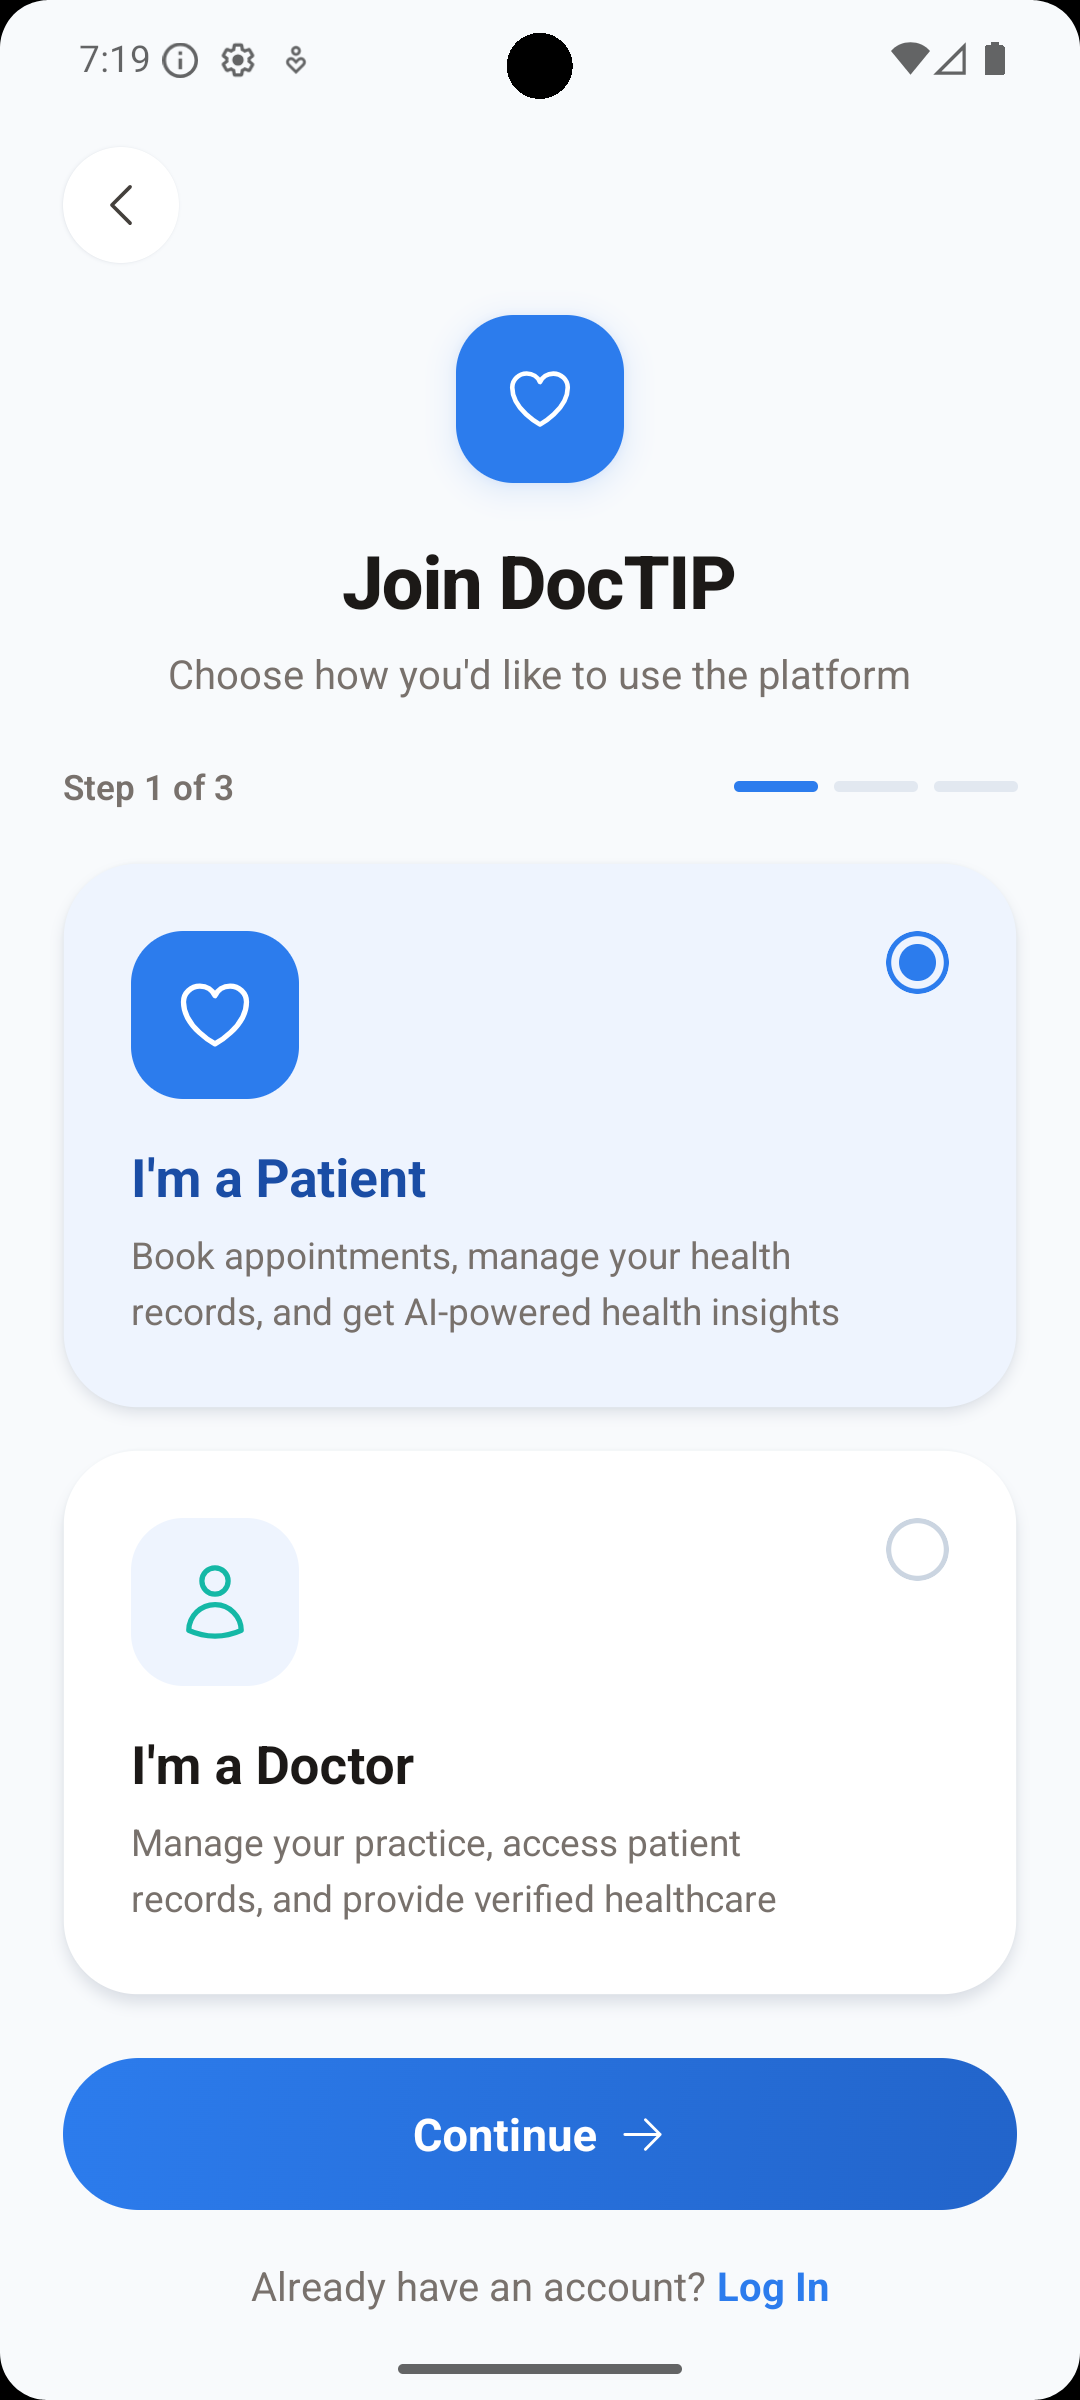
\includegraphics[width=\textwidth,height=0.70\textheight,keepaspectratio]{patientregistre.png}
    \end{minipage}\hfill
    \begin{minipage}{0.30\textwidth}
        \centering
        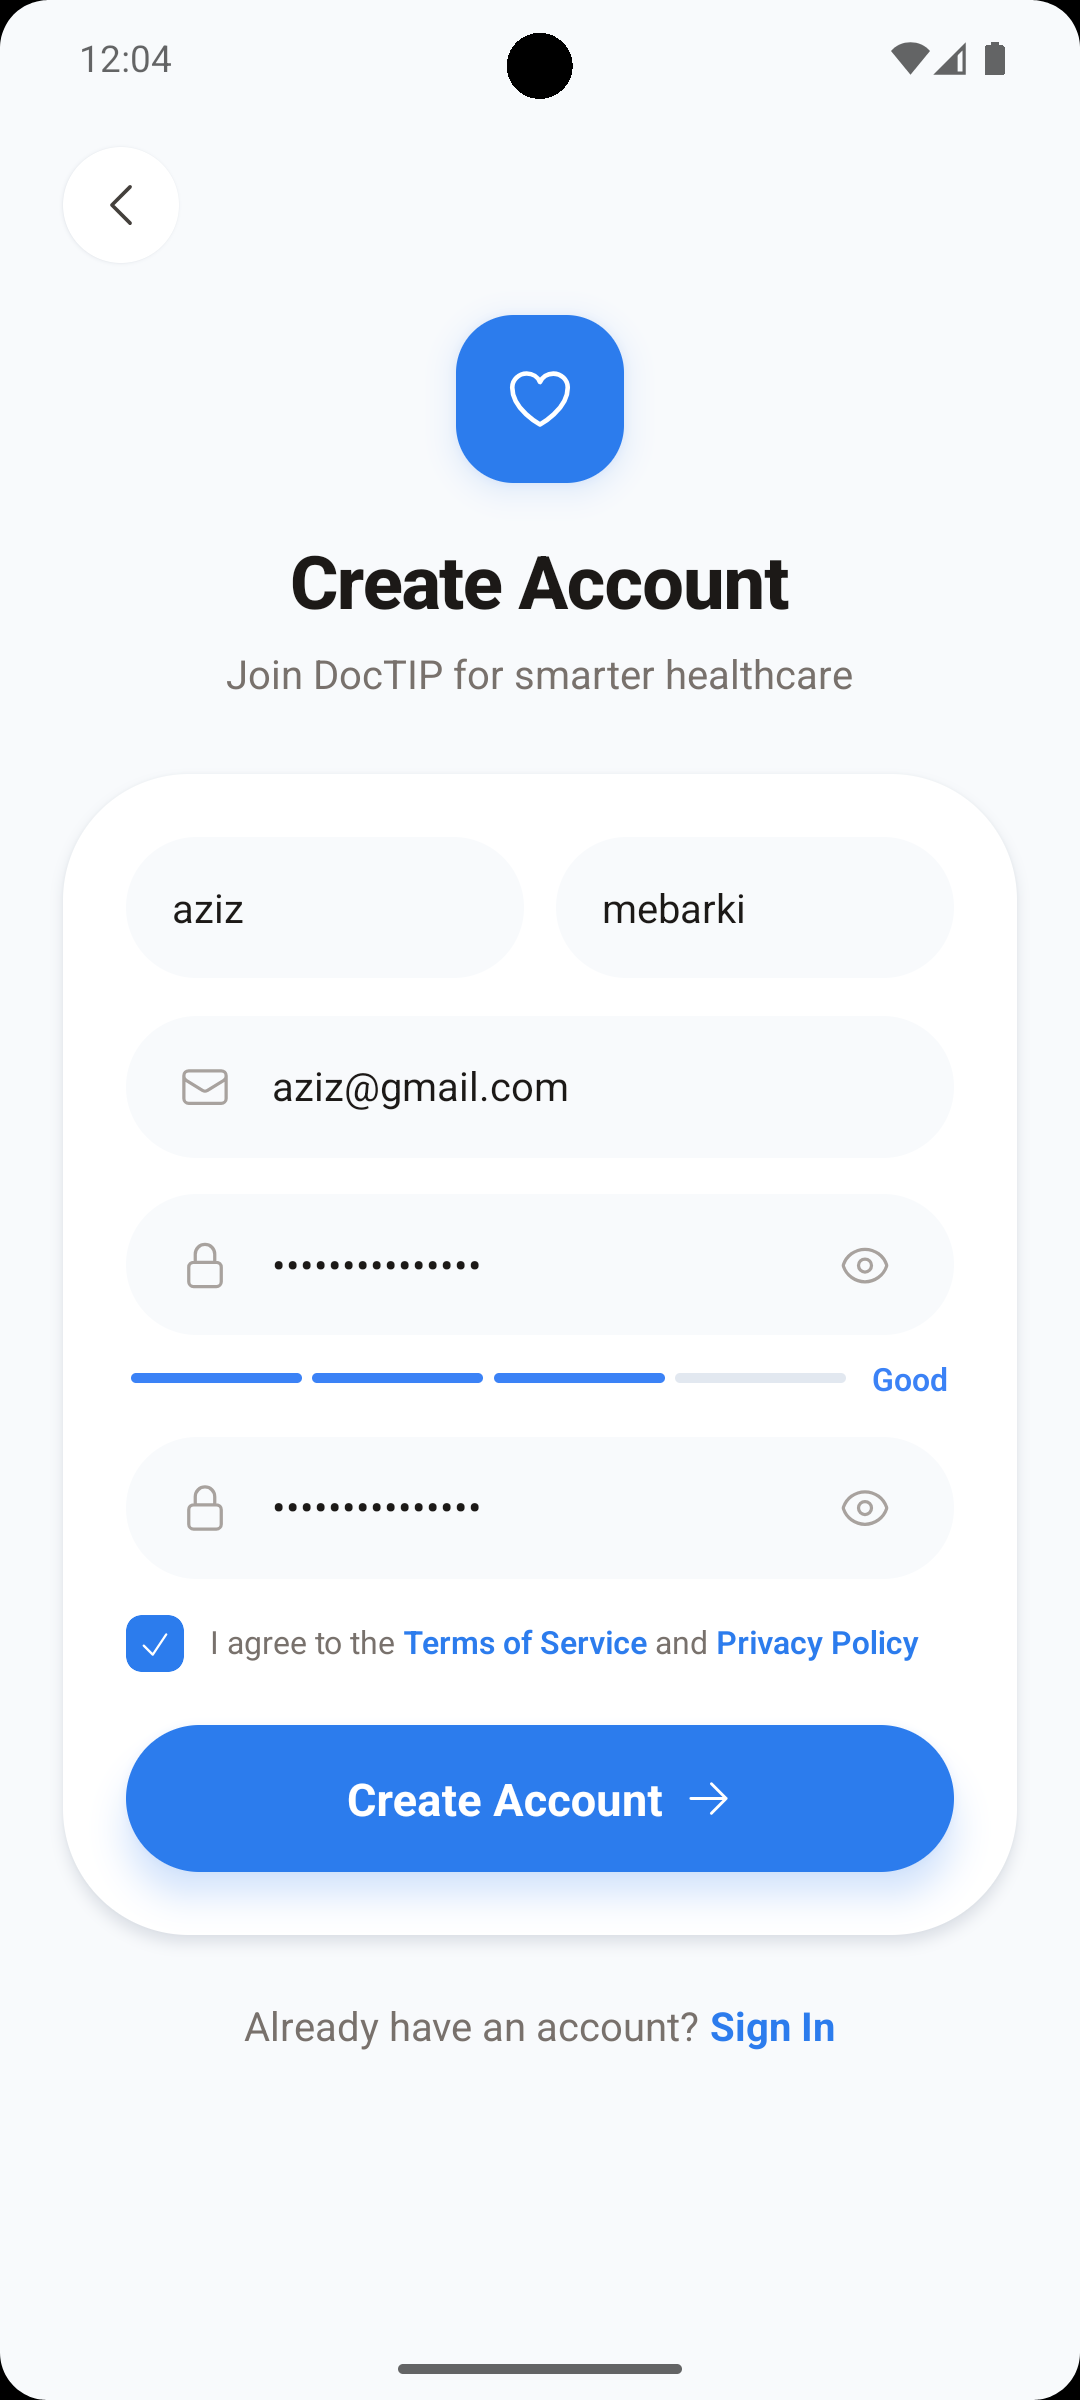
\includegraphics[width=\textwidth,height=0.70\textheight,keepaspectratio]{screen-auth-flow.png}
    \end{minipage}\hfill
    \begin{minipage}{0.30\textwidth}
        \centering
        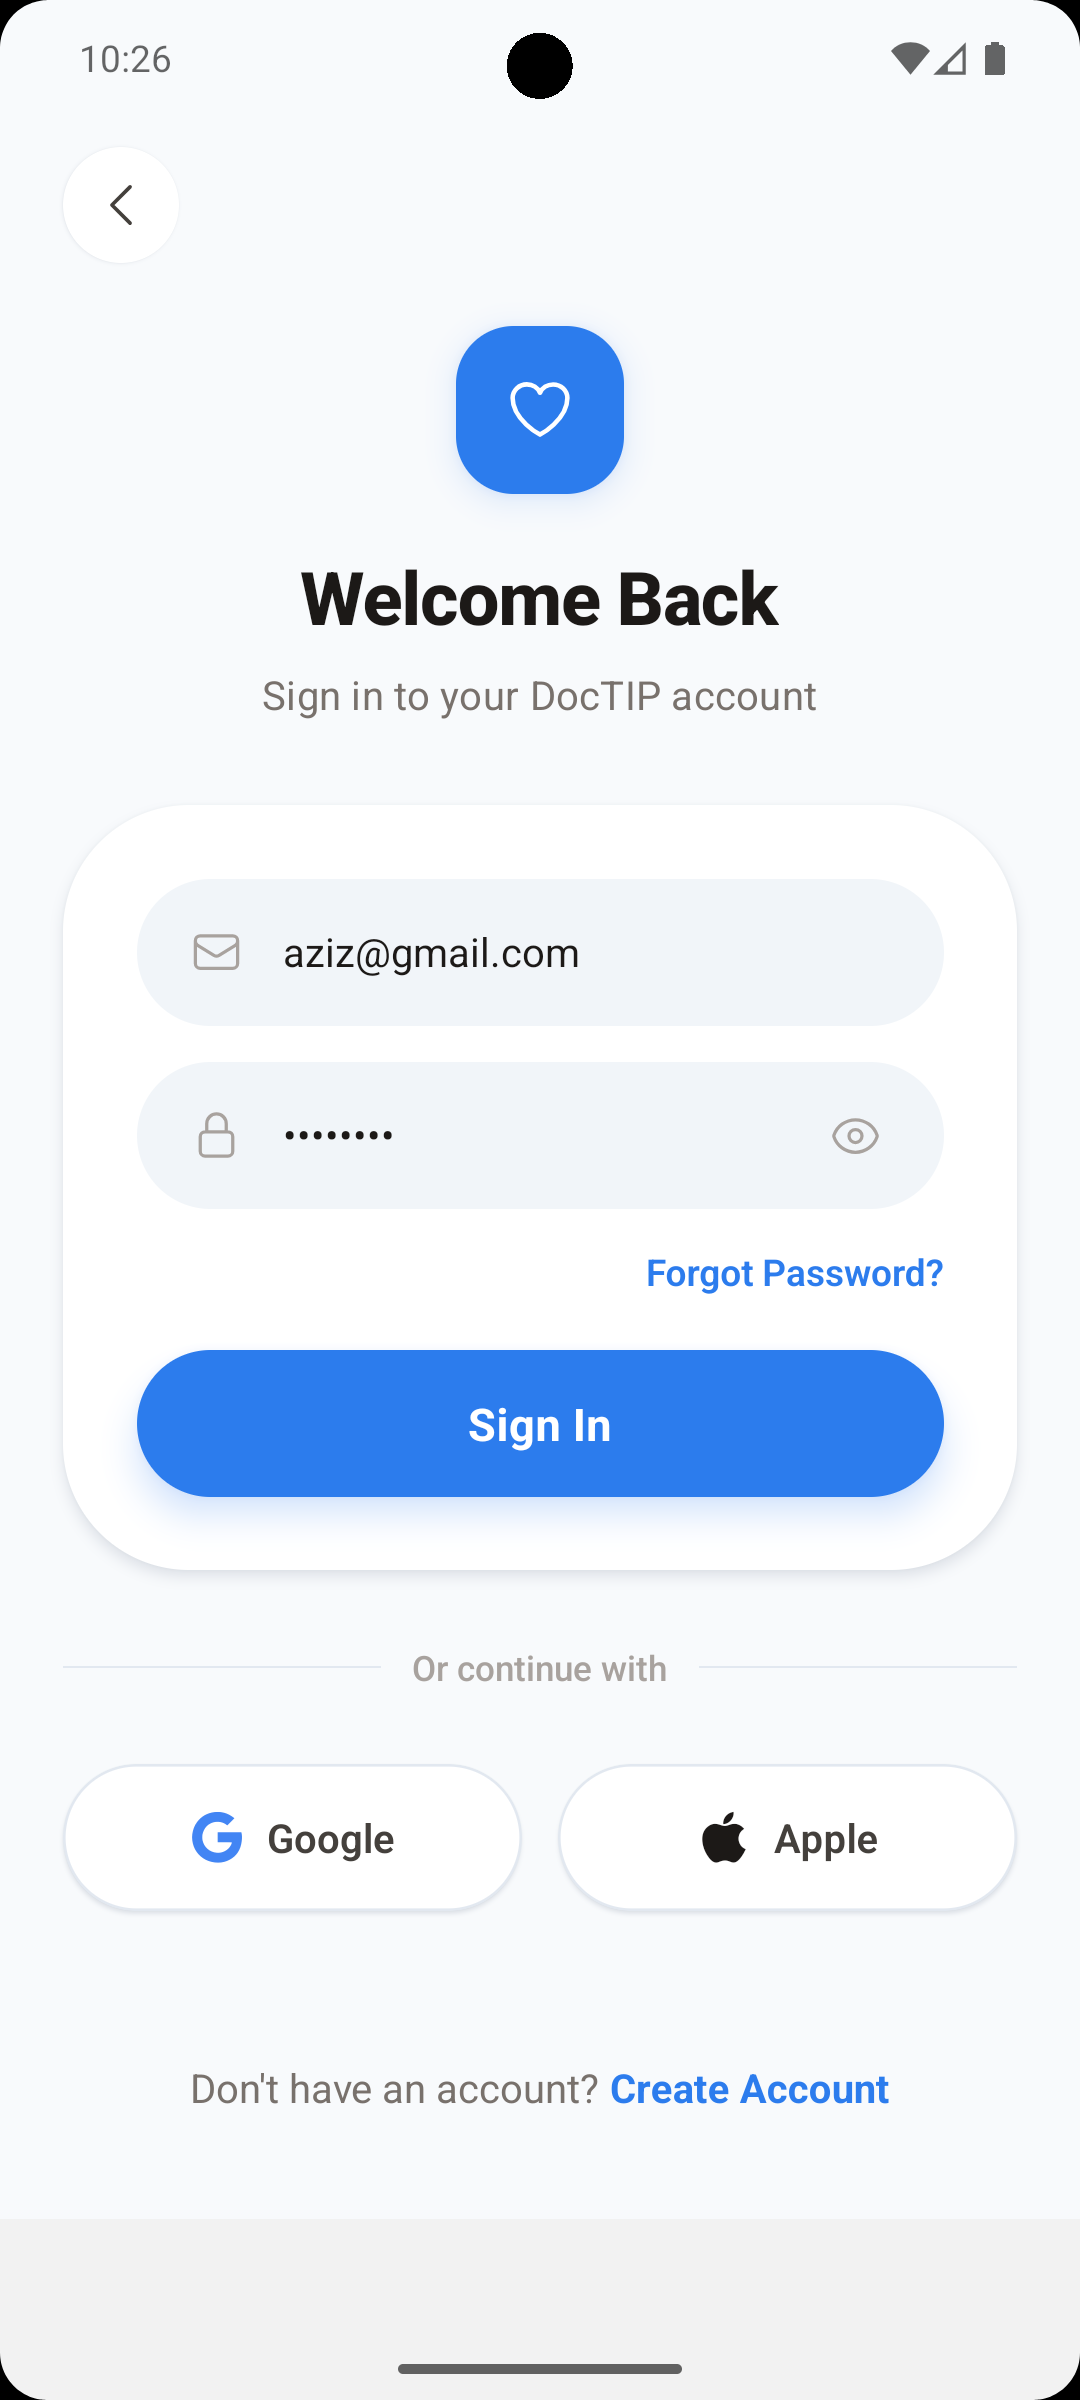
\includegraphics[width=\textwidth,height=0.70\textheight,keepaspectratio]{patientlogin.png}
    \end{minipage}
    \caption{Authentication Flow: Role Selection, Login, and Registration}
    \label{fig:screen auth}
\end{figure}

\subsection{Patient Home Dashboard}

The patient home screen (Figure~\ref{fig:screen patient home}) is the central hub of the patient experience. It features:

\begin{itemize}
    \item A \textbf{weekly calendar strip} with interactive day pills, highlighting the current day in blue with a glow shadow.
    \item A personalized \textbf{greeting header} with the patient's avatar and time based salutation (Good Morning / Afternoon / Evening).
    \item An \textbf{AI powered health insight card} generated via OpenRouter, cached for 10~minutes to minimize API costs.
    \item \textbf{Quick action buttons} for booking appointments, accessing medical records, managing medications, and launching AI triage.
    \item An \textbf{upcoming appointments section} with doctor avatar, specialty, visit type badge, and date.
    \item A \textbf{medication reminder section} showing today's medications with adherence progress ring (taken/missed/pending).
    \item Trend charts with cubic B\'ezier smoothing for health metric visualization.
\end{itemize}

\begin{figure}[H]
    \centering
    \begin{minipage}{0.42\textwidth}
        \centering
        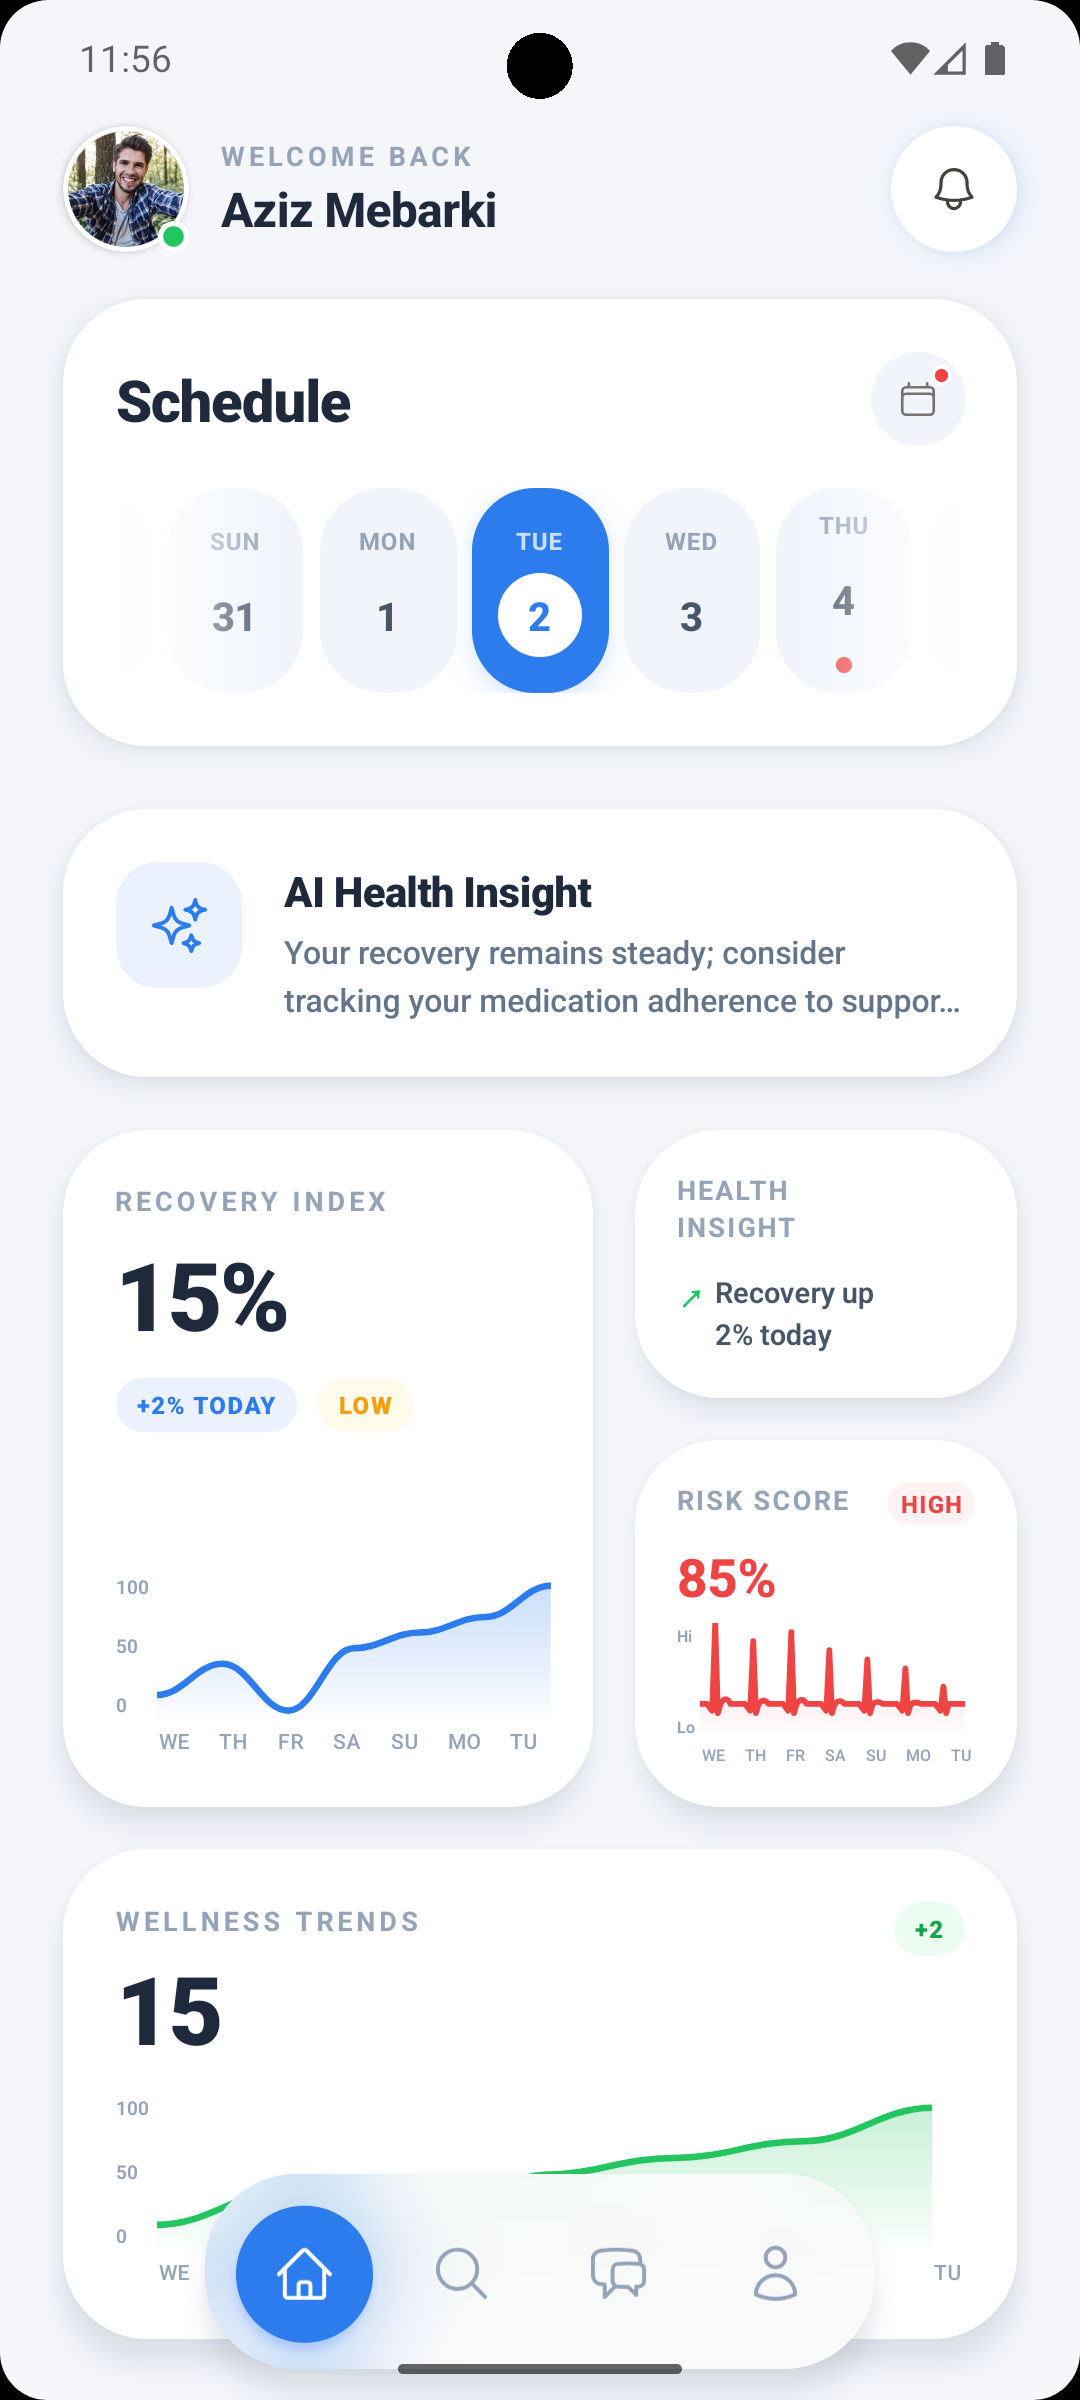
\includegraphics[width=\textwidth,height=0.70\textheight,keepaspectratio]{screen-patient-home.png}
    \end{minipage}\hfill
    \begin{minipage}{0.42\textwidth}
        \centering
        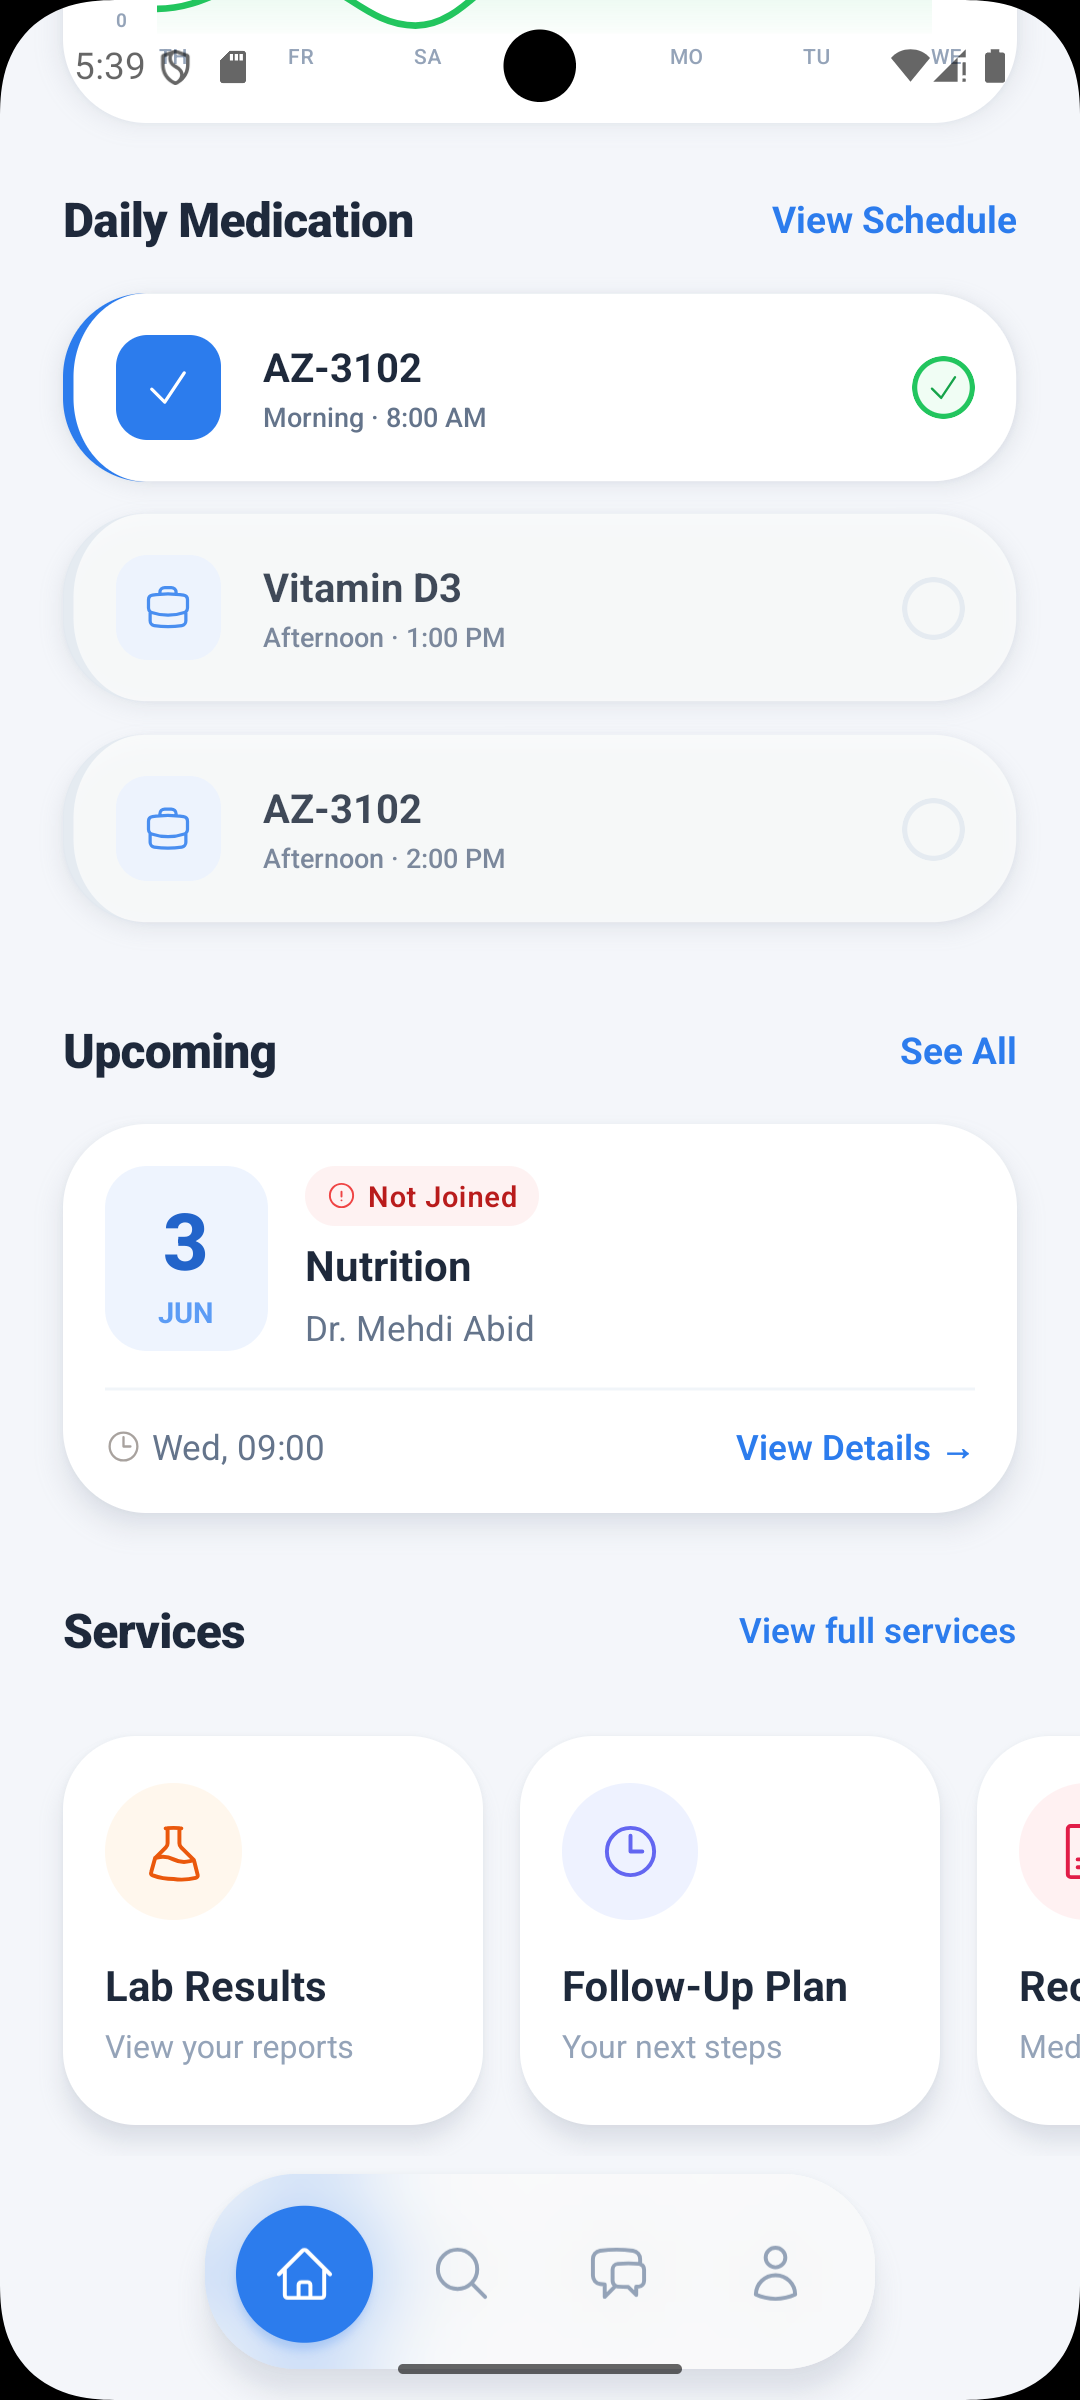
\includegraphics[width=\textwidth,height=0.70\textheight,keepaspectratio]{patienthomedashboard.png}
    \end{minipage}
    \caption{Patient Home Dashboard}
    \label{fig:screen patient home}
\end{figure}

\subsection{AI Symptom Triage}

The triage screen provides a \textbf{conversational AI interface} where the patient describes their symptoms in natural language. The system calls the \texttt{ai triage} Edge Function (GPT 4) which returns:

\begin{itemize}
    \item An \textbf{urgency assessment} (low, moderate, high, emergency) with a color coded badge.
    \item A list of \textbf{possible conditions} ranked by likelihood.
    \item A \textbf{recommended medical specialty} for follow up.
    \item \textbf{Follow up questions} for multi turn conversation refinement.
    \item An \textbf{action plan} with immediate, short term, and long term recommendations.
\end{itemize}

The triage session is persisted in the \texttt{triage\_sessions} table and can be reviewed by the patient's doctor for clinical context.

\begin{figure}[H]
    \centering
    \begin{minipage}{0.42\textwidth}
        \centering
        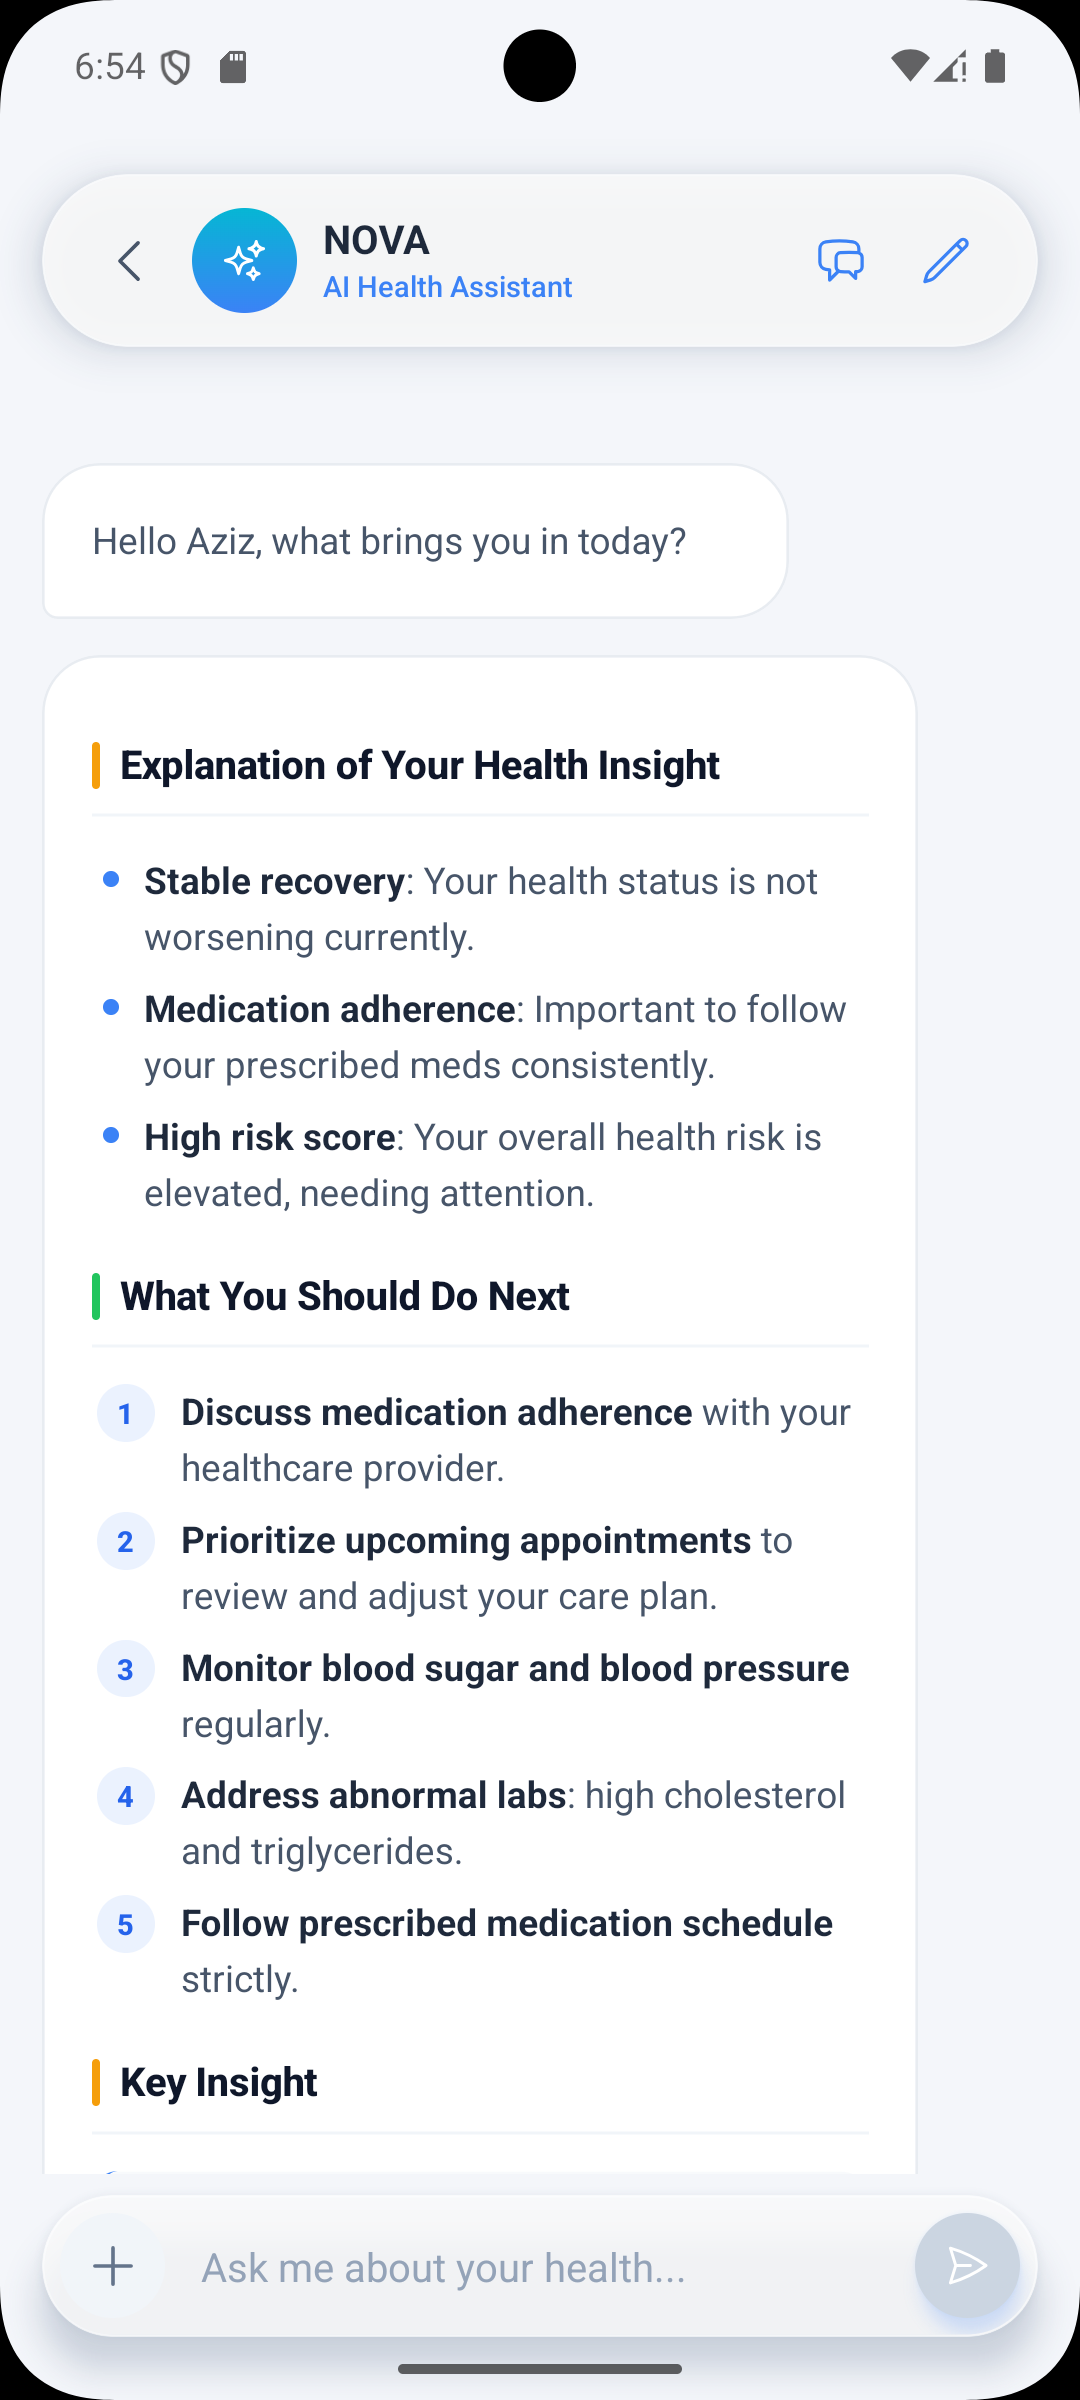
\includegraphics[width=\textwidth,height=0.70\textheight,keepaspectratio]{screen-triage.png}
    \end{minipage}\hfill
    \begin{minipage}{0.42\textwidth}
        \centering
        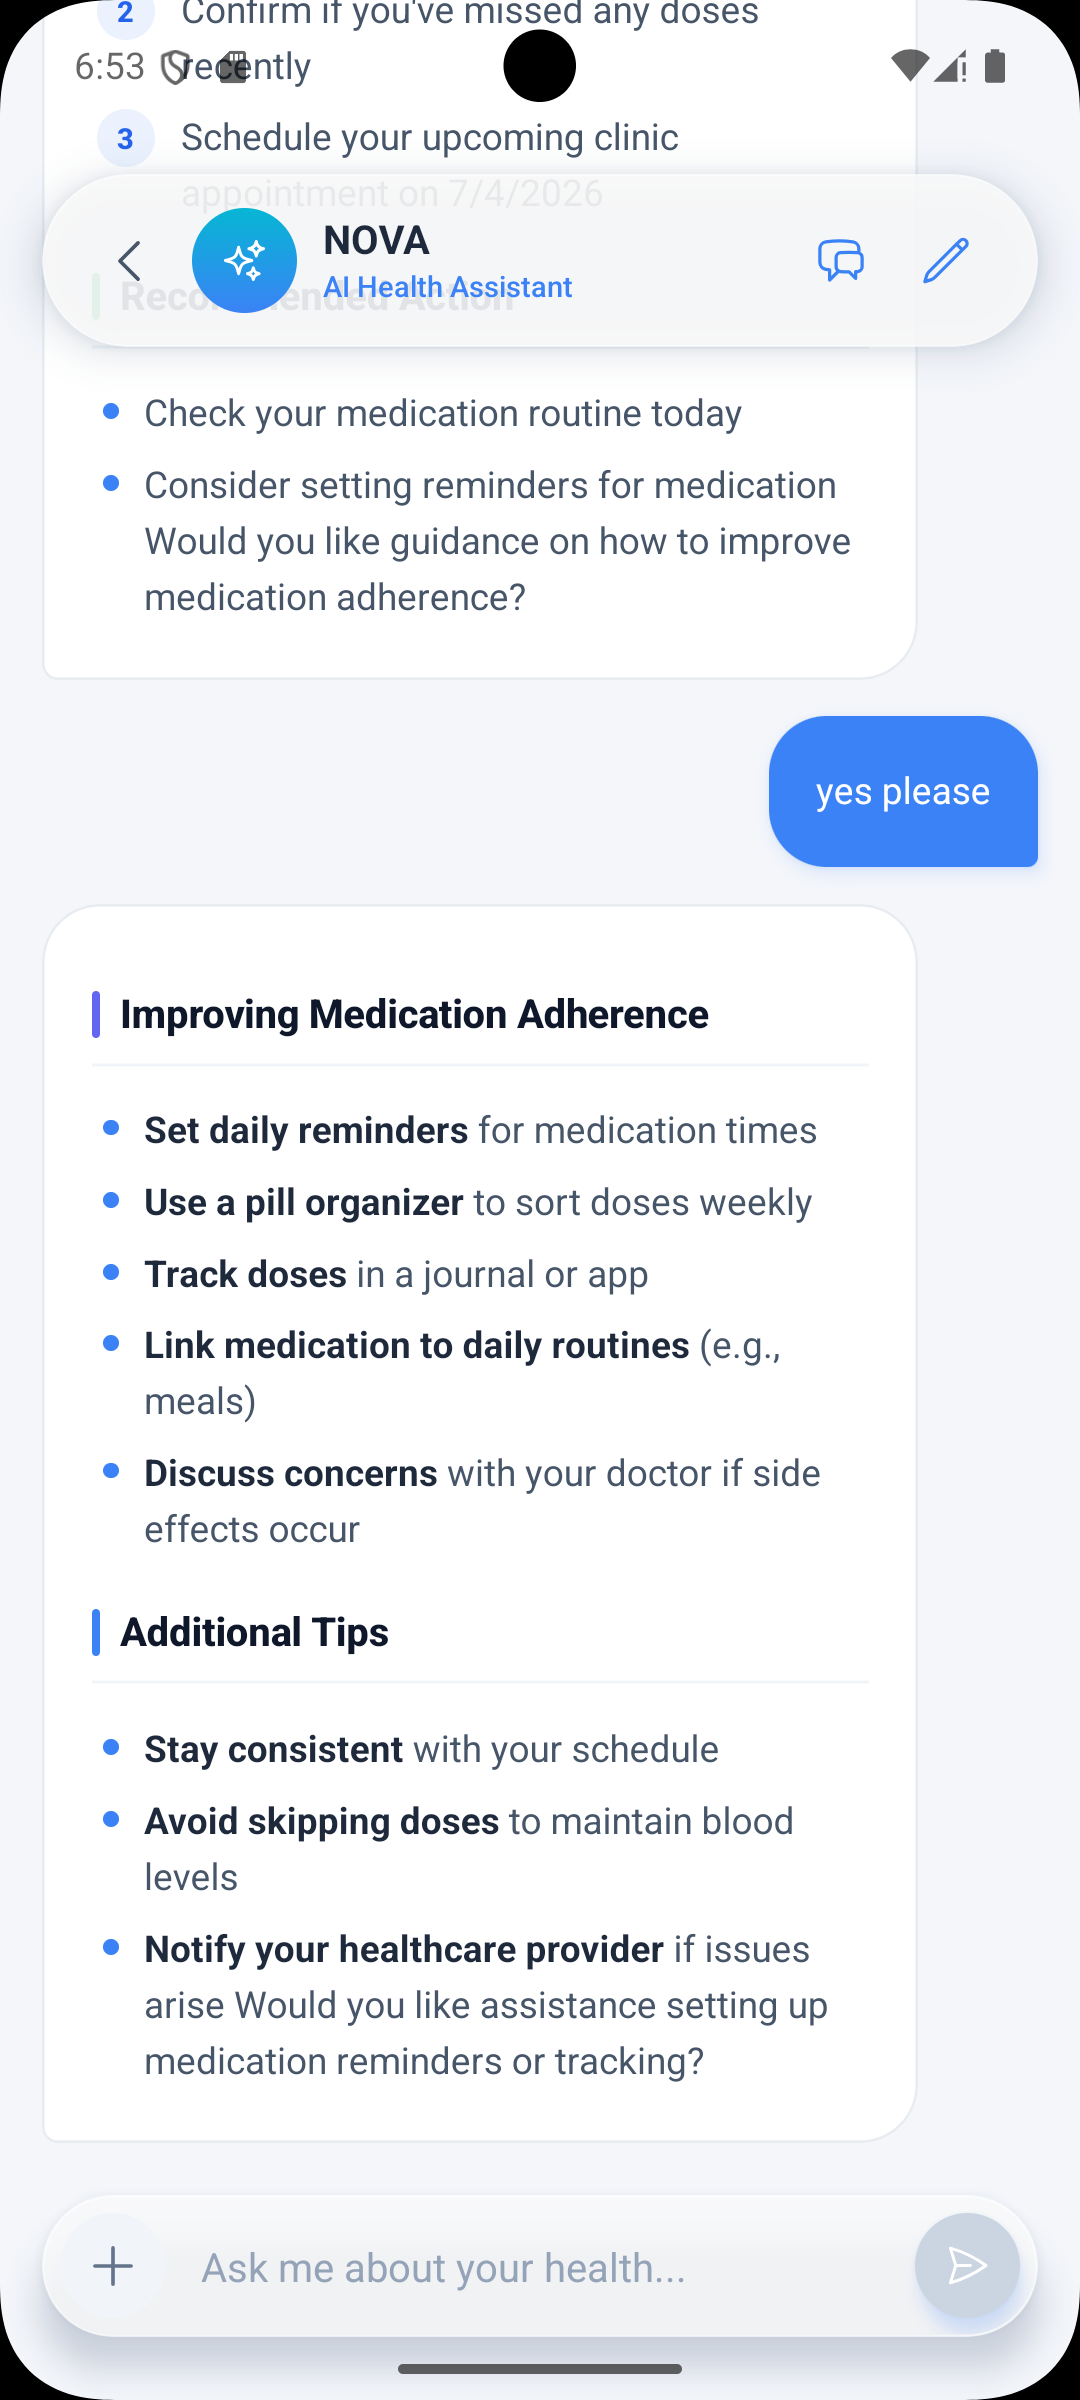
\includegraphics[width=\textwidth,height=0.70\textheight,keepaspectratio]{chat2.png}
    \end{minipage}
    \caption{AI Symptom Triage Interface}
    \label{fig:screen triage}
\end{figure}

\subsection{Appointment Booking}

The first step in the appointment process is discovering a suitable doctor. The patient browses the doctor list, filterable by specialty across 16~categories, with an interactive Leaflet map view showing nearby practitioners. Each doctor card displays their specialty, consultation fees, patient rating, and availability status. Tapping a doctor opens their detailed profile with biography, office location, schedule, and patient reviews. Figure~\ref{fig:screen discover doctor} illustrates the doctor discovery flow.

\begin{figure}[H]
    \centering
    \begin{minipage}{0.32\textwidth}
        \centering
        \IfFileExists{figures/discover1.png}{\uiFlowShot{discover1.png}}{\fcolorbox{black!20}{black!5}{\parbox[c][5.4cm][c]{0.30\textwidth}{\centering\small\itshape\color{black!50}[screenshot: discover1.png]}}}
    \end{minipage}\hfill
    \begin{minipage}{0.32\textwidth}
        \centering
        \IfFileExists{figures/discover2.png}{\uiFlowShot{discover2.png}}{\fcolorbox{black!20}{black!5}{\parbox[c][5.4cm][c]{0.30\textwidth}{\centering\small\itshape\color{black!50}[screenshot: discover2.png]}}}
    \end{minipage}\hfill
    \begin{minipage}{0.32\textwidth}
        \centering
        \IfFileExists{figures/discover3.png}{\uiFlowShot{discover3.png}}{\fcolorbox{black!20}{black!5}{\parbox[c][5.4cm][c]{0.30\textwidth}{\centering\small\itshape\color{black!50}[screenshot: discover3.png]}}}
    \end{minipage}
    \caption{Discover Doctor Flow}
    \label{fig:screen discover doctor}
\end{figure}

Once a doctor is selected, the booking flow proceeds through several steps: selecting a visit type (clinic, home, video) from the doctor's profile, choosing a date from an interactive calendar, and confirming the time slot. The system integrates the \texttt{appointment optimizer} Edge Function to suggest optimal time slots based on doctor availability and patient scheduling patterns. Figure~\ref{fig:screen booking} presents the booking flow after the doctor has been selected.

\begin{figure}[H]
    \centering
    \begin{minipage}{0.32\textwidth}
        \centering
        \IfFileExists{figures/doctorprofile.png}{\uiFlowShot{doctorprofile.png}}{\fcolorbox{black!20}{black!5}{\parbox[c][5.4cm][c]{0.30\textwidth}{\centering\small\itshape\color{black!50}[screenshot: doctorprofile.png]}}}
    \end{minipage}\hfill
    \begin{minipage}{0.32\textwidth}
        \centering
        \IfFileExists{figures/book3.png}{\uiFlowShot{book3.png}}{\fcolorbox{black!20}{black!5}{\parbox[c][5.4cm][c]{0.30\textwidth}{\centering\small\itshape\color{black!50}[screenshot: book3.png]}}}
    \end{minipage}\hfill
    \begin{minipage}{0.32\textwidth}
        \centering
        \IfFileExists{figures/book2.png}{\uiFlowShot{book2.png}}{\fcolorbox{black!20}{black!5}{\parbox[c][5.4cm][c]{0.30\textwidth}{\centering\small\itshape\color{black!50}[screenshot: book2.png]}}}
    \end{minipage}
    \caption{Appointment Booking Flow: Profile, Date Selection}
    \label{fig:screen booking}
\end{figure}

\subsection{Medical Record}

The medical record screen displays the patient's complete health profile including blood type, height, weight, chronic diseases, allergies, surgical history, family history, and lifestyle information. The patient can view and update all health data at any time from a structured multi section interface.

\begin{figure}[H]
    \centering
    \begin{minipage}{0.42\textwidth}
        \centering
        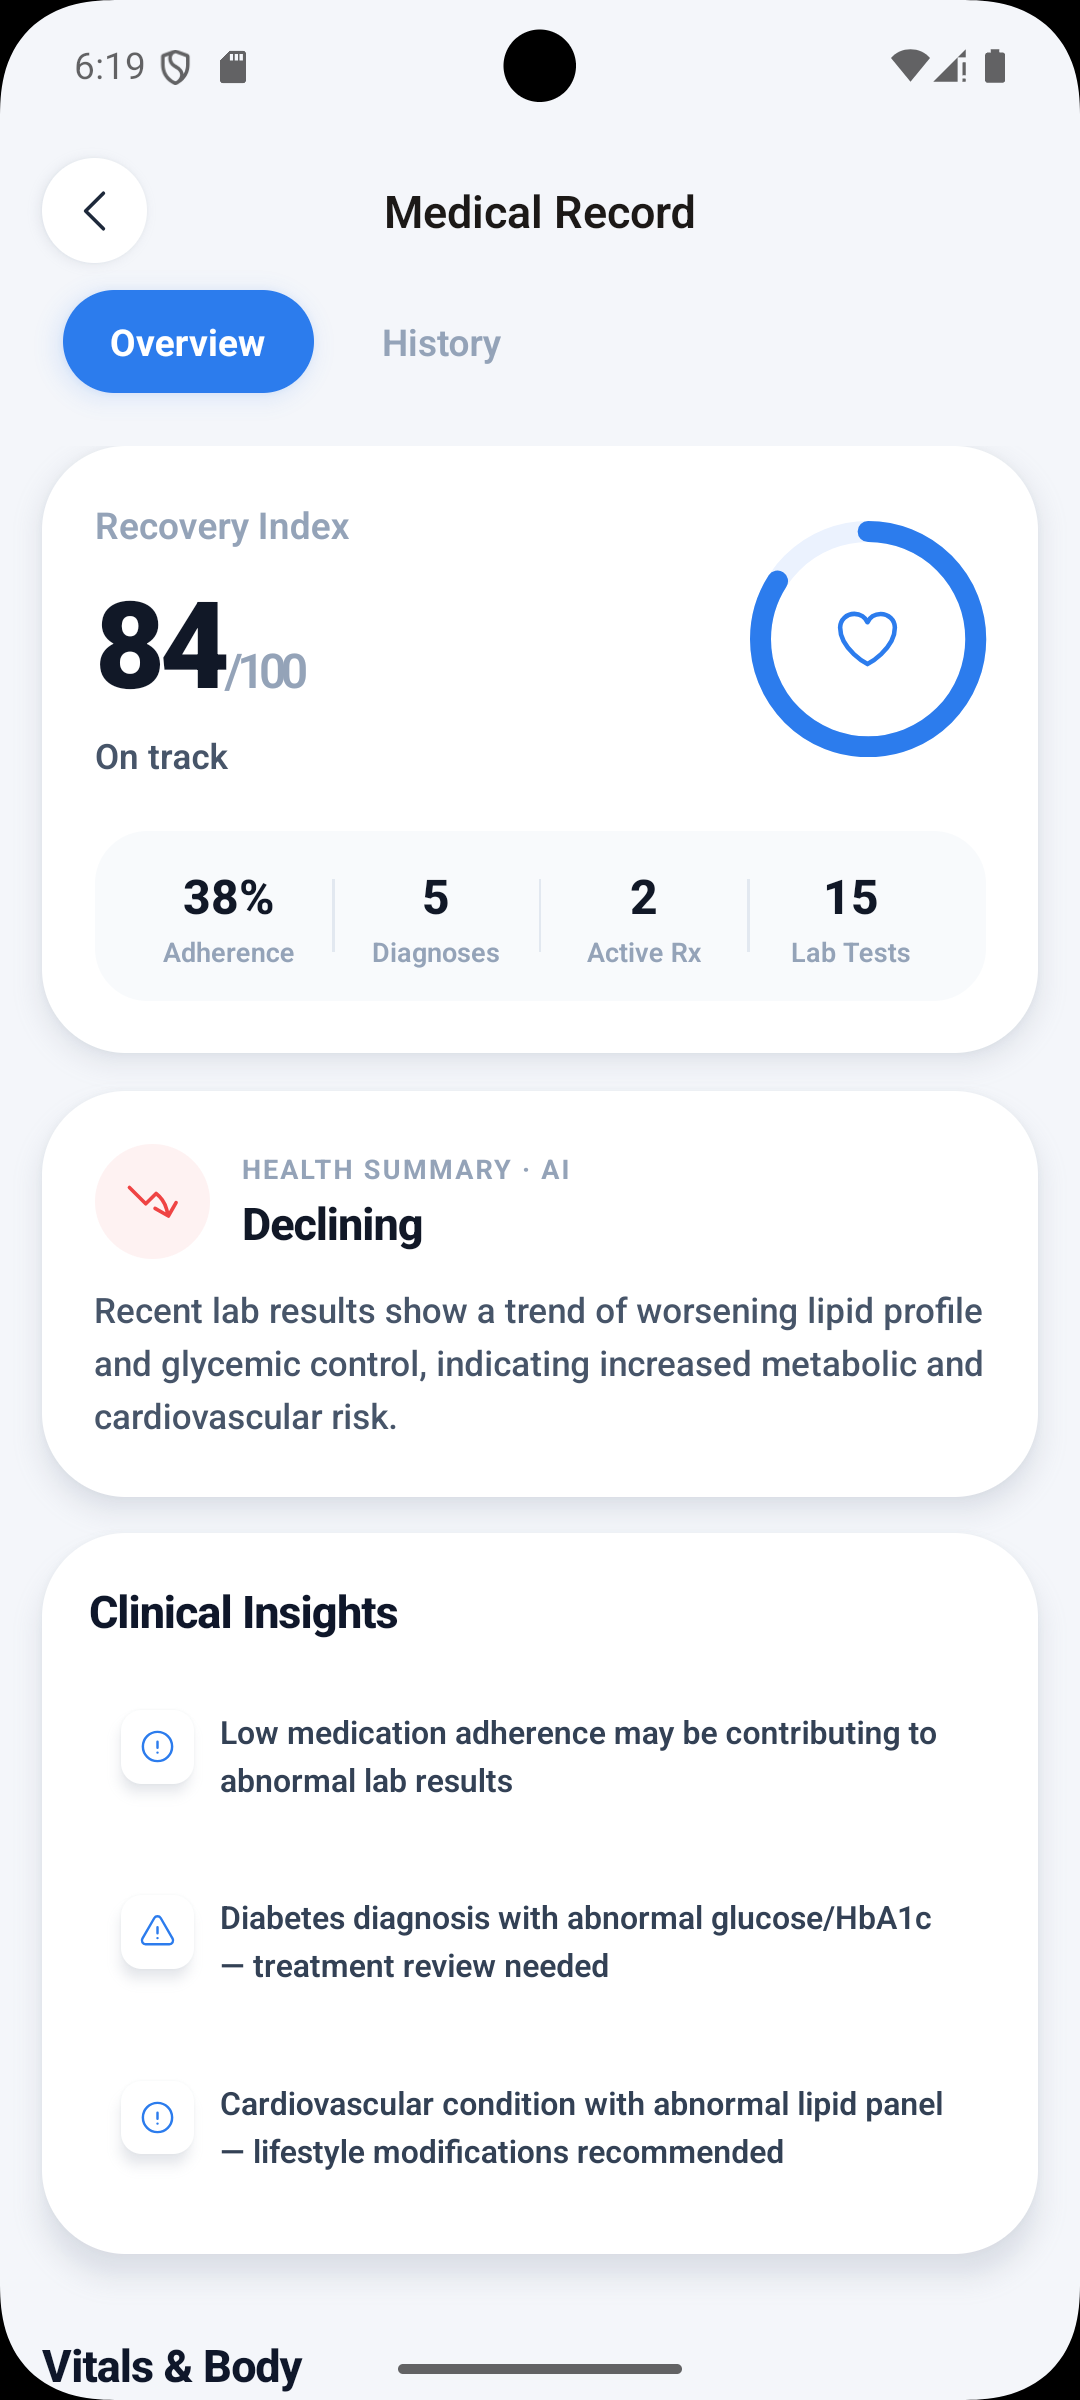
\includegraphics[width=\textwidth,height=0.70\textheight,keepaspectratio]{medicalrecord1.png}
    \end{minipage}\hfill
    \begin{minipage}{0.42\textwidth}
        \centering
        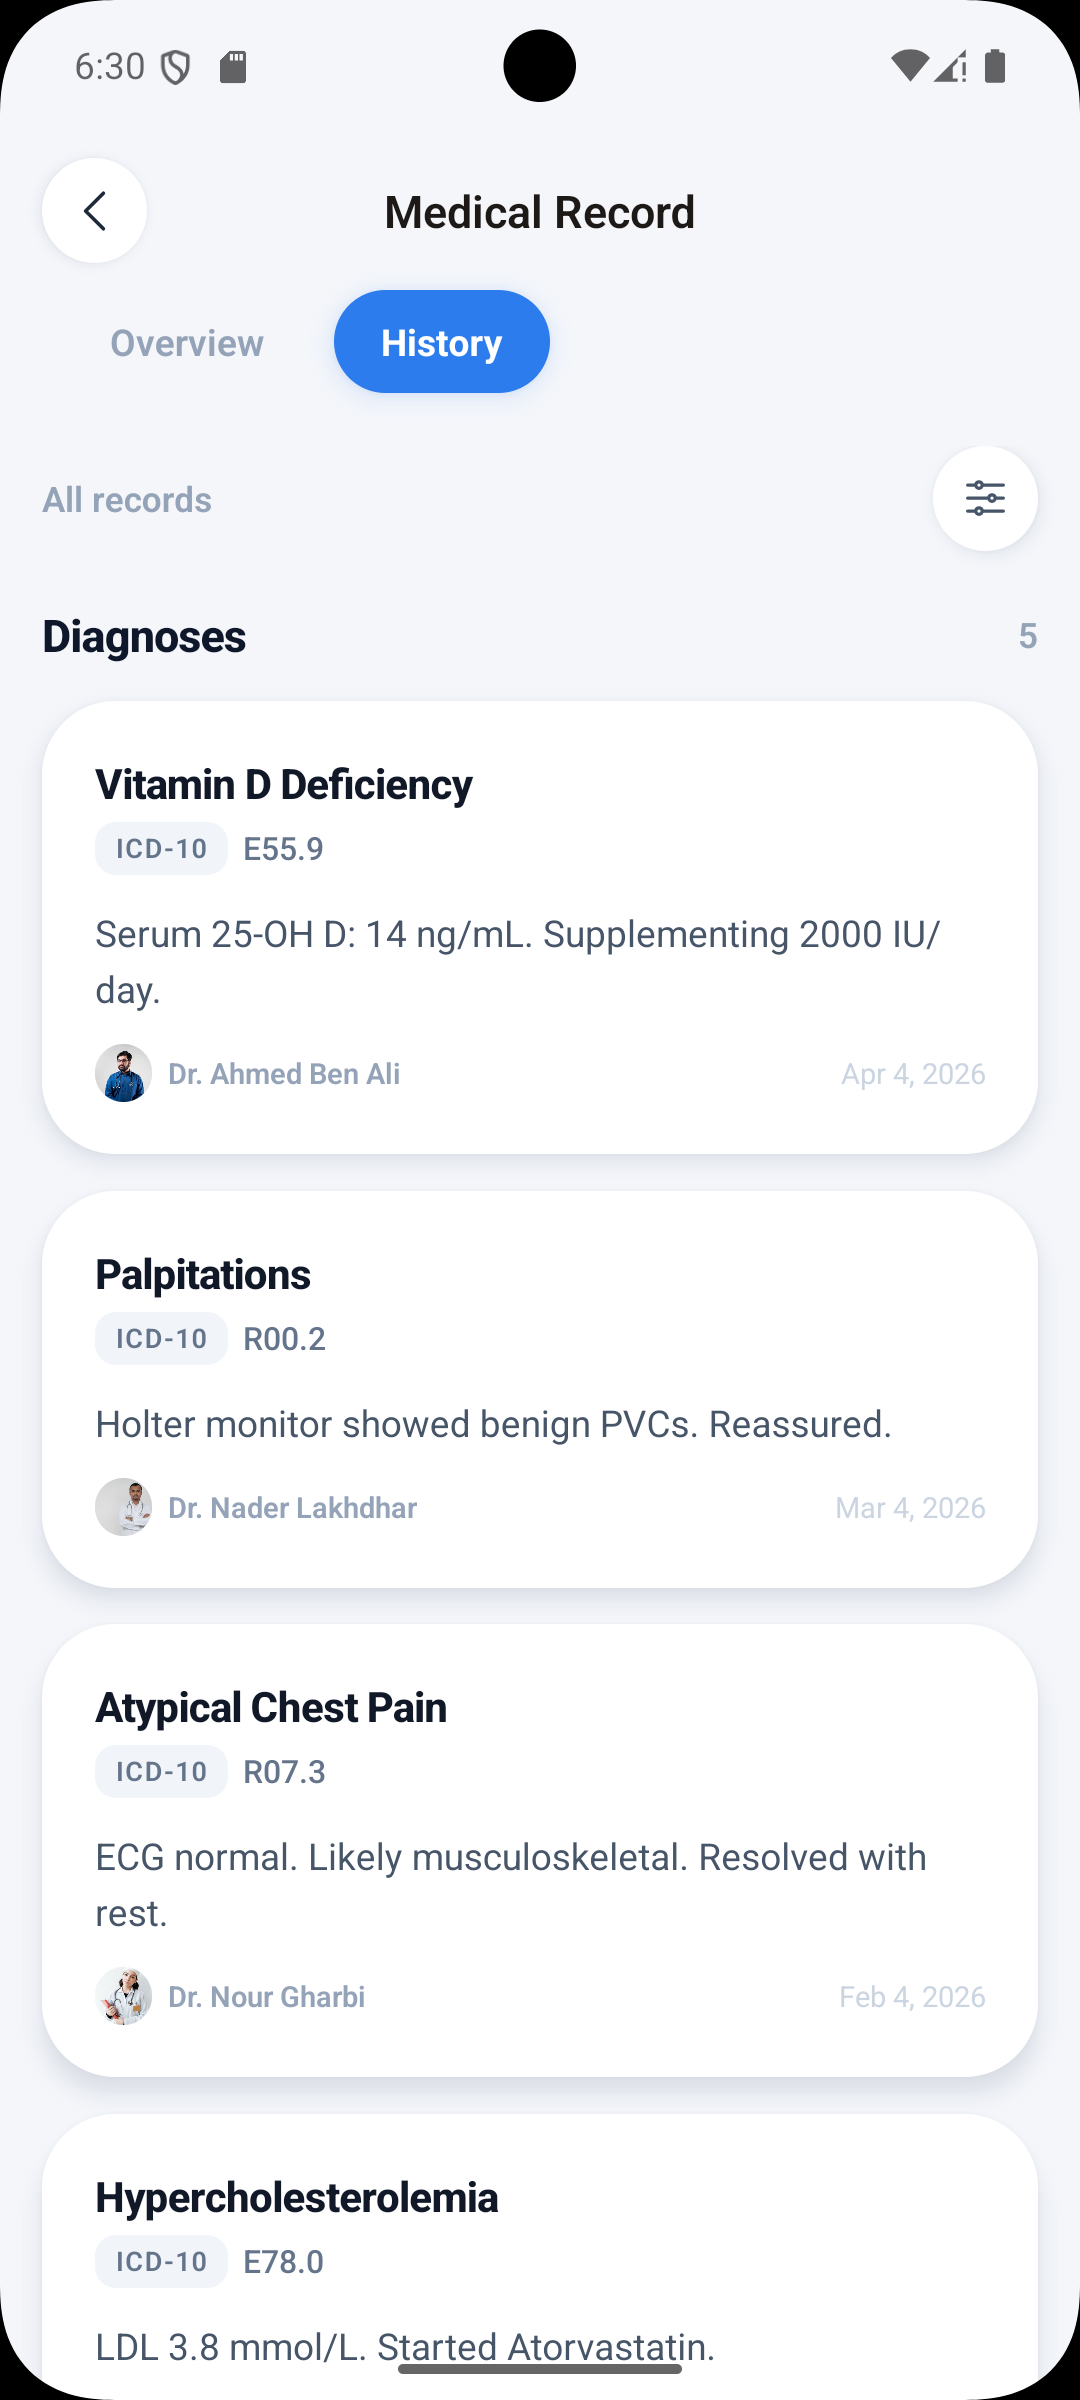
\includegraphics[width=\textwidth,height=0.70\textheight,keepaspectratio]{screen-medical-record2.png}
    \end{minipage}
    \caption{Patient Medical Record Interface}
    \label{fig:screen medical record}
\end{figure}

\subsection{Medication Management}

The medication dashboard presents the patient's active prescriptions with a \textbf{daily dose by dose tracking interface}. Each medication displays:

\begin{itemize}
    \item Medication name, dosage, frequency, and administration route.
    \item Time slot pills (morning, afternoon, evening, night) with status indicators.
    \item Action buttons to mark each dose as taken, missed, or skipped.
    \item An \textbf{adherence progress ring} showing the percentage of doses taken.
\end{itemize}

The \texttt{medication reminder cron} Edge Function runs every 15~minutes and sends push notifications via Firebase Cloud Messaging~\cite{fcm} for upcoming doses.

\begin{figure}[H]
    \centering
    \begin{minipage}{0.30\textwidth}
        \centering
        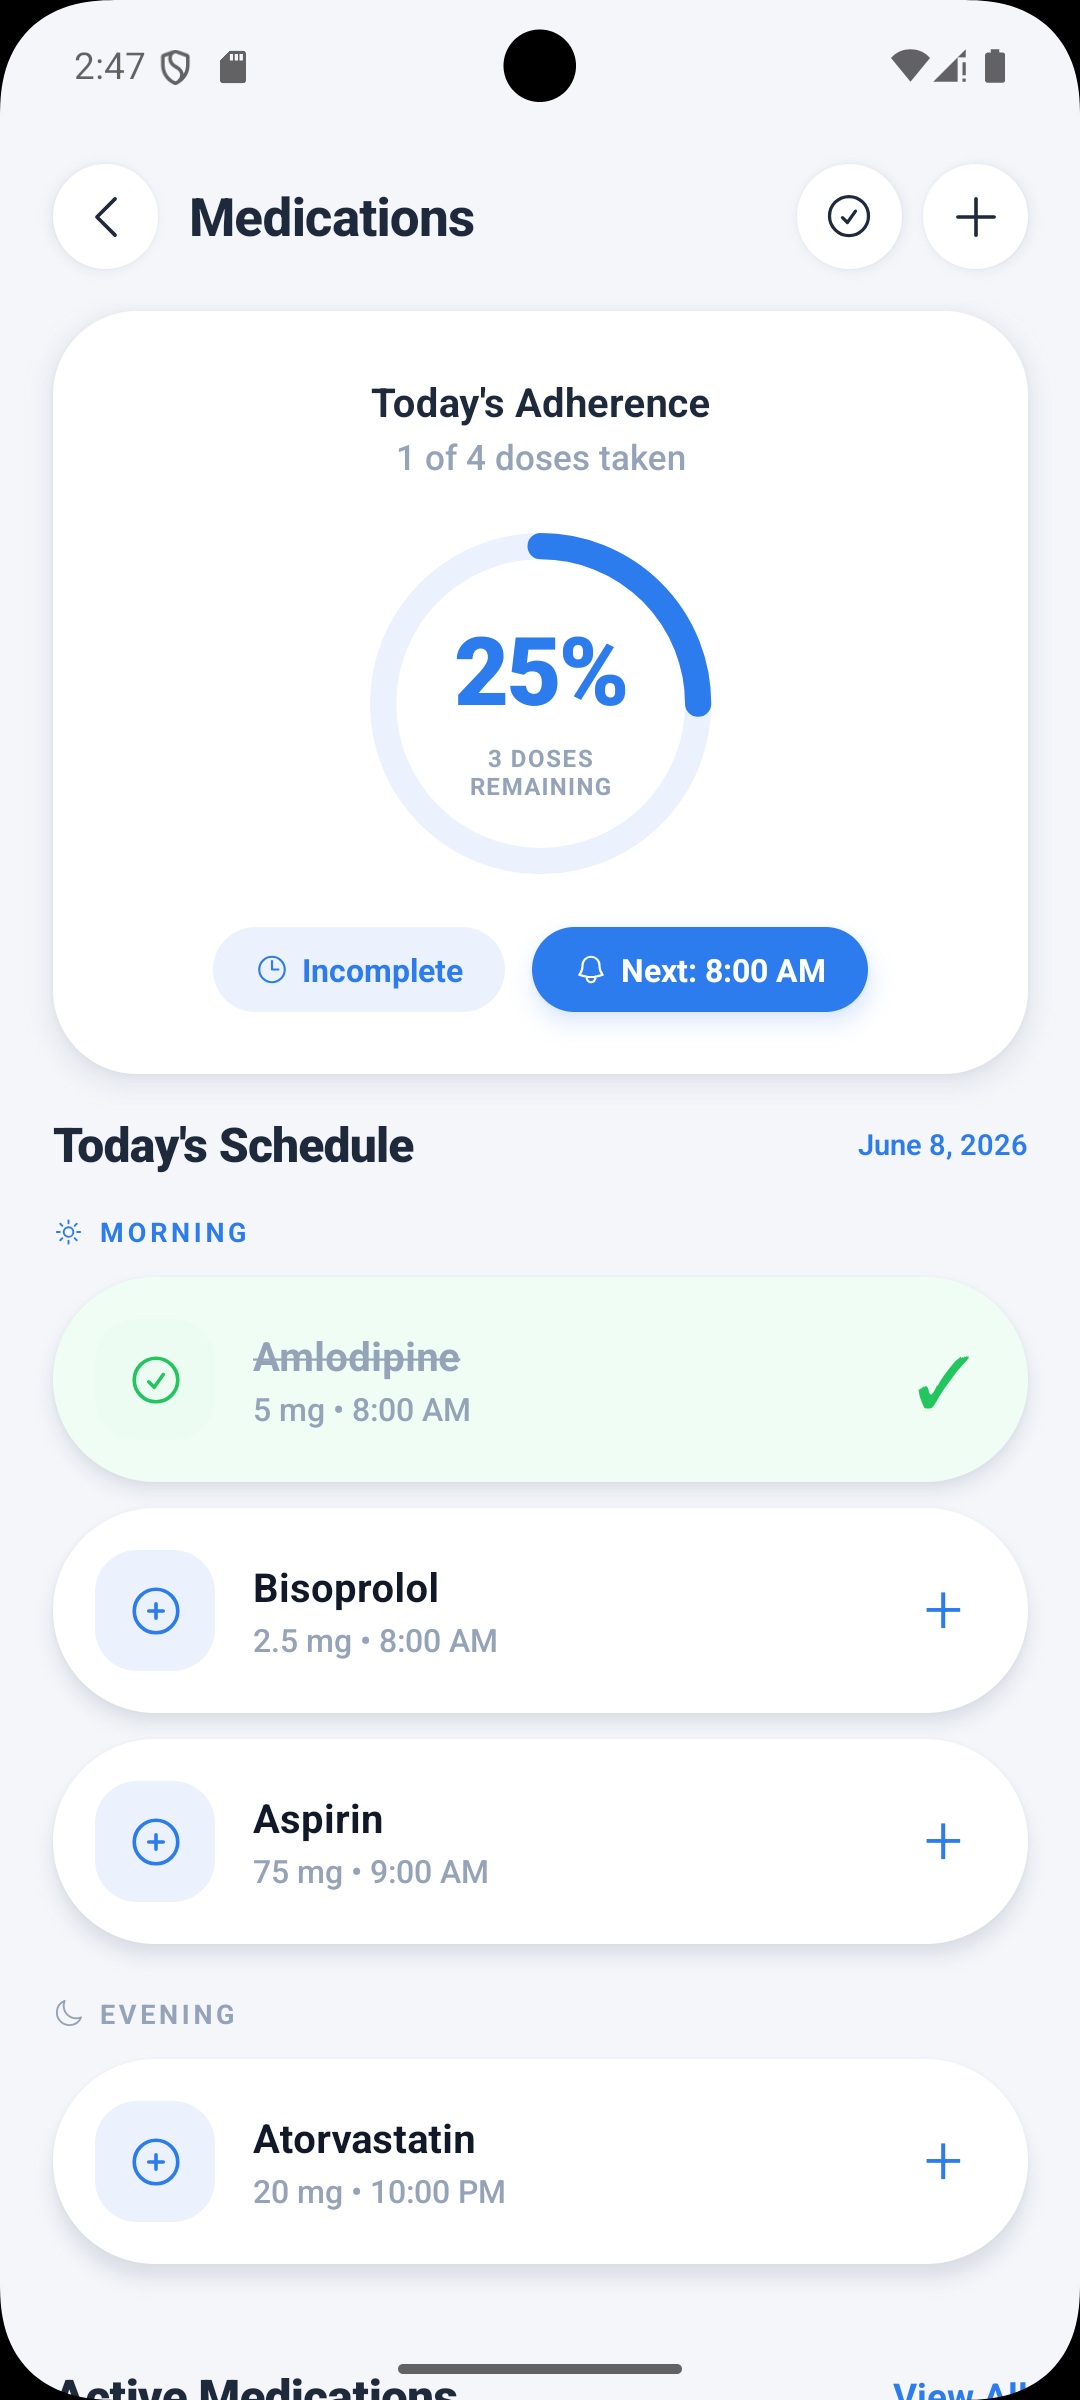
\includegraphics[width=\textwidth,height=0.70\textheight,keepaspectratio]{screen-medications.png}
    \end{minipage}\hfill
    \begin{minipage}{0.30\textwidth}
        \centering
        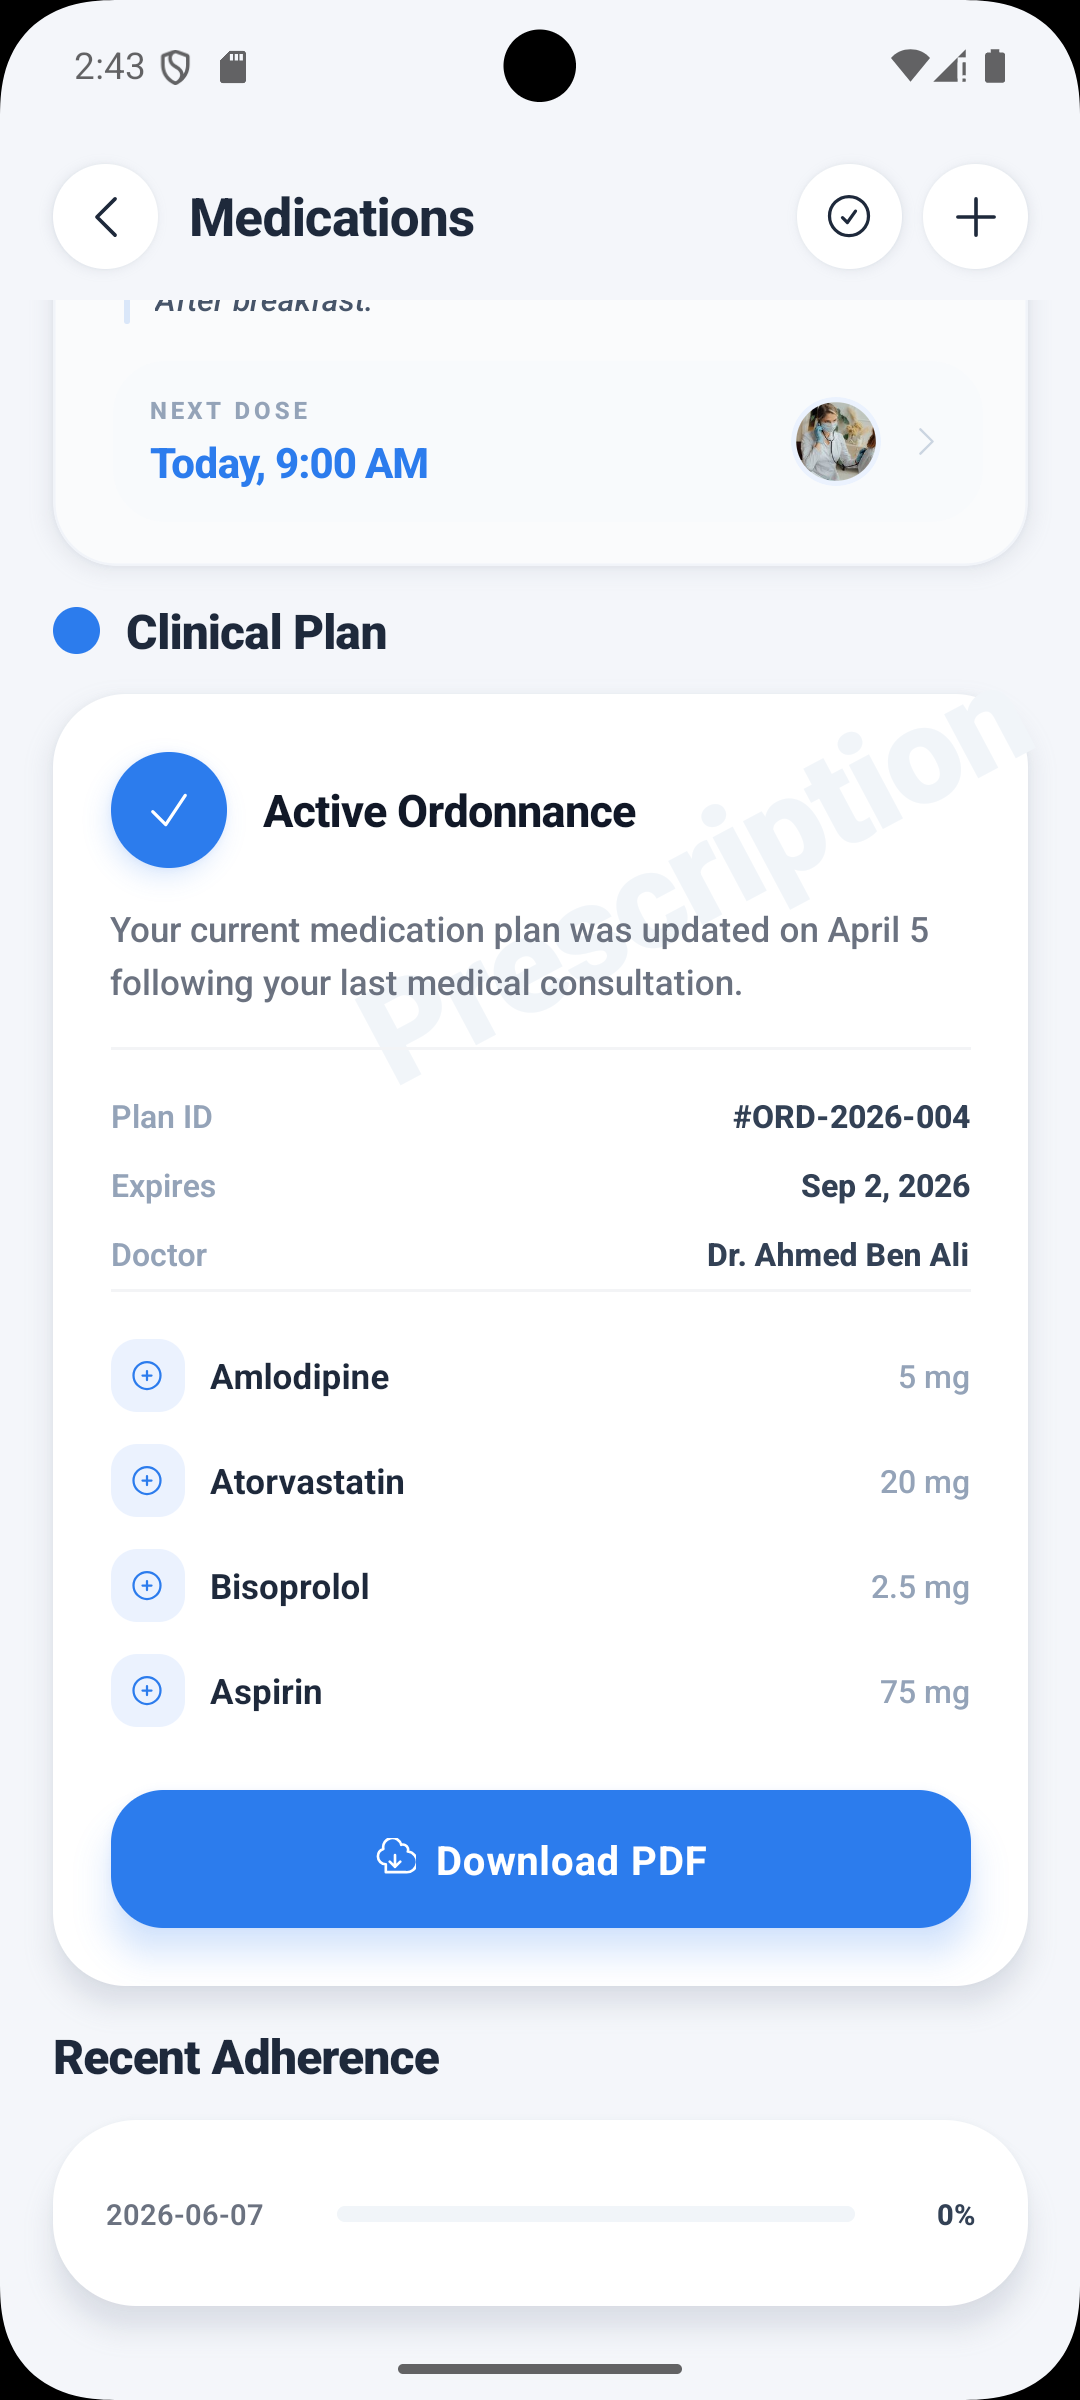
\includegraphics[width=\textwidth,height=0.70\textheight,keepaspectratio]{medidcation2.png}
    \end{minipage}\hfill
    \begin{minipage}{0.30\textwidth}
        \centering
        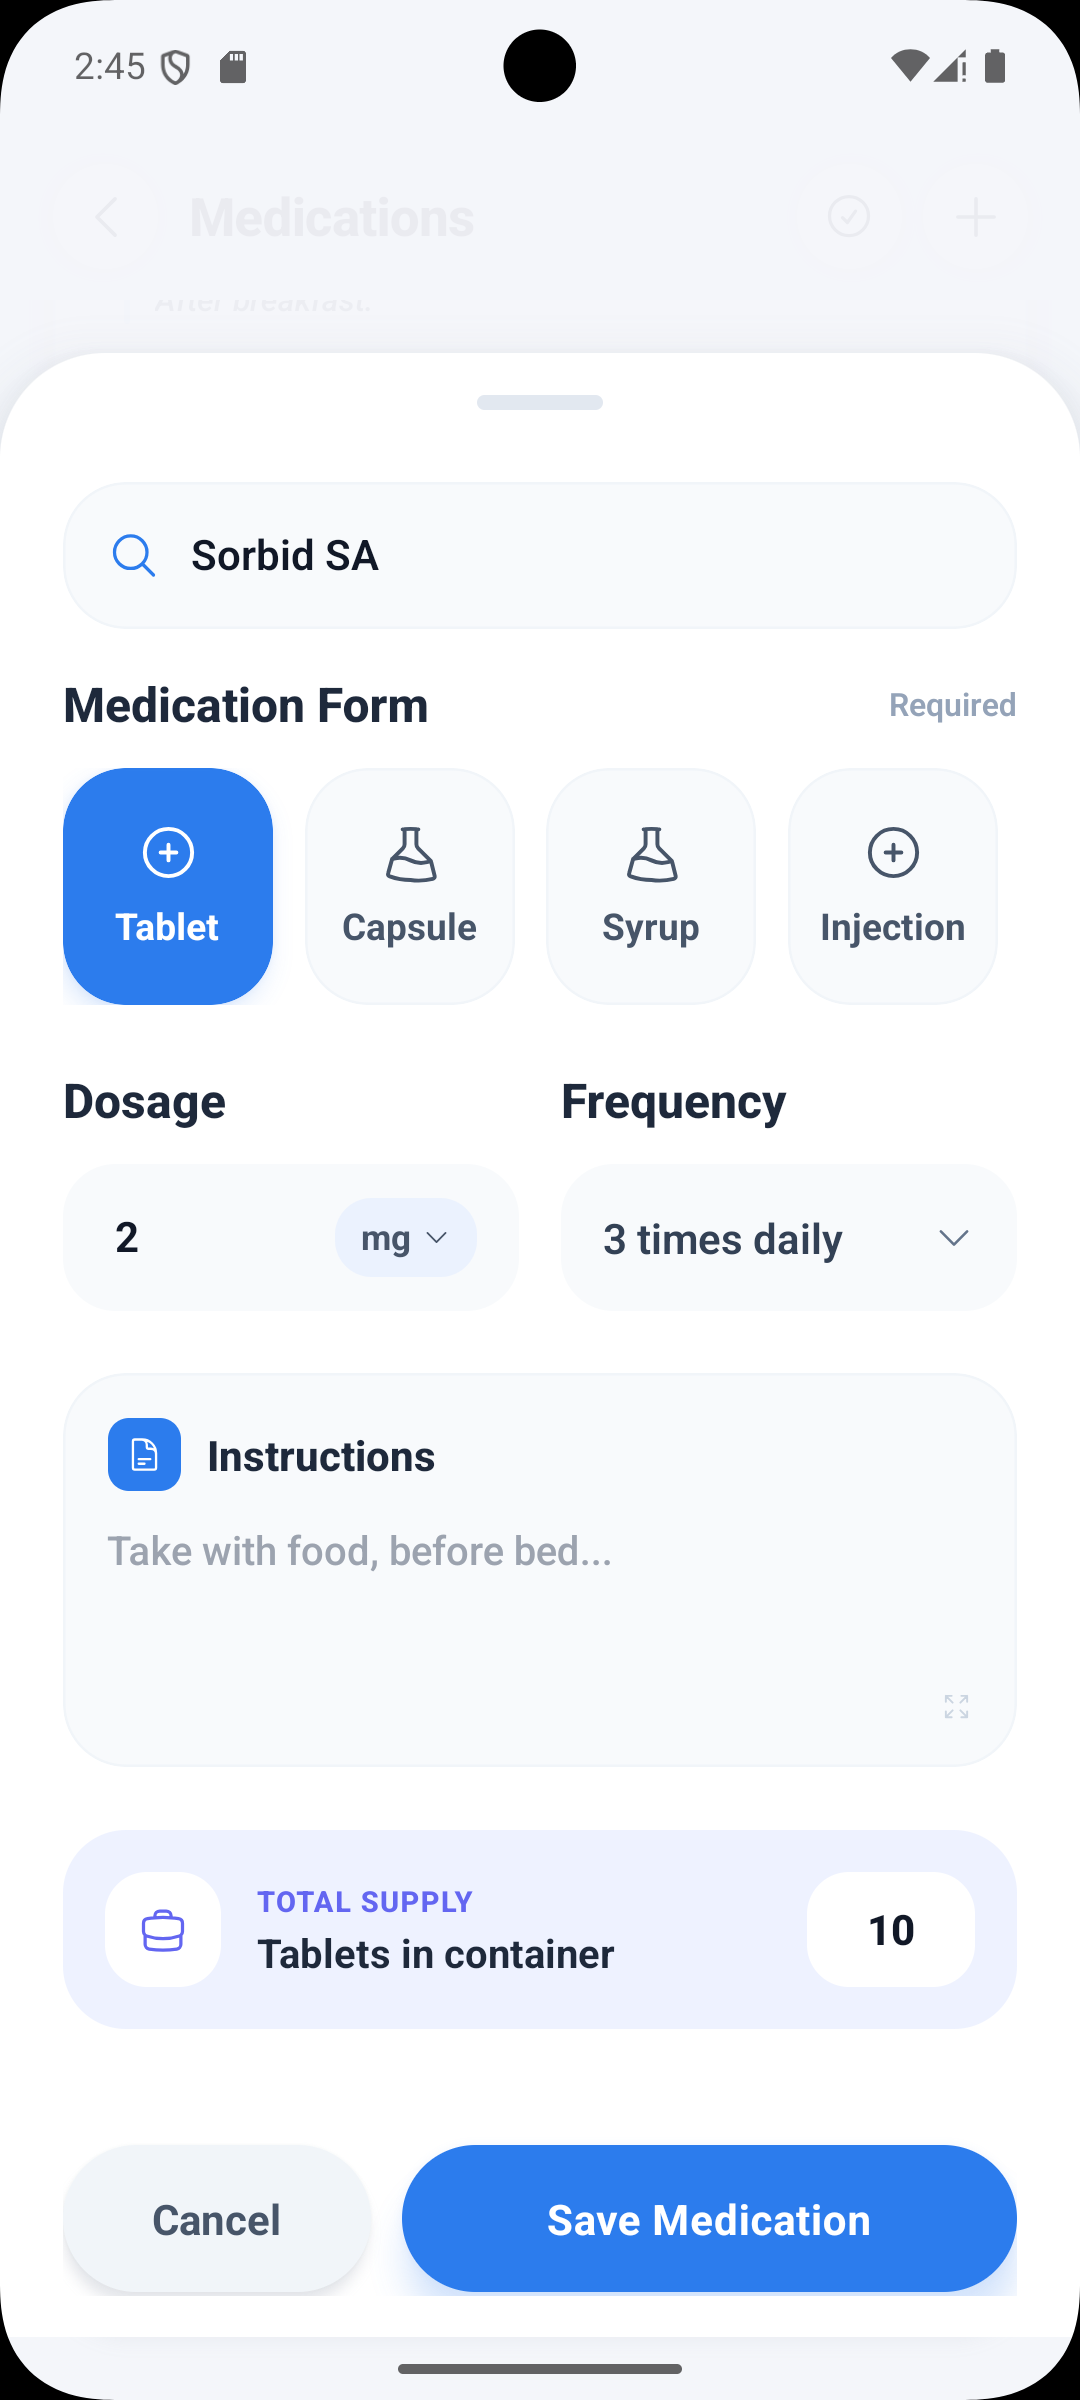
\includegraphics[width=\textwidth,height=0.70\textheight,keepaspectratio]{medication3.png}
    \end{minipage}
    \caption{Medication Management Dashboard}
    \label{fig:screen medications}
\end{figure}

\subsection{Laboratory Results and Trends}

The laboratory module allows patients to view their analysis results with:

\begin{itemize}
    \item Per biomarker values with reference ranges and abnormality flags (high, low, critical).
    \item \textbf{Trend charts} with cubic B\'ezier smoothing showing the evolution of key biomarkers
    \item Categorized views: hematology, lipid panel, metabolic, liver function, kidney function, endocrine, cardiac markers.
    \item \textbf{Lab report upload} with OCR parsing: the patient photographs a paper lab report, and the \texttt{parse lab upload} Edge Function (GPT 4o Vision) extracts all test values automatically.
\end{itemize}

\begin{figure}[H]
    \centering
    \begin{minipage}{0.45\textwidth}
        \centering
        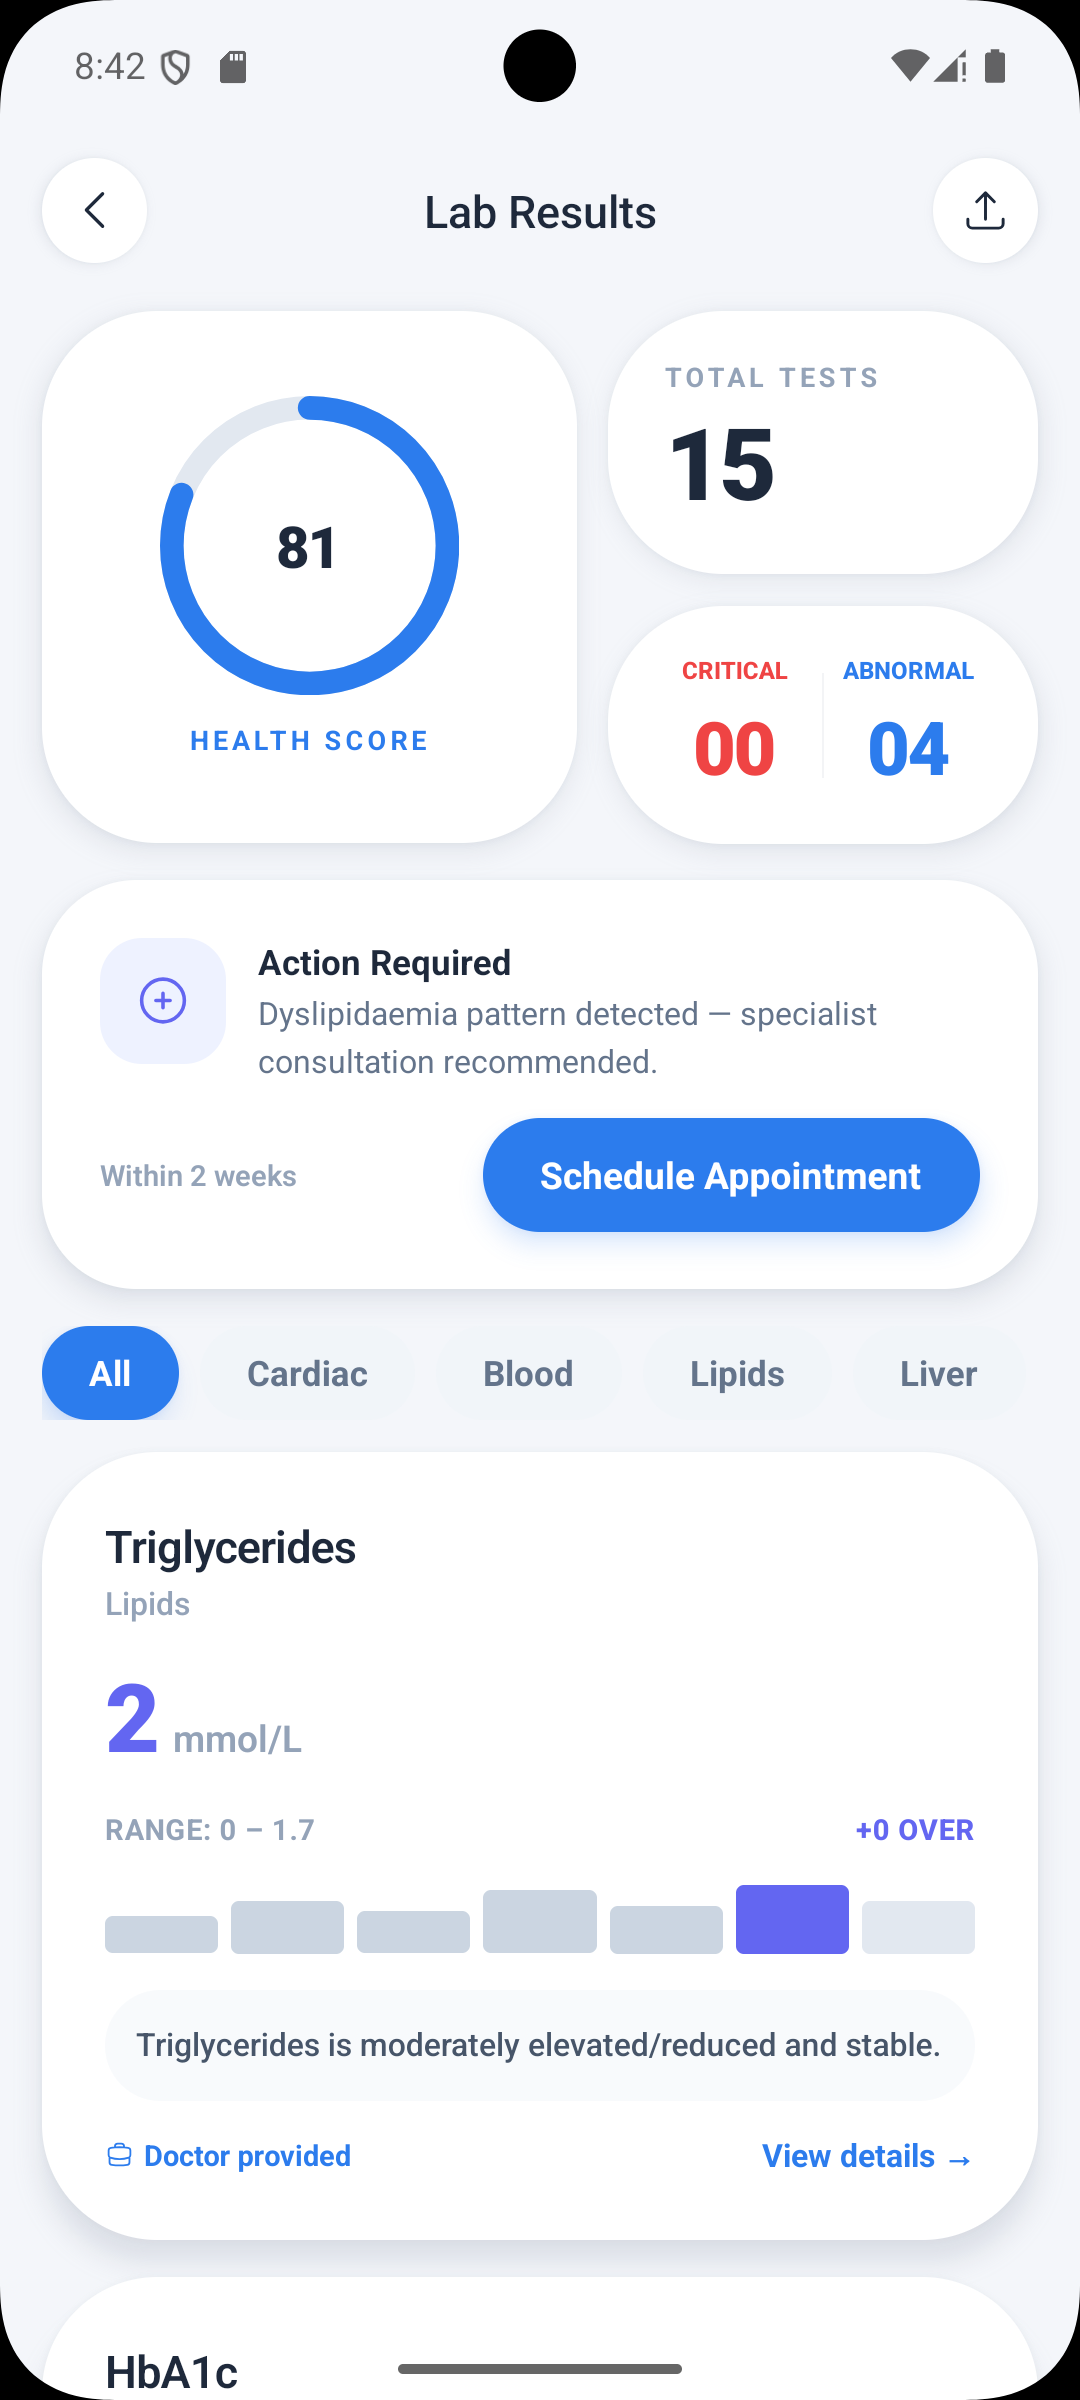
\includegraphics[width=\textwidth,height=0.58\textheight,keepaspectratio]{screen-lab-results.png}
    \end{minipage}\hfill
    \begin{minipage}{0.45\textwidth}
        \centering
        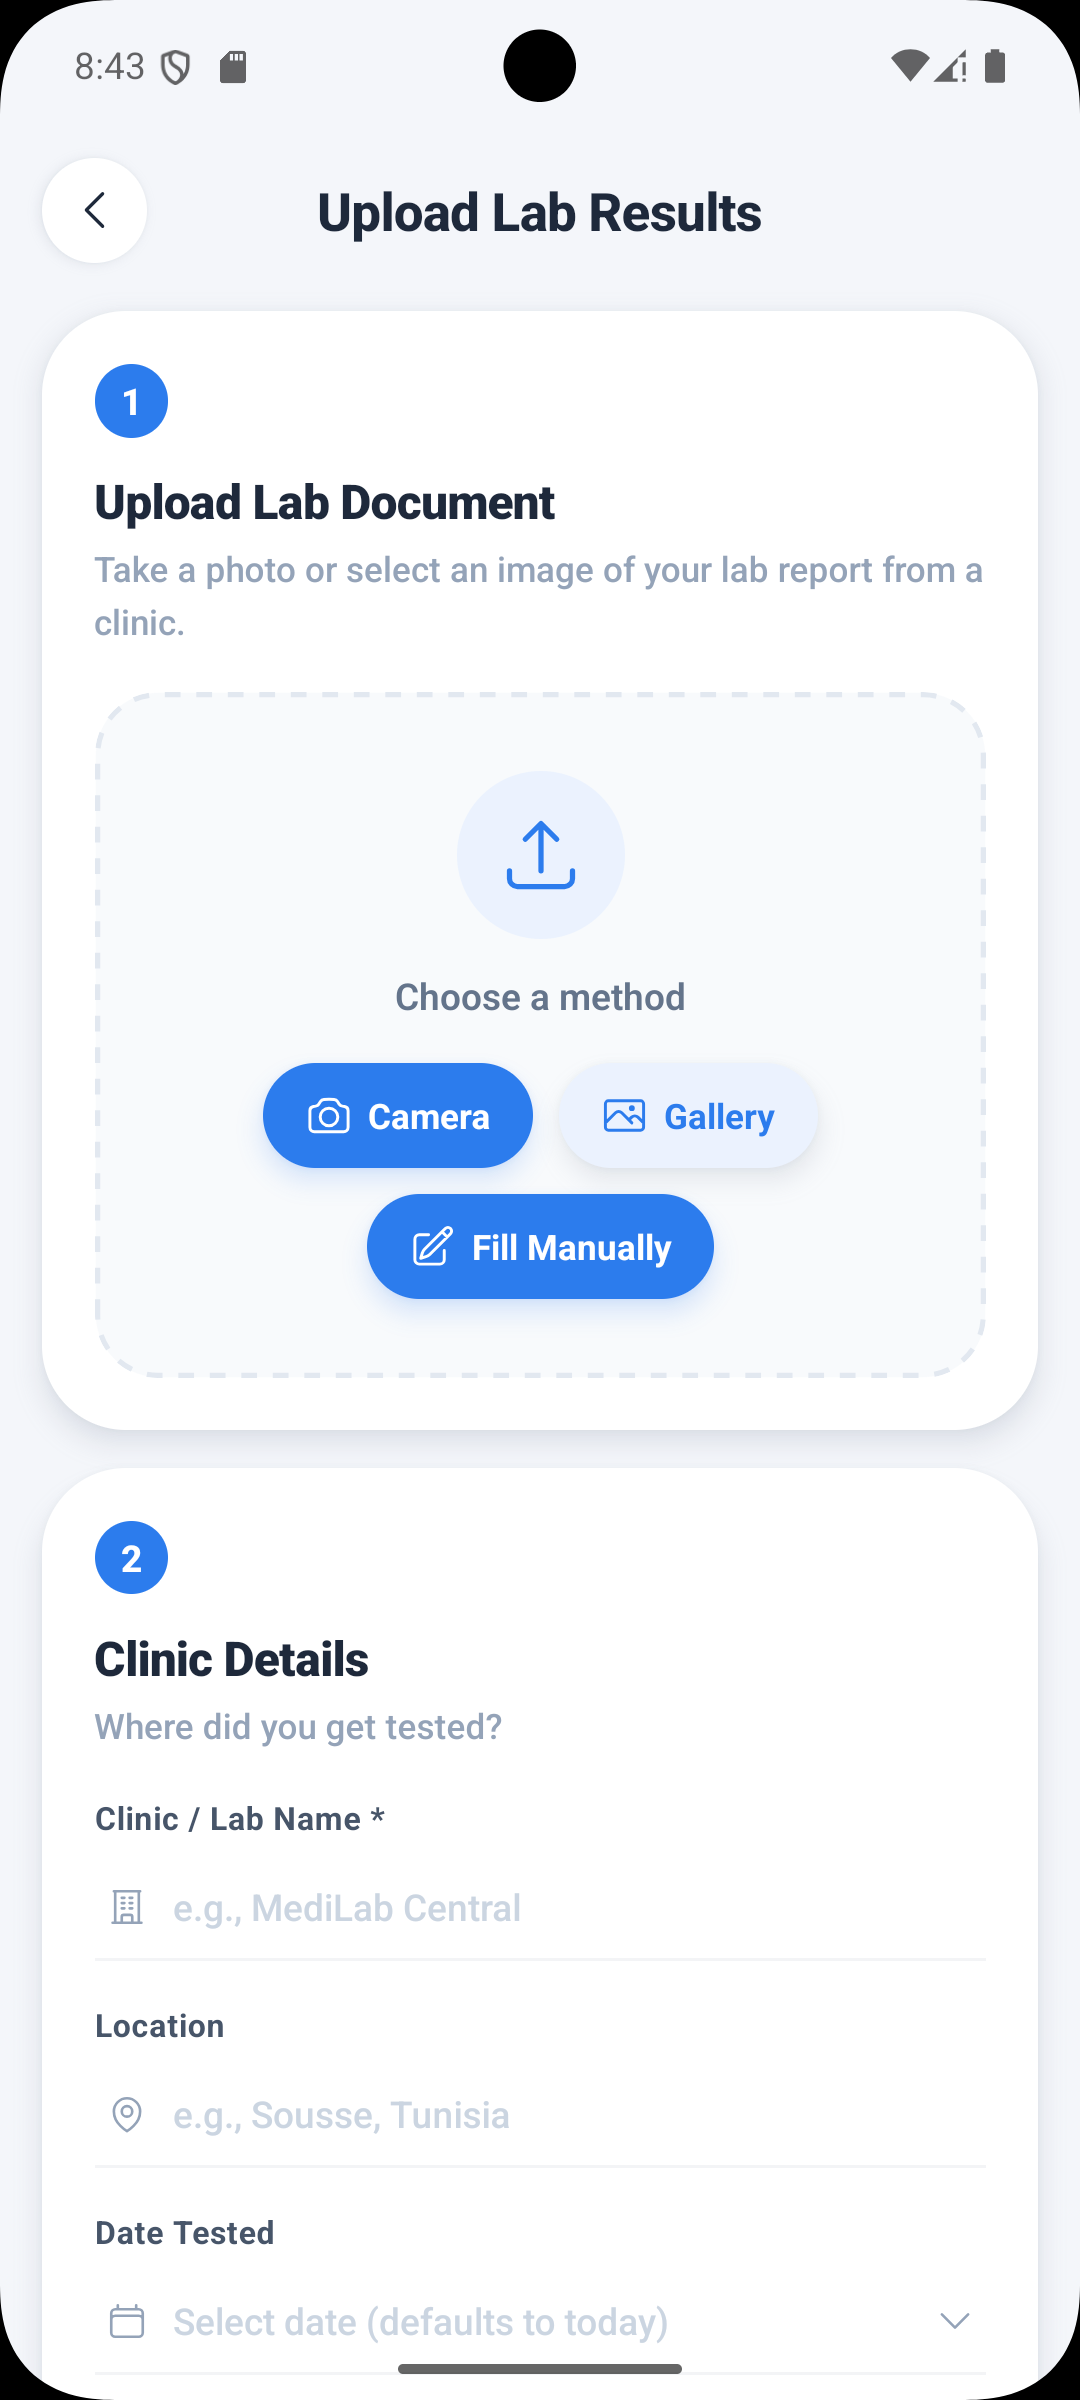
\includegraphics[width=\textwidth,height=0.58\textheight,keepaspectratio]{labresult2.png}
    \end{minipage}
    \caption{Laboratory Results with Trend Charts and OCR Upload}
    \label{fig:screen lab results}
\end{figure}

\subsection{Patient Recovery Index (PRI)}

The Recovery Index screen (Figure~\ref{fig:screen pri}) presents the Patient Recovery Index, a composite weighted score from 0 to 100 computed by the \texttt{compute pri} Edge Function. The interface features:

\begin{itemize}
    \item A central \textbf{progress ring} with animated score display.
    \item A \textbf{radar chart} (pentagon) visualizing five sub scores: symptoms, medication adherence, laboratory results, physical activity, and medical evaluation.
    \item A \textbf{7 day history} with interactive day pills and sparkline trend chart.
    \item \textbf{Recovery drivers} showing the contribution factors with progress bars.
\end{itemize}

\begin{figure}[H]
    \centering
    \begin{minipage}{0.42\textwidth}
        \centering
        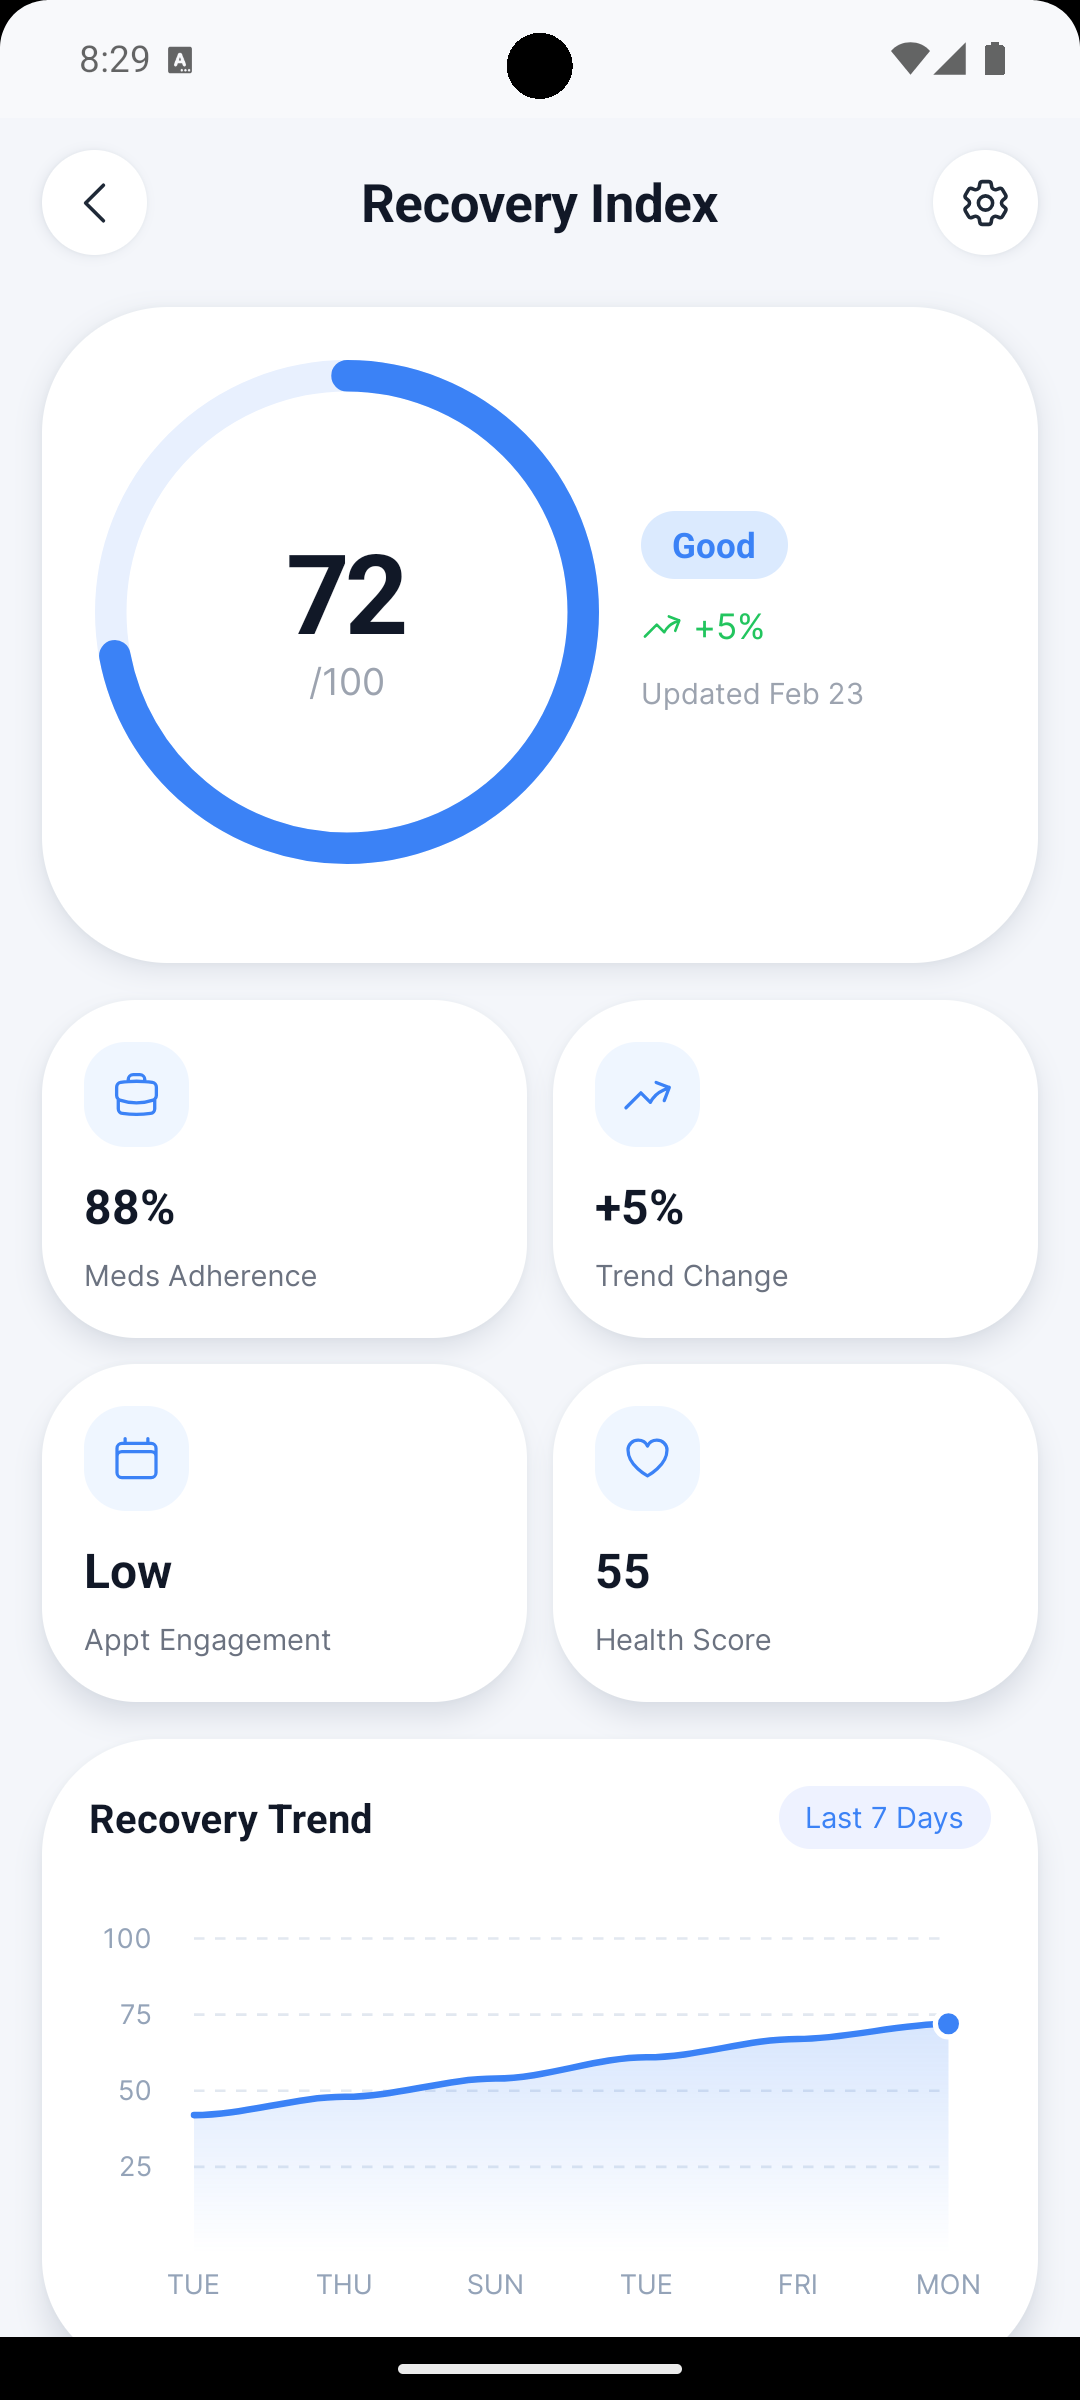
\includegraphics[width=\textwidth,height=0.70\textheight,keepaspectratio]{screen-recovery-index.png}
    \end{minipage}\hfill
    \begin{minipage}{0.42\textwidth}
        \centering
        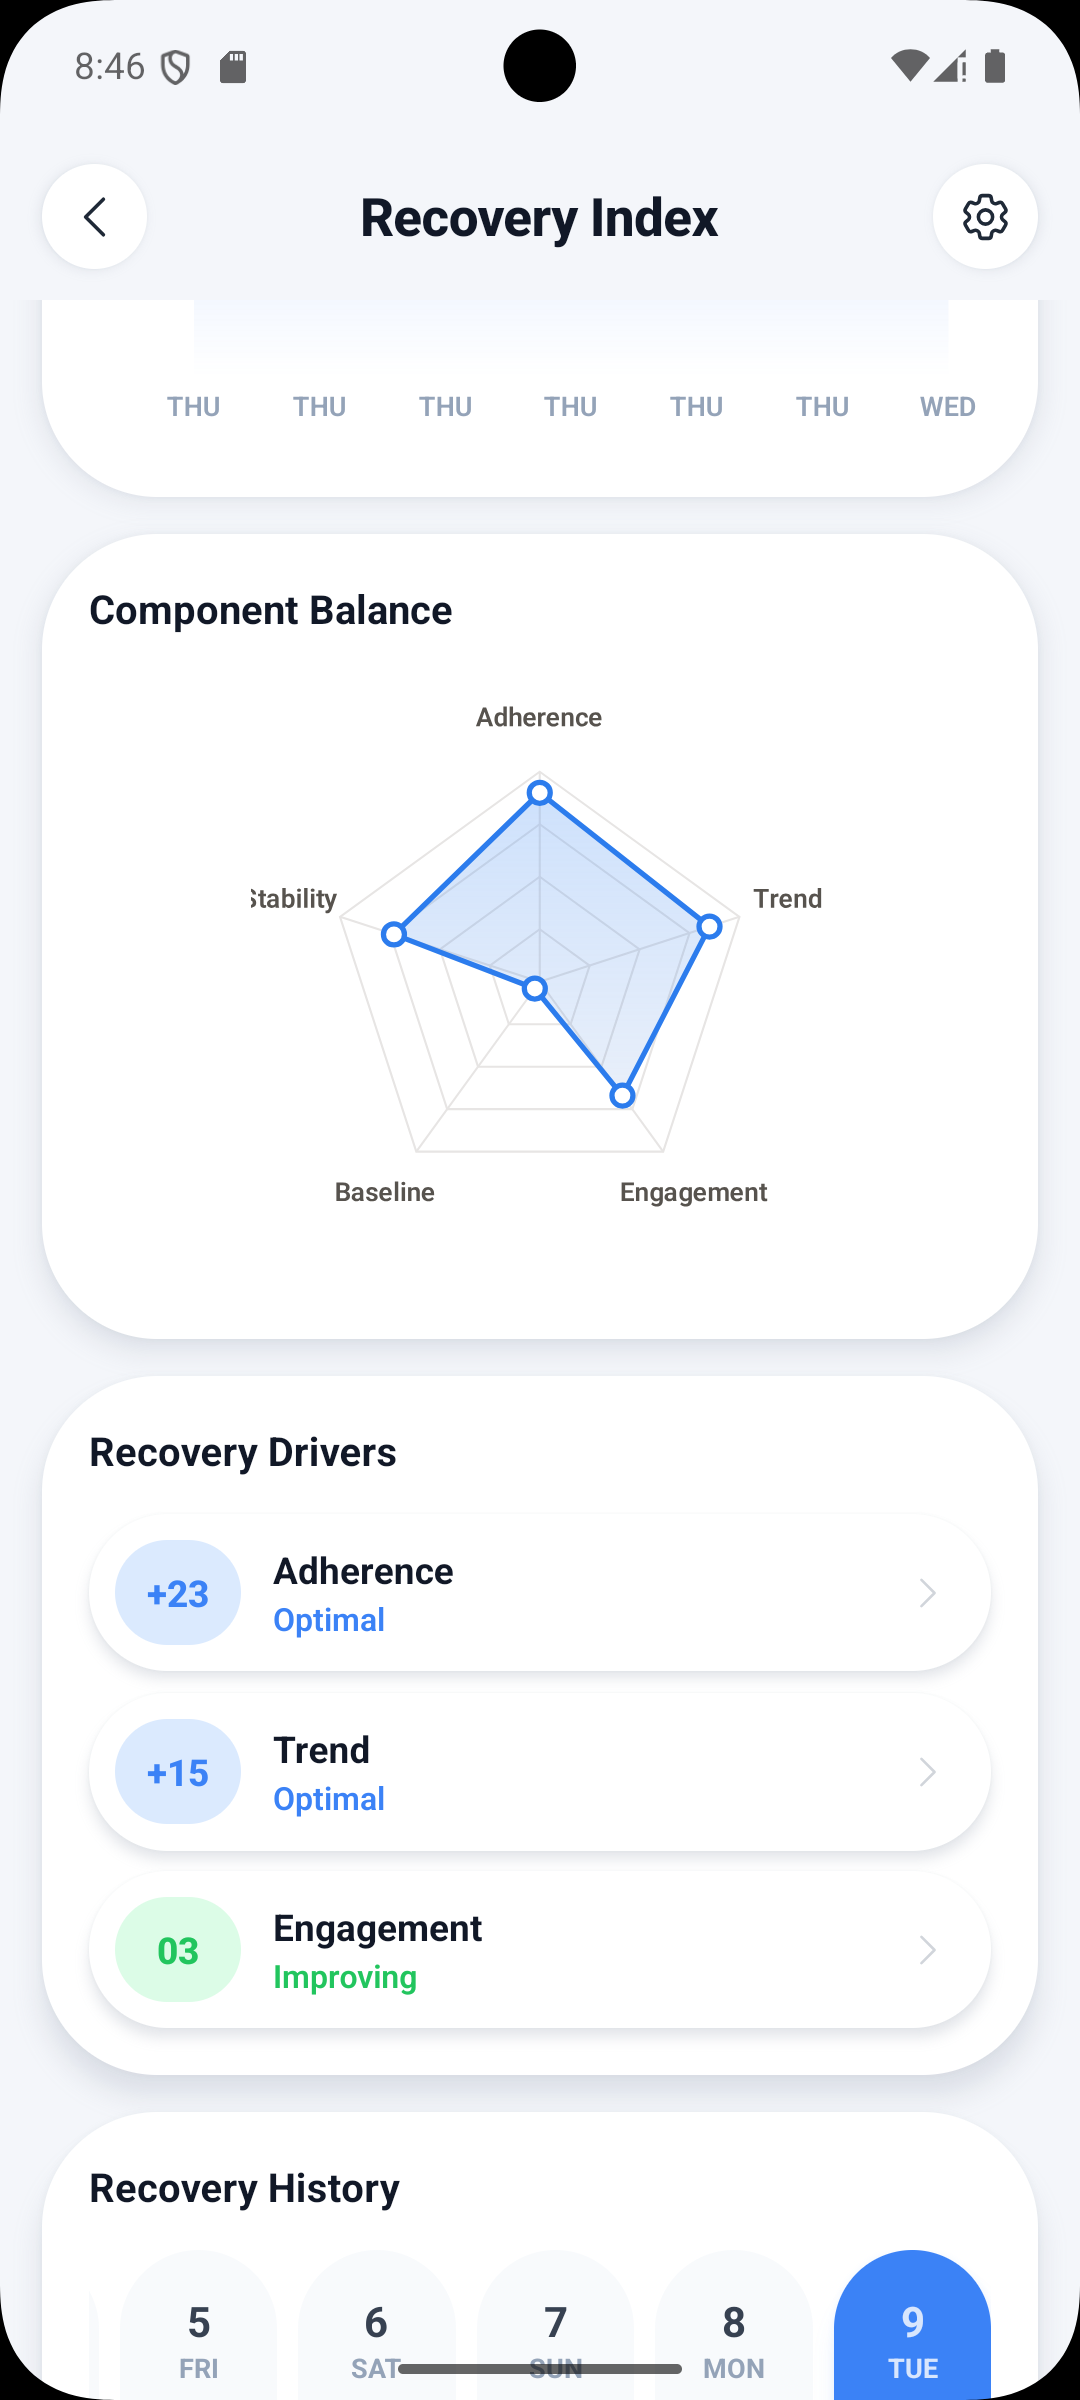
\includegraphics[width=\textwidth,height=0.70\textheight,keepaspectratio]{recoveryindex2.png}
    \end{minipage}
    \caption{Patient Recovery Index (PRI) Dashboard}
    \label{fig:screen pri}
\end{figure}

\subsection{Predictive Risk Assessment}

The predictive risk screen implements a \textbf{hybrid local then AI approach}: risk scores are first computed locally via \texttt{localRiskCalculator.ts} for instant display, then refined by the \texttt{predictHealthRisks} AI function in the background. The interface features:

\begin{itemize}
    \item A \textbf{semi gauge} with animated arc showing the overall risk score.
    \item \textbf{Category cards} for cardiovascular risk, diabetes risk, hospitalization risk, and medication non adherence risk.
    \item Color coded thresholds: green ($\leq$25), amber (26 to 50), indigo (51 to 75), red ($>$75).
    \item \textbf{Risk drivers} ranked by impact with actionable recommendations.
    \item A \textbf{data completeness indicator} showing what information is missing for more accurate predictions.
\end{itemize}

\begin{figure}[H]
    \centering
    \begin{minipage}{0.42\textwidth}
        \centering
        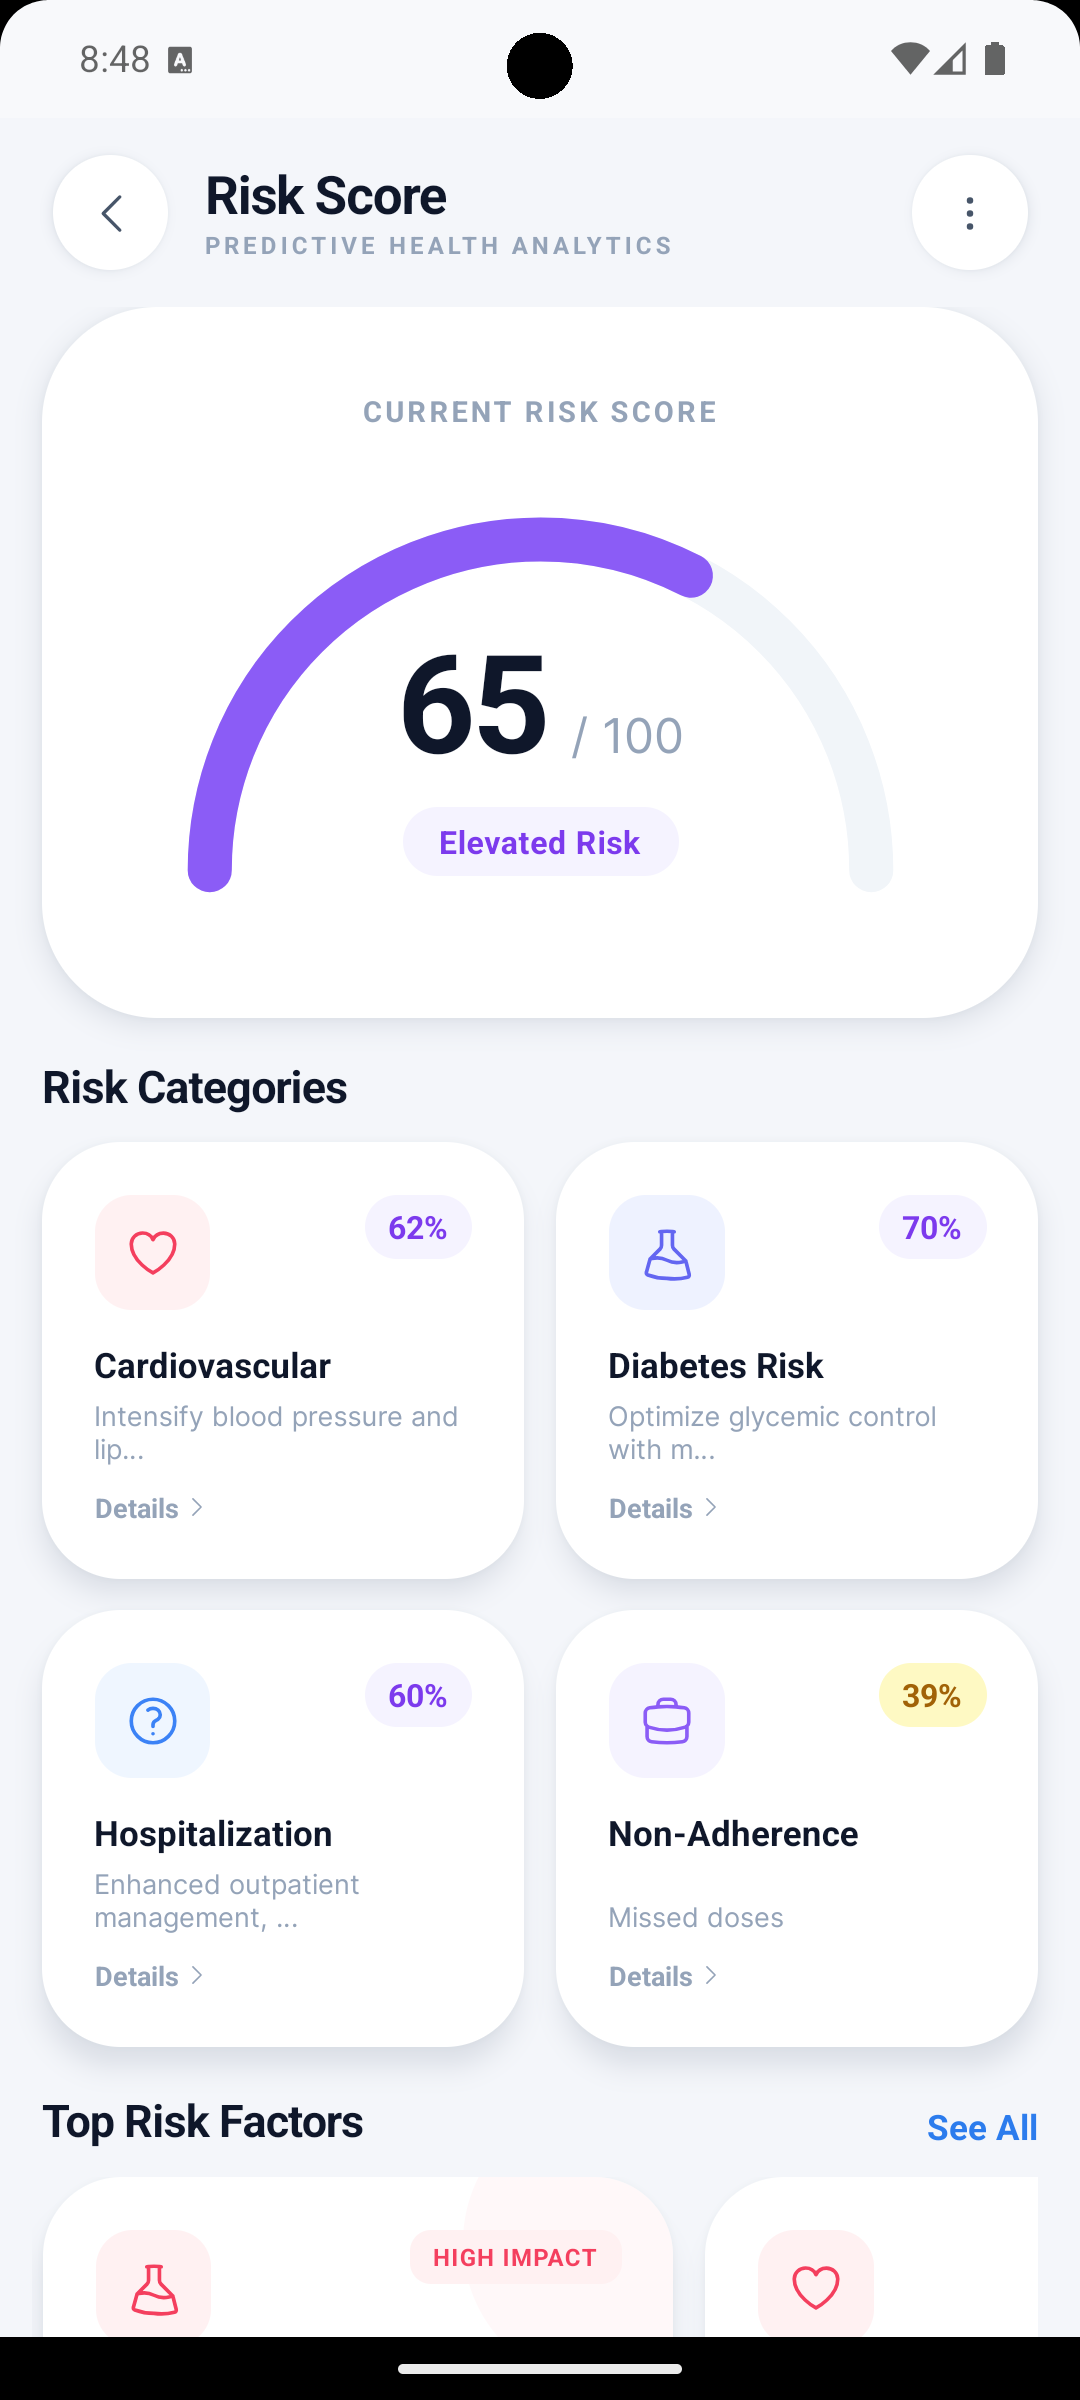
\includegraphics[width=\textwidth,height=0.70\textheight,keepaspectratio]{screen-predictive-risk.png}
    \end{minipage}\hfill
    \begin{minipage}{0.42\textwidth}
        \centering
        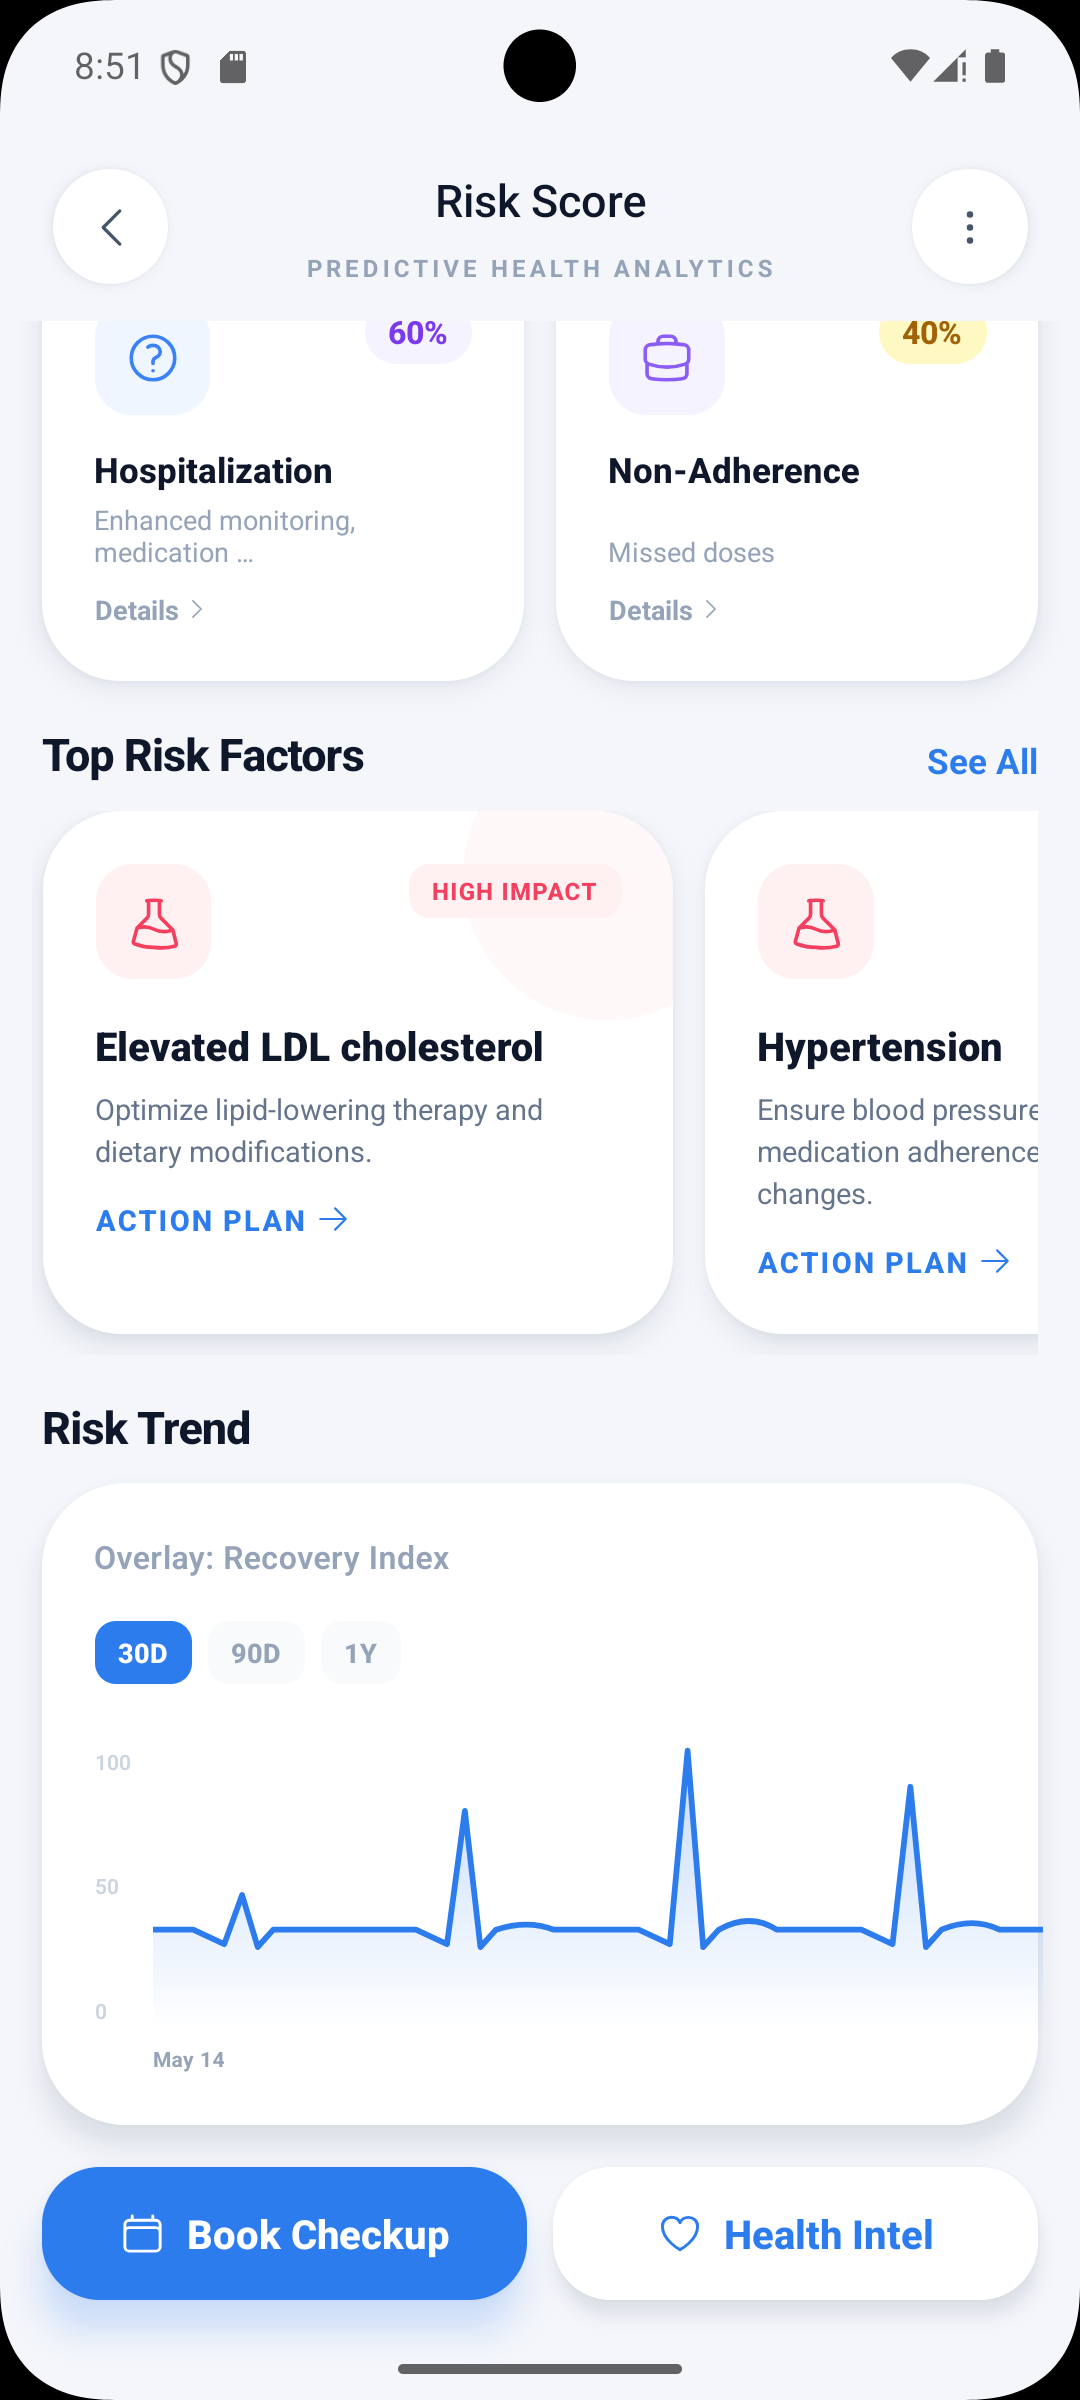
\includegraphics[width=\textwidth,height=0.70\textheight,keepaspectratio]{riskscore2.png}
    \end{minipage}
    \caption{Predictive Risk Assessment with Semi Gauge}
    \label{fig:screen predictive risk}
\end{figure}

\subsection{Sleep Quality Monitoring}

The sleep module provides a comprehensive sleep tracking experience:

\begin{itemize}
    \item \textbf{Sleep onboarding} to establish baseline sleep preferences.
    \item \textbf{Active sleep tracking} with start/stop controls and duration timer.
    \item \textbf{Sleep Quality Index (SQI)} computed by the \texttt{compute sqi} Edge Function, with weighted components: Duration (35\%), Consistency (25\%), Night Interruptions (20\%), Sleep Disturbances (20\%).
    \item \textbf{Sleep stages visualization} with colored bars (deep, light, REM, awake).
    \item \textbf{Wake interruption analysis} with cause identification.
    \item \textbf{Sleep history} with weekly trend pills.
\end{itemize}

\begin{figure}[H]
    \centering
    \begin{minipage}{0.42\textwidth}
        \centering
        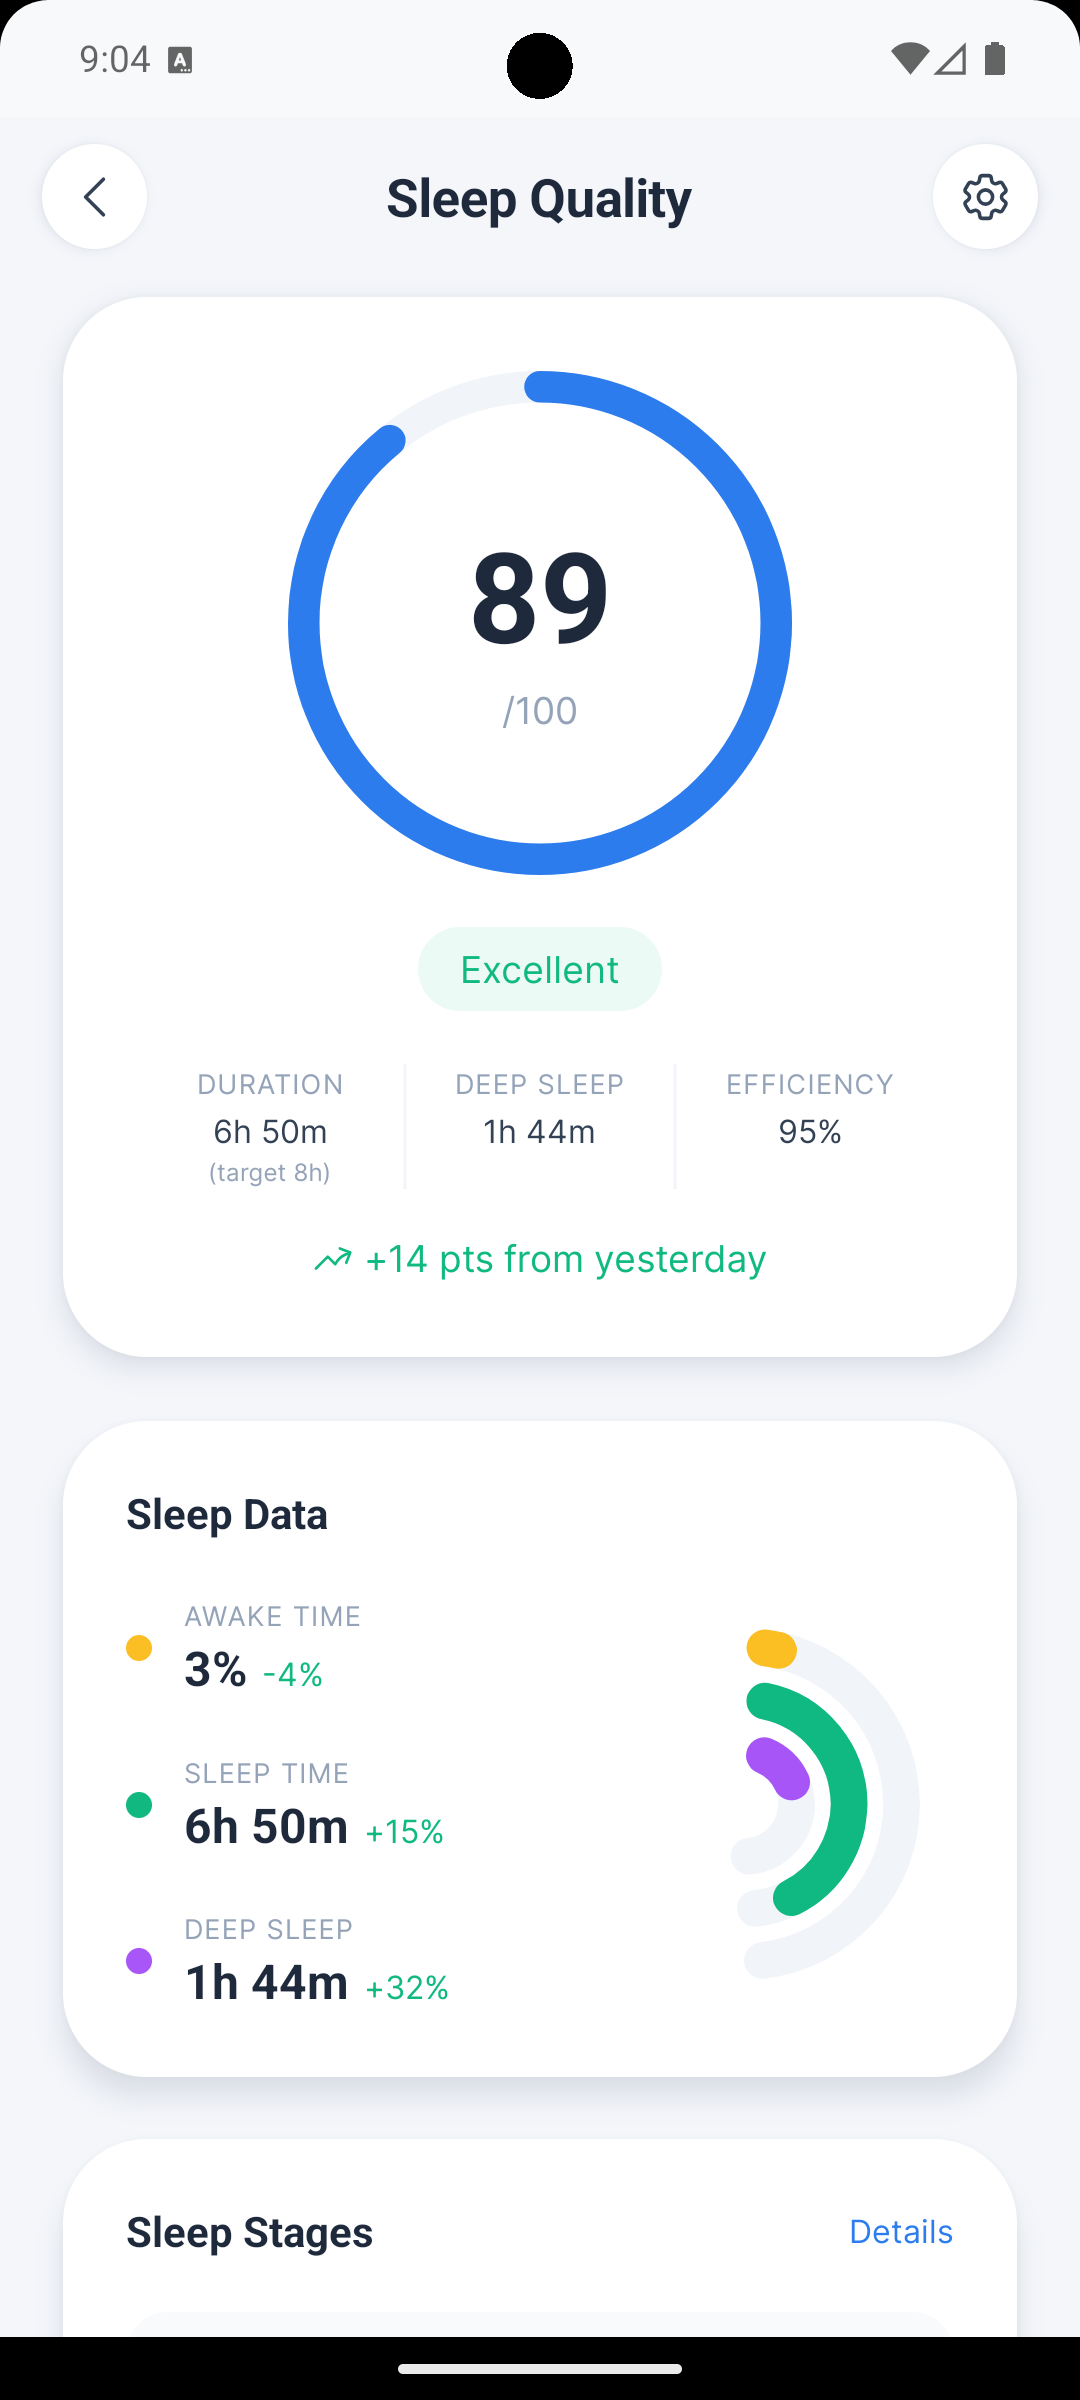
\includegraphics[width=\textwidth,height=0.70\textheight,keepaspectratio]{screen-sleep.png}
    \end{minipage}\hfill
    \begin{minipage}{0.42\textwidth}
        \centering
        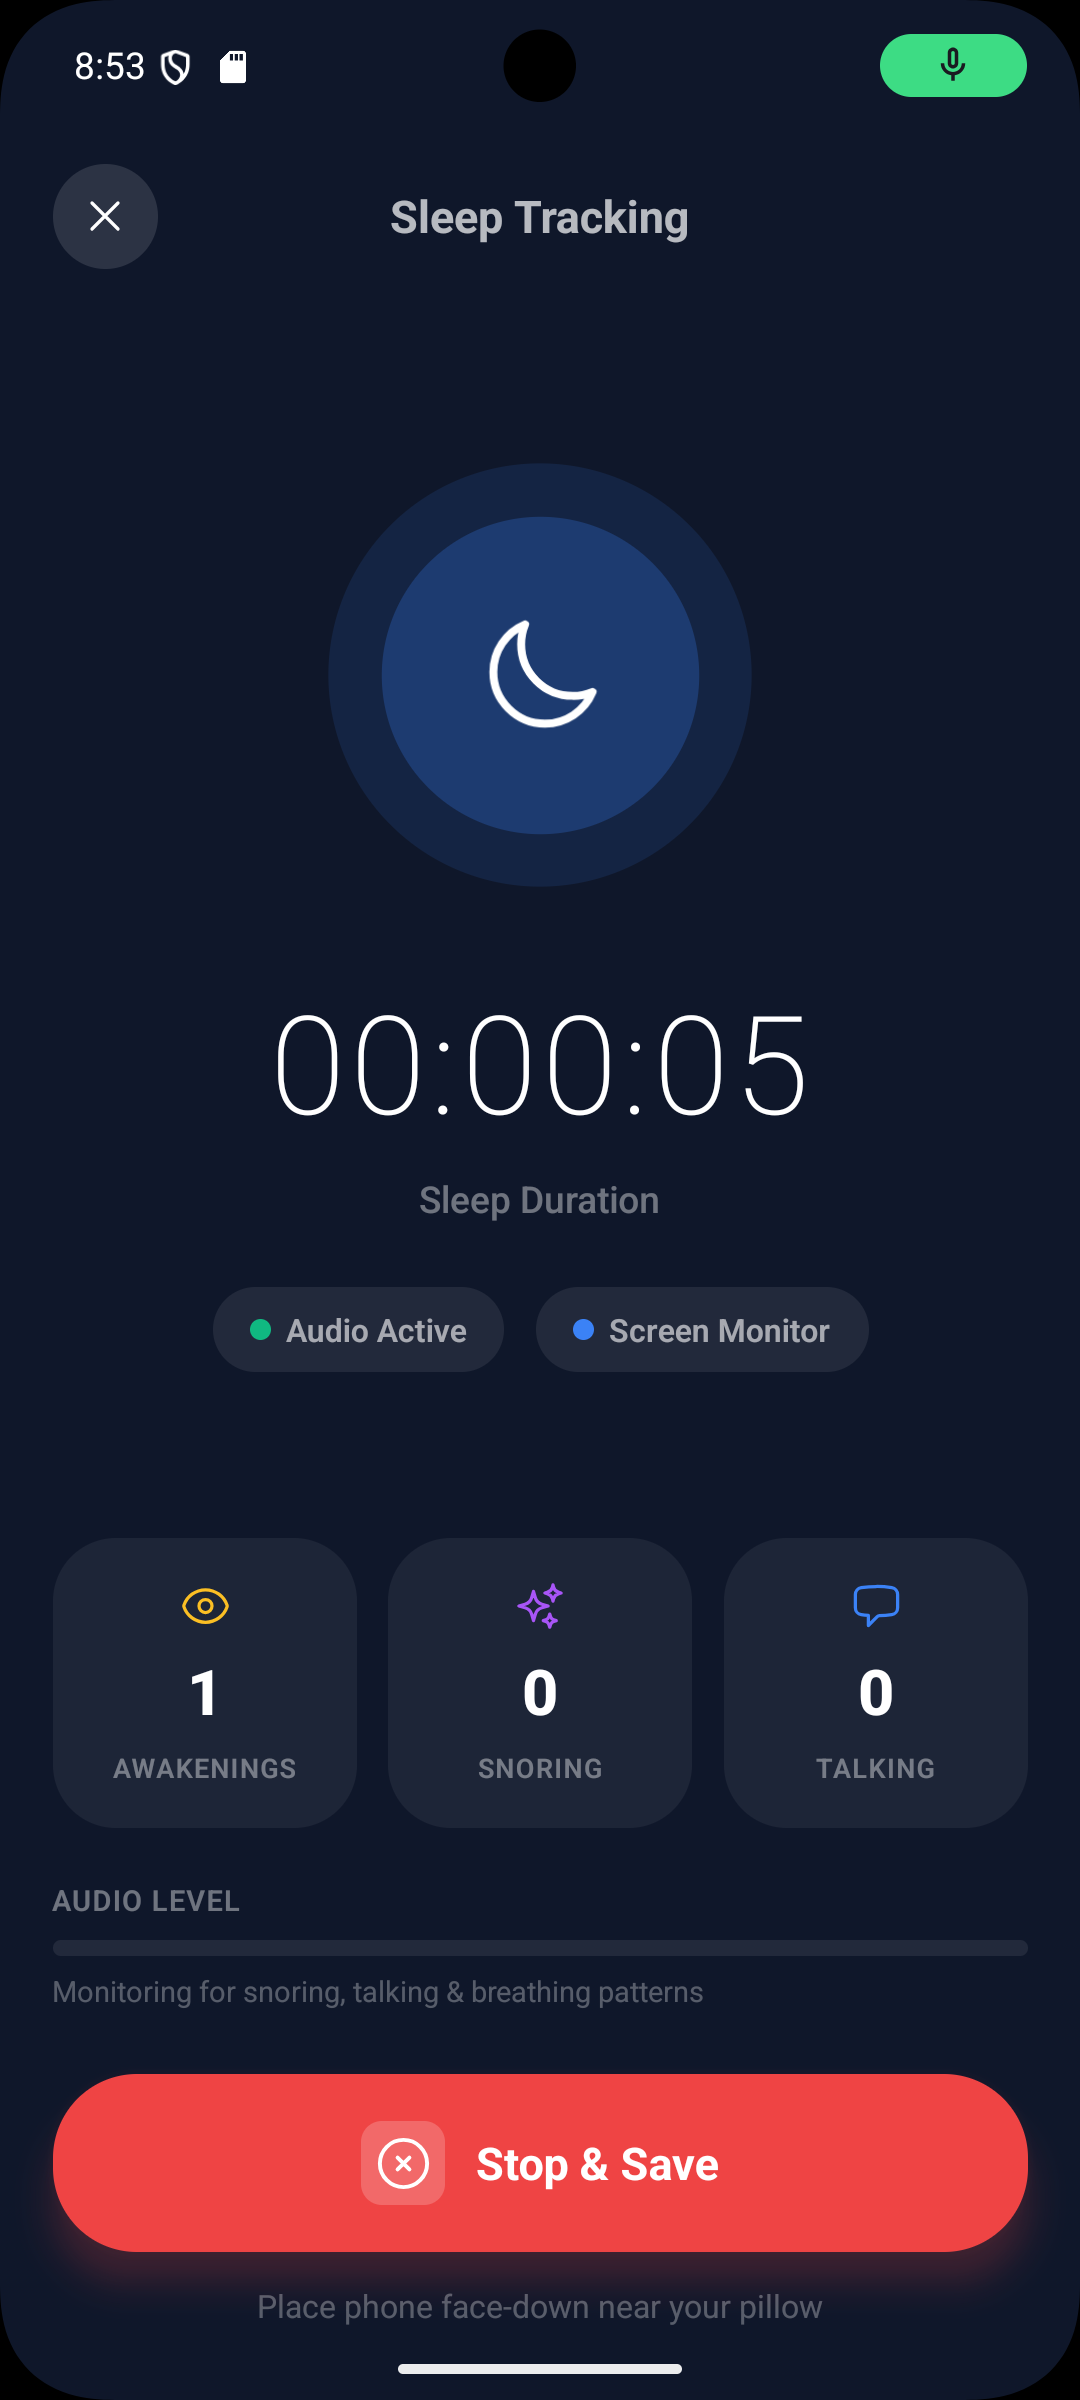
\includegraphics[width=\textwidth,height=0.70\textheight,keepaspectratio]{sleepquality2.png}
    \end{minipage}
    \caption{Sleep Quality Monitoring Dashboard}
    \label{fig:screen sleep}
\end{figure}

\subsection{Behavioral Health Tracking}

The behavioral health module enables longitudinal tracking of mental health indicators:

\begin{itemize}
    \item Daily mood, anxiety, sleep quality, stress level, and energy inputs.
    \item AI powered analysis (\texttt{analyzeBehavioralHealth}) producing a wellness score, stress index, burnout risk assessment, and CBT micro prompts.
    \item Trend visualization showing mood and stress evolution over time.
    \item Habit correlation analysis linking behavioral patterns to health outcomes.
\end{itemize}

\subsection{Emergency Mode}

The emergency screen provides a critical SOS feature:

\begin{itemize}
    \item A \textbf{countdown timer} (default 10 seconds) before automatically calling emergency services.
    \item \textbf{GPS geolocation} with real time coordinates.
    \item An \textbf{interactive Leaflet map}~\cite{leaflet} showing nearby hospitals, clinics, and pharmacies (via Overpass API with multi endpoint fallback and Nominatim backup).
    \item \textbf{Route planning} to the nearest facility (OSRM driving and walking directions).
    \item \textbf{Emergency notification} dispatched to the patient's treating physician and all platform administrators via the \texttt{emergency alert} Edge Function.
    \item \textbf{Medical snapshot sharing} critical medical data (allergies, chronic diseases, blood type, current medications) displayed for first responders.
\end{itemize}

\subsection{Real Time Messaging}

The messaging system enables bidirectional real time communication between patients and doctors:

\begin{itemize}
    \item Text messages, image sharing, and file attachments.
    \item Online presence indicators (green dot for active users).
    \item Typing indicators and read receipts.
    \item Push notifications for new messages via Firebase Cloud Messaging.
    \item Conversation thread organization with last message preview and unread count badges.
\end{itemize}

\subsection{Video Teleconsultation}

The video call feature is powered by \textbf{Agora RTC SDK}~\cite{agora} and supports:

\begin{itemize}
    \item Real time video and audio streams.
    \item Camera toggle (front/back), microphone mute, and speaker toggle.
    \item Call duration timer.
    \item Automatic video session logging in the \texttt{video\_sessions} table.
\end{itemize}

\section{Presentation of the Mobile Portal: Doctor Side}

This section presents the main interfaces of the doctor mobile application.

\subsection{Doctor Onboarding and Verification}

Doctor registration includes a \textbf{multi step onboarding wizard}:

\begin{enumerate}
    \item \textbf{Step~1: Personal Information:} First name, last name, date of birth, gender, phone number.
    \item \textbf{Step~2: Professional Information:} Specialty selection (24 specialties available), medical license number, consultation fees (clinic, home, video), biography, location with GPS based map picker (10 countries supported).
    \item \textbf{License Verification:} Upload of medical license document.
    \item \textbf{Professional Verification:} Upload of national ID card and professional certificates.
\end{enumerate}

After submission, the doctor account enters a ``pending'' state. The administrator reviews the documents via the web dashboard and approves, rejects (with reason), or requests additional documentation. During the pending period, the doctor sees only the \textbf{Verification Pending} screen with a status indicator and a link to contact support.

\begin{figure}[H]
    \centering
    \begin{minipage}{0.30\textwidth}
        \centering
        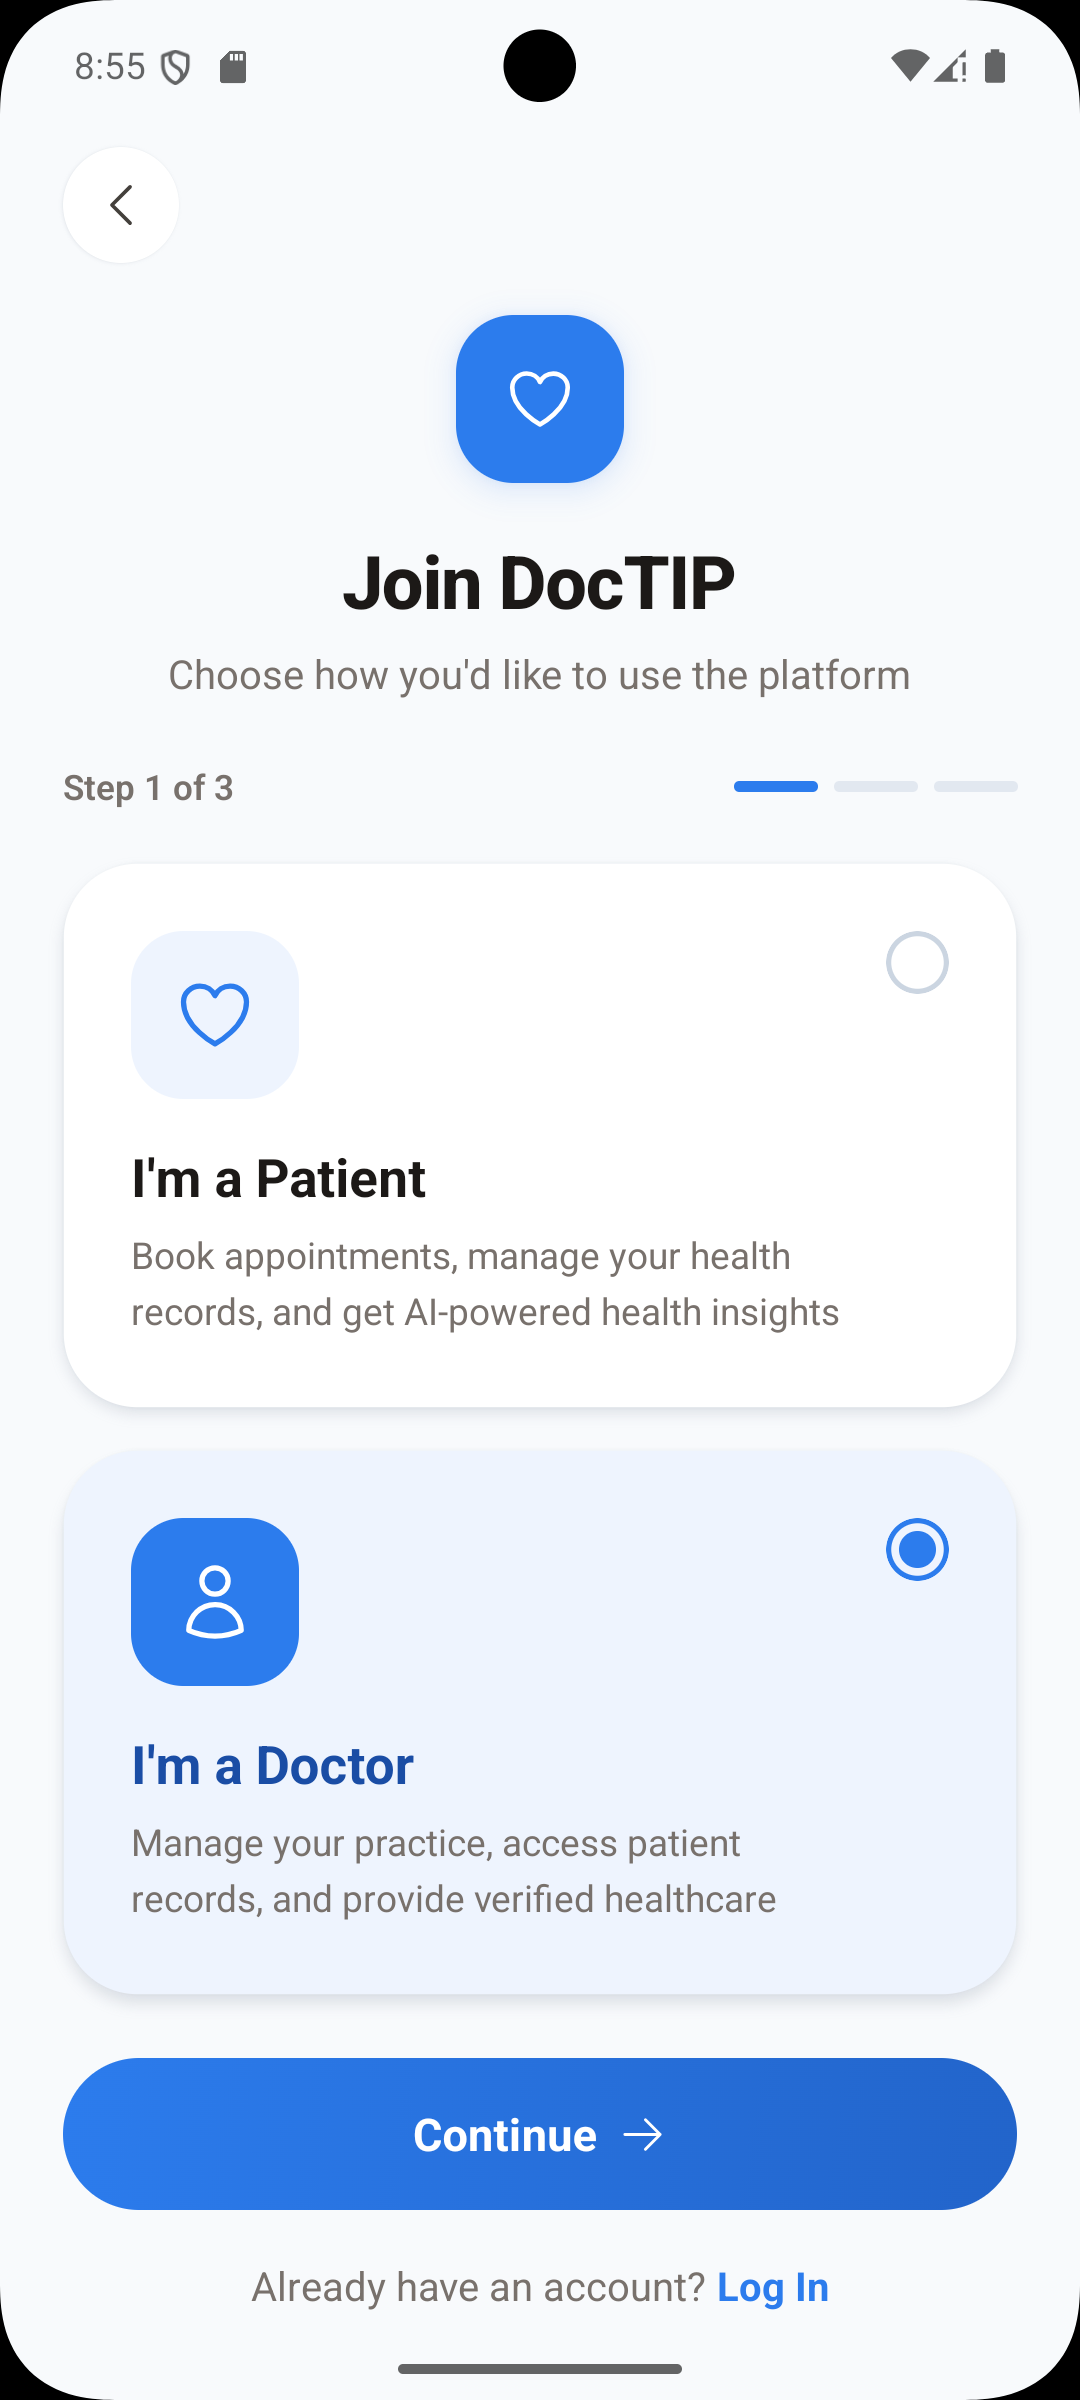
\includegraphics[width=\textwidth,height=0.58\textheight,keepaspectratio]{roledoct1.png}
    \end{minipage}\hfill
    \begin{minipage}{0.30\textwidth}
        \centering
        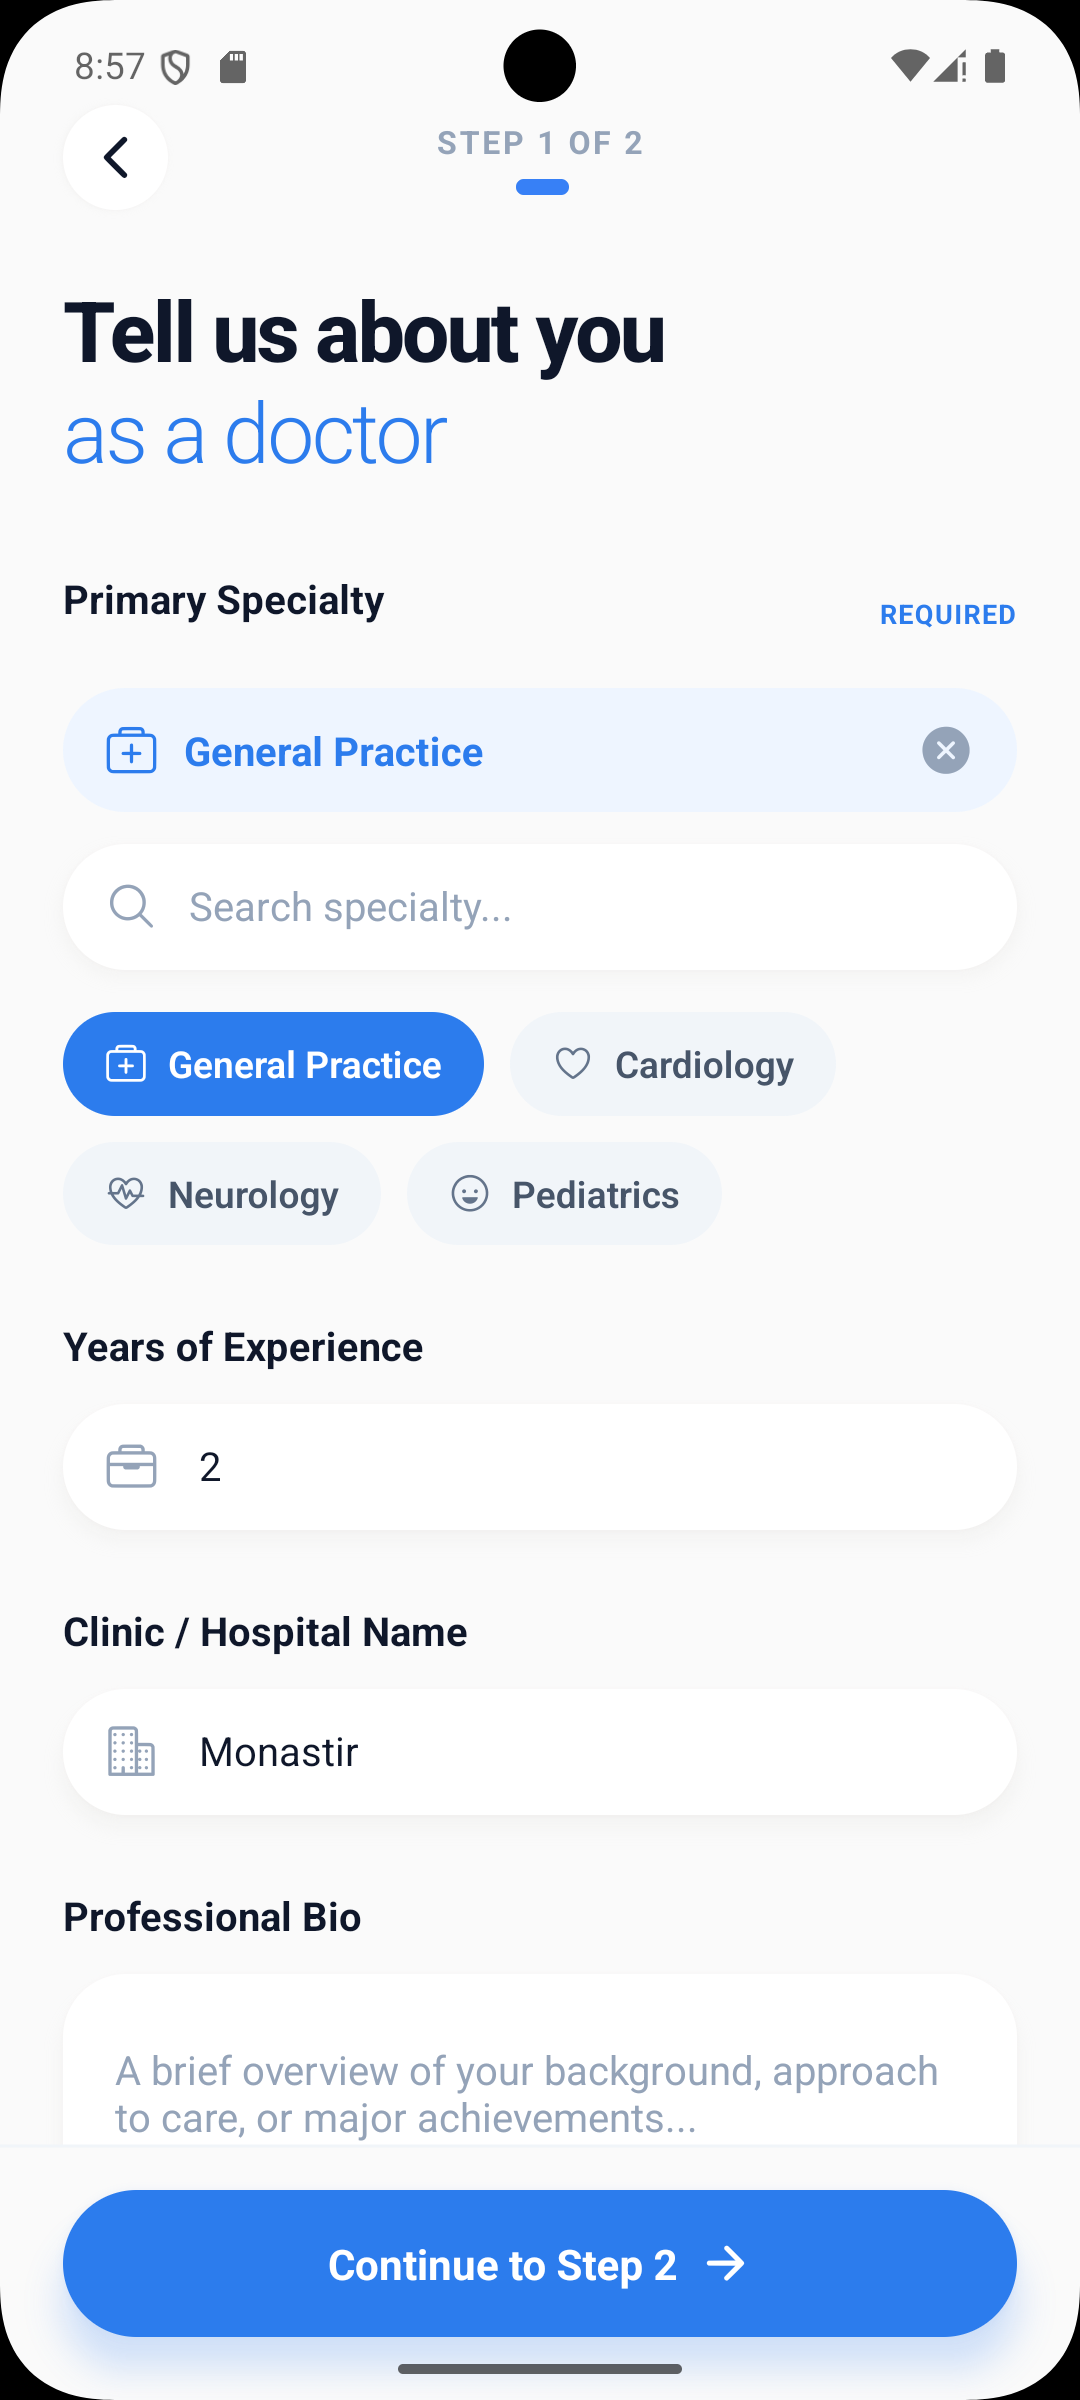
\includegraphics[width=\textwidth,height=0.58\textheight,keepaspectratio]{doc2.png}
    \end{minipage}\hfill
    \begin{minipage}{0.30\textwidth}
        \centering
        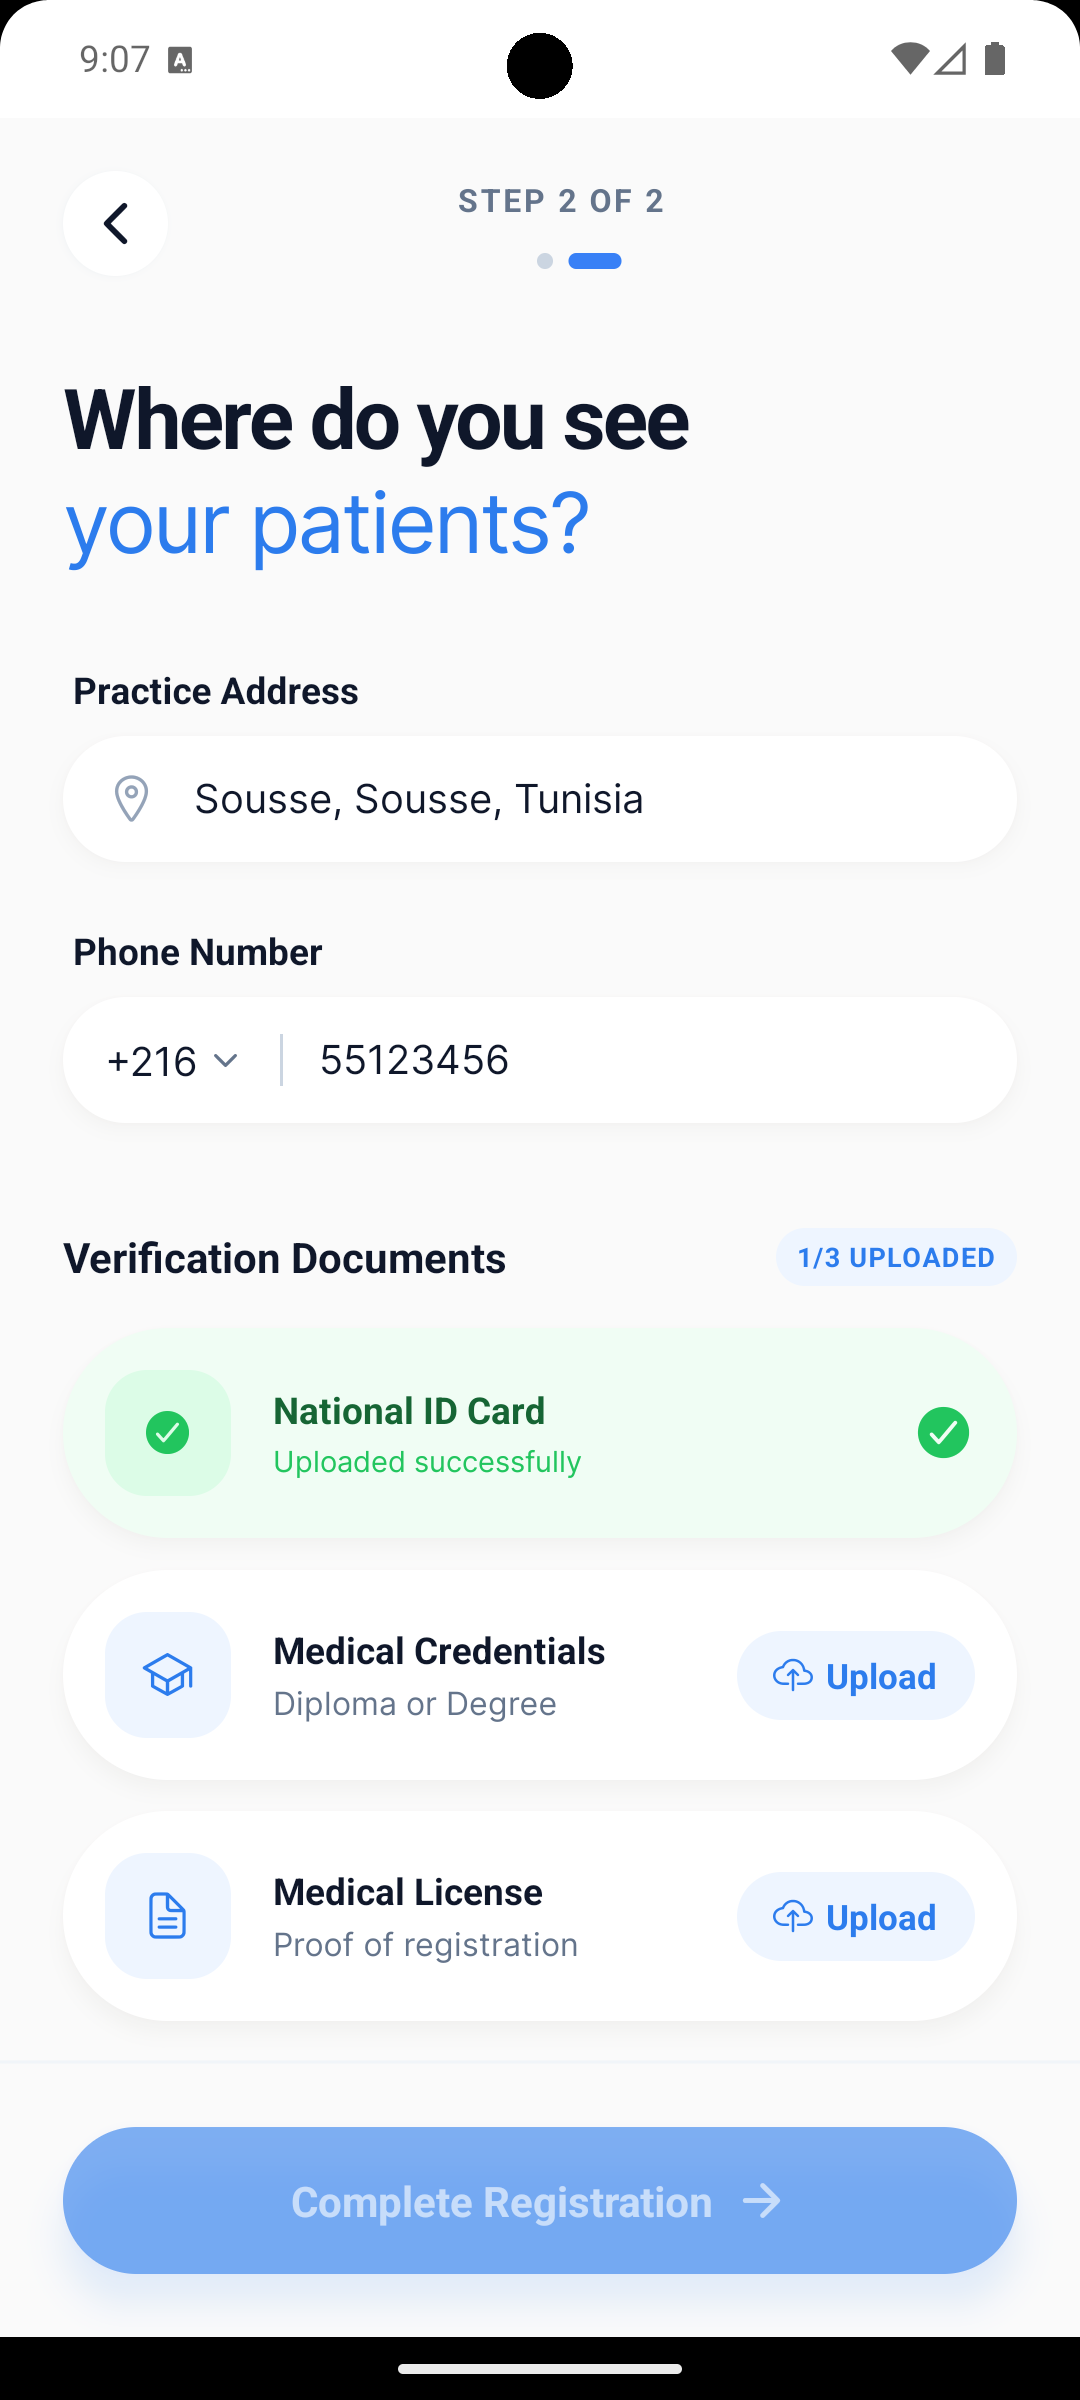
\includegraphics[width=\textwidth,height=0.58\textheight,keepaspectratio]{screen-doctor-onboarding.png}
    \end{minipage}
    \caption{Doctor Onboarding: Professional Information and Document Upload}
    \label{fig:screen doctor onboarding}
\end{figure}

\subsection{Doctor Home Dashboard}

The doctor home screen (Figure~\ref{fig:screen doctor home}) serves as the command center for daily clinical operations:

\begin{itemize}
    \item A \textbf{calendar view} with daily appointment schedule.
    \item \textbf{Real time statistics}: today's appointments, weekly consultation count, average patient rating, total linked patients.
    \item An \textbf{AI powered clinical intelligence card} providing daily clinical insights generated via OpenRouter.
    \item \textbf{Critical lab result alerts} with contextual medical icons (cardiac markers, glucose, electrolytes, hematology), enabling the doctor to identify patients requiring urgent attention.
    \item \textbf{SVG bar charts and sparklines} for trend visualization.
\end{itemize}

\begin{figure}[H]
    \centering
    \uiMobileShot{screen-doctor-home.png}
    \caption{Doctor Home Dashboard}
    \label{fig:screen doctor home}
\end{figure}

\subsection{Patient Detail Screen}

The patient detail screen provides a comprehensive view of a specific patient, organized into \textbf{three tabs}:

\begin{enumerate}
    \item \textbf{Overview:} Recovery score, recent vitals, active medications, allergies, and clinical alerts.
    \item \textbf{Records:} Complete history of diagnoses, prescriptions, lab results, and operations.
    \item \textbf{Notes:} Clinical notes written by the doctor, including AI generated SOAP notes.
\end{enumerate}

A \textbf{clinical tools grid} provides quick access to: Write Prescription, Write Lab Request, View Recovery, View Insights, Predictive Risk, Health Intelligence, Smart Follow Up, and Behavioral Health: all contextualized to the selected patient.

\begin{figure}[H]
    \centering
    \IfFileExists{figures/screen-patient-detail.png}{%
            \uiMobileShot{screen-patient-detail.png}%
    }{%
      \fcolorbox{black!20}{black!5}{%
                \parbox[c][5.4cm]{0.42\textwidth}{%
          \centering\small\itshape\color{black!50}%
          [screenshot: screen-patient-detail.png]%
        }%
      }%
    }
    \caption{Patient Detail Screen with Clinical Tools Grid}
    \label{fig:screen patient detail}
\end{figure}

\subsection{AI Clinical Notes (SOAP)}

The clinical notes screen enables AI assisted generation of \textbf{SOAP notes} (Subjective, Objective, Assessment, Plan):

\begin{itemize}
    \item Auto suggestion of medical terms: 24~chief complaints, 18~physical findings, 4~vital sign templates, 17~history elements.
    \item Real time AI generation of the complete SOAP note structure via \texttt{generateSOAPNote}.
    \item Automatic ICD 10 code suggestions.
    \item Prescription draft based on the assessment.
    \item Editable output before saving to the \texttt{clinical\_notes} table.
\end{itemize}

\begin{figure}[H]
    \centering
    \uiMobileShot{screen-clinical-notes.png}
    \caption{AI Assisted SOAP Clinical Note Generation}
    \label{fig:screen clinical notes}
\end{figure}

\subsection{AI Differential Diagnosis}

The differential diagnosis screen provides an AI powered diagnostic reasoning tool:

\begin{itemize}
    \item Input: symptoms with auto suggestion, examination findings, patient history, vital signs.
    \item Output: diagnoses ranked by confidence percentage, each with:
    \begin{itemize}
        \item ICD 10 code
        \item Red flags to watch for
        \item Missing tests (typed: lab, imaging, exam, referral)
        \item Clinical pearls and teaching points
    \end{itemize}
    \item A prominent \textbf{disclaimer} reminding that all AI suggestions are advisory only.
\end{itemize}

\subsection{ORION: AI Clinical Assistant}

The \textbf{ORION} screen provides a persistent AI chatbot interface for doctors, supporting:

\begin{itemize}
    \item Natural language clinical queries with conversation history.
    \item \textbf{Drug interaction checker}: input multiple medications and receive interaction warnings with severity and mechanism.
    \item \textbf{Clinical guidelines}: evidence based protocol summaries.
    \item \textbf{Dosage calculator}: weight based and renal adjusted dosing.
    \item Conversation persistence in the \texttt{ai\_chats} and \texttt{ai\_chat\_messages} tables.
\end{itemize}

\subsection{Risk Radar}

The Risk Radar dashboard provides a \textbf{real time overview} of all linked patients:

\begin{itemize}
    \item Patients sorted by aggregated risk score.
    \item Medication adherence rate per patient.
    \item Deterioration detection (patients whose risk scores are increasing).
    \item Quick filters by risk level.
\end{itemize}

\subsection{Voice Scribe}

The Voice Scribe feature enables \textbf{voice dictation of clinical notes}:

\begin{itemize}
    \item Four templates: progress note, procedure note, discharge summary, consultation note.
    \item Voice recording with automatic transcription.
    \item AI polish: raw transcription is refined into professional clinical text via \texttt{analyzeVoice}.
    \item Direct save to clinical notes.
\end{itemize}

\subsection{Prescription and Laboratory Management}

\textbf{Prescription creation} supports multi medication prescriptions with:

\begin{itemize}
    \item Medication search via the \textbf{RxNorm API} (standardized drug database).
    \item Dosage, frequency, administration route, duration, and time slot specification.
    \item Prescription history with status tracking (active, completed, cancelled).
\end{itemize}

\textbf{Laboratory request creation} includes:

\begin{itemize}
    \item Test selection with priority level (routine, urgent, STAT).
    \item Results viewing with per biomarker trend charts.
    \item A 5 status pipeline: requested $\rightarrow$ sample collected $\rightarrow$ processing $\rightarrow$ completed $\rightarrow$ cancelled.
\end{itemize}

\section{Presentation of the Web Administration Dashboard}

The web administration dashboard provides a comprehensive supervision interface for platform administrators. Built with React, Vite, and Tailwind CSS, it comprises \textbf{22 pages} organized around a sidebar navigation layout.

\subsection{Main Dashboard}

The main dashboard (Figure~\ref{fig:screen admin dashboard}) displays real time Key Performance Indicators (KPIs):

\begin{itemize}
    \item \textbf{Stat cards:} Total patients, active doctors (with pending count), today's appointments, total appointments, prescriptions, lab results, conversations, and average Patient Recovery Index (PRI).
    \item \textbf{Specialty distribution chart:} PieChart showing the distribution of doctors across medical specialties (top 7 specialties plus others).
    \item \textbf{Monthly trend curves:} AreaChart showing appointment volume and completed appointments over the last 6 months.
    \item \textbf{Recent activity feed:} Displays the latest platform events including new appointments and patient registrations.
    \item \textbf{Pending doctor approvals:} Section with quick approve/reject action buttons for pending doctor registrations.
\end{itemize}

\begin{figure}[H]
    \centering
    \uiWebShot{screen-admin-dashboard.png}
    \caption{Web Administration Main Dashboard}
    \label{fig:screen admin dashboard}
\end{figure}

\subsection{Doctor Management}

The doctors management page enables administrators to:

\begin{itemize}
    \item View the paginated list of all registered doctors with status filters (pending, approved, rejected, suspended).
    \item Open a detail drawer showing the doctor's profile, uploaded documents, schedule, and schedule exceptions.
    \item \textbf{Approve, reject} (with mandatory reason), or \textbf{suspend} doctor accounts.
    \item View verification document previews (national ID, medical license, professional certificates).
\end{itemize}

\begin{figure}[H]
    \centering
    \uiWebShot{screen-admin-doctors.png}
    \caption{Doctor Management and Verification Interface}
    \label{fig:screen admin doctors}
\end{figure}

\subsection{Patient Management}

The patients page provides enriched patient profiles including:

\begin{itemize}
    \item Demographic data, blood type, allergies, and chronic conditions.
    \item Current PRI score with color coded status.
    \item Activity metrics (appointment count, lab results, last visit date).
    \item Direct links to the patient's medical record history.
\end{itemize}

\subsection{Analytics}

The analytics page offers comprehensive platform level insights:

\begin{itemize}
    \item \textbf{KPI cards:} Appointment completion rate, average PRI score, total triage count, video consultation rate.
    \item \textbf{User growth chart:} Bar chart showing monthly new patients and doctors.
    \item \textbf{Appointments breakdown:} By visit type (clinic, home, video) and by status.
    \item \textbf{Top specialties:} Ranked bar chart of most booked specialties.
    \item \textbf{Triage urgency distribution:} Pie chart showing the proportion of low/moderate/high/emergency triage outcomes.
    \item Period toggle: 6 month and 12 month views.
\end{itemize}

\begin{figure}[H]
    \centering
    \uiWebShot{screen-admin-analytics.png}
    \caption{Platform Analytics Dashboard}
    \label{fig:screen admin analytics}
\end{figure}

\section{Difficulties Encountered and Solutions}

Several technical challenges were encountered during implementation:

\begin{itemize}
    \item \textbf{WebView JavaScript compatibility:} The emergency map uses Leaflet.js rendered inside a React Native WebView. ES6+ syntax (optional chaining, template literals) is not universally supported in all WebView engines. \textit{Solution:} All inline JavaScript was rewritten using ES5 compatible syntax.

    \item \textbf{Overpass API reliability:} The Overpass API (used for finding nearby medical facilities) frequently experienced timeouts or rate limiting. \textit{Solution:} A multi endpoint cascade with several mirrors and a Nominatim geocoding fallback was implemented, with per request abort timeouts to avoid blocking the UI.

    \item \textbf{AI response parsing:} Large Language Models occasionally return malformed JSON (trailing commas, markdown code fences, extra text before/after the JSON object). \textit{Solution:} The \texttt{aiJSON()} function implements robust cleaning: stripping markdown fences, removing trailing commas, extracting JSON boundaries, and falling back to brace matching extraction.

    \item \textbf{Medical data authorization:} Ensuring that doctors can only access data of their linked patients required complex Row Level Security policies spanning many database entities. \textit{Solution:} The \texttt{doctor\_patient\_relationships} table serves as the authorization backbone, referenced in every RLS policy via subqueries.

    \item \textbf{Real time message synchronization:} Maintaining message ordering and preventing duplicates across multiple devices required careful handling of Supabase Realtime subscriptions. \textit{Solution:} Messages are deduplicated by ID on the client side, and subscription reconnection logic handles network interruptions gracefully.

    \item \textbf{Push notification targeting:} Sending medication reminders to specific patients at precise times required a reliable scheduling mechanism. \textit{Solution:} A scheduled Edge Function queries pending doses in the upcoming window, groups by patient, and dispatches notifications via FCM.
\end{itemize}

\section*{Conclusion}
\phantomsection
\addcontentsline{toc}{section}{Conclusion}

This chapter presented the implementation phase of the DocTIP platform. It described the system architecture, summarized the main technology choices, and showcased the realized interfaces through the patient mobile portal, the doctor mobile portal, and the web administration dashboard. The chapter also highlighted how key requirements were translated into working features, including AI assisted triage and clinical support, secure access control, real time interactions, and administrative supervision.

% ============================================================================
%               CHAPTER 4 GENERAL CONCLUSION AND PERSPECTIVES
% ============================================================================
\clearpage

\section*{General Conclusion and Perspectives}
\phantomsection
\addcontentsline{toc}{section}{General Conclusion and Perspectives}
\label{chap:general conclusion perspectives}

This report covered the complete lifecycle of the \textbf{DocTIP} project, from needs analysis and specification to design and implementation. Developed during a final year internship at \textbf{Aderfia Incorporation}, DocTIP was conceived as an integrated medical platform that supports daily practice management while improving patient follow up through recovery monitoring and AI assisted features.

The main outcome of this work is a coherent system composed of a patient mobile portal, a doctor mobile portal, and a web administration dashboard, all connected to a secure backend. Throughout the implementation, the focus remained on delivering practical value: facilitating appointments and communication, organizing clinical information, supporting triage and clinical decision making through AI, and ensuring supervision capabilities through analytics and administration tools. Beyond the functional deliverables, this project validated key design choices related to security, scalability, and maintainability in a medical data context.

From an academic perspective, this project strengthened our skills in software architecture, cross platform development, database security, and AI integration. It also highlighted the importance of clear documentation: one of the main challenges during report writing was to keep the narrative consistent across chapters, select the right level of technical detail, and maintain alignment between figures, references, and explanations. As future perspectives, DocTIP can be extended by reinforcing offline capabilities for constrained connectivity, integrating wearable health data, enhancing AI support for voice and image based workflows, improving the pharmacy and clinical workflow integration, supporting multi clinic administration, and progressively aligning with stronger compliance and performance requirements. Overall, DocTIP demonstrates the potential of combining mobile applications, cloud services, and AI to modernize healthcare operations and patient support.

% ============================================================================
%                        REFERENCES
% ============================================================================
\clearpage
\phantomsection
\addcontentsline{toc}{chapter}{References}
{\small
\begin{thebibliography}{99}
\setlength\itemsep{3pt}
\bibitem{uml} [2026 02 05] Object Management Group, \textit{Unified Modeling Language (UML) Specification, Version 2.5.1}, OMG, 2017.
\bibitem{supabase} [2026 02 10] Supabase Inc., \textit{Supabase Documentation}, \url{https://supabase.com/docs}, 2024.
\bibitem{expo} [2026 02 14] Expo, \textit{Expo Documentation}, \url{https://docs.expo.dev}, 2024.
\bibitem{openai} [2026 02 20] OpenAI, \textit{GPT 4 Technical Report}, arXiv:2303.08774, 2023.
\bibitem{zerotrust} [2026 03 02] S. Rose, O. Borchert, S. Mitchell, and S. Connelly, \textit{Zero Trust Architecture}, NIST Special Publication 800 207, 2020.
\bibitem{agile} [2026 03 06] K. Schwaber and J. Sutherland, \textit{The Scrum Guide}, Scrum.org, 2020.
\bibitem{reactnative} [2026 03 12] Meta Platforms, \textit{React Native Documentation}, \url{https://reactnative.dev}, 2024.
\bibitem{tailwind} [2026 03 18] Tailwind Labs, \textit{Tailwind CSS Documentation}, \url{https://tailwindcss.com/docs}, 2024.
\bibitem{zustand} [2026 03 24] P. Mendez, \textit{Zustand: Bear necessities for state management in React}, \url{https://github.com/pmndrs/zustand}, 2024.
\bibitem{postgresql} [2026 04 02] The PostgreSQL Global Development Group, \textit{PostgreSQL Documentation}, \url{https://www.postgresql.org/docs/}, 2024.
\bibitem{deno} [2026 04 09] Deno Land Inc., \textit{Deno Runtime Documentation}, \url{https://deno.com/runtime}, 2024.
\bibitem{agora} [2026 04 16] Agora.io, \textit{Agora Video SDK Documentation}, \url{https://docs.agora.io}, 2024.
\bibitem{vite} [2026 04 24] E. You, \textit{Vite: Next Generation Frontend Tooling}, \url{https://vitejs.dev}, 2024.
\bibitem{leaflet} [2026 05 03] V. Agafonkin, \textit{Leaflet: An open source JavaScript library for interactive maps}, \url{https://leafletjs.com}, 2024.
\bibitem{fcm} [2026 05 11] Google, \textit{Firebase Cloud Messaging Documentation}, \url{https://firebase.google.com/docs/cloud messaging}, 2024.
\end{thebibliography}
}

\end{document}


